\startchapter{Data Reconstruction, Selection and Triggers}
\label{chapter:objects}

This chapter describes the physics objects that are reconstructed on an event-by-event basis using collision data from the ATLAS detector, and used in this DM search. It also discusses the triggers and event selection cuts that are applied to define the subsets of collision data and MC simulated data, also known as ``analysis regions", used for the search. 

\section{Object Definitions}
\label{sec:object_defs}

The goal of the ATLAS detector is to identify particles that are produced by the proton-proton collisions that take place in the centre of the detector, and to reconstruct their kinematic properties. The particle identification and reconstruction is performed using collections of measured signals in the detector sub-systems, which are broadly referred to as ``physics objects" (See Ref. \cite{physics_objects_atlas_2013} for a review of physics object reconstruction with the ATLAS detector). The physics objects used to reconstruct all particles considered in this search are described in the following sections.

\subsection{Charged Leptons}
\label{sec:charged_leptons}

The final state charged lepton produced from the leptonic decay of a \(W\) in the DH model could with approximately equal probability \cite{pdg_2020} be an electron \(e\), a muon \(\mu\) or a tau \(\tau\). Electrons are stable and as such do not decay before depositing their energy in the ATLAS detector. This allows them to be reconstructed directly using information from the inner tracker and the EM calorimeter, as discussed in Sections \ref{sec:inner_detector} and \ref{sec:EM_calo}. Muons are unstable and will ultimately decay to a \(\nu_\mu\) and a \(e\bar{\nu}_e\) pair via a virtual \(W\) boson mediator, as shown in Figure \ref{fig:muon_decay}. However, their mean lifetime of 2.2\(\mu s\), which is the average time after they are produced before they undergo the decay to \(\nu_\mu+e\bar{\nu}_e\), is long enough that muons do make it through the ATLAS detector before they decay, and are reconstructed using information from the inner tracker and the muon spectrometer, as discussed in Sections \ref{sec:inner_detector} and \ref{sec:EM_calo}. Only the \(W\rightarrow e\bar{\nu}_e\) decay is possible in the 3-body muon decay, because any other particles that a virtual \(W\) could otherwise decay to are too massive to be produced from the initial \(106~\MeV\) rest mass energy of the muon. 

\begin{figure}[hp]
	\centering
	\begin{subfigure}[t]{0.49\textwidth}
	\centering
	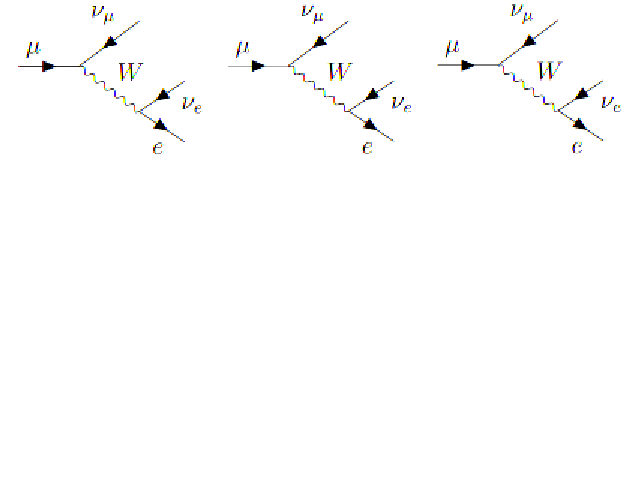
\includegraphics[width=0.5\textwidth]{Figures/5/mu_decay.pdf}
%		 \begin{tikzpicture}
%		 	\begin{feynman}
%		 		\vertex (a1); %mu
%
%		 		\vertex at ($(a1) + (1cm, 0)$) (b1); % decay to W+nu_mu
%				
%		 		\vertex at ($(b1) + (1, 0.75)$) (c1); %nu_mu
%				\vertex at ($(b1) + (1, -0.75)$) (c2); %W
%				
%				\vertex at ($(c2) + (0.75, 0.5)$) (d1); % nu_e
%				\vertex at ($(c2) + (0.75, -0.5)$) (d2); % e
%
%		 		\diagram* {
%		 		  (a1) -- [fermion, edge label=\(\mu\), near start] (b1),
%		 		  (c1) -- [fermion, edge label'=\(\nu_\mu\), near start] (b1) -- [boson, edge label=\(W\)] (c2),
%		 		  (d1) -- [fermion, edge label=\(\nu_e\), near start] (c2) -- [fermion, edge label'=\(e\), near end] (d2),
%		 		};
%		 	\end{feynman}
%		 \end{tikzpicture}
	\caption{Muon decay}
	\label{fig:muon_decay}
	\end{subfigure}
	\begin{subfigure}[t]{0.49\textwidth}
	\centering
	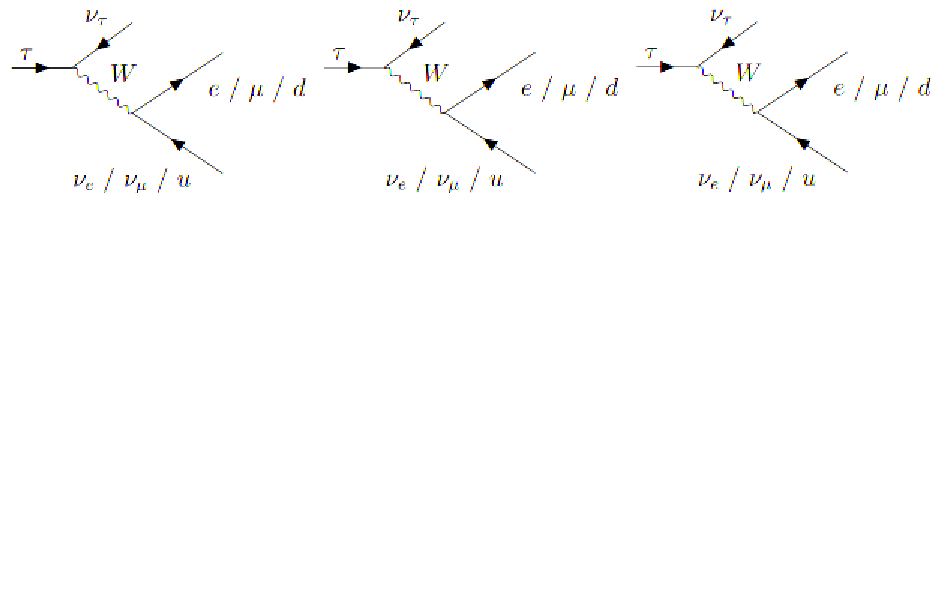
\includegraphics[width=0.75\textwidth]{Figures/5/tau_decays.pdf}
%		 \begin{tikzpicture}
%		 	\begin{feynman}
%		 		\vertex (a1); %tau
%
%		 		\vertex at ($(a1) + (1cm, 0)$) (b1); % decay to W+nu_tau
%				
%		 		\vertex at ($(b1) + (1, 0.75)$) (c1); %nu_tau
%				\vertex at ($(b1) + (1, -0.75)$) (c2); %W
%				
%				\vertex at ($(c2) + (1.5, -1)$) (d1); % nu_e / nu_mu / u / d
%				\vertex at ($(c2) + (1.5, 1)$) (d2); % e / mu / d / u
%
%		 		\diagram* {
%		 		  (a1) -- [fermion, edge label=\(\tau\), near start] (b1),
%		 		  (c1) -- [fermion, edge label'=\(\nu_\tau\), near start] (b1) -- [boson, edge label=\(W\)] (c2),
%		 		  (d1) -- [fermion, edge label={\(\nu_e\) / \(\nu_\mu\) / \(u\)}, near start] (c2) -- [fermion, edge label'={\(e\) / \(\mu\) / \(d\)}, near end] (d2),
%		 		};
%		 	\end{feynman}
%		 \end{tikzpicture}
	\caption{Tau decay}
	\label{fig:tau_decay}
	\end{subfigure}
	\caption{Decay mechanisms for muons and taus.}
	\label{fig:lepton_decays}
\end{figure}

Due to the relatively large tau mass of 1.8 \GeV, the virtual \(W\) boson in the 3-body tau decay can itself decay either leptonically to \(e\bar{\nu}_e\) or \(\mu\bar{\nu}_\mu\), or hadronically to \(d\bar{u}\), as shown in Figure \ref{fig:tau_decay}. As a result of the additional decay channels, tau decays proceed with a much shorter mean lifetime of 0.3ps compared with that of the muon. Because of this relatively short lifetime, taus will decay before passing through the ATLAS detector, and as such it is their leptonic or hadronic decay products that are actually measured in the detector \cite{ATLAS-CONF-2017-029}. As will be discussed in Section \ref{sec:evt_selections} below, the selections applied for this analysis require that events have exactly one electron or muon in the final state in order to be considered for the search. As a result, the search is sensitive to \(s\rightarrow WW\) decays in which the leptonically decaying \(W\) decays to \(\tau\nu_\tau\) only in the case where the \(\tau\) decays leptonically to produce a single energetic electron or muon in the final state. This leptonic \(tau\) decay mode occurs with a 35\% branching fraction \cite{ATLAS-CONF-2017-029}.

\subsubsection{Electrons}

As discussed in Section \ref{sec:EM_calo}, electron objects are reconstructed from clusters of energy deposits in the electromagnetic calorimeter that are associated with tracks in the inner detector, and calibrated to the EM scale. Detailed information about electron reconstruction, identification, and calibration can be found in Refs.~\cite{ATL-PHYS-PUB-2017-022}, \cite{PERF-2017-01} and \cite{PERF-2017-03}. To accommodate the differing needs of the various studies that make use of electron objects, ATLAS reconstructs these objects at several levels of identification and isolation efficiency, where the various efficiency levels are referred to as ``working points", the names of which are typically variants of \emph{Loose}, \emph{Medium} and \emph{Tight} for reasons that will be discussed in the following paragraphs.

The identification efficiency refers to the probability that an electron passing through the detector will be correctly reconstructed and identified as such. In general, a higher efficiency is achieved by loosening electron identification criteria, which comes at the cost of an increased background acceptance. The increased background acceptance means that reconstructed objects have a higher probability of being incorrectly identified as having originated from an electron. 

Electron isolation tackles a slightly different, though related, challenge in comparison with identification. The goal of isolation is to separate the so-called ``prompt" electrons that are produced from the primary decay processes of heavy mediators produced in the \(pp\) collisions from background processes such as semileptonic quark decays, hadrons misidentified as leptons and photons that convert into \(e^+e^-\) pairs before reaching the EM calorimeter. It is generally found that reconstructed objects that originate from prompt electrons can be characterized by a relative absence of (i.e. isolation from) significant activity in a small angular radius \(R\) around the object in the space of \(\eta\times\phi\). In analogy with the identification efficiency, a high isolation efficiency is achieved by loosening the criteria for defining an object as isolated. As such, loosening isolation criteria will improve the probability that the prompt electrons targeted by the isolation requirement are identified as isolated objects, at the cost of an increase in the rate at which objects that originate from background processes are also identified as isolated.
 
Two types of electrons are defined for the search based on different sets of criteria.

\emph{Baseline} electrons use the \emph{Loose} working point for both identification and isolation. Isolation is measured within a fixed angular radius of \(\Delta R=0.2\) around the reconstructed electron object \cite{PERF-2017-01}. The \emph{Loose} identification working point is measured in dedicated studies performed within the ATLAS collaboration to have an efficiency of 93\% \cite{PERF-2017-01} for identifying prompt electrons with \(E_T=40~\GeV\). The \emph{Loose} isolation working point has a total measured efficiency of 98\% \cite{PERF-2017-01}. Because of their relatively high efficiency, \emph{baseline} electrons are used to veto the presence of additional electrons in the final state.

\emph{Signal} electrons are designed reconstruct prompt electrons with high purity. They are required to satisfy the \emph{Medium} identification criteria, which are measured to have an 88\% efficiency \cite{PERF-2017-01}, and \emph{Loose} isolation criteria.

Both types of electrons are required to have \(\pT > 7~\GeV\) and a pseudorapidity in the range of \(|\eta| < 2.47\).

\subsubsection{Muons}

As described in Section \ref{sec:muon_spec}, muons are reconstructed using information from the the inner detector and the muon spectrometer. Detailed information about muon reconstruction, identification and calibration can be found in Refs. \cite{PERF-2015-10} and \cite{ATL-PHYS-PROC-2018-052}. As is the case with electron objects, muon objects are reconstructed at several identification and isolation working points, and two definitions for muons are considered for this analysis:

\emph{Baseline} muons do not have any isolation requirement, but are required to satisfy the \emph{Loose} identification criteria, with a measured efficiency of 98\% for \(20~\GeV<p_{T, \mu}<100~\GeV\) \cite{PERF-2015-10}.

\emph{Signal} muons are designed to have a relatively high purity, and must satisfy the \emph{Medium} identification criteria, with a 96\% efficiency for \(20~\GeV<p_{T, \mu}<100~\GeV\) \cite{PERF-2015-10}. Signal muons are additionally required to pass a set of tight isolation criteria referred to as \emph{TightTrackOnly\_VarRad} \cite{ATL-PHYS-PROC-2018-052}. These tight isolation criteria use information from the inner tracker, and are defined within an angular radius \(\Delta R\) around the reconstructed muon object that depends on the \pt of the muon object.

Both types of muons use a threshold of \(\pt > 7~\GeV \). 

Baseline muons are required to have pseudorapidity in the range of  \(|\eta| < 2.7\). For signal muons, a tighter pseudorapidity range of \(|\eta| < 2.5\) is required to ensure that the muons are well measured in the inner detector as well as the muon spectrometer. 

\subsection{Small-radius \aktfour jets}
\label{sec:atk4_jets}

As discussed in detail in Section \ref{sec:had_calo}, quarks and gluons induce showers of energy deposits in the calorimeter known as jets. This search uses the ``particle flow algorithm" \cite{PERF-2015-09} to reconstruct objects associated with the energy deposits in the hadronic calorimeter. The particle flow algorithm matches signals from the inner tracker with topologically connected clusters of energy deposits in the calorimeter known as ``topo-clusters" with the aim of forming objects that represent individual charged particles. The energy deposited in the calorimeter by these identified charged particle objects is removed, leaving behind an ensemble of ``particle flow objects" that consist of the remaining calorimeter energy and tracks. The anti-\(k_t\) algorithm described in Ref. \cite{akt_algo} is then used to reconstruct jets using these particle flow objects. A range of jet radii \(R\)\footnote{See Eq. \ref{eq:jet_radius} for the definition of the angular radius \(R\).} may be chosen within which the \akt algorithm should include particle flow objects for jet reconstruction. The choice of \(R\) depends on the kinematics, and on anticipated origins of the quark or gluon that initiated the shower (see discussion in Section \ref{sec:had_calo} for more details).

As discussed in Chapter \ref{chapter:dh_model}, the final state signature of the DH model targeted in this search involves a pair of energetic \(W\) bosons in the final state, one of which decays leptonically to a \(\ell\nu\) pair, and the other hadronically to a pair of quarks. If the boost of the hadronically decaying \(W\) is sufficiently low, the angular separation between the two quarks may be large enough that the quarks are most effectively reconstructed as two separate jets, each with a small jet radius \(R\). In the so-called ``resolved" regime of the search, the two sets of energy deposits in the calorimeter produced by the \(W\rightarrow qq\) decay are so separated that it is not even possible to reconstruct the two quarks within a single large-radius jet. For this search, these so-called ``\smallR" jets are reconstructed with a jet radius of \(R=0.4\).

After all \smallR jets in the final state are reconstructed and fully calibrated, as described in Ref. \cite{ATLAS-CONF-2015-037}, only jets with \(\pt > 20~\GeV\) and \(|\eta| < 2.5\) are considered for the search. Jet cleaning \cite{ATLAS-CONF-2015-029} with the \emph{TightBad} working point is applied to suppress noise in the calorimeter, as well as background jets that are not produced from the primary \(pp\) collision. The jet vertex tagger \cite{ATLAS-CONF-2014-018} is applied with the \emph{Tight} working point to suppress pileup jets (see Ref. \cite{pileup} for a discussion of pileup and its simulation in the ATLAS detector) from other \(pp\) interactions in the same and neighbouring bunch crossings - see Section \ref{sec:evt_wts} for a more detailed discussion of pileup events. 
%As described in Section \ref{sec:resolved_w_cand} below, these jets are used in the analysis to identify quarks originating from the hadronically-decaying \(W\) boson in the DH signal model in the resolved regime, and to reconstruct the \(W\) boson in this regime.

\subsubsection{\btag}
\label{sec:btag}

When \(b\) quarks are produced by \(pp\) collisions in the ATLAS detector, they immediately form ``\(b\)-hadrons" due to colour confinement. The \(b\)-hadrons subsequently decay primarily via the weak force to form lighter hadrons. The so-called secondary decays of b-hadrons occur with a typical lifetime of \(\sim 1.5\)ps \cite{pdg_2020}, and as a result the b-hadrons can travel several millimeters from the primary \(pp\) interaction point \cite{ATLAS-CONF-2018-006} before undergoing secondary decay. The displaced secondary vertex represents a signature of \(b\)-hadron decay in the ATLAS detector. It can be reconstructed using precision tracking of charged particles provided by the inner detector, and used to assign a ``\(b\) tag" to hadronic jets in the ATLAS calorimeter to identify them as having originated from the decay of a \(b\)-hadron. This so-called ``\bjet tagging" is performed with the \verb|DL1r| algorithm \cite{ATLAS-CONF-2018-006}, which uses a deep learning method for the identification. A fixed working point with a 77\% efficiency is used. \btagged jets are vetoed in the signal region to reduce the background of SM \ttbar and single-top processes (see Section \ref{sec:dominant_bkgs} for details).

\subsection{Resolved \(W\) Candidate}
\label{sec:resolved_w_cand}

As described in Section \ref{sec:atk4_jets} above, the pair of quarks produced by the hadronic decay of the \(W\) boson in the signal model are reconstructed as two resolved \smallR jets in the less-boosted resolved regime. The parent \(W\) boson can then be reconstructed from \smallR jets induced by its daughter quarks using the combined energy and momentum of the \smallR jet pair. Given that \smallR jets can also be produced by, for example, initial-state radiation and pileup, it is quite common for there to be more than two \smallR jets reconstructed in the final state. These additional jet sources complicate the task of identifying which of the reconstructed \smallR jets in a given event should be associated with the \(W\rightarrow qq\) in the signal model. For events with more than two \smallR jets in the final state, the pair of \smallR jets whose combined invariant mass is closest to the \(W\) boson mass is assumed to have originated from the \(W\) decay, and used to reconstruct the \(W\) boson candidate. The algorithm for this jet identification and \(W\) boson reconstruction is as follows:

\begin{itemize}
\item Construct all possible combinations of two \smallR jets (a.k.a. ``dijet pairs") in the final state.
\item For each such candidate dijet pair, \(j_1\) and \(j_2\), sum the four-momenta of the reconstructed jets, \(\mathbf{p}_{j_1,j_2} = \mathbf{p}_{j_1} + \mathbf{p}_{j_2}\), and calculate their combined invariant mass: 

\begin{equation}
\label{eq:dijet_invt_mass}
M_{j_1,j_2} = \sqrt{\mathbf{p}_{j_1,j_2} \cdot \mathbf{p}_{j_1,j_2} } 
\end{equation}
\item Select the dijet pair whose invariant mass is closest to the \(W\) boson mass of \(80.4~\GeV\) \cite{pdg_2020} as the \smallR jets to be associated with the \(W\rightarrow q\bar{q}\) decay.
\item Reconstruct the hadronically decaying \(W\) boson candidate using the dijet pair with four-momentum \(\mathbf{p}_{j_1,j_2}\).
\end{itemize}

Figure \ref{fig:resolved_Wmass_reco} shows distributions of the reconstructed \(W\) boson candidate mass for MC simulated events generated for a range of \ms and \mZp after application of the baseline event selections presented in Section \ref{sec:evt_selections}, with the additional requirement that there be at least two \smallR jets in the final state. The distributions are in general well centred around the \(W\) boson mass.

\begin{figure}[h]
	\centering
	\begin{subfigure}[b]{0.49\textwidth}
	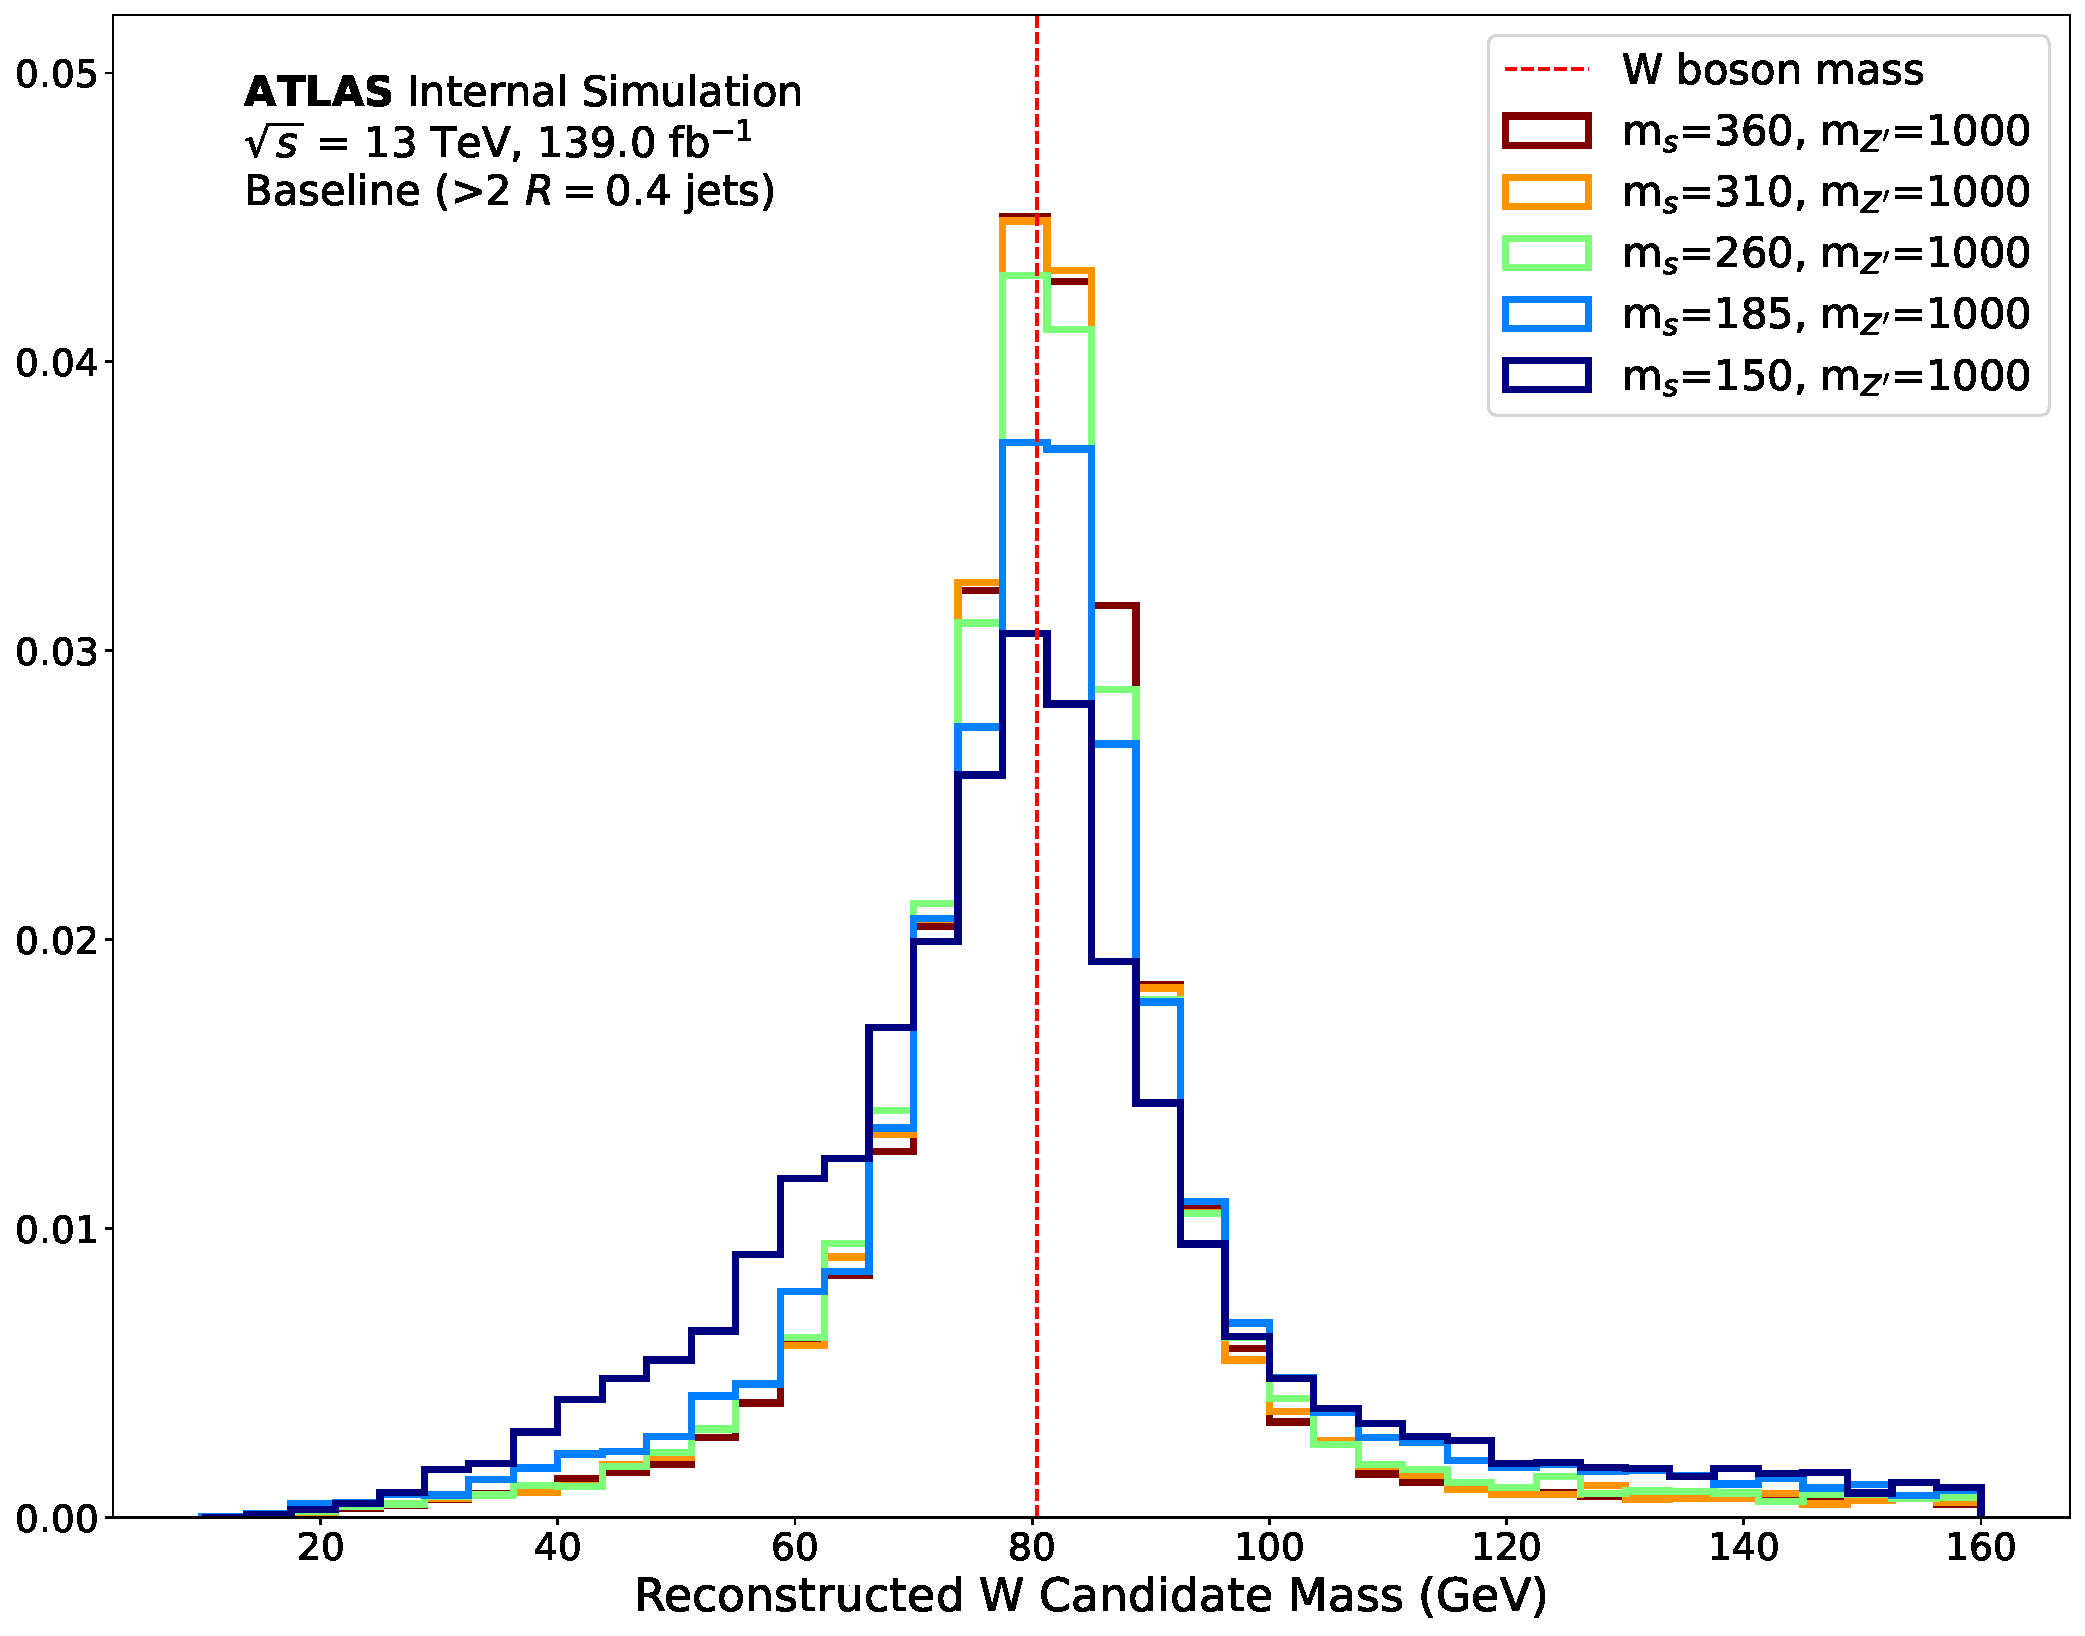
\includegraphics[width=0.95\textwidth]{Figures/5/WCand_m_ms.pdf}
	\caption{\mZp fixed, \ms varied}
	\label{fig:resolved_Wmass_reco_ms}
	\end{subfigure}
	\begin{subfigure}[b]{0.49\textwidth}
	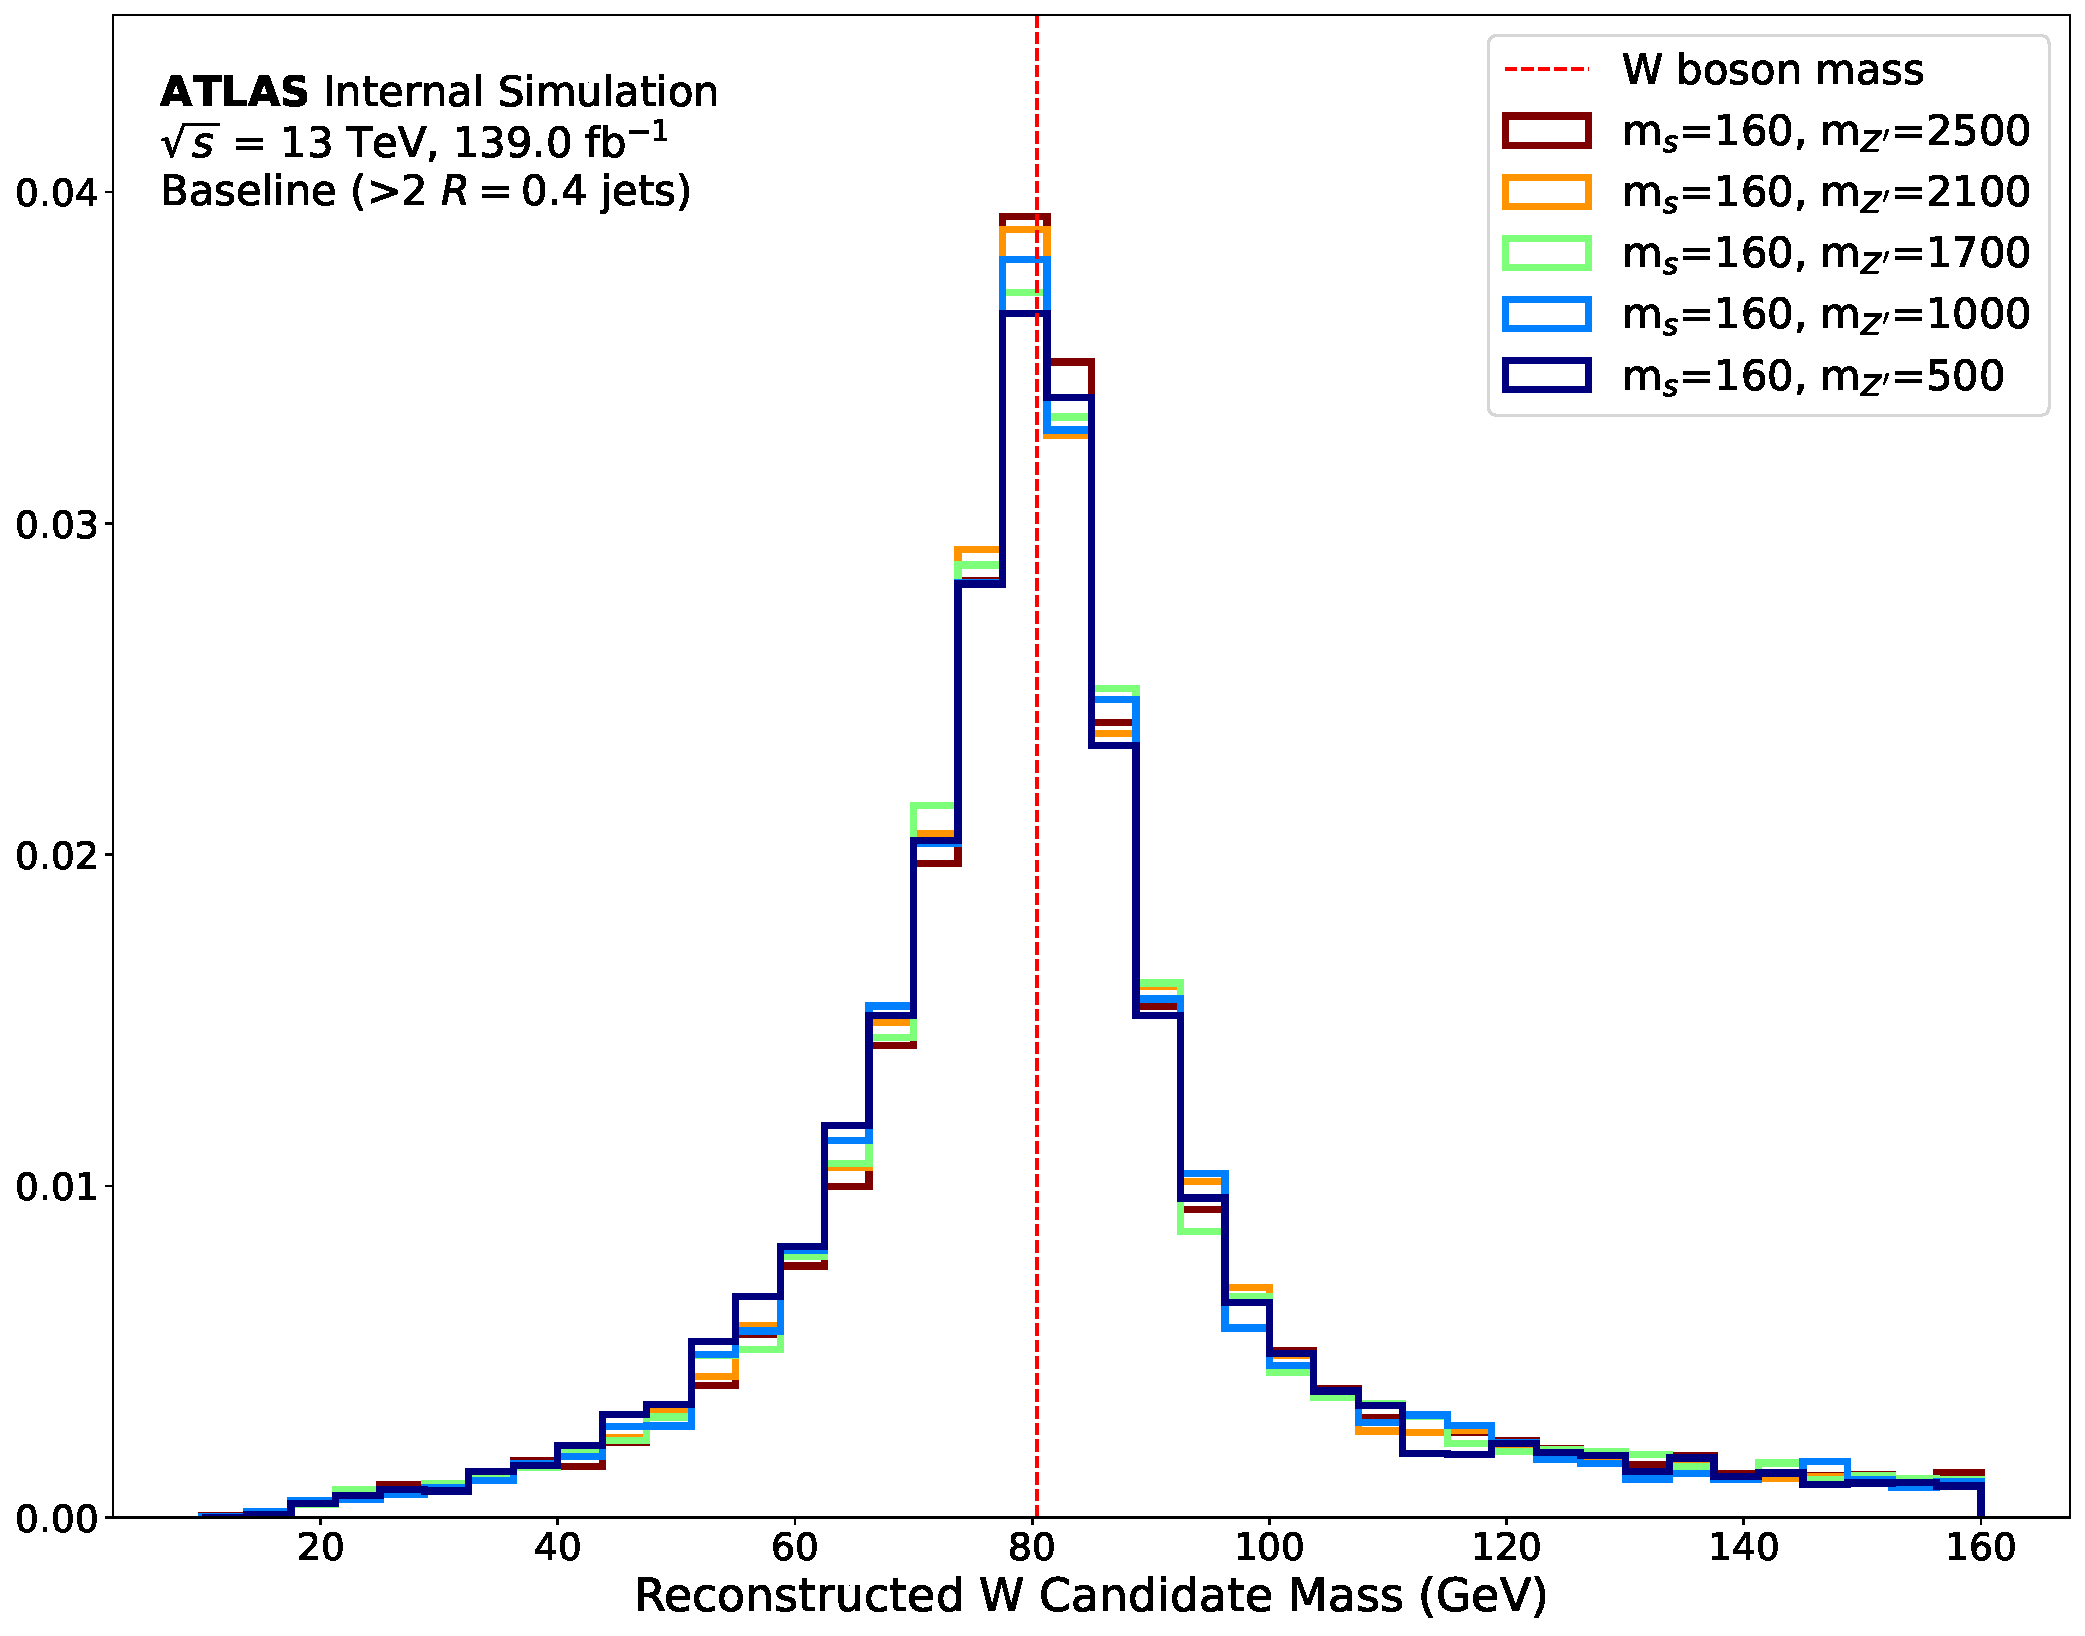
\includegraphics[width=0.95\textwidth]{Figures/5/WCand_m_mZp.pdf}
	\caption{\ms fixed, \mZp varied}
	\label{fig:resolved_Wmass_reco_mZp}
	\end{subfigure}
	\caption[Distributions of the reconstructed W candidate mass for MC simulated events produced with the DH signal model over a range of \ms and \mZp.]{Distributions of the reconstructed W candidate mass for MC simulated events produced with the DH signal model over a range of \ms and \mZp. All events included in the distributions are required to have passed the baseline event selection described in Section \ref{sec:evt_selections}, and to have at least two \smallR jets in the final state. The red dashed vertical line is placed at the \(W\) boson mass of 80.4 \GeV. Distributions are normalized to unit area.}
	\label{fig:resolved_Wmass_reco}
\end{figure}

\subsection{Track-Assisted Reclustered Jets (Merged \(W\) Candidate)}
\label{sec:TAR_jets}

If the hadronically decaying \(W\) boson is produced with a sufficiently large momentum (i.e. boost), the jets produced by the \(q\bar{q}\) pair may be sufficiently collimated (i.e. ``merged") that they are most effectively reconstructed as a single multi-pronged \largeR jet, as opposed to the resolved \smallR jets used for \(W\) reconstruction in the resolved regime (see Sections \ref{sec:atk4_jets} and \ref{sec:resolved_w_cand} above for details). 

Since the signal model predicts that charged particle tracks and energy deposits in the detector will have originated primarily from the two quarks produced by the \(W\rightarrow q\bar{q}\) decay in the signal model, it is important to reconstruct the large-radius jet in this so-called merged regime with as much detailed kinematic and substructure information as possible. This information is used in the search to help identify whether the hadronic activity contained within a \largeR jet is consistent with having been induced by two energetic quarks originating from a \(W\) parent, as predicted by the signal model. Such features include the combined invariant mass \mTAR of all particles associated with the jet, which would be expected to be consistent with the \(W\) boson mass within detector resolution. Important substructure information includes variables that aim to quantify the number of distinct ``prongs" of localized energy deposition within the jet, which can be correlated to the number of high-\pt strongly interacting particles whose energy deposits are included in the jet (two such prongs would be expected for the signal model). 

This search uses the track-assisted reclustered (TAR) jet algorithm \cite{TAR_algo} for \largeR jet reconstruction in the merged regime. In this regime, the highest-\pt TAR jet reconstructed with a radius parameter of \(R=1.0\) is used to reconstruct the hadronically decaying \(W\) boson (\(W_\text{had}\)) in the DH signal model. Whereas most \largeR jet reconstruction techniques rely on energy deposits in the calorimeter to reconstruct the jet substructure information, TAR jets are designed to profit from the superior resolution of the inner tracker for improved substructure reconstruction by matching charged particle tracks with energy deposits in the calorimeter. 

\subsubsection{TAR Algorithm}
\label{sec:TAR_algo}

For this search, \(R=0.2\) \smallR jets are used to reconstruct energy deposits in the calorimeter, and are input to the TAR algorithm along with tracks measured by the inner detector that satisfy a set of quality criteria summarized in Table \ref{tab:TARparameters}. The TAR algorithm \cite{TAR_algo} is as follows: the input \(R=0.2\) \smallR ``subjets" are reclustered using the \akt algorithm with \(R=1.0\) to form \largeR jets. A trimming procedure is applied to mitigate the effects of pileup and background QCD processes within the triggered event that do not originate from the hard interaction. The trimming procedure removes any of the input subjets that carry less than a fraction \(\fcut=0.05\) of the total transverse momentum of the \largeR jet: \(\pt^\text{subjet}/\pt^\text{\largeR jet} < 0.05\).  The tracks from the inner detector are then matched to the remaining \smallR subjets using the ghost association procedure described in Ref. \cite{ghost_association_2008}, if possible. Any tracks that cannot be matched to subjets using ghost association are instead matched to the nearest subjet, provided that there is a jet within an angular radius \(\Delta R=0.3\) of the track. To account for the energy of the neutral hadronic jet components, which do not leave tracks in the inner detector, the \pt of each track is scaled such that the summed \pt of all tracks matched to a given subjet will evaluate to the energy of the subjet as measured by the calorimeter:

\begin{equation}
\label{eq:tar_track_pt_scaling}
\pt^\text{track, new} = \pt^\text{track, old} \times \frac{p_{T,j}^\text{subjet}}{\sum_{i \in j}p_{T, i}^\text{track, old}}
\end{equation}

\noindent where the index \(i\) runs over all tracks matched to the subjet \(j\). The rescaled tracks and remaining subjets are again reclustered using the \akt algorithm to form the final \largeR TAR jet.

While the kinematic properties of the TAR jets are calculated from the constituent \smallR jets, the jet substructure and mass \(m^\text{TAR}\) are calculated from the constituent tracks. Figure \ref{fig:TARAlg} shows a visual summary of the basic TAR algorithm. 

\subsubsection{TAR-lepton Disentanglement}

The analysis applies the TAR algorithm to \(R=0.2\) \smallR jets and tracks that have undergone a ``TAR-lepton disentanglement" preselection to remove tracks associated with any reconstructed baseline electrons or muons, as well as any \(R=0.2\) jets that overlapped with the baseline electron tracks. This preselection is helpful given the final state targeted in the search, because the charged lepton produced by the leptonic \(W\rightarrow \ell\nu\) decay often falls within the \(R=1.0\) cone of the TAR jet, as illustrated in Figure \ref{fig:TAR_lepton_overlap_illustration}. This TAR-lepton overlap disrupts the jet reconstruction, particularly due to the additional jet energy induced by calorimetric clusters created in the \largeR jet by the overlapping electron.

\begin{figure}[H]
  \centering
     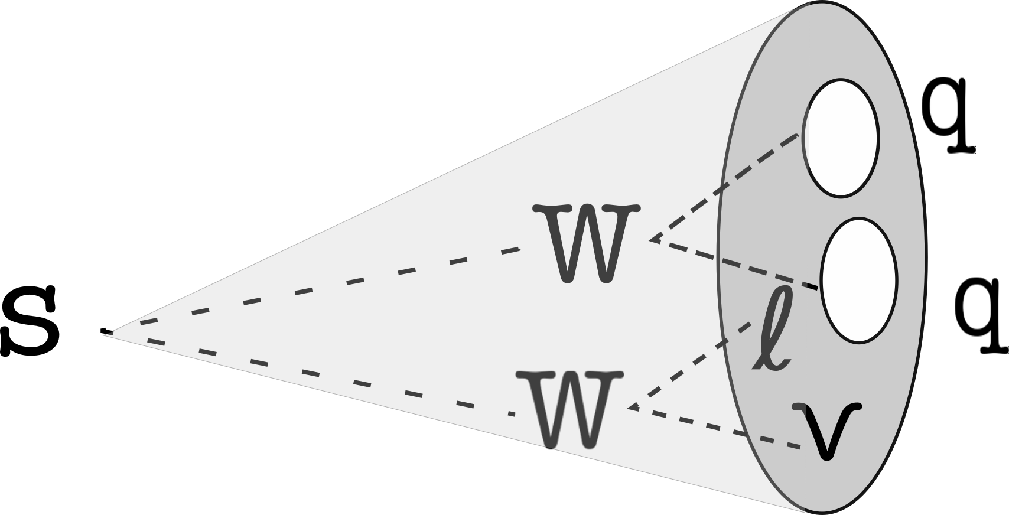
\includegraphics[width = 0.3\textwidth]{Figures/5/lepton_overlap.pdf}
     \caption[Illustration of a final state with TAR-lepton overlap.]{Illustration of the final state scenario in which the charged lepton produced by the leptonic \(W\rightarrow \ell\nu\) decay overlaps with the \largeR TAR jet reconstructed from the hadronic \(W\rightarrow qq\) decay.}
     \label{fig:TAR_lepton_overlap_illustration}
  \end{figure}
  
Figure \ref{fig:TARdisentaglementplots} shows a comparison of the distributions of reconstructed TAR jet mass \mTAR either without or with the TAR-lepton disentanglement preselection applied, for MC simulated events produced with the DH signal model at several representative \ms and \mZp, in which the reconstructed electron in the final state overlaps with the highest-\pt reconstructed TAR jet. For all the signal points, the TAR-lepton disentanglement preselection is found to substantially improve the ability of the TAR algorithm to reconstruct TAR jets with \mTAR near the \(W\) boson mass, as would be expected for the signal model.
  
\begin{figure}[H]
\centering
\begin{subfigure}{0.49\textwidth}
   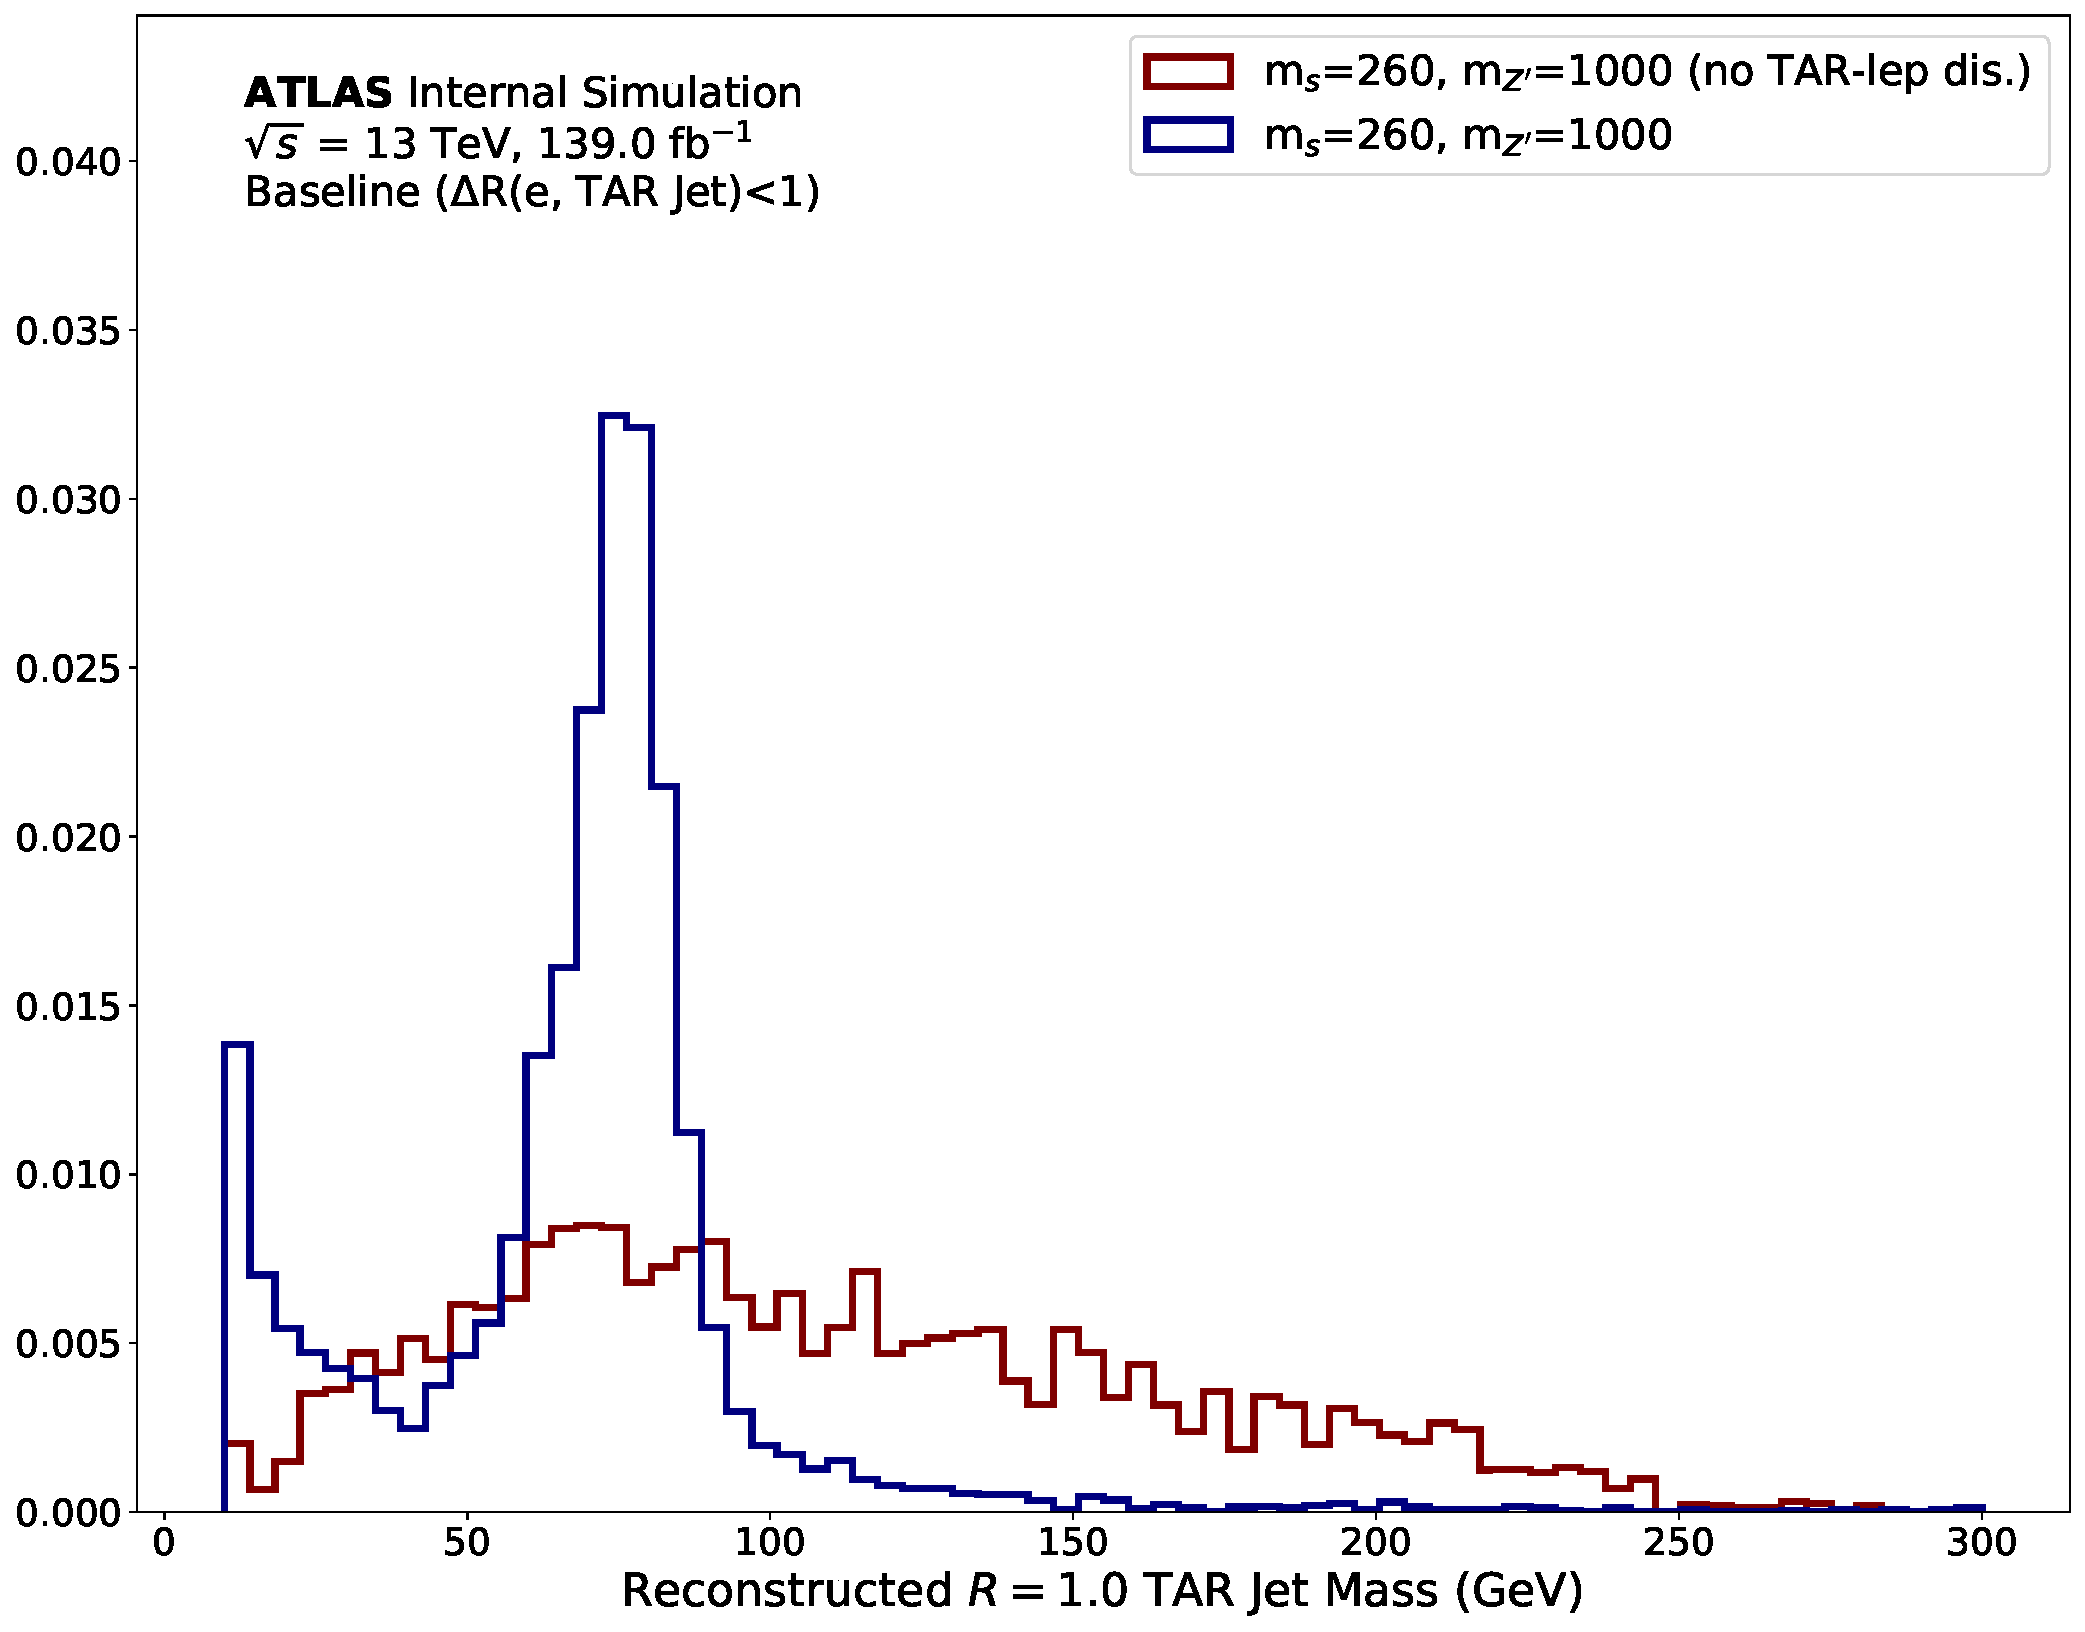
\includegraphics[width = 0.95\textwidth]{Figures/5/zp1000_dm200_dh260_disentanglement.pdf}
   \caption{\((\ms, \mZp) = (260, 1000)~\GeV\)}
   \label{fig:TARdisentaglementplots_zp1000_dh260}
\end{subfigure}
\begin{subfigure}{0.49\textwidth}
   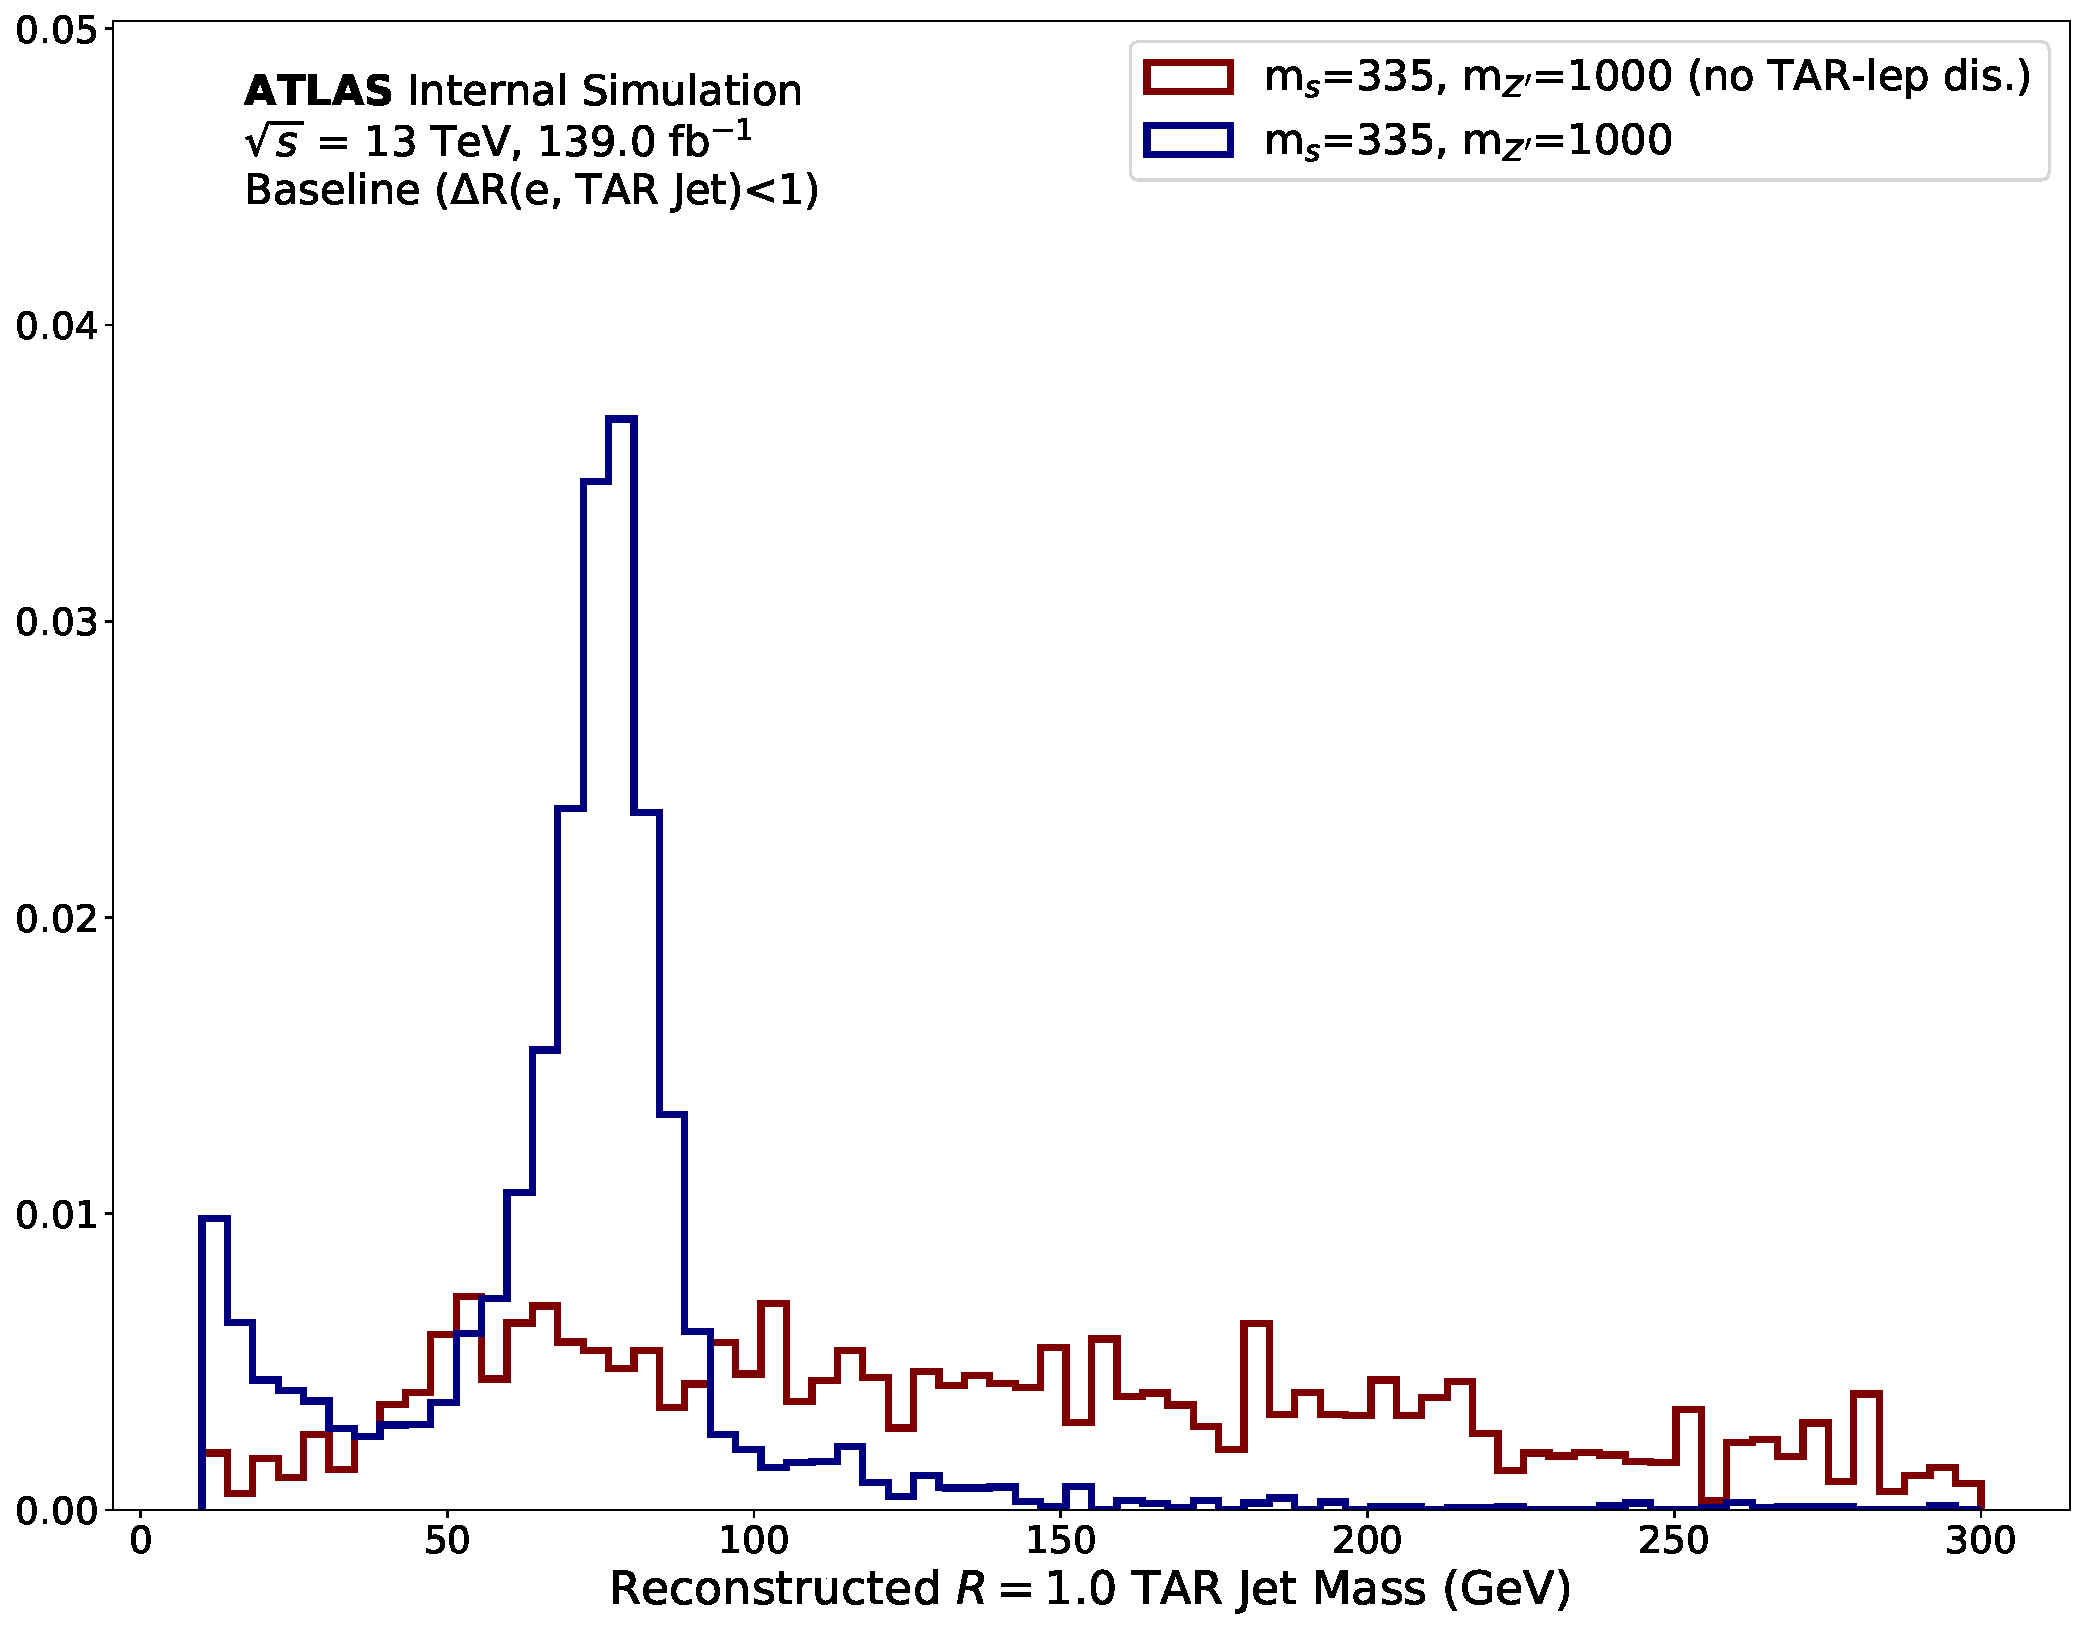
\includegraphics[width = 0.95\textwidth]{Figures/5/zp1000_dm200_dh335_disentanglement.pdf}
   \caption{\((\ms, \mZp) = (335, 1000)~\GeV\)}
   \label{fig:TARdisentaglementplots_zp1000_dh335}
\end{subfigure}
   \caption[Distributions of \mTAR at several representative \ms and \mZp, with and without application of the lepton disentanglement preselection.]{Distributions of \mTAR for the leading-\pt TAR jet in MC simulated events generated for the DH signal model process with semileptonic \(WW\) decay at several representative \ms and \mZp, with and without application of the lepton disentanglement preselection. Events included in the distributions are required to have one signal electron and at least one reconstructed TAR jet, both within an angular radius of \(\Delta R=1.0\). Distributions are normalized to unit area.}
   \label{fig:TARdisentaglementplots}
\end{figure}

\subsubsection{Summary of the TAR Procedure}

The following steps summarize the algorithm used to construct the TAR jets used in this search (steps with a * are included to disentangle leptons):
\begin{itemize}
  \item Tracks and calibrated \akt \(R=0.2\) jets are chosen as input to the algorithm.
  \item Tracks associated with a baseline muon or electron are removed from the input collection (*).
  \item \(R=0.2\) jets overlapping with a baseline electron (\(\DeltaR<0.2\)) are removed from the input collection (*).
  \item The remaining \(R=0.2\) subjets are reclustered using the \akt algorithm into \(R=1.0\) jets, and trimmed using the \(p_T\) fraction \(\fcut=0.05\).
  \item Input tracks are matched to \(R=0.2\) subjets that remain after trimming, if possible, using ghost association.
  \item Tracks that remain unassociated are matched to the nearest \akt \(R=0.2\) jet within \(\DeltaR<0.3\).
  \item The \pt of each track is rescaled using the \pt of the jet to which it is matched using Eq. \ref{eq:tar_track_pt_scaling}. This rescaling accounts for the missing neutral momentum, which is measured at calorimeter level but is not present at tracker level.
  \item Finally, jet substructure variables and  \(m^\text{TAR}\) are calculated using the rescaled matched tracks.
\end{itemize}
The parameters of the TAR algorithm used are summarized in Table \ref{tab:TARparameters}. \\

\begin{figure}[htb]
  \centering
     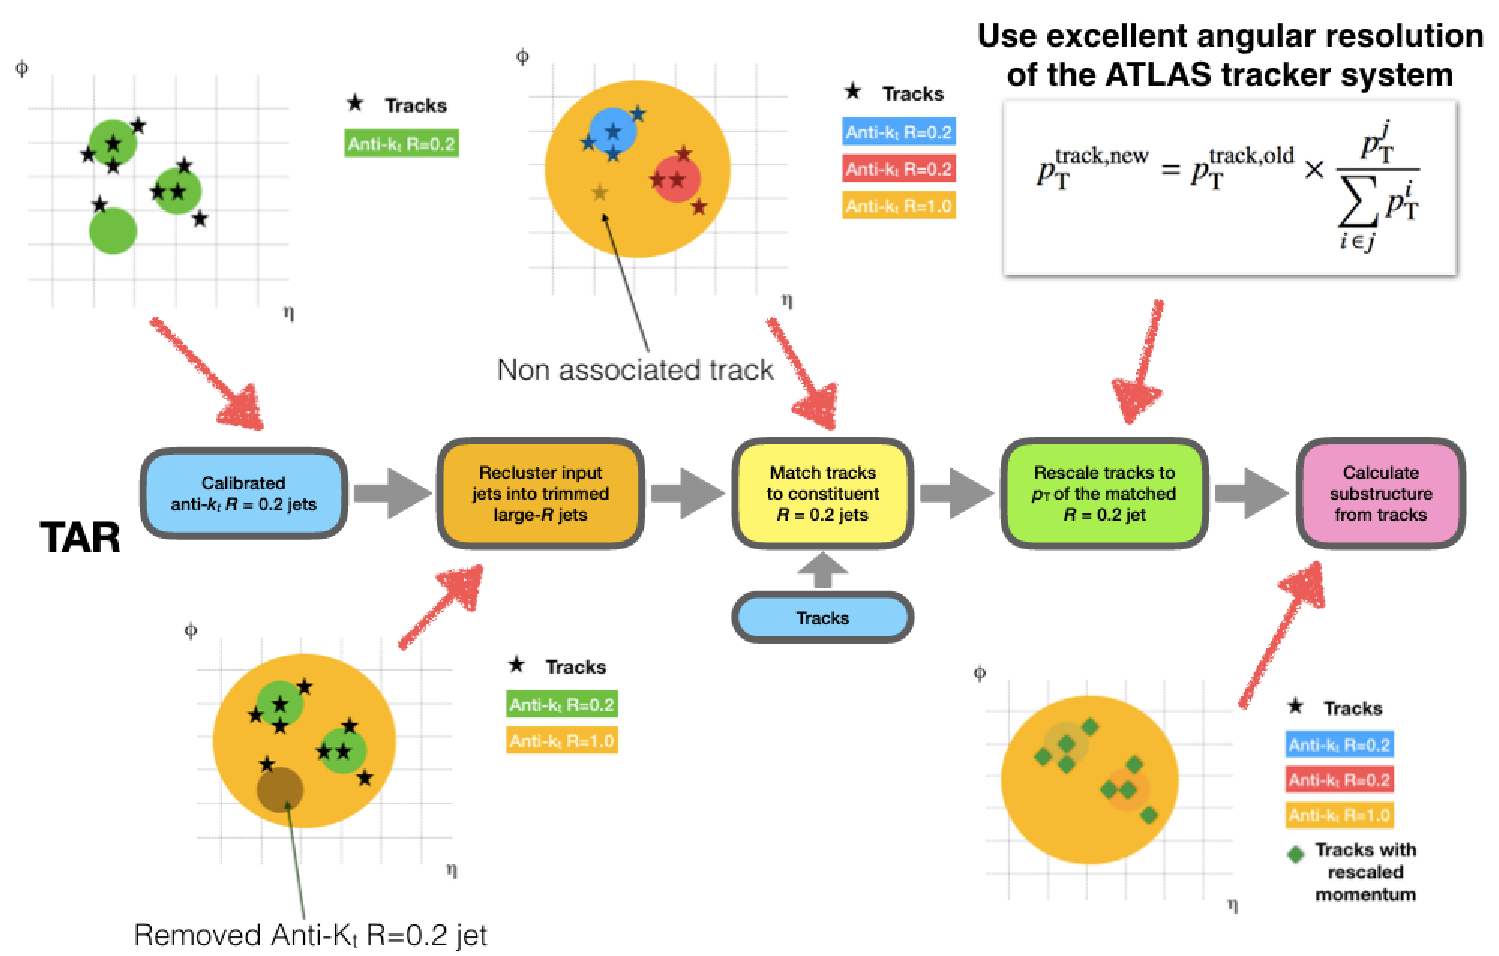
\includegraphics[width = 0.80\textwidth]{Figures/5/TARJetdescription.pdf}
     \caption[TAR jet reconstruction algorithm depicted without lepton disentanglement.]{TAR jet reconstruction algorithm depicted without lepton disentanglement. Figure adapted from \(\copyright\) \cite{TAR_algo}}
     \label{fig:TARAlg}
  \end{figure}

\begin{table}[htbp]
\centering
\caption{TAR jet reconstruction parameters.}
\label{tab:TARparameters}
\begin{tabular}{l l }
\toprule
\multirow{3}{*}{Track selection} & \verb|Loose| quality\\
	& \(\pt > 0.5~\GeV\) \\
	& \(|\eta| < 2.5\)  \\
Tracks removed if associated to & electrons, muons \\
\midrule
\multirow{3}{*}{Input jet selection} & \(R=0.2\) \akt jets \\
	& \(\pt > 20~\GeV\) \\
	&  \(|\eta| < 2.5\)  \\
\midrule
Reclustering radius & \(R=1.0\) \\
TAR jet \pt & \(\pt^\text{TAR} > 100~\GeV\) \\
Trimming radius & \(R=0.2\) \\
Trimming \pt fraction & \(f_\text{cut}=0.05\) \\
Track-to-jet association & \(\DeltaR(\text{jet, track}) < 0.3\) \\
jet-electron overlap removal & \(\DeltaR(\text{jet, electron}) < 0.2\) \\
\bottomrule
\end{tabular}
\end{table}

\subsection{\met}
\label{sec:met_object_description}

The missing transverse momentum \met, introduced in Section \ref{sec:met}, quantifies the imbalance of momentum in the plane transverse to the beam line. In the event that all particles produced in a \(pp\) collision are fully detected, conservation of momentum implies that the transverse momenta of all objects produced by the event should sum to zero within detector resolution. As a result, large \met in an event is indicative of the production of undetected energetic particles. The semileptonic \(s\rightarrow WW(qq\ell\nu)\) decay channel of the LHC signature for the DH model probed in this DM search (see Chapter \ref{chapter:dh_model} for details) predicts large (i.e. above-detector-resolution) \met in the final state. The large \met would be due both to the DM pair produced from the decay of the hypothetical \Zprime, and to the neutrino produced by the leptonic decay of one of the \(W\) bosons in the final state. Both the DM pair and the neutrino would be expected to pass through the detector without any appreciable interactions due to their very low interaction cross sections with SM particles, and hence constitute undetected (i.e. missing) momentum in the event.

The \met is calculated using fully calibrated and reconstructed physics objects (for details, see Ref. \cite{PERF-2016-07}). For this search, baseline electrons and muons (see \Sect{\ref{sec:charged_leptons}}) and \(R=0.4\) jets (see \Sect{\ref{sec:atk4_jets}}) are used to construct the \met. A soft term is additionally included, which uses tracks that are not associated with any of these reconstructed objects. 
%Reconstructed \(\tau\)-leptons and photons are not considered in the calculation of \met.

This search also makes use of the object-based \met significance \metsig \cite{ATLAS-CONF-2018-038}, which is designed to be positively correlated with the likelihood that the measured \met was actually produced by undetected particles in the event, rather than by fluctuations arising from the limited detector resolution. The \met significance is calculated on an event-by-event basis using the uncertainties associated with the reconstructed objects involved in the \met calculation for the given event.
%, as well as terms for the soft term and a pileup correction.

\subsection{Overlap Removal}

To avoid double-counting any physics objects in an event, a priority-based overlap removal (OR) strategy is employed, which eliminates any overlap between the physics objects. This is accomplished by removing all but the highest-priority object from any region in which objects overlap. The strategy presented in this section resolves any overlap between electrons, muons and \(R=0.4\) \smallR jets. The overlap removal between leptons and TAR jets is described in Section \ref{sec:TAR_algo}. No overlap removal between \(R=0.4\) jets and TAR jets is applied, as they are not used in the same selection (see Section \ref{sec:evt_selections} for details). Table \ref{tab:OR} summarizes the criteria under which overlap is removed between a given pair of objects. 

Overlap removal is performed for baseline objects, and only the remaining objects are considered as candidate signal objects. Note that the calorimeter-tagged (CT) muons listed in Table \ref{tab:OR}, details of which can be found in Section 4 of Ref. \cite{muon_reco}, are identified and reconstructed using only inner detector tracks and calorimeter energy deposits consistent with a minimum-ionizing particle, and do not have any associated hits identified in the muon spectrometer. Due to the absence of any associated signal in the muon spectrometer, these CT muons are given a relatively low priority in the OR procedure compared with non-CT muons, which do activate the muon spectrometer.

\begin{table}[htbp]
\centering
\caption[Object priorities and overlap removal criteria for each pair of physics objects considered in the overlap removal procedure.]{Object priorities and overlap removal criteria for each pair of physics objects considered in the OR procedure. Object pairs and removal criteria are listed in the sequence by which they are considered for OR, with the top row considered first. }
\label{tab:OR}
\small{
\begin{tabular}{l l p{7cm}}
\toprule
\textbf{Removed Object} & \textbf{Retained Object} & \textbf{Criteria for OR} \\
\midrule
\midrule
Electron (lower \pt) & Electron (higher \pt) & shared inner detector track \\
Muon & Electron & shared ID track, and muon is CT \\
Electron & Muon & shared ID track, and muon is not CT \\
\akt4 Jet & Electron & Angular separation \(\DeltaR < 0.2\) \\
Electron & \akt4 Jet & \(\DeltaR < \min{(0.4, 0.04 + 10~\GeV / \pt(e))}\) \\
\akt4 Jet & Muon & fewer than 3 tracks in jet, and (muon is ghost-associated to jet, or \(\DeltaR < 0.2\)) \\
Muon & \akt4 Jet & \(\DeltaR < \min{(0.4, 0.04 + 10~\GeV / \pt(\mu))}\) \\
\bottomrule
\end{tabular}}
\end{table}

\subsection{Dark Higgs Candidate Mass}
\label{sec:minms}

In principle, the four-momentum of the Dark Higgs boson \(s\) in the DH signal model is simply the sum of the four-momenta of the \(WW\) pair that it decays to:

\begin{equation}
\label{eq:dh_4momentum}
\mathbf{p}_{s} = \mathbf{p}_{W_\text{had}} + \mathbf{p}_{W_\text{lep}}
\end{equation}

\noindent where \(W_\text{had}\) (\(W_\text{lep}\)) denotes the hadronically (leptonically) decaying \(W\) boson. The \(W_\text{had}\) four-momentum is reconstructed in the resolved regime using the pair of \akt4 jets whose invariant mass is closest to the on-shell \(W\) mass of \(80.4~\GeV\) (see Section \ref{sec:resolved_w_cand}), or in the merged regime as the four-momentum of the highest-\pt \(R=1.0\) TAR jet (see Section \ref{sec:TAR_jets}). The four-momentum of the \(W_\text{lep}\) is the sum of four momenta of its lepton and neutrino daughters:

\begin{equation}
\label{eq:Wlep_4momentum}
\mathbf{p}_{W_\text{lep}} = \mathbf{p}_\ell + \mathbf{p}_\nu
\end{equation}

If the neutrino were the only anticipated source of ``true \met" (i.e. \met arising from undetected particles rather than limited detector resolution) in the final state, the final state \met could be unambiguously assigned to the neutrino, i.e. (\(p_{x,\nu}, p_{y,\nu}) = (E_x^\text{miss}, E_y^\text{miss})\), at which point the only missing information would be the z-component \(p_{\nu,z}\) of the neutrino momentum. However, since the DH signal model additionally predicts  \met originating from the DM pair in the final state, there is some ambiguity involved with assessing how much of the measured \met is accounted for by the neutrino vs. the DM pair.

An approximate solution is obtained by determining the minimum \ms that would be required in order for the \(s\) decay to have produced a lepton and \(W_\text{had}\) with the observed momenta, subject to the constraint that the invariant mass of the reconstructed \(m_{W_\text{lep}}\) be equal to the on-shell \(W\) mass of \(80.4~\GeV\). Although this minimum \ms may not necessarily evaluate to the actual modelled \ms, by providing an absolute lower bound on the possible range of \ms that could produce the observed final state, it is expected to at least be positively correlated with the actual modelled \ms.

% the lower the mass of a mediator, the larger is the range of mediator momenta for which the decay of the mediator can produce a given final state for which the momentum of one of the final-state particles (the neutrino) is unknown. Therefore, for a given final state, the lowest mediator mass that can kinematically produce the final state has the largest space of momenta available by which it could do so compared with larger candidate mediator masses, and hence the highest likelihood of being the actual mediator mass.

To simplify the math involved in determining the minimum \ms, the coordinate system is rotated without loss of generality such that the lepton is strictly traveling along the \(z\) axis, and the hadronically decaying \(W\) boson \(W_\text{had}\) is in the \(xz\) plane, as shown in Figure \ref{fig:minms_coords}.

\begin{figure}[H]
  \centering
     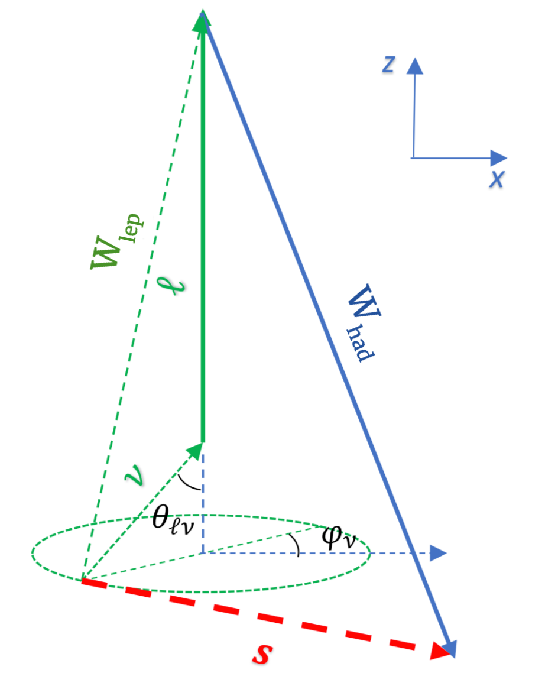
\includegraphics[width = 0.4\textwidth]{Figures/5/minms_coords.pdf}
     \caption[Coordinate system used to evaluate the DH candidate mass \minms.]{Coordinate system used to evaluate the minimum DH mass \ms that is kinematically required to produce the observed final state, subject to the constraint that \(m_{W_\text{lep}} = 80.4~\GeV\).}
     \label{fig:minms_coords}
  \end{figure}
  
In this rotated coordinate system, the four-momenta \(\mathbf{p}_\nu\), \(\mathbf{p}_\ell\) of the neutrino, lepton and hadronically decaying \(W\) boson, respectively, are given by:

\begin{equation}
\label{eq:neutrino_momentum}
\mathbf{p}_\nu = E_\nu(\sin\theta_{\ell\nu}\cos\phi_\nu, \sin\theta_{\ell\nu}\sin\phi_\nu, \cos\theta_{\ell\nu}, 1)
\end{equation}

\begin{equation}
\label{eq:lepton_momentum}
\mathbf{p}_\ell = E_\ell(1, 0, 0, 1)
\end{equation}

\noindent and 

\begin{equation}
\label{eq:lepton_momentum}
\mathbf{p}_{W_\text{had}} = (E_{W_\text{had}}, p_{W_\text{had}, x}, 0, p_{W_\text{had}, z})
\end{equation}

\noindent where \(\theta_{\ell\nu}\) is the angular separation between the lepton and the neutrino, and \(\phi_\nu\) is the angle of the neutrino relative to the \(x\) axis in the \(xy\) plane. The \ms is then obtained by squaring the four-momenta in Eq. \ref{eq:dh_4momentum}:

\begin{multline}
\label{eq:ms_squared}
\ms^2 = (\mathbf{p}_{W_\text{had}} + \mathbf{p}_{W_\text{lep}})^2 = (\mathbf{p}_{W_\text{had}} + \mathbf{p}_\ell + \mathbf{p}_\nu)^2 \\
= (E_{W_\text{had}} + E_\ell + E_{\nu})^2 - (p_{W_\text{had}, x} + E_{\nu}\sin \theta_{\ell\nu}\cos \phi_{\nu})^2 - (E_{\nu}\sin \theta_{\ell\nu}\sin \phi_{\nu})^2 - (E_\ell + p_{W_\text{had}, z} + E_{\nu}\cos \theta_{\ell\nu})^2
\end{multline}

\noindent It can be shown by taking derivatives of Eq. \ref{eq:ms_squared} that the minimum \ms occurs when \(\phi_v=0\) (i.e. when the neutrino is in the same plane as the \(\mathbf{p}_{W_\text{had}}\)).


Setting \(\phi_v=0\) in Eq. \ref{eq:ms_squared} and using the Pythagorean identity \(\sin \theta = \sqrt{1-\cos^2\theta}\):

\begin{multline}
\label{eq:ms_squared_simplified}
m_s^2 = \left(E_\ell + E_\nu + E_{W_\text{had}}\right)^2 - \left(p_{W_\text{had}, x}  + E_\nu\sqrt{1 - \cos^2\theta_{\ell\nu}}\right)^2 \\ - \left(E_\ell + p_{W_\text{had}, z}\cos \theta_{Wl} + E_\nu\cos \theta_{\ell\nu} \right)^2
\end{multline}

This leaves an equation for \ms with two unknowns: the energy \(E_\nu\) of the neutrino, and the cosine \(\cos\theta_{\ell\nu}\) of the angle between the lepton and the neutrino. The neutrino energy is determined as a function of \(\cos\theta_{\ell\nu}\), by imposing the constraint that the mass \(m_{W_\text{lep}}\) of the leptonically decaying \(W\) boson be set to the on-shell \(W\) boson mass of \(m_W=80.4~\GeV\):

\begin{equation}
\label{eq:Ev}
m_{W_\text{lep}}^2 = m_W = (p_\ell + p_{\nu})^2 = 2p_\ell p_{\nu} = 2E_\ell E_{\nu}(1 - \cos\ \theta_{\ell\nu})\\
\end{equation}

\noindent Solving for \(E_\nu\):

\begin{equation}
\label{eq:Ev_solved}
E_{\nu} = \frac{m_W^2}{2E_\ell(1 - \cos\ \theta_{\ell\nu})}
\end{equation}

With this independent determination of \(E_\nu\), the minimum \ms in Eq. \ref{eq:ms_squared_simplified} is evaluated numerically by scanning over \(\cos\ \theta_{\ell\nu} \in [-1,1]\) and identifying the value of \(\cos\ \theta_{\ell\nu}\) that minimizes \ms (excluding \(\cos\ \theta_{\ell\nu}=1\) to avoid a singularity in Eq. \ref{eq:Ev_solved}).

Figure \ref{fig:minms_reco} shows distributions of this minimized ``\minms" for MC simulated events produced with the DH signal model over a range of \ms (left column) or \mZp (right column). The distributions are more sharply peaked for lower \ms, and for higher \ms the location of peak in \minms becomes increasingly shifted to the left of (i.e. below) the actual modelled \ms. The minimal variation between the different modelled values of \mZp presented in distributions in the right-hand column of Figure \ref{fig:minms_reco}, which scan over a range of \mZp for the same \ms, offers an encouraging indication that the value of the \minms variable is primarily a function of the \ms parameter in the model that it is designed to approximate.

Despite the shifted location of the peaks at higher \ms, the presence of distinct peaks in the approximate vicinity of the modelled \ms imply that the \minms variable can be a valuable tool to aid in discriminating events in the data that could be consistent with the DH signal process from the SM background processes. For this reason, events in the signal regions are binned in \ms when searching for evidence of the signal model in the ATLAS collision data. The binning in \minms is presented in detail in Section \ref{sec:binning_strategy}.

\begin{figure}[H]
	\centering
	\begin{subfigure}[b]{0.49\textwidth}
	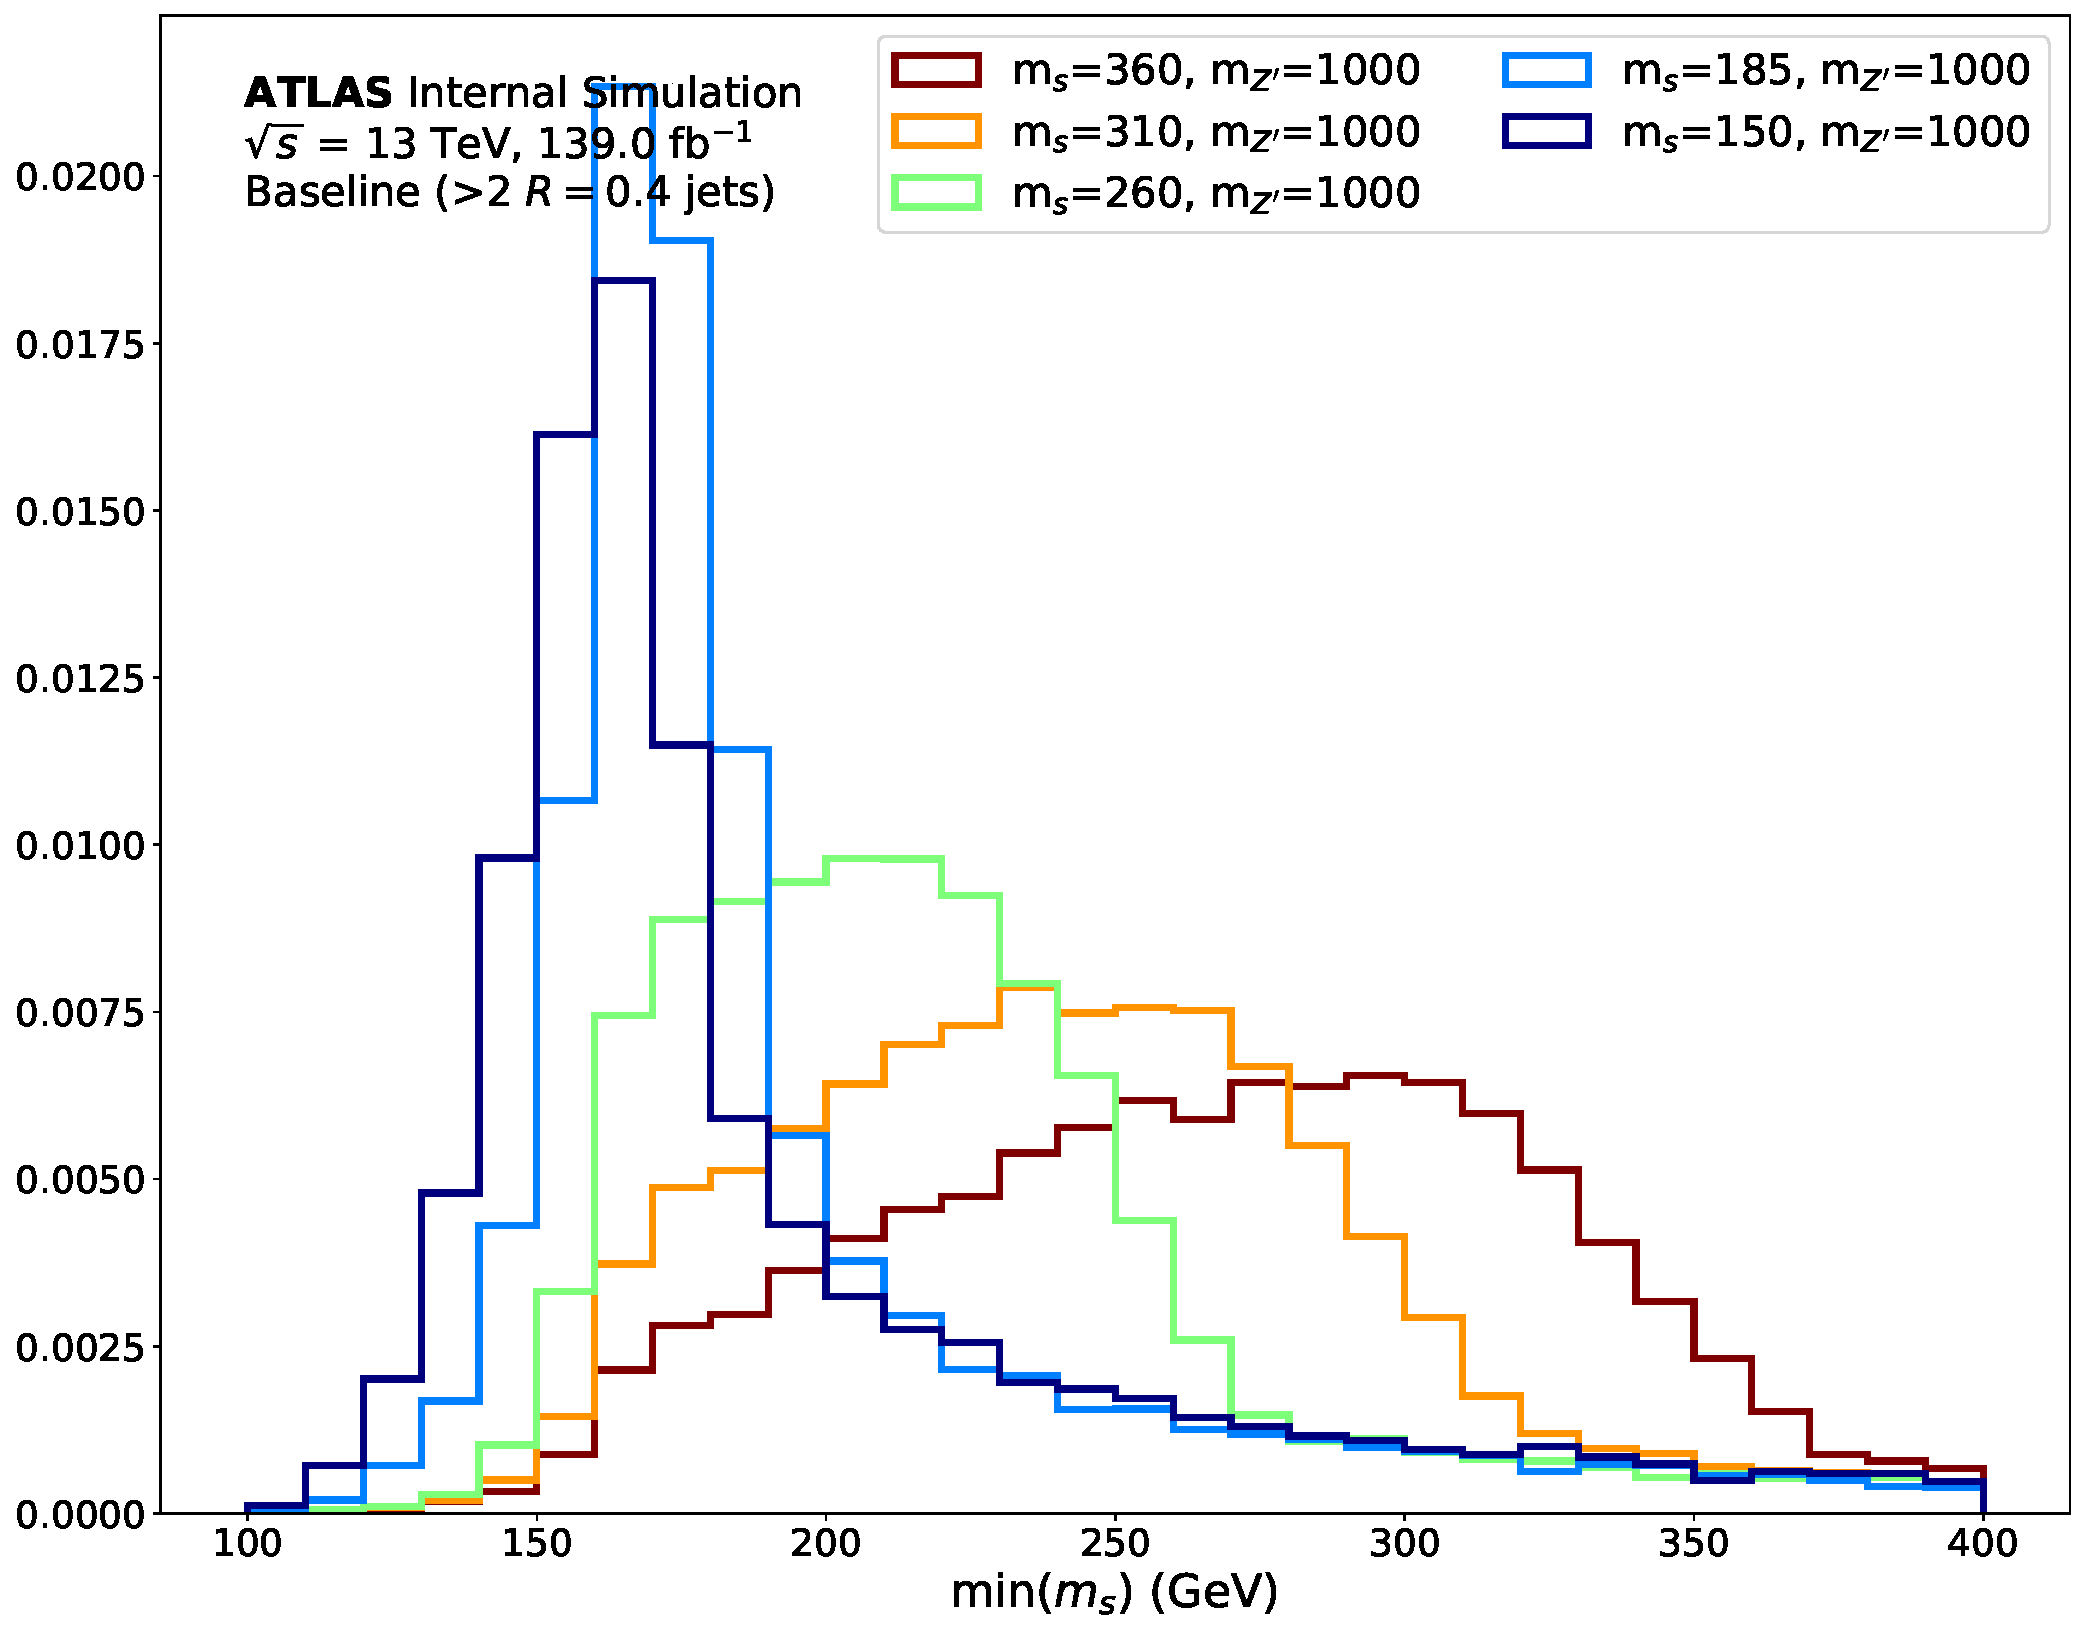
\includegraphics[width=0.95\textwidth]{Figures/5/TARJets10_minmS_res_ms.pdf}
	\caption{\mZp fixed, \ms varied}
	\label{fig:minms_res_ms}
	\end{subfigure}
	\begin{subfigure}[b]{0.49\textwidth}
	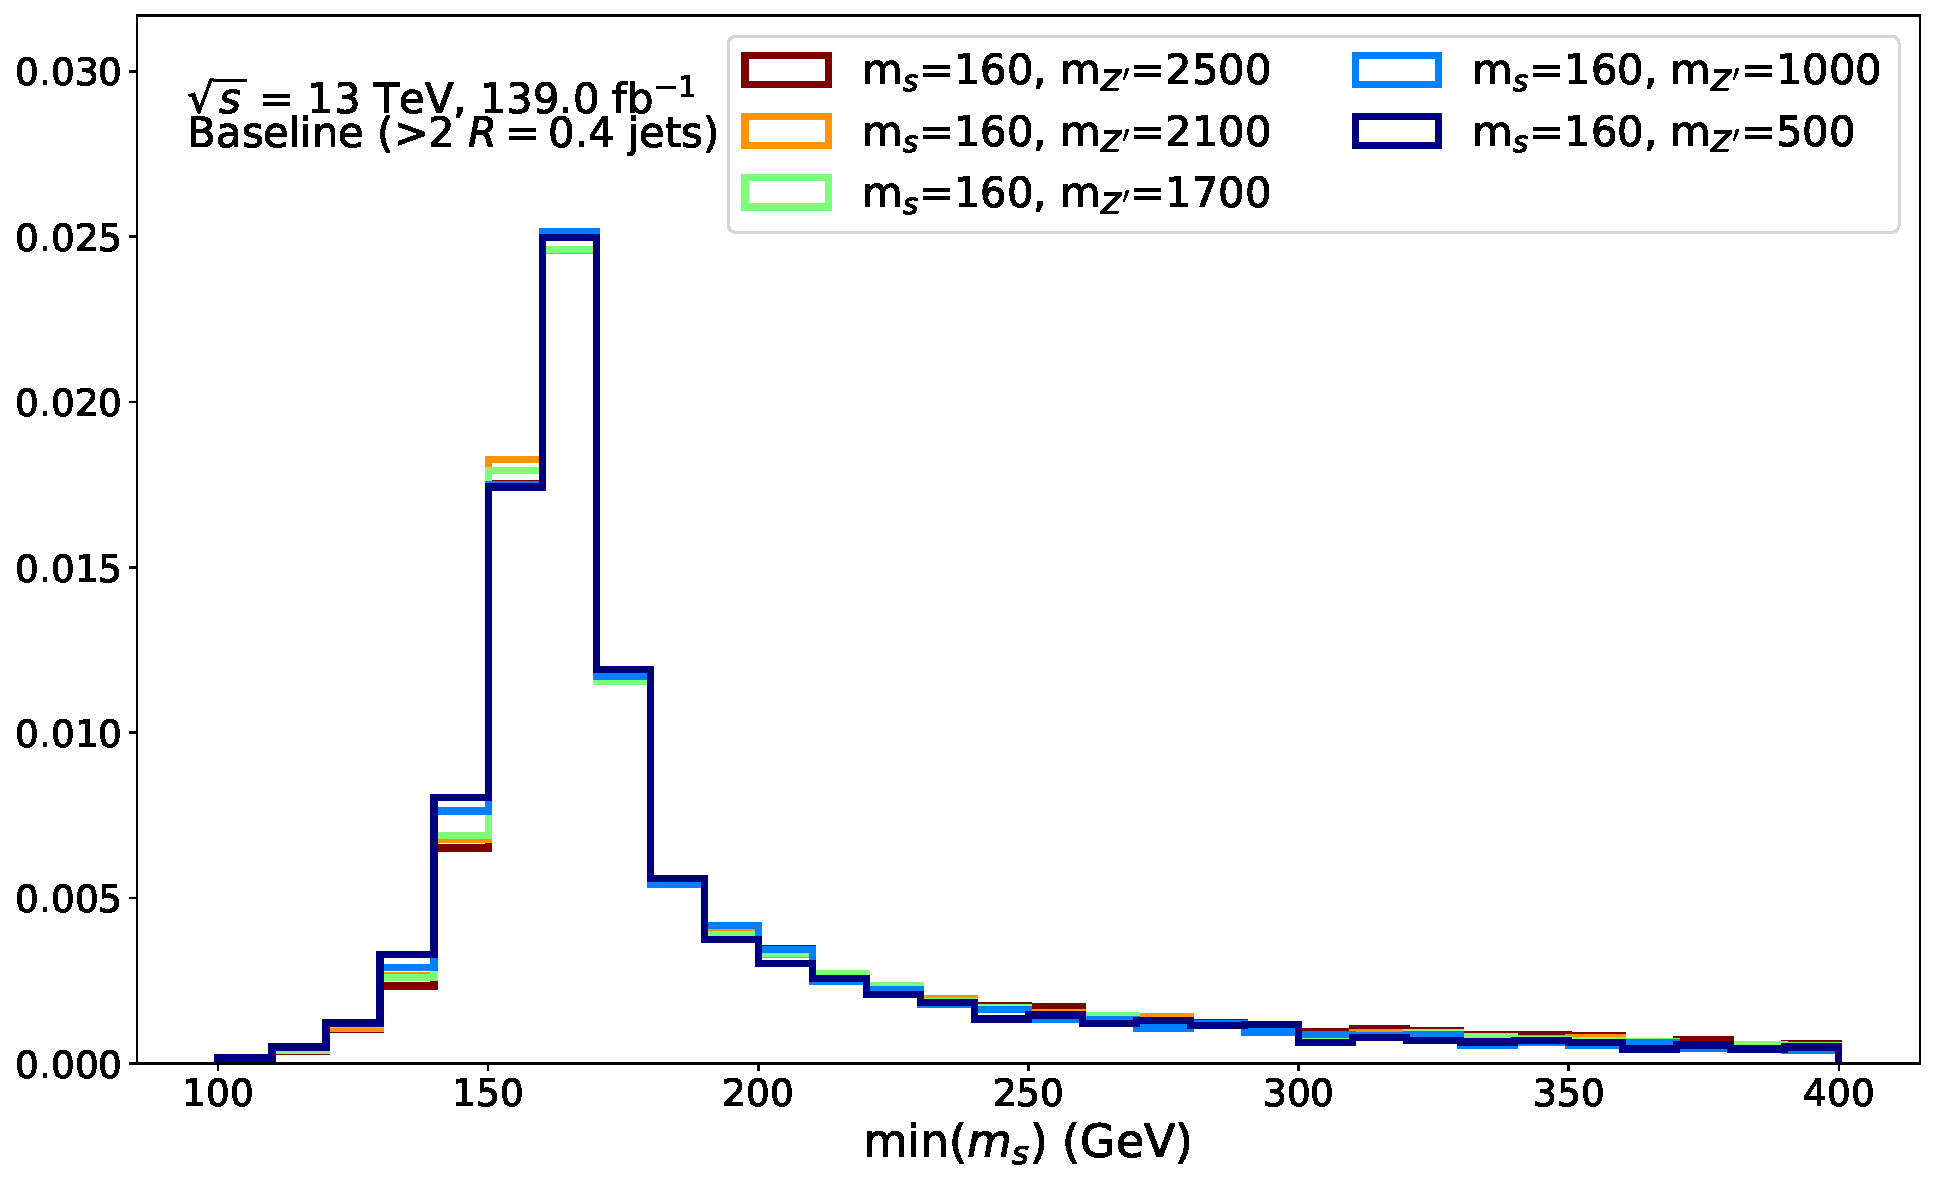
\includegraphics[width=0.95\textwidth]{Figures/5/TARJets10_minmS_res_mZp.pdf}
	\caption{\ms fixed, \mZp varied}
	\label{fig:minms_res_mZp}
	\end{subfigure}
	\begin{subfigure}[b]{0.49\textwidth}
	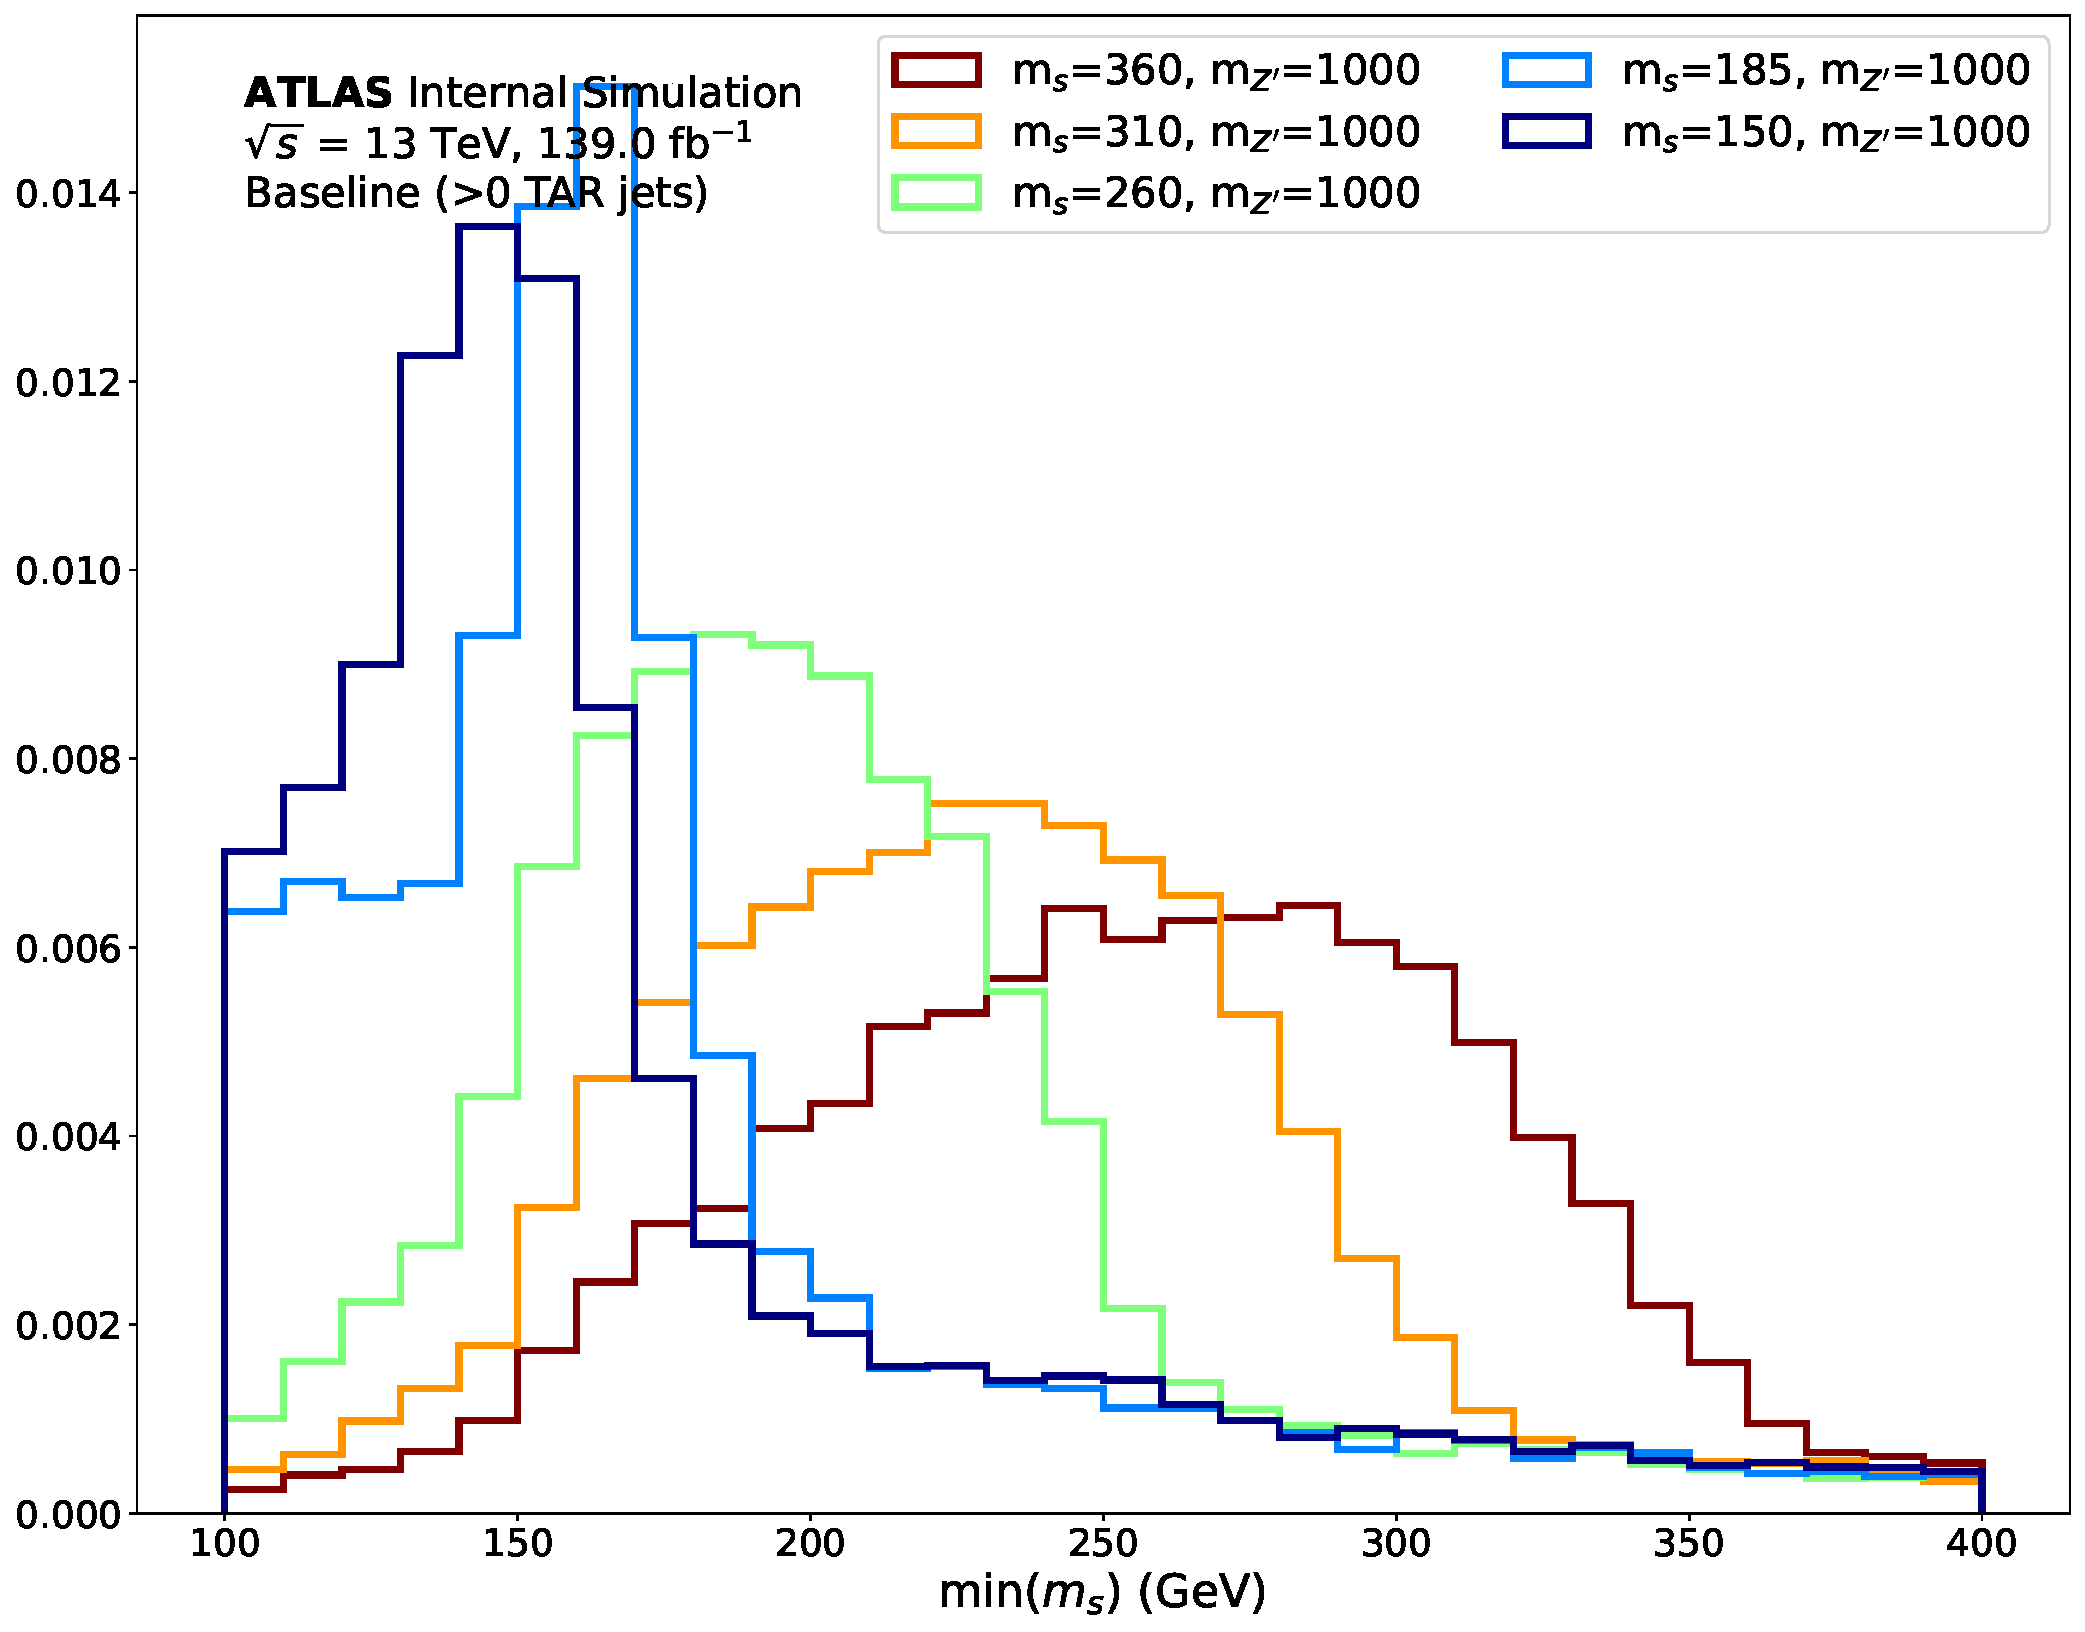
\includegraphics[width=0.95\textwidth]{Figures/5/TARJets10_minmS_mgd_ms.pdf}
	\caption{\mZp fixed, \ms varied}
	\label{fig:minms_res_ms}
	\end{subfigure}
	\begin{subfigure}[b]{0.49\textwidth}
	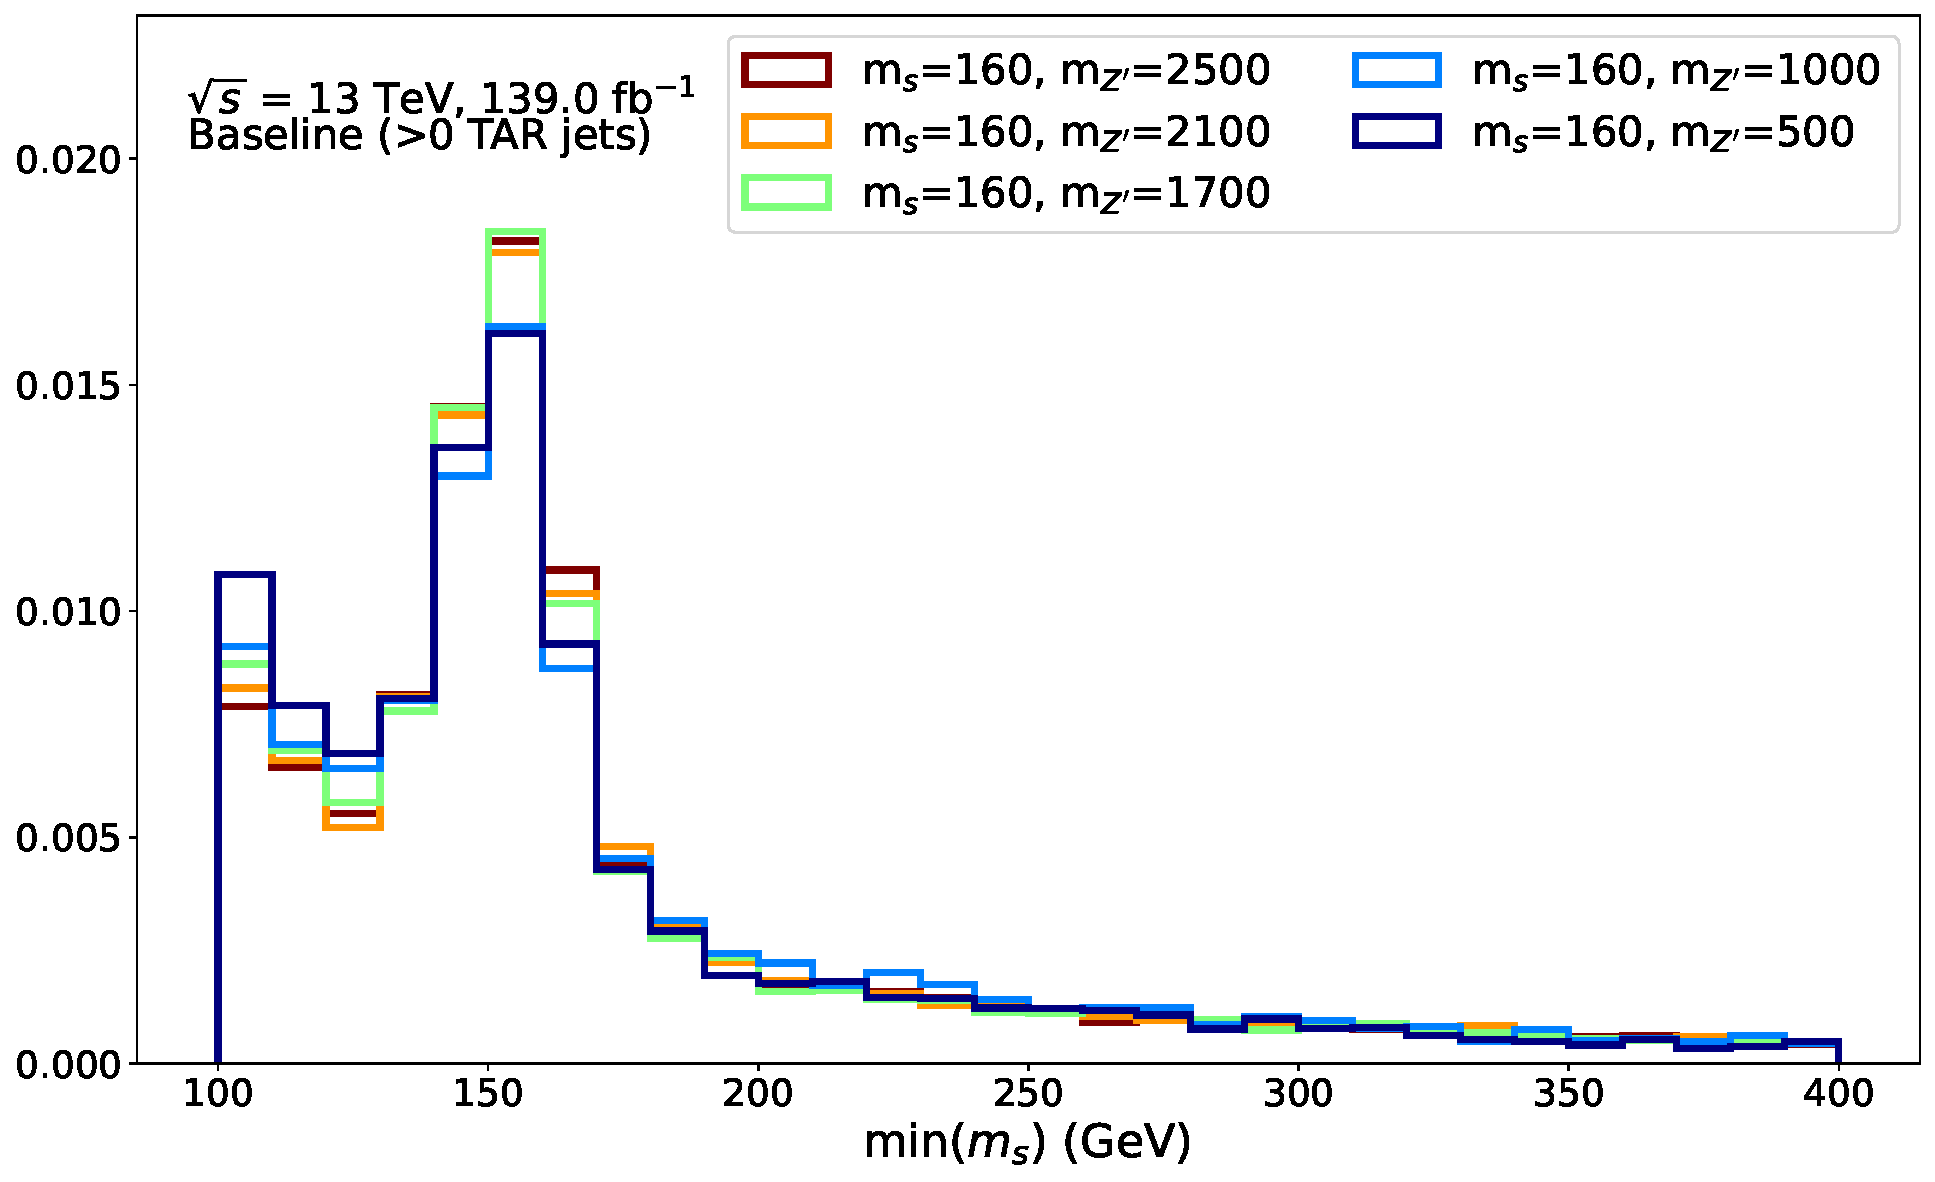
\includegraphics[width=0.95\textwidth]{Figures/5/TARJets10_minmS_mgd_mZp.pdf}
	\caption{\ms fixed, \mZp varied}
	\label{fig:minms_res_mZp}
	\end{subfigure}
	\caption[Distributions of the DH candidate mass \minms for MC simulated events produced for the DH signal model over a range of \ms and \mZp.]{Distributions of the DH candidate mass \minms, reconstructed using the minimization strategy presented in Section \ref{sec:minms}, for MC simulated events produced for the DH signal model over a range of \ms and \mZp. Distributions are normalized to unit area. Events included in all distributions are required to pass the baseline selection requirements presented in Section \ref{sec:evt_selections}. For the distributions shown in the top (bottom) row, the \(W_\text{had}\) is reconstructed as a resolved candidate (TAR jet) using the strategy presented in Section \ref{sec:resolved_w_cand} (\ref{sec:TAR_algo}), and events are required to have \(\geq2\) \(R=0.4\) \smallR jets (\(\geq1\) \(R=1.0\) TAR jets) reconstructed in the final state.}
	\label{fig:minms_reco}
\end{figure}

\subsection{Transverse Mass}
\label{sec:transverse_mass}

The transverse mass \(m_T(\met, \ell)\) between the lepton and \met is considered in this search because it is sensitive to the presence of additional \met beyond that arising from the neutrino in the leptonic decay of the \(W_\text{lep}\). It is computed for events measured in the ATLAS detector as:

\begin{equation}
\label{eq:mtlepmet_atlas}
m_T(\ell, \met) = \sqrt{2p_{T, \ell} \met(1-\cos\theta_{\ell, \met})}
\end{equation}


\noindent which is derived from the more general transverse mass definition found in Section 49.6.1 of Ref. \cite{pdg_2020}.

\begin{multline}
\label{eq:mtlepmet_full}
m_{T, \text{ full}}^2(\ell, \met) = (E_{T, \ell}^2 + E_{T, \met}^2 - (p_{T, \ell}^2 + p_{T, \met}^2)) \\
= m_\ell^2+m_{\met}^2 + 2E_{T, \ell}, E_{T, \met}(1-\cos\theta_{\ell, \met})
\end{multline}

\noindent under the assumptions that the masses associated with the lepton and \met are negligibly small compared with their momenta. The assumption of negligible lepton mass is in general justified given the high energy of the \(pp\) collisions at the LHC. The assumption of negligible mass associated with \met is justified if the true \met arises only from the neutrino in the leptonic \(W_\text{lep}\) decay, as it would in the leading SM backgrounds. In the signal model, however, there is additional mass associated with the \met, which arises from the decay of the massive \Zprime mediator to an invisible DM pair. The result, shown in figure \ref{fig:mT_lep_met} after applying the baseline selection, is that the bulk of the SM background has \mtlepmet below the W mass peak, but the signal distribution tends to be peaked closer to \(\sim 250~\GeV\). 

\begin{figure}[H]
	\centering
	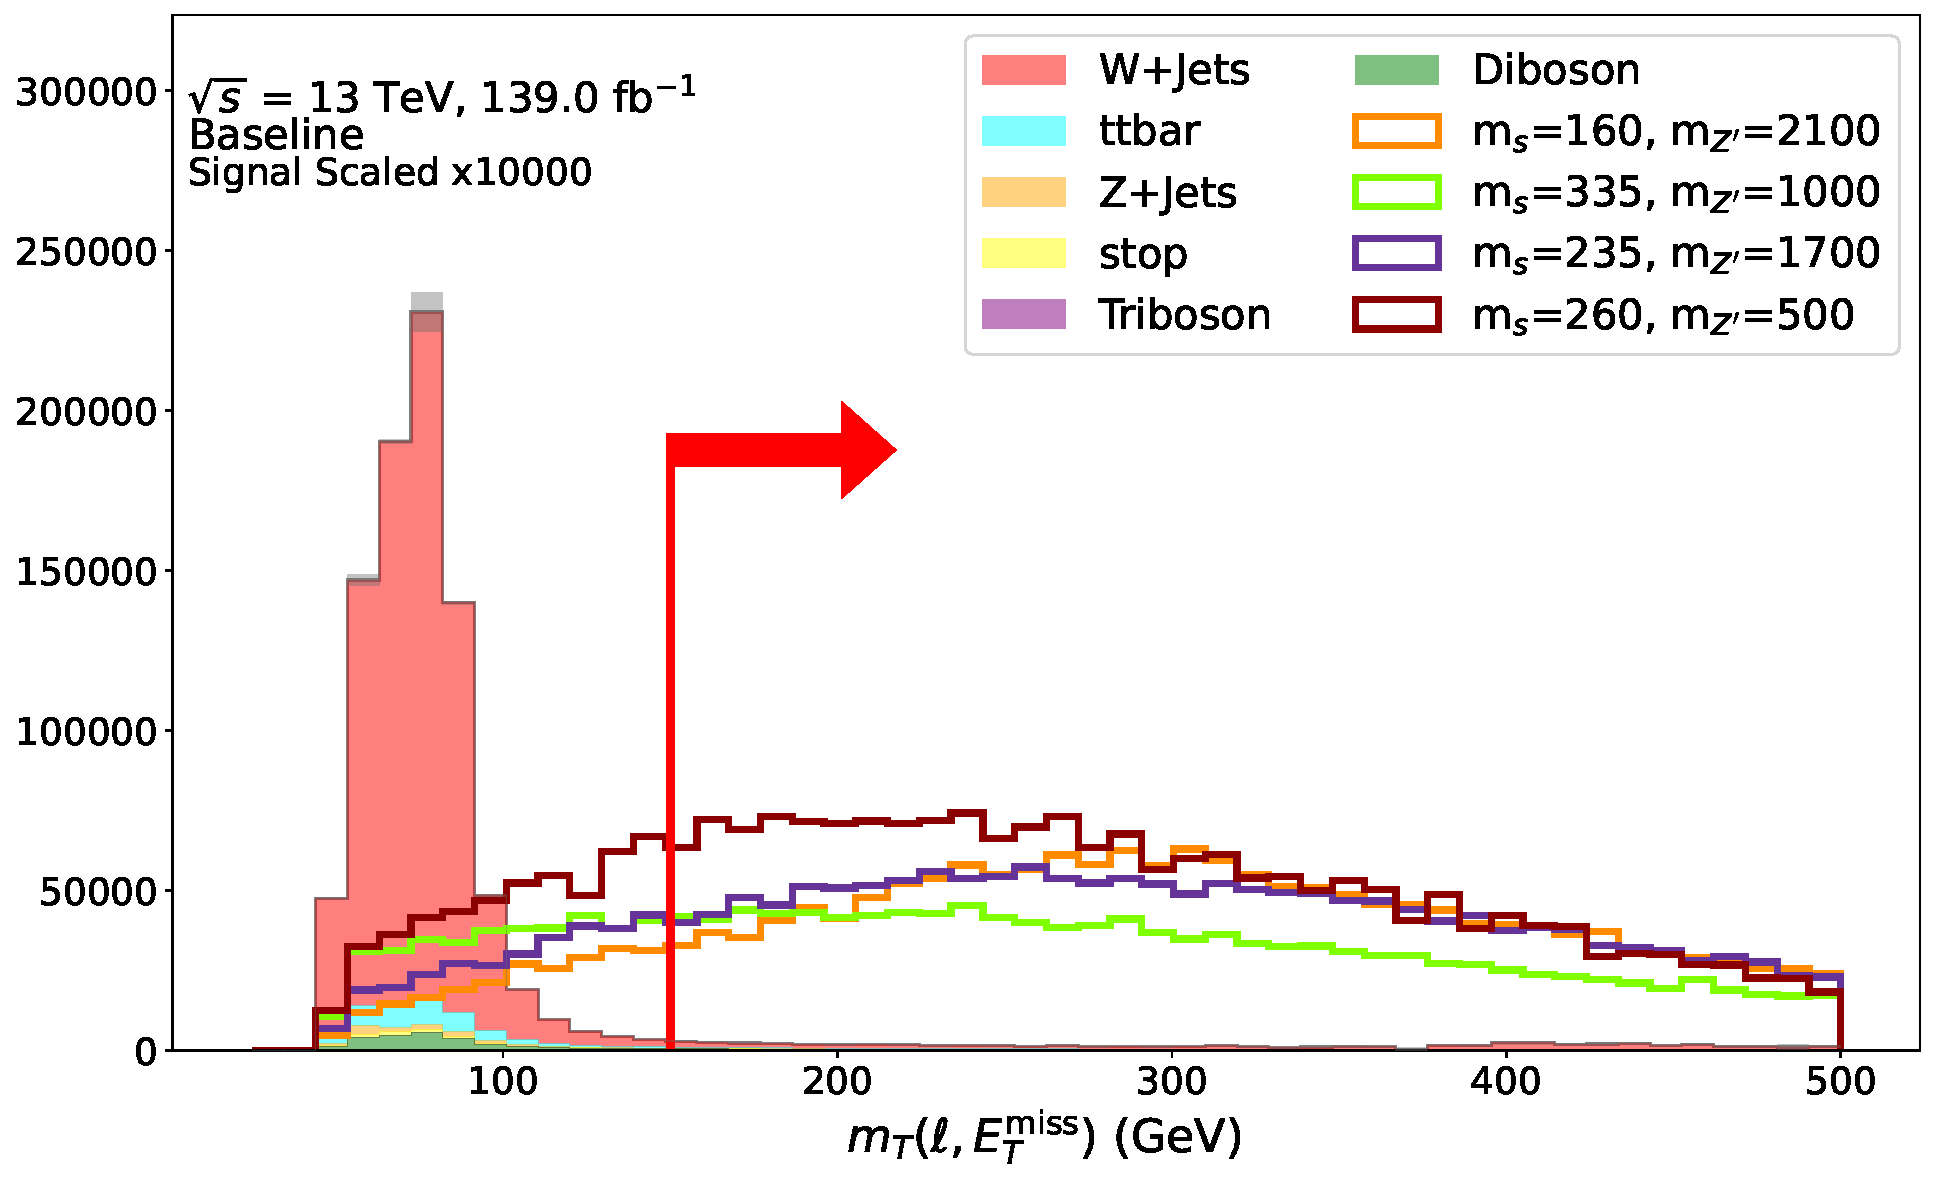
\includegraphics[width=0.7\textwidth]{Figures/5/mT_lep_met_N_1.pdf}
	\caption[Transverse mass distribution for SM background and several signal points,]{Transverse mass distribution for SM background and several signal points with baseline selections, excluding the lower bound on \mtlepmet. The red line and arrow indicate the placement of the baseline selection on \mtlepmet.}
	\label{fig:mT_lep_met}
\end{figure}

\section{Event Selections}
\label{sec:evt_selections}

Selections are applied to the ATLAS collision data and MC simulated events with the aim of defining subsets, or ``regions" of data that are enriched in a particular process of interest for the search. The regions are designed and optimized using MC simulated data (see Chapter \ref{chapter:mc} for a detailed discussion of MC simulation and its application to simulating data produced by the ATLAS detector). The use of MC simulated data makes it possible to quantify the relative contribution to the expected yield of events in the region arising from each physics process predicted in the data.

Selections that define the ``signal regions" (SRs) are optimized to produce an enriched yield of MC simulated events produced using the DH signal model (referred to as ``signal events"), with a minimal yield of simulated events generated to model SM background processes (referred to as ``background events"). A discrepancy between the ATLAS collision data and the predicted yield of SM backgrounds in the signal regions would indicate the presence of a BSM physics process with a production mechanism at the LHC consistent with that of the signal model. ``Control regions" (CRs) are optimized to have an enriched yield of MC simulated events modelled by one particular SM background process. \wjets and \ttbar CRs are defined for this DM search to obtain data-driven constraints on the total yields of these SM background processes in the signal region. 

\subsection{Kinematic Categories}
\label{sec:kin_categories}

Within each of the SRs and CRs, the analysis selection is divided into two kinematic regimes, referred to as ``categories". The ``merged" category is designed to target the merged regime discussed in Section \ref{sec:TAR_jets} in which the hadronic decay products are sufficiently boosted as to be reconstructed as a single \(R=1.0\) TAR jet. The leading \pt TAR jet is then used to reconstruct the candidate hadronically decaying \(W\) boson \(W_\text{had}\) in the signal model. The ``resolved" category targets the lower-\pt regime in which the hadronic decay products have a sufficient angular separation that they cannot be reclustered into a TAR jet, and are instead reconstructed as resolved \smallR \akt \(R=0.4\) jets. As described in Section \ref{sec:resolved_w_cand}, the \(W_\text{had}\) is reconstructed in the resolved category using the two \smallR jets whose combined invariant mass is nearest to \(m_W=80.4~\GeV\).

\Fig{\ref{fig:categories}} illustrates the two kinematic categories.

\begin{figure}[htbp]
	\centering
	\begin{subfigure}[t]{0.45\textwidth}
	\centering
	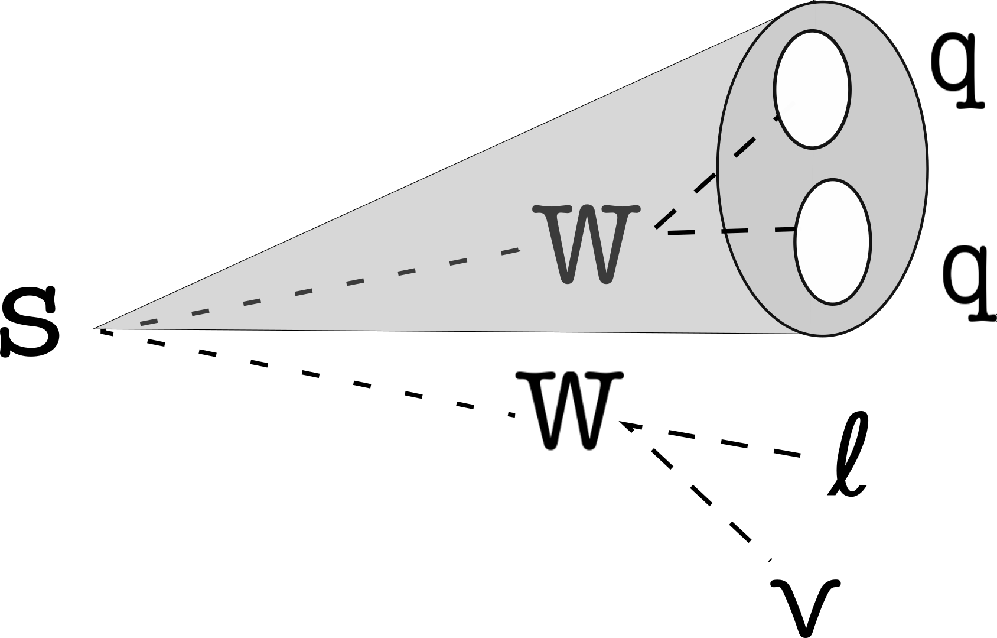
\includegraphics[width=0.75\textwidth]{Figures/5/merged.pdf}
	\end{subfigure}
	\begin{subfigure}[t]{.45\textwidth}
	\centering
	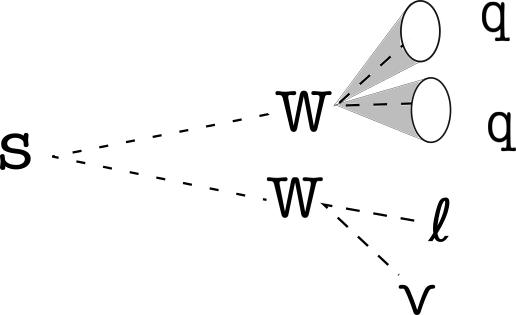
\includegraphics[width=0.75\textwidth]{Figures/5/resolved.png}
	\end{subfigure}
	\caption[A graphical representation of the two kinematic categories used in the search based on the characteristics of the final state.]{A graphical representation of the two kinematic categories used in the search based on the characteristics of the final state. Left: merged category, in which the jets produced by the \(w\rightarrow q\bar{q}\) are sufficiently boosted as to be reconstructed within a single \largeR TAR jet. Right: resolved category, in which the two quarks are reconstructed separately as two \smallR \akt \(R=0.4\) jets.}
	\label{fig:categories}
\end{figure}

Within each of the signal and control regions, the selection is divided into the merged and resolved kinematic categories presented in Section \ref{sec:kin_categories}. Events are classified into the merged category if there is at least one reconstructed \(R=1.0\) TAR jet in the final state (\(\NTAR > 0\)), and the resolved category if there are at least two reconstructed \(R=0.4\) \smallR jets (\(\Njets > 1\)). Selections are further refined and optimized separately within each category. It is worth noting that, as is, the requirements for events to be classified into the merged or resolved categories are not mutually exclusive - i.e. there are events that have least one \(R=1.0\) TAR jet \textbf{and} at least two \smallR jets. To avoid double-counting the same events in the search, orthogonality between the merged and resolved categories is therefore enforced in all of the signal and control regions by explicitly requiring events that pass the requirements to be classified into the resolved category in any region to have additionally failed the merged category selection in all regions.  

\subsection{Baseline selection}
\label{ap:preselection}

The baseline preselection is common to all analysis regions and categories used in the search, and is used to roughly define the region of interest for the search prior to any detailed optimization of selection requirements or sub-division into separate analysis regions. The baseline selection is defined as follows:

\begin{itemize}
\item (1 signal muon or 1 signal electron) and no additional baseline muons or electrons
\item (\met trigger passed) OR ( (single muon trigger passed) AND (signal muon matched to muon trigger) )
\item \(\met > 200~\GeV\)
\item \(\metsig > 5\)
\item \(\mtlepmet > 150~\GeV\)
%\item veto on b-tagged \smallR (\(R=0.4\)) jets (a.k.a. \bjet veto)
\item \(\NTAR > 0\) or \(\Njets > 1\)
\end{itemize}

See Section \ref{sec:charged_leptons} for the definitions of baseline and signal muons and electrons, and Section \ref{sec:triggers_evt_selection} for details of the \met and single muon triggers as well as the single muon trigger matching requirement. The veto on baseline muons or electrons in addition to requirement of a single signal lepton is designed to improve the purity of the single lepton final state predicted by the signal model by removing events in which an additional lepton was produced from the hard scatter and reconstructed as a baseline lepton, yet failed the criteria to be identified as a signal lepton. 


\subsection{Signal Region Definition}
\label{sec:sr_selection}

In addition to the baseline selection, a veto on jets identified as having been induced by a \(b\) quark (a.k.a. a \bjet veto) is applied in the SR to reduce the yield of SM \ttbar and single-top processes discussed in Section \ref{sec:SM_bkg_sim}. See Section \ref{sec:btag} for details of the \bjet tagging algorithm. 


Within each category, the baseline selection is further refined by optimizing the exact placements of upper or lower bounds, also referred to as ``cuts", on variables for which the distributions of MC simulated events generated according to the signal model differs appreciably from MC simulated distributions of the SM background processes.

Broadly, the cut placements are optimized to maximize the predicted yield of MC simulated events that model the DH signal process relative to the predicted yield of events that model the SM background processes. However, this basic benchmark fails to account for the fact that, as discussed in Section \ref{sec:mc_intro}, the relative ``statistical uncertainty" associated with the limited number of MC simulated events used to calculate yield predictions will increase as the selections are tightened (i.e. as lower bounds are increased or upper bounds are reduced) due to the resulting reduction in the number of MC simulated events that pass the selections. As the relative statistical uncertainty of the predicted yields increases, the ability of the search to confidently identify an excess of ATLAS collision events above the predicted yield of SM background processes - which would be indicative of additional events produced by a BSM process - is reduced. Furthermore, as the predicted yield of events is reduced, the relative statistical uncertainty associated with the number of observed events, derived from the Poisson distribution, will also increase and similarly impact the sensitivity of the search. Therefore, while if is often valuable to tighten certain selections in order to increase the relative predicted yield of the signal process, it is also important to avoid over-tightening them to the point that the statistical uncertainty of the predicted and observed event yields begins to reduce the sensitivity of the search. 

A metric known as the ``Asimov discovery significance" \cite{Buttinger:2643488} \(Z\) is used as a means of quantifying the sensitivity of a signal region given the predicted yields \(s\) and \(b\) of the signal and background processes, respectively, while also accounting for the statistical uncertainty \(\sigma_b\) associated with the limited number of MC simulated events used to predict \(b\):

\begin{equation}
  \label{eq:asimov}
  Z(s, b, \sigma_b) = \left[ 2(s+b)\left(
    \ln\left[ \frac{(s+b)(b+\sigma_b^2)}{b^2 + (s+b)\sigma_b^2} \right]
    - \frac{b^2}{\sigma_b^2}\ln\left[ 1 + \frac{\sigma_b^2 s}{b(b+\sigma_b^2)} \right]
  \right) \right]^\frac{1}{2}
\end{equation}

\subsubsection{Optimization Strategy for Signal Region Definition}
\label{sec:sr_opt}

After applying the baseline selections and \bjet veto, the placement of upper and lower bounds is optimized for the selection variables listed in Table \ref{tab:opt_vars}. The SR was kept ``blinded" during optimization, which means that only the MC simulated signal and background events were considered, and not the ATLAS collision data. Blinding is done in order to avoid biasing the cut choices on the basis of any trends or fluctuations that may be present in the distributions of ATLAS data in the SR.  

The choice of selection variables was made based on a visual assessment of the impact of cuts on all the variables considered as candidate selection variables on the Asimov discovery significance \(Z\). Visualization of \(Z\) with respect to the cut placement on each variable is done using so-called ``N-1" plots, which are shown for the finalized selections in the merged and resolved SRs, respectively, in Figures \ref{fig:Nminus1mergedSR} and \ref{fig:Nminus1resolvedSR}. The N-1 plots are produced for a given variable \(v\) and a given set of candidate selections on all other variables as follows:

\begin{itemize} 
\item Place the candidate selections on all variables except for \(v\).
\item In the upper panel, plot the distributions of the background and signal processes, binned in \(v\).
\item In the lower panel, plot the distributions of the Asimov discovery significance \(Z\) for each signal process plotted in the upper panel.
\begin{itemize}
\item If comparing the placement of an \textbf{upper bound} \(v_u\) on the variable \(v\): calculate the Asimov significance \(Z(v_u)\) for all events with \(v<v_u\): 

\begin{equation}
\label{eq:asimov_upper}
\begin{gathered}
s_u = \sum_{i \in \{\text{signal}, v(i) < v_u\}} w(i) \\
b_u =  \sum_{i \in \{\text{SM backgrounds}, v(i) < v_u\}} w(i) \\
\sigma_{b_u} = \sqrt{ \sum_{i \in \{\text{SM backgrounds}, v(i) < v_u\}} \big[w(i)\big]^2 } \\
\end{gathered}
\end{equation}

\noindent where each event \(i\) is implicitly required to have passed all the other candidate selections for the given process (signal or SM backgrounds) in addition to \((v < v_u)\), and \(w(i)\) is the event weight associated with event \(i\) (see discussion of event weights in Section \ref{sec:evt_weights}). The statistical variance \((\sigma_b)^2\) is evaluated in Eq. \ref{eq:asimov_upper} as the sum of squared weights for events in the background process that pass all other candidate selections in addition to \((v < v_u)\). Inserting \(s_u\), \(b_u\) and \(\sigma_{b_u}\) into Eq. \ref{eq:asimov}:

\begin{equation}
\label{eq:asimov_upper}
Z(v_u) = Z(s_u, b_u, \sigma_{b_u} )
\end{equation}

\item Conversely, if comparing the placement of a \textbf{lower bound} \(v_d\): calculate the Asimov significance \(Z(v_d)\) for all events with \(v>v_d\) by replacing ``\(v<v_u\)" in Eq. \ref{eq:asimov_upper} with ``\(v>v_d\)".
\end{itemize}
\end{itemize}

The optimization was performed first in the merged category of the SR, after placing an additional requirement of at least one \(R=1.0\) TAR jet. Once the selections defining the merged SR were finalized, optimization was subsequently performed in the resolved category, with the \(\NTAR > 0\) requirement replaced by \(\Njets > 1\) in addition to a veto on any events that pass the finalized merged SR selections. 

Since the optimal placement of selections was found to vary to some extent for MC simulated signal data sets with different \ms and \mZp, the cut placements were initially optimized with the aim of maximizing the average Asimov discovery significance for MC simulated data sets at the following four mass points, which cover most of the \ms range considered in the search: (\ms, \mZp) = \{(210, 2100), (285, 1700), (310, 500), (335, 1000)\} GeV. The \mZp values of these four mass points were chosen because they are near the edge of the so-called ``exclusion range", which represents the range of \ms and \mZp within which the search was expected to be sensitive to the presence (or absence) of events produced by the DH signal model in the ATLAS data, at a 95\% confidence level on the basis of sensitivity projections obtained using the method presented in Section \ref{sec:hypo_test} with the Asimov data set. It is particularly desirable to optimize the cut placements for mass points near the edge of the exclusion range in order to extend this range as much as possible. 

An iterative approach was used to optimize cut placements at the four signal points, which combined:

\begin{itemize}
\item repeated grid searches, which scanned over \(1,000,000\) candidate multi-dimensional combinations of cut placements on some or all of the optimized variables to identify combinations that maximized \(Z\), and 
\item visual analysis of N-1 plots such as those shown in Figures \ref{fig:Nminus1mergedSR} and \ref{fig:Nminus1resolvedSR} to visually validate the optimal placements found by the grid searches.
\end{itemize}

It is worth noting that, inspecting Eq. \ref{eq:asimov}, the Asimov discovery significance does not account for the statistical uncertainty \(\sigma_s\) arising from limited MC simulated events in the signal sample. Therefore, in order to ensure sufficient signal region that there were sufficient events in the signal samples, the grid search included an option to avoid cut combinations that reduced the predicted signal yield below some acceptable minimum set by the user. After some testing, it was found that setting a minimum acceptable predicted yield of 15 for the signal point \((\ms, \mZp)=(210, 2100)~\GeV\) was adequate to ensure that the signal samples of interest for cut optimization had a sufficient number of events as to prevent their statistical uncertainty from becoming appreciable compared with other sources of uncertainty. The signal point \((\ms, \mZp)=(210, 2100)~\GeV\) was chosen to define the minimum yield because, at the time of optimization, it was among the mass points with the lowest predicted yield over the set of \mZp and \ms masses for which MC simulated datasets were produced for the search (also referred to as the ``signal grid").

After an optimized set of selections were determined for the four signal points considered in the iterative optimization procedure described above, these selections were validated and further refined by examining the projected sensitivity of the search over the signal grid. Some minor refinements were made to cut placements with the aim of maximizing the exclusion range. See Section \ref{sec:hypo_test} for a description of how the sensitivity is quantified for each MC simulated signal data set, and visualized over the full signal grid. For expediency, only the statistical uncertainties associated with the MC simulation of signal and background processes were considered when evaluating the Asimov discovery significance and the sensitivity projections used for optimization, and the systematic uncertainties presented in Chapter \ref{chapter:systematics} were neglected. The choice to neglect systematic uncertainties was justified by the fact that, following initial efforts to include the dominant theoretical sources of systematic uncertainty in evaluation of the Asimov discovery significance, their inclusion was found to have a negligible impact on the evaluation of optimal cut placements.

\begin{table}
\centering
\caption[List of selection variables for which the placements of cuts were optimized when designing the merged and resolved signal regions.]{List of selection variables, with descriptions, for which the placements of cuts were optimized when designing the merged and resolved signal regions. The third and fourth columns indicate whether the variable is used in the merged category, the resolved category, or both.}
\label{tab:opt_vars}
%\begin{tabular}{l p{6cm} l l }
\footnotesize{
\begin{tabular}{l p{10cm} l l }
\toprule
\textbf{Variable} & \textbf{Description} & \textbf{Mgd} & \textbf{Res} \\
\midrule
\midrule
\met & A \textbf{lower bound} is placed on \met to select for the production of undetected energetic particles. & \checkmark & \checkmark \\
\midrule
\metsig & A \textbf{lower bound} is placed on \metsig to select for a high likelihood that the measured \met arises from undetected particles rather than limited detector resolution. & \checkmark & \checkmark \\
\midrule
\mtlepmet & A \textbf{lower bound} is placed on \mtlepmet to select for a high likelihood of there being sources of \met in the final state in addition to the neutrino produced by a leptonic \(W\rightarrow\ell\nu\) decay (See Section \ref{sec:transverse_mass} for details). & \checkmark & \checkmark \\
\midrule
\mTAR & Reconstructed mass of the highest-\pt \(R=1.0\) TAR jet. A \textbf{window cut} around the \(W\) boson mass of \(80.4~\GeV\) is placed on \mTAR to select for events in which the highest-\pt \(R=1.0\) TAR jet actually reconstructs the hadronic decay of a boosted \(W\) boson, rather than other potential sources of strongly interacting particles.  & \checkmark & \(\times\) \\
\midrule
\DtwoTAR & Energy correlation function of the highest-\pt \(R=1.0\) TAR jet. Used to discriminate \largeR jets with a two-pronged substructure from those with a single-pronged substructure using the angular separation and transverse momenta of combinations of the jet constituents \cite{Larkoski:2013eya,larkoski2016analytic}. An \textbf{upper bound} is placed on \DtwoTAR, because the \DtwoTAR distribution for two-pronged signal events is found to be peaked at lower \DtwoTAR compared with the SM background events.  & \checkmark & \(\times\) \\
\midrule
\dRTARl & Angular separation in \(\eta\times\phi\) space between the TAR jet and lepton. An \textbf{upper bound} is placed on \dRTARl to select for the expected signal topology in which the TAR jet and the \(\ell\nu\) form a collimated system, having originated from the decay of the boosted \(s\). & \checkmark & \(\times\) \\
\midrule
\Wcandpt & \pt of the reconstructed \(W\) candidate in the resolved regime. A \textbf{lower bound} is placed on the \Wcandpt to select for the signal topology in which the \(W\) is produced with a large momentum from the decay of a boosted \(s\). & \(\times\) & \checkmark \\
\midrule
\Wcandm & Mass of the reconstructed \(W\) candidate in the resolved regime. A \textbf{window cut} is placed around the \(W\) boson mass of \(80.4~\GeV\). & \(\times\) & \checkmark \\
\midrule
\dRWl & Angular separation in \(\eta\times\phi\) space between the reconstructed \(W\) candidate and lepton in the resolved regime. An \textbf{upper bound} is placed on \dRWl to select for the expected signal topology in which the \(W\) candidate and the \(\ell\nu\) form a collimated system, having originated from the decay of the boosted \(s\). & \(\times\) & \checkmark \\
\bottomrule
\end{tabular}}
\end{table}

Figures \ref{fig:Nminus1mergedSR} and \ref{fig:Nminus1resolvedSR} show N-1 plots with the finalized selections, as well as the placements of cuts, for the \mTAR and \drTARl (\Wcandm and \drWl) variables in the merged (resolved) SR. N-1 plots for the other selection variables listed in Table \ref{tab:opt_vars} can be found in Appendix \ref{chapter:appendix_SR_N_1}. The finalized selections are summarized in Table \ref{tab:SR_selection_opt} for the merged and resolved SRs, respectively. The lower bound on \met in the merged SR was ultimately kept at the same value of \(200~\GeV\) applied in the baseline selection, because it was found that with the other optimized selections applied there were very few signal and background events with \(\met<~250~\GeV\), and explicitly increasing the lower bound was not found to produce any appreciable improvements in sensitivity.


\begin{figure}[htbp]
  \centering
%    \begin{subfigure}[t]{0.48\textwidth}
%    \centering
%     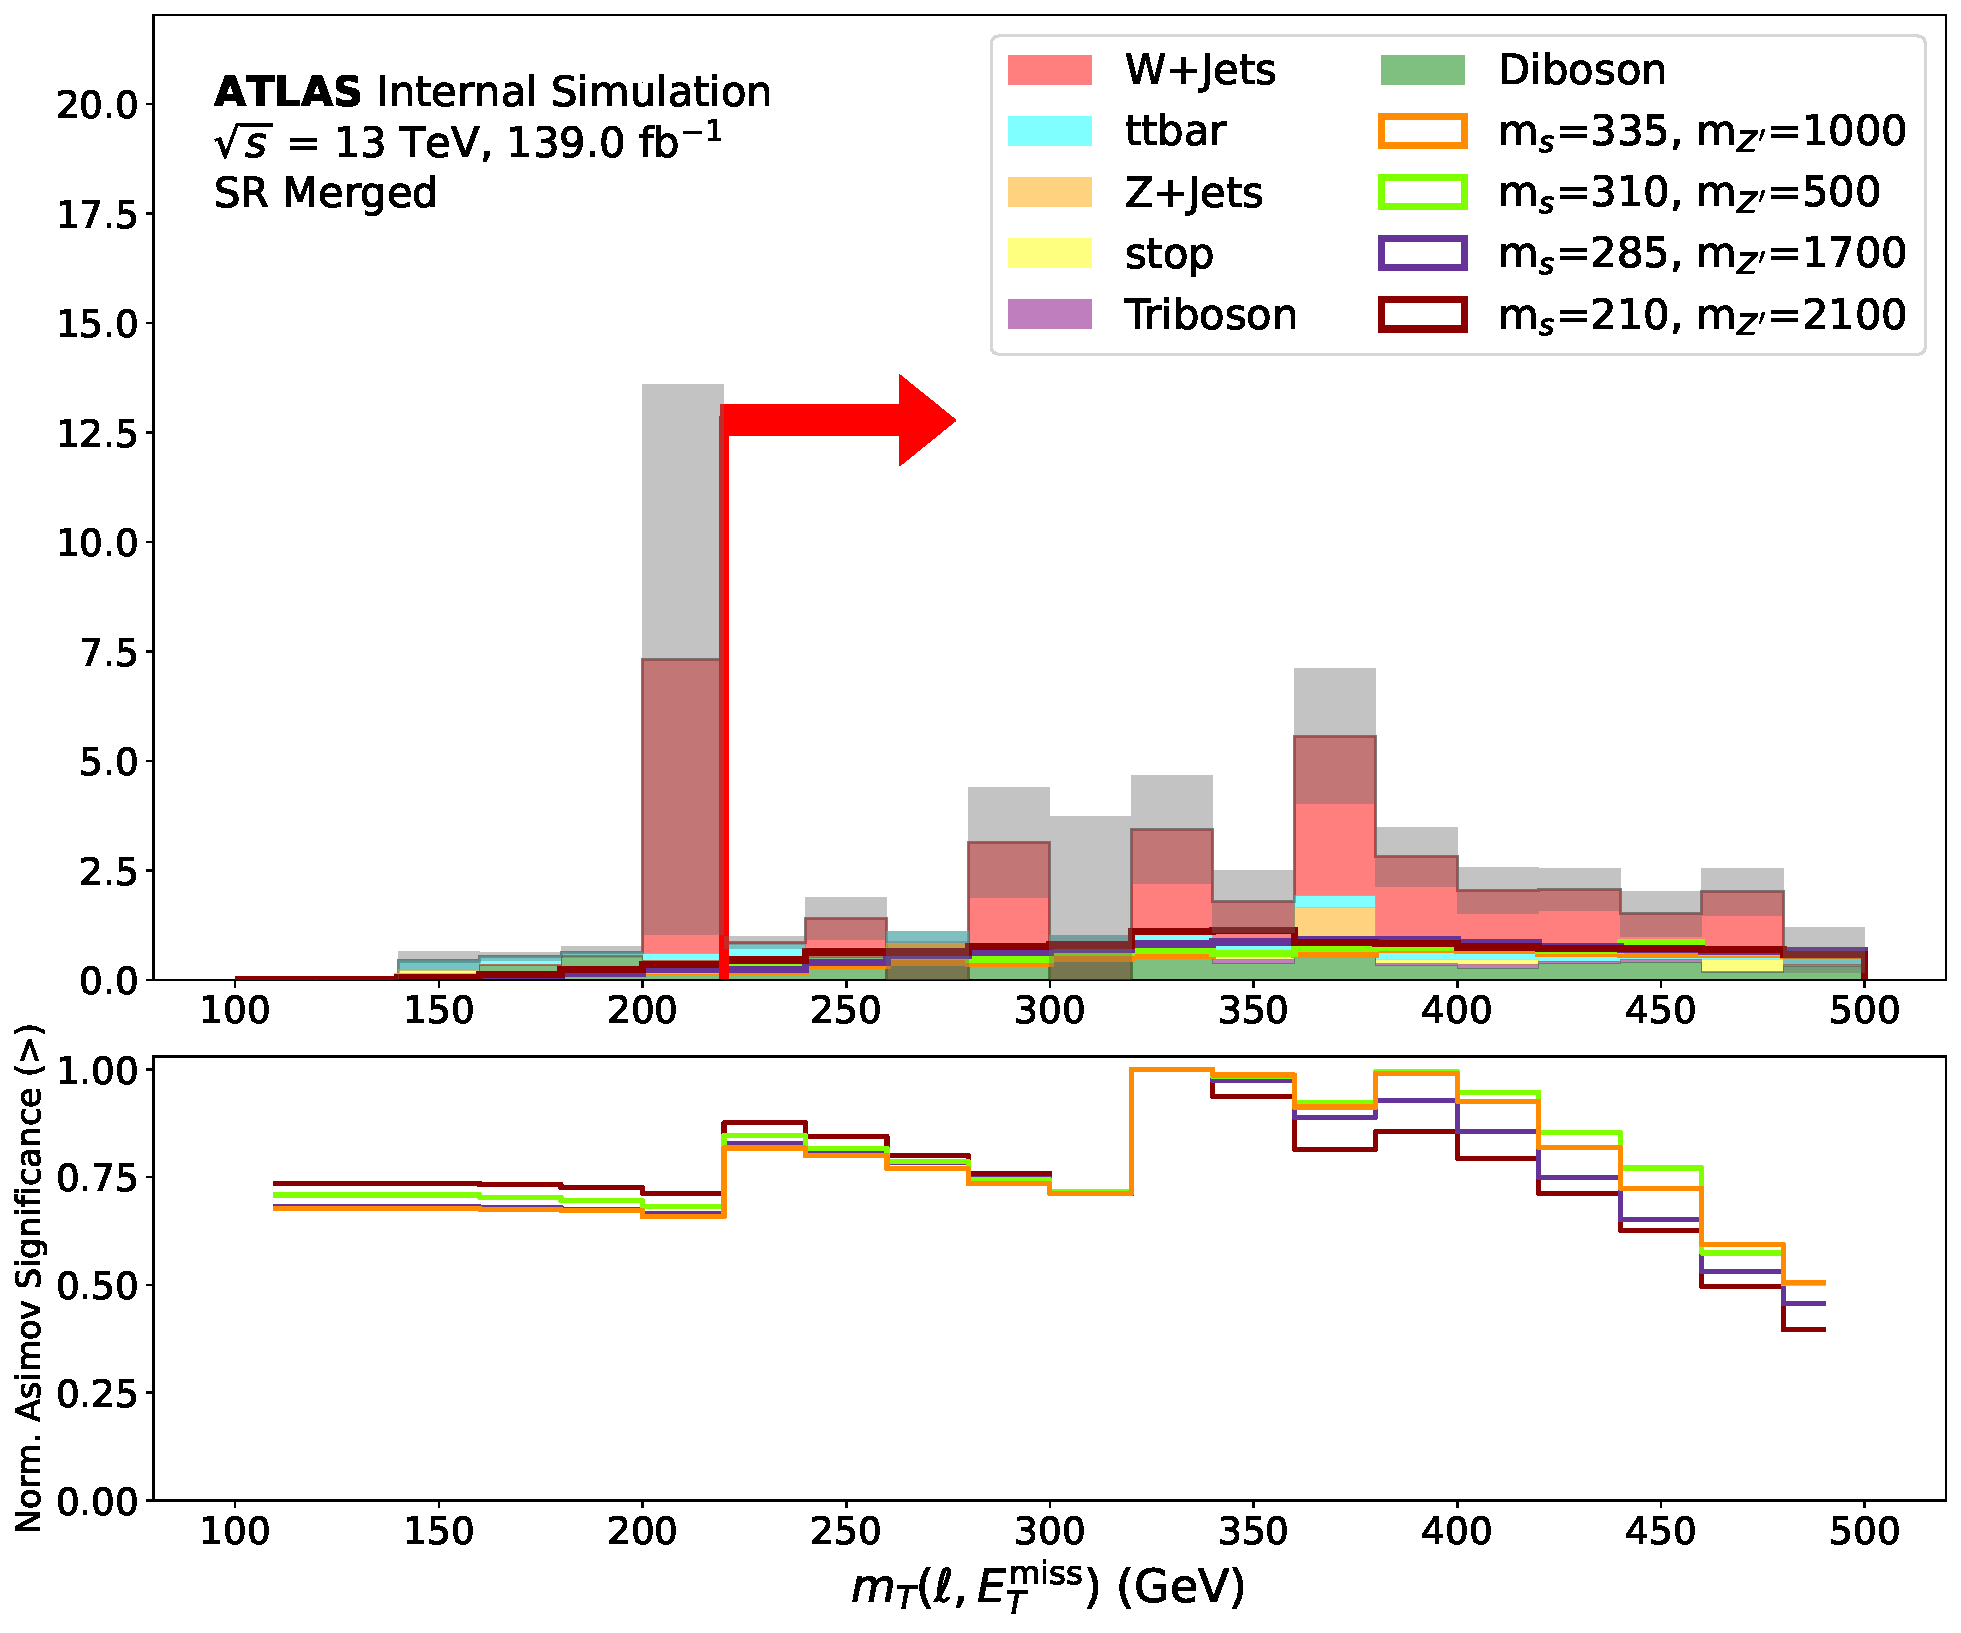
\includegraphics[width = 0.9\textwidth]{Figures/5/SR1L_Merged/mT_lep_met_normSig_N_1.pdf}
%    \caption{\mtlepmet}
%    \end{subfigure}
    \begin{subfigure}[t]{0.48\textwidth}
    \centering
     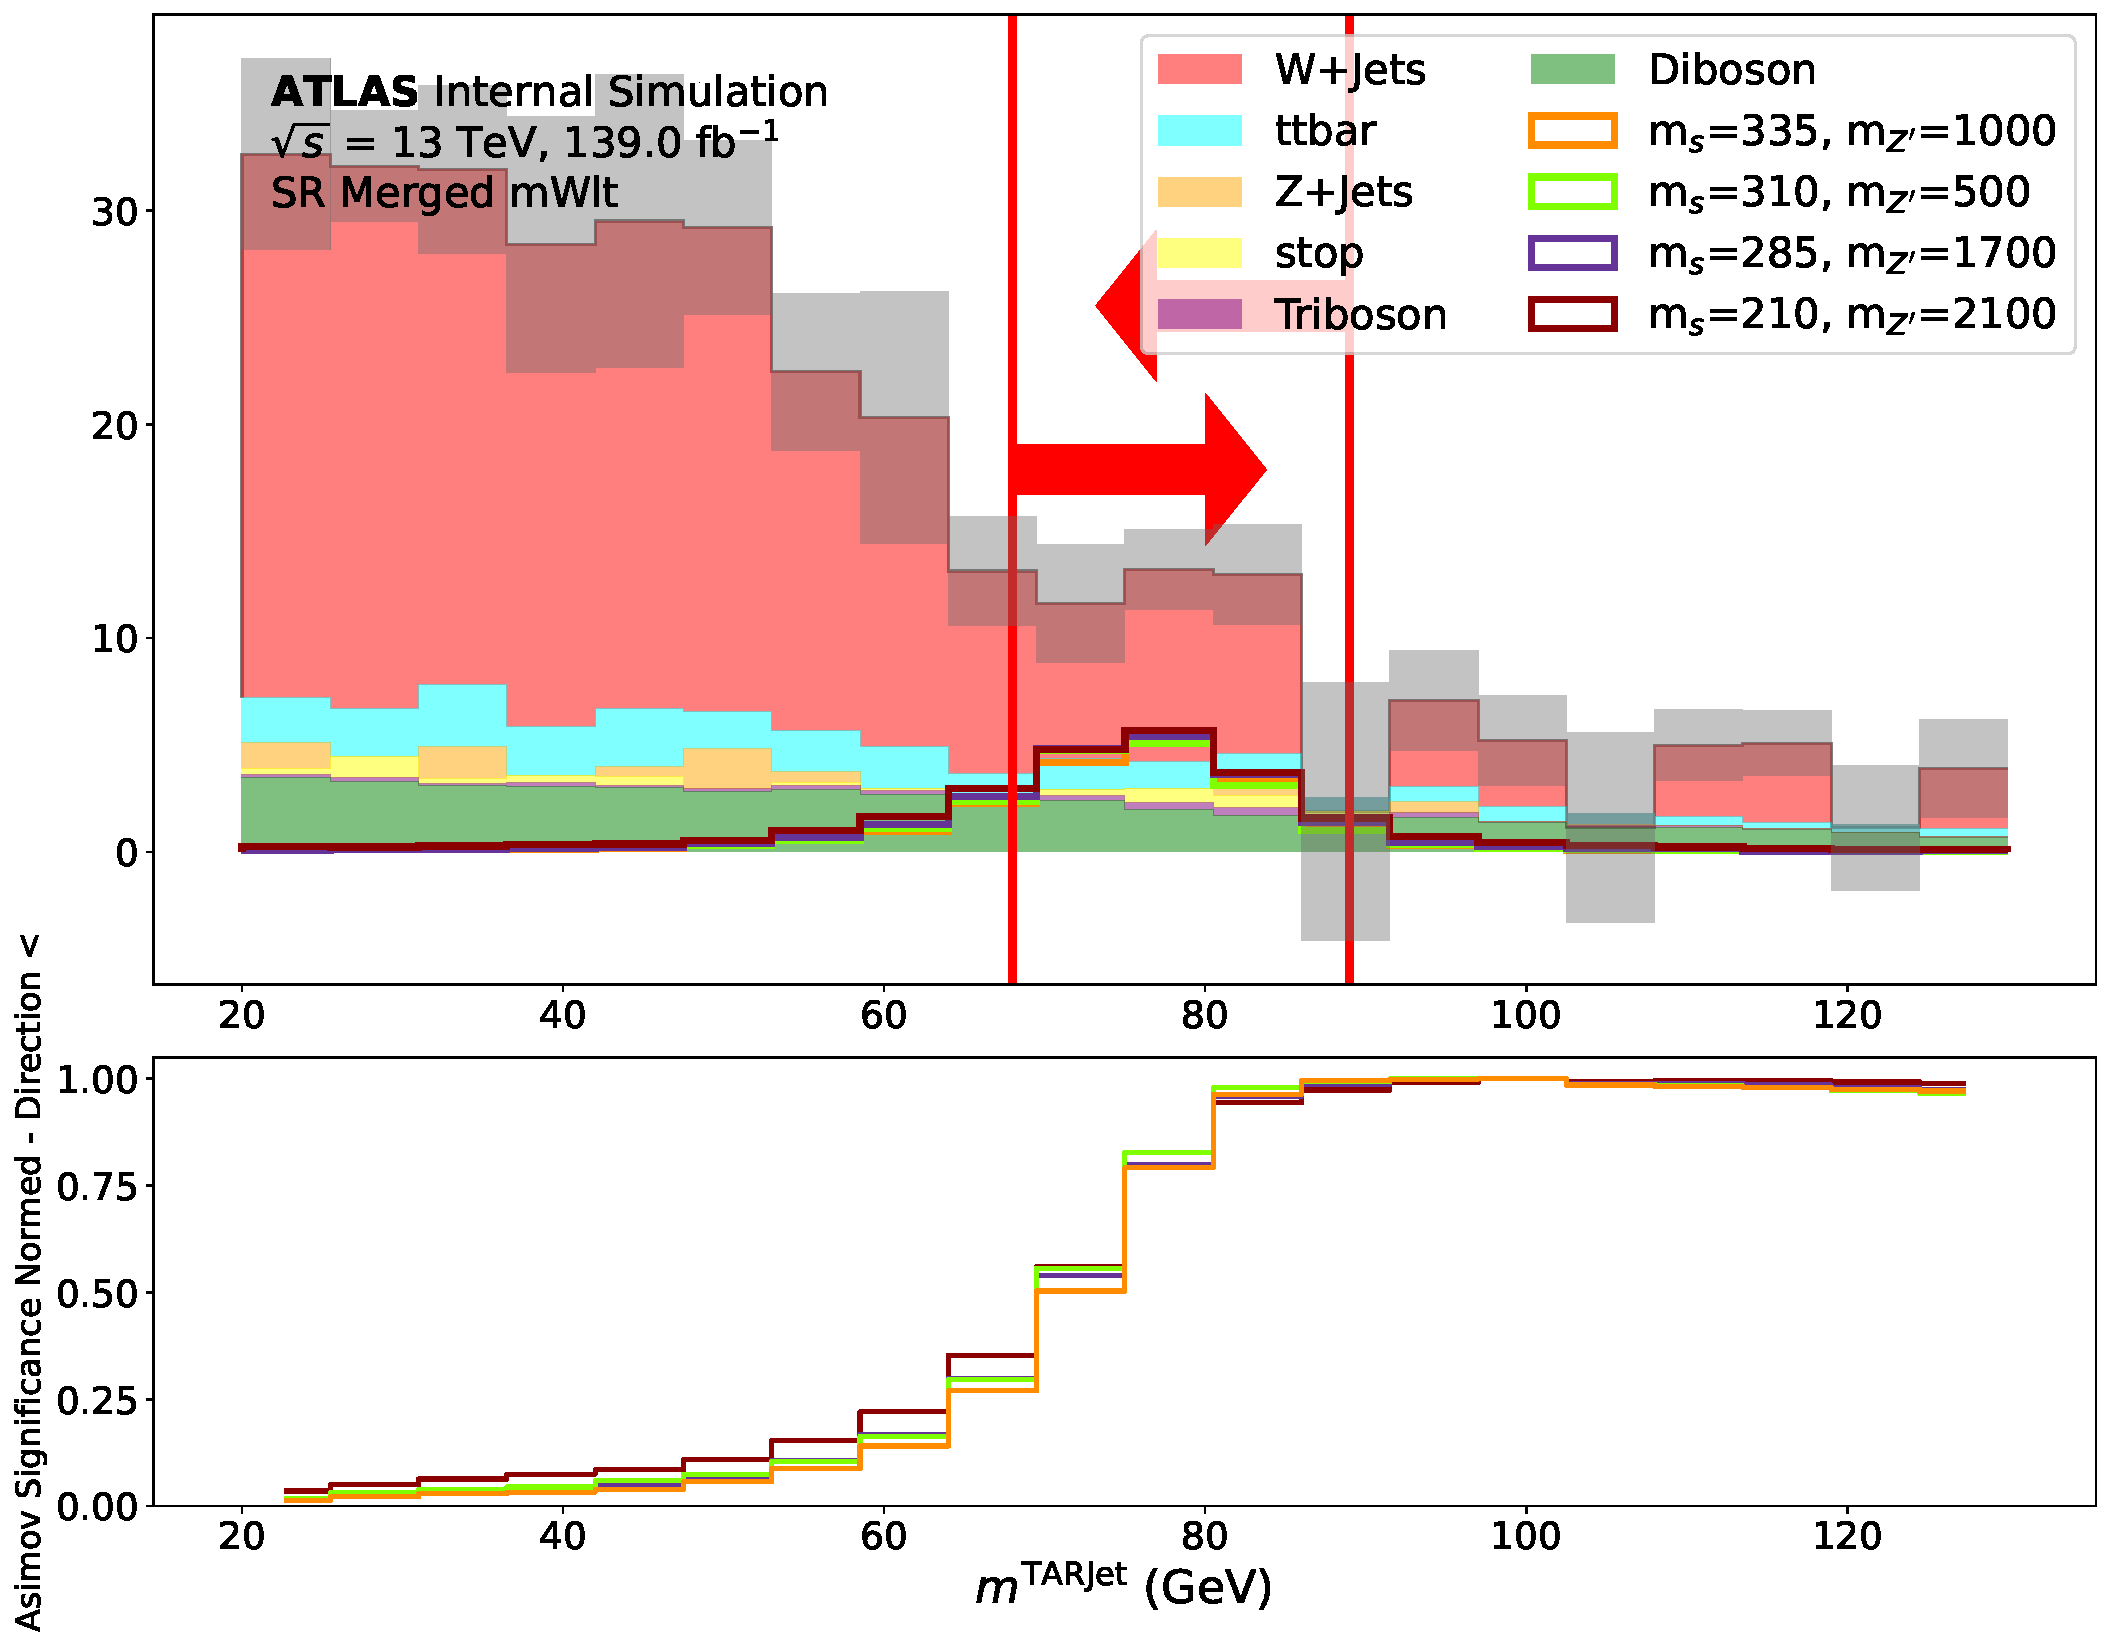
\includegraphics[width = 0.9\textwidth]{Figures/5/SR1L_Merged_mWlt/TARJets10_mTAR0_normSig_N_1.pdf}
     \caption{\mTAR Cut (\(Z\) evaluated for upper bound)}
    \end{subfigure}
    \begin{subfigure}[t]{0.48\textwidth}
    \centering
     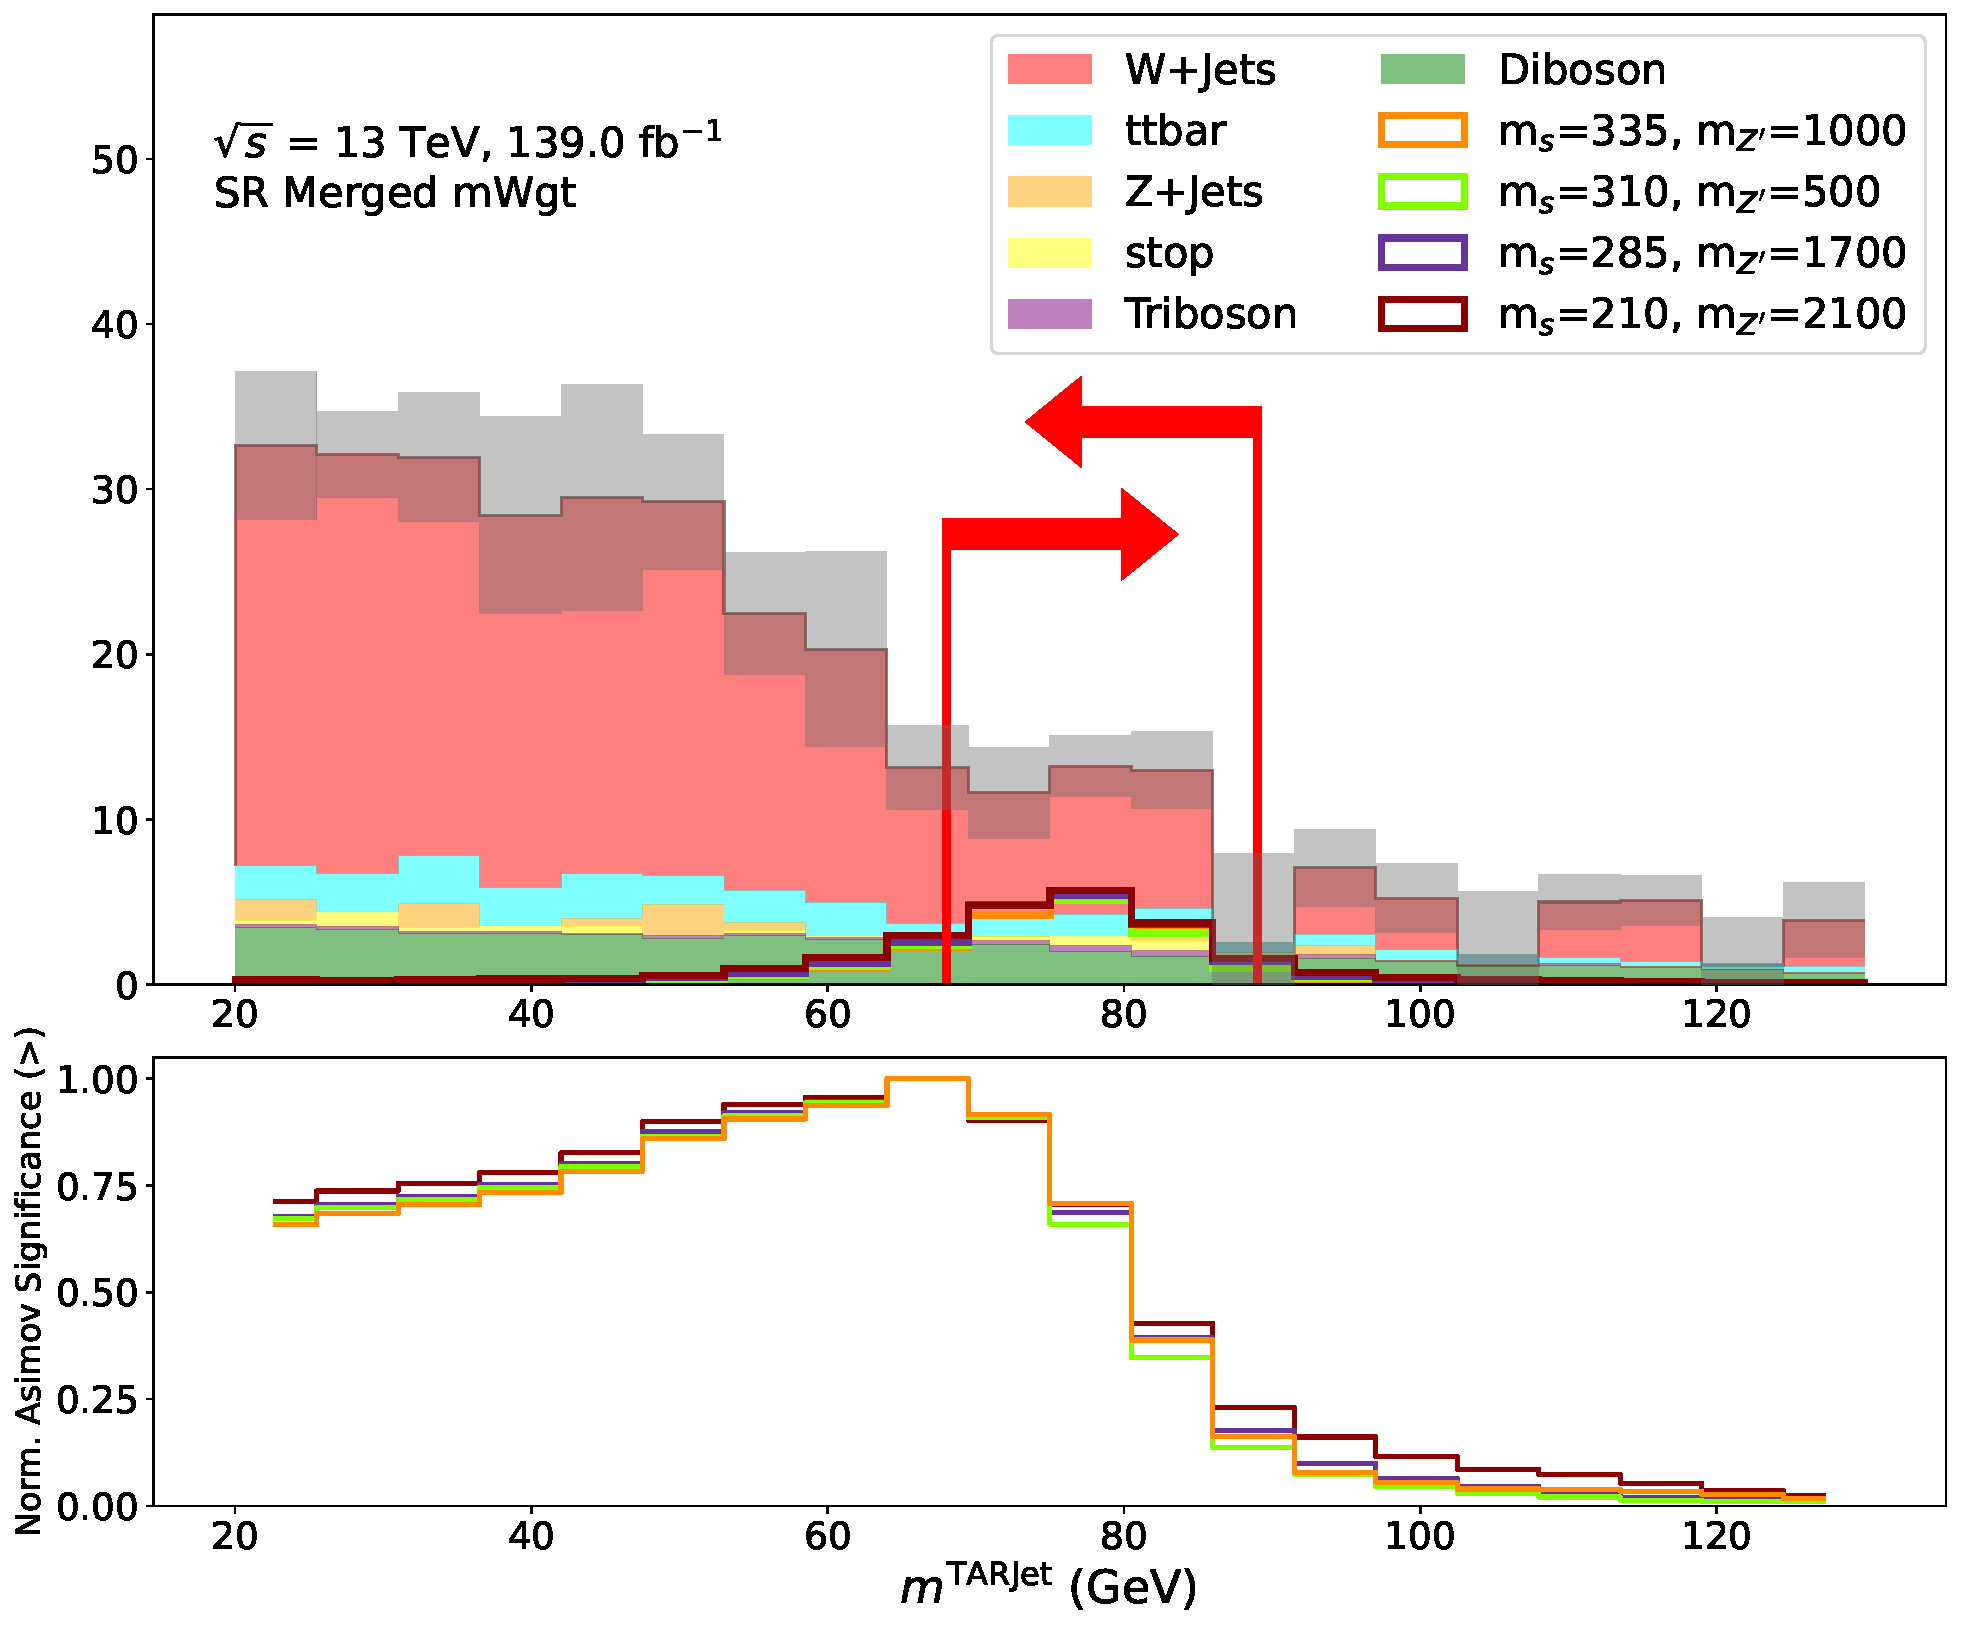
\includegraphics[width = 0.9\textwidth]{Figures/5/SR1L_Merged_mWgt/TARJets10_mTAR0_normSig_N_1.pdf}
     \caption{\mTAR Cut  (\(Z\) evaluated for lower bound)}
    \end{subfigure}
        \begin{subfigure}[t]{0.48\textwidth}
    \centering
     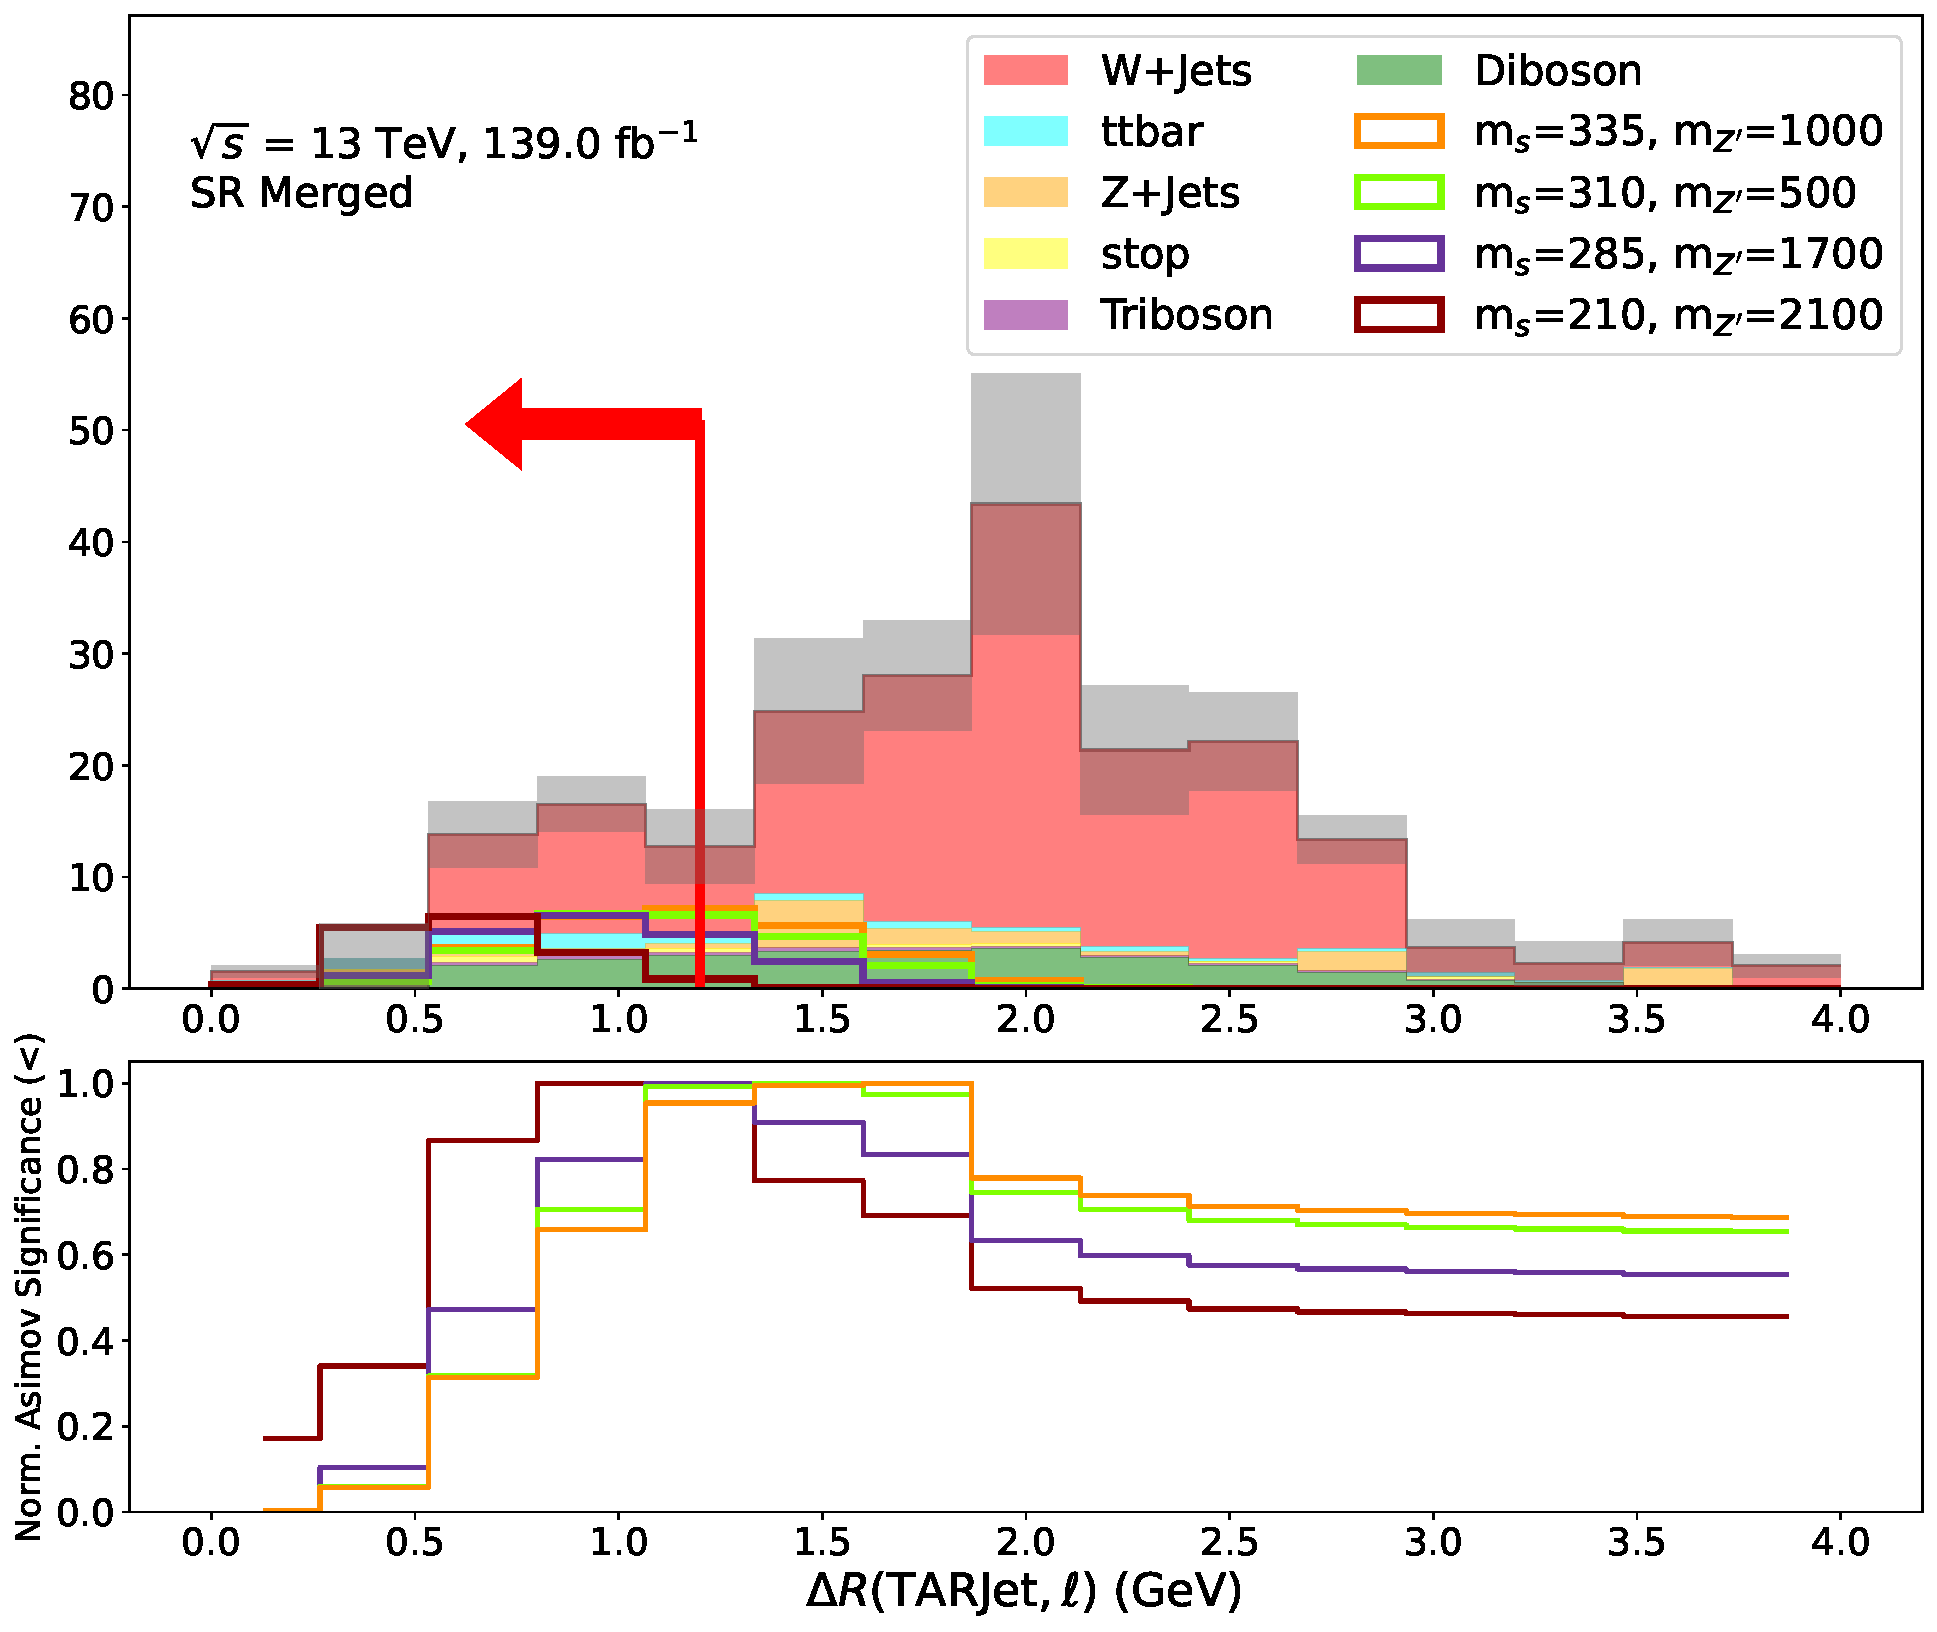
\includegraphics[width = 0.9\textwidth]{Figures/5/SR1L_Merged/dR_lep_TARJets10_normSig_N_1.pdf}
    \caption{\drTARl}
    \end{subfigure}
%    \begin{subfigure}[t]{0.48\textwidth}
%    \centering
%     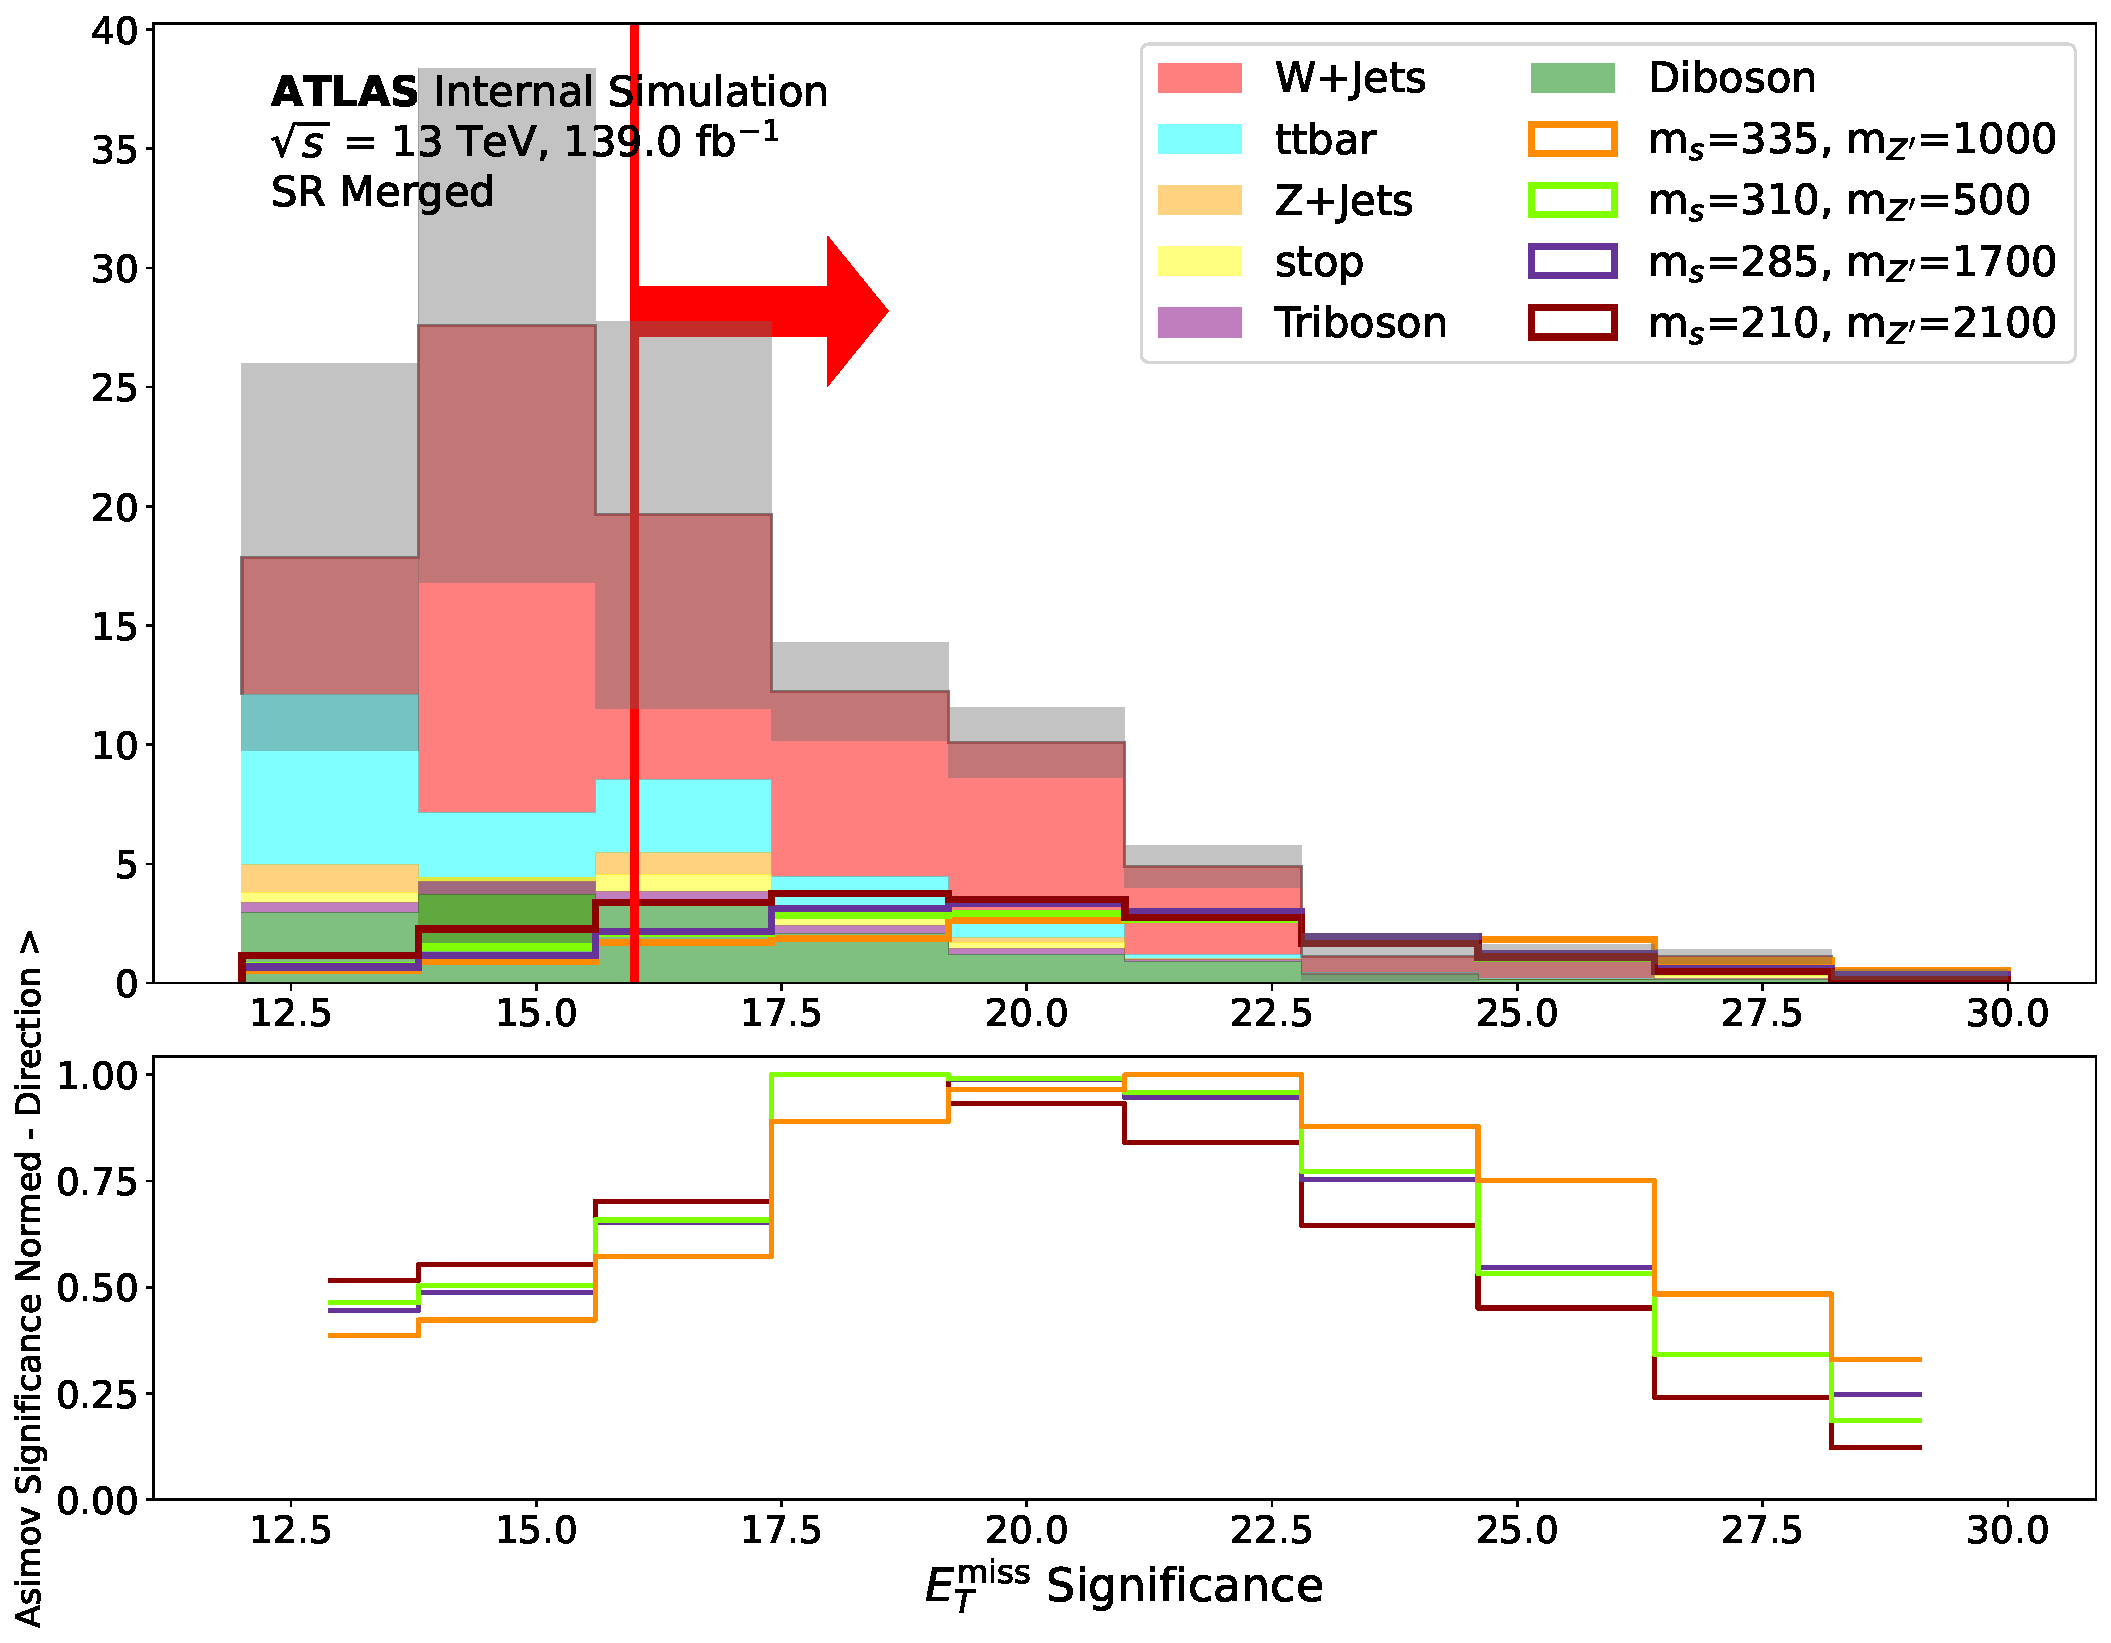
\includegraphics[width = 0.9\textwidth]{Figures/5/SR1L_Merged/MetTST_Significance_normSig_N_1.pdf}
%    \caption{\metsig}
%    \end{subfigure}
%    \begin{subfigure}[t]{0.48\textwidth}
%    \centering
%     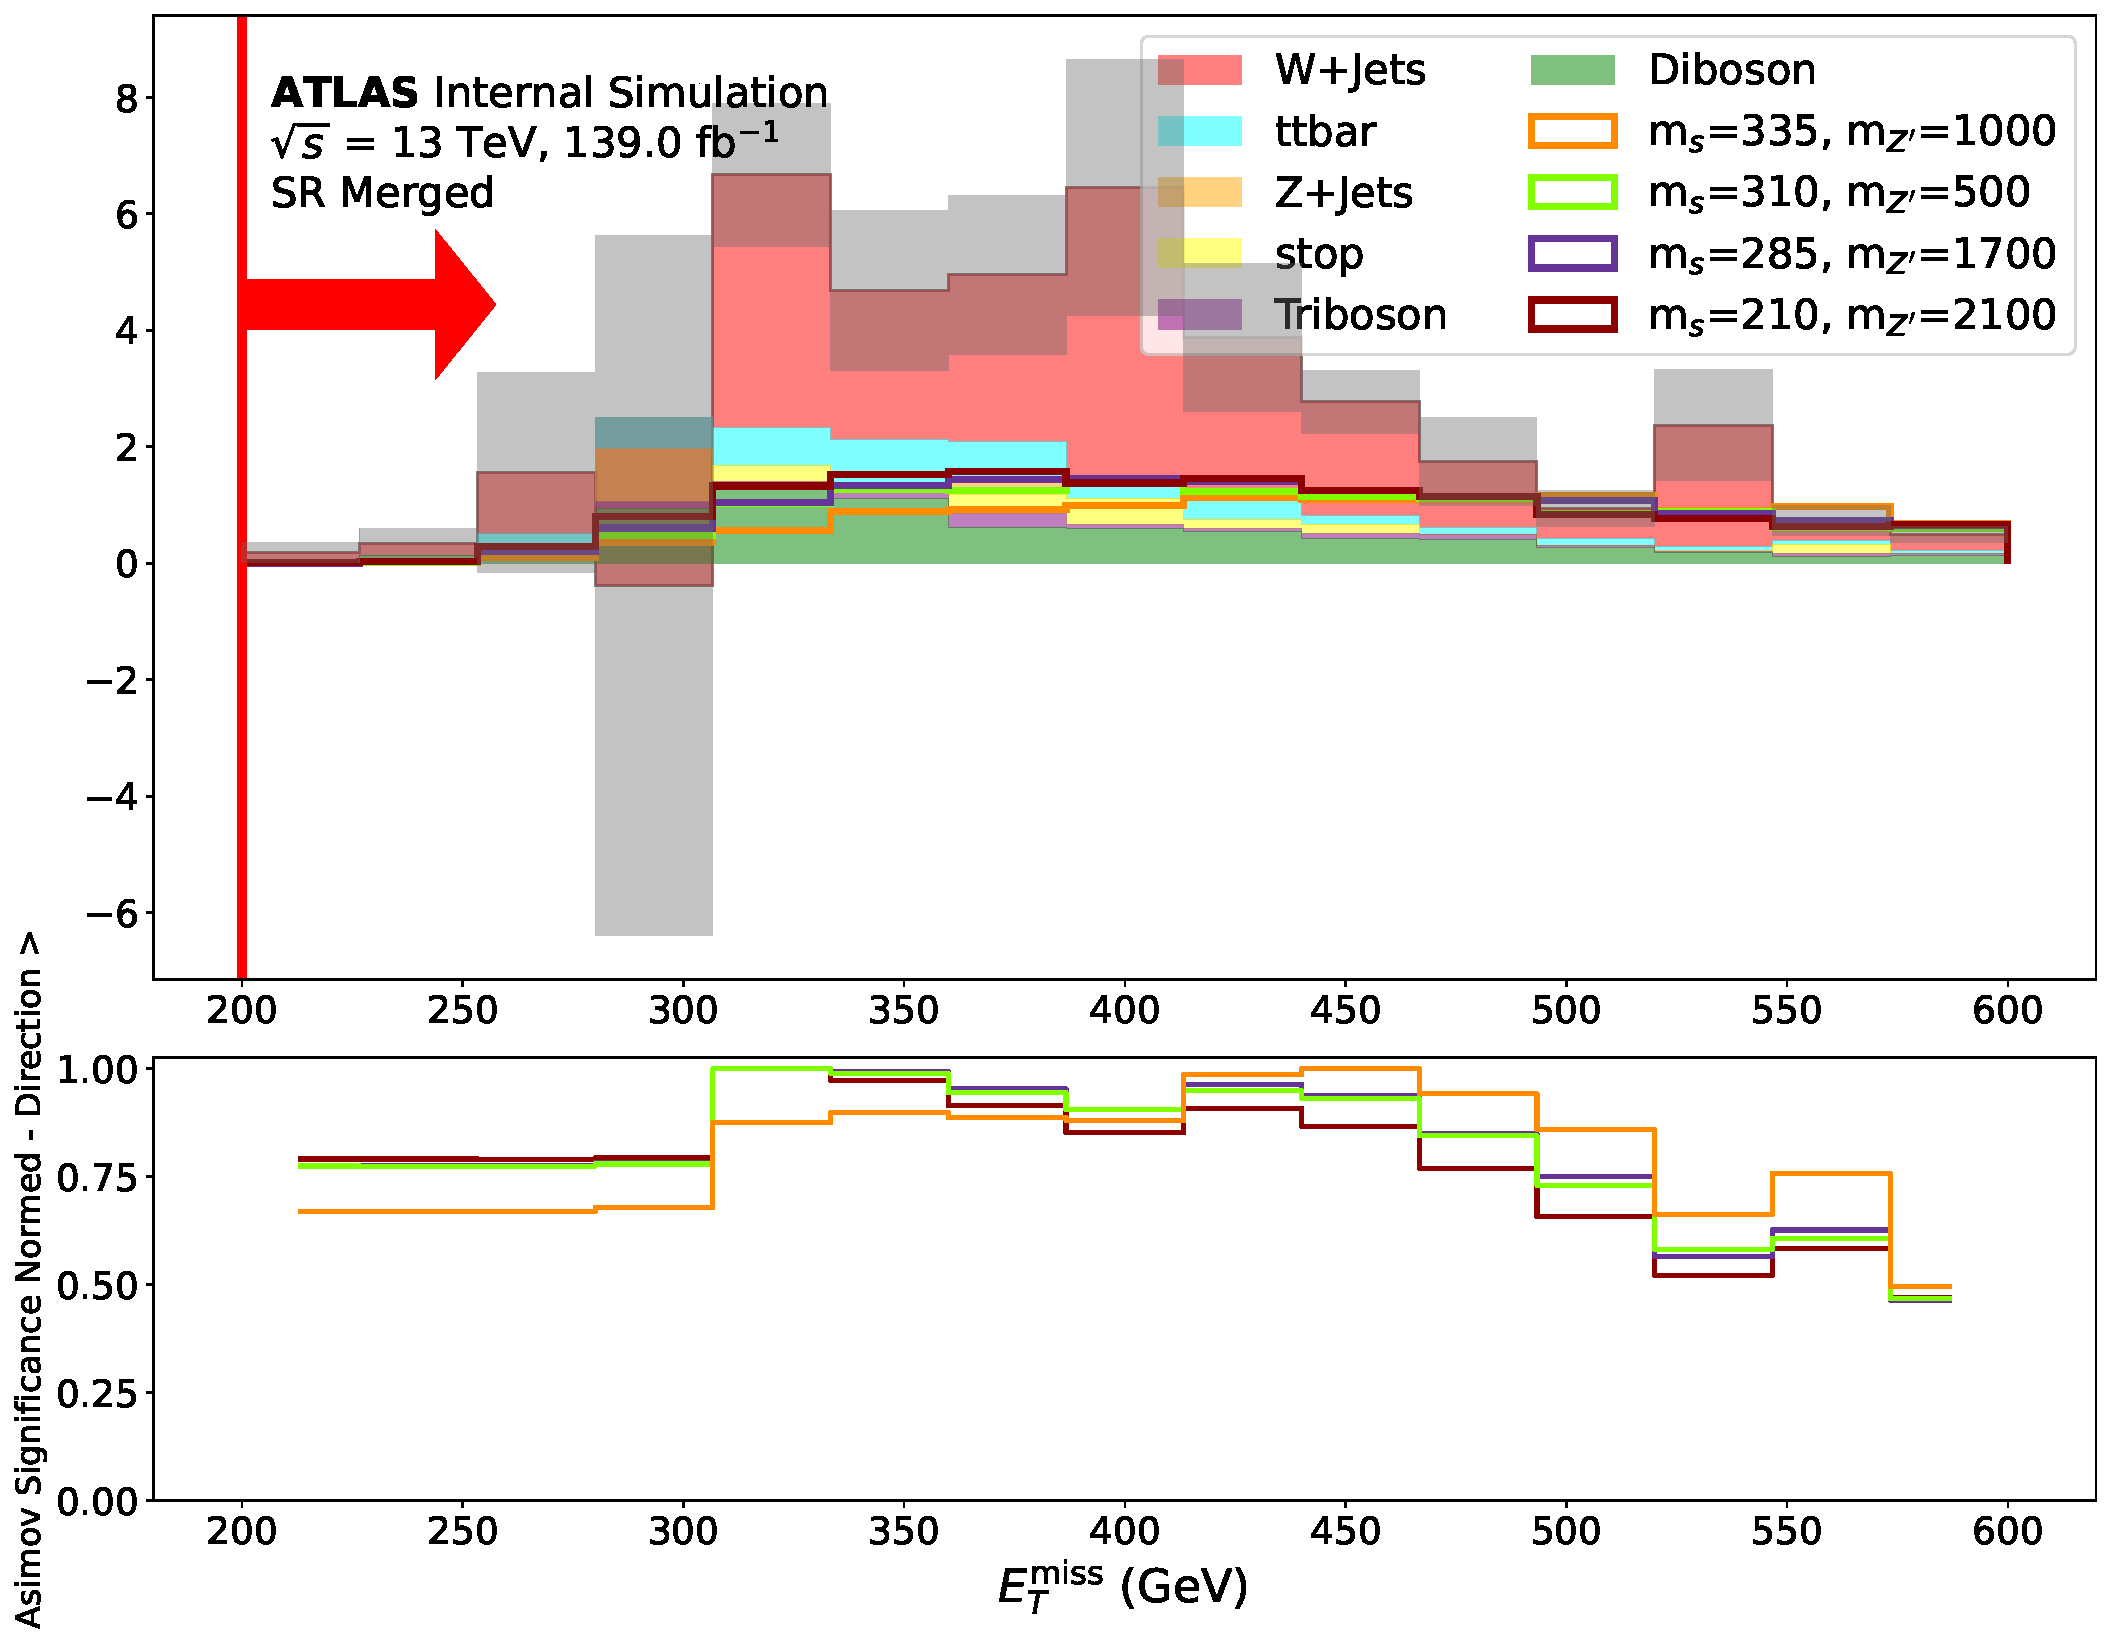
\includegraphics[width = 0.9\textwidth]{Figures/5/SR1L_Merged/MetTST_met_normSig_N_1.pdf}
%    \caption{\met}
%    \end{subfigure}
   \caption[N-1 Distributions for the \mTAR and \drTARl variables used in the merged signal region definition.]{N-1 Distributions for the \mTAR and \drTARl variables used in the merged signal region definition. Grey bands show statistical uncertainty on background estimate. The lower panel shows the cumulative Asimov significance normalized to unit peak, where the direction (\(>\) or \(<\)) specified in the y label indicates whether the significance is being summed from above (\(>\)) or from below (\(<\)). Red vertical line and arrow show placement and direction of selection on the given variable in this region.}
   \label{fig:Nminus1mergedSR}
\end{figure}
% \begin{figure} \ContinuedFloat
%    \begin{subfigure}[t]{0.48\textwidth}
%    \centering
%     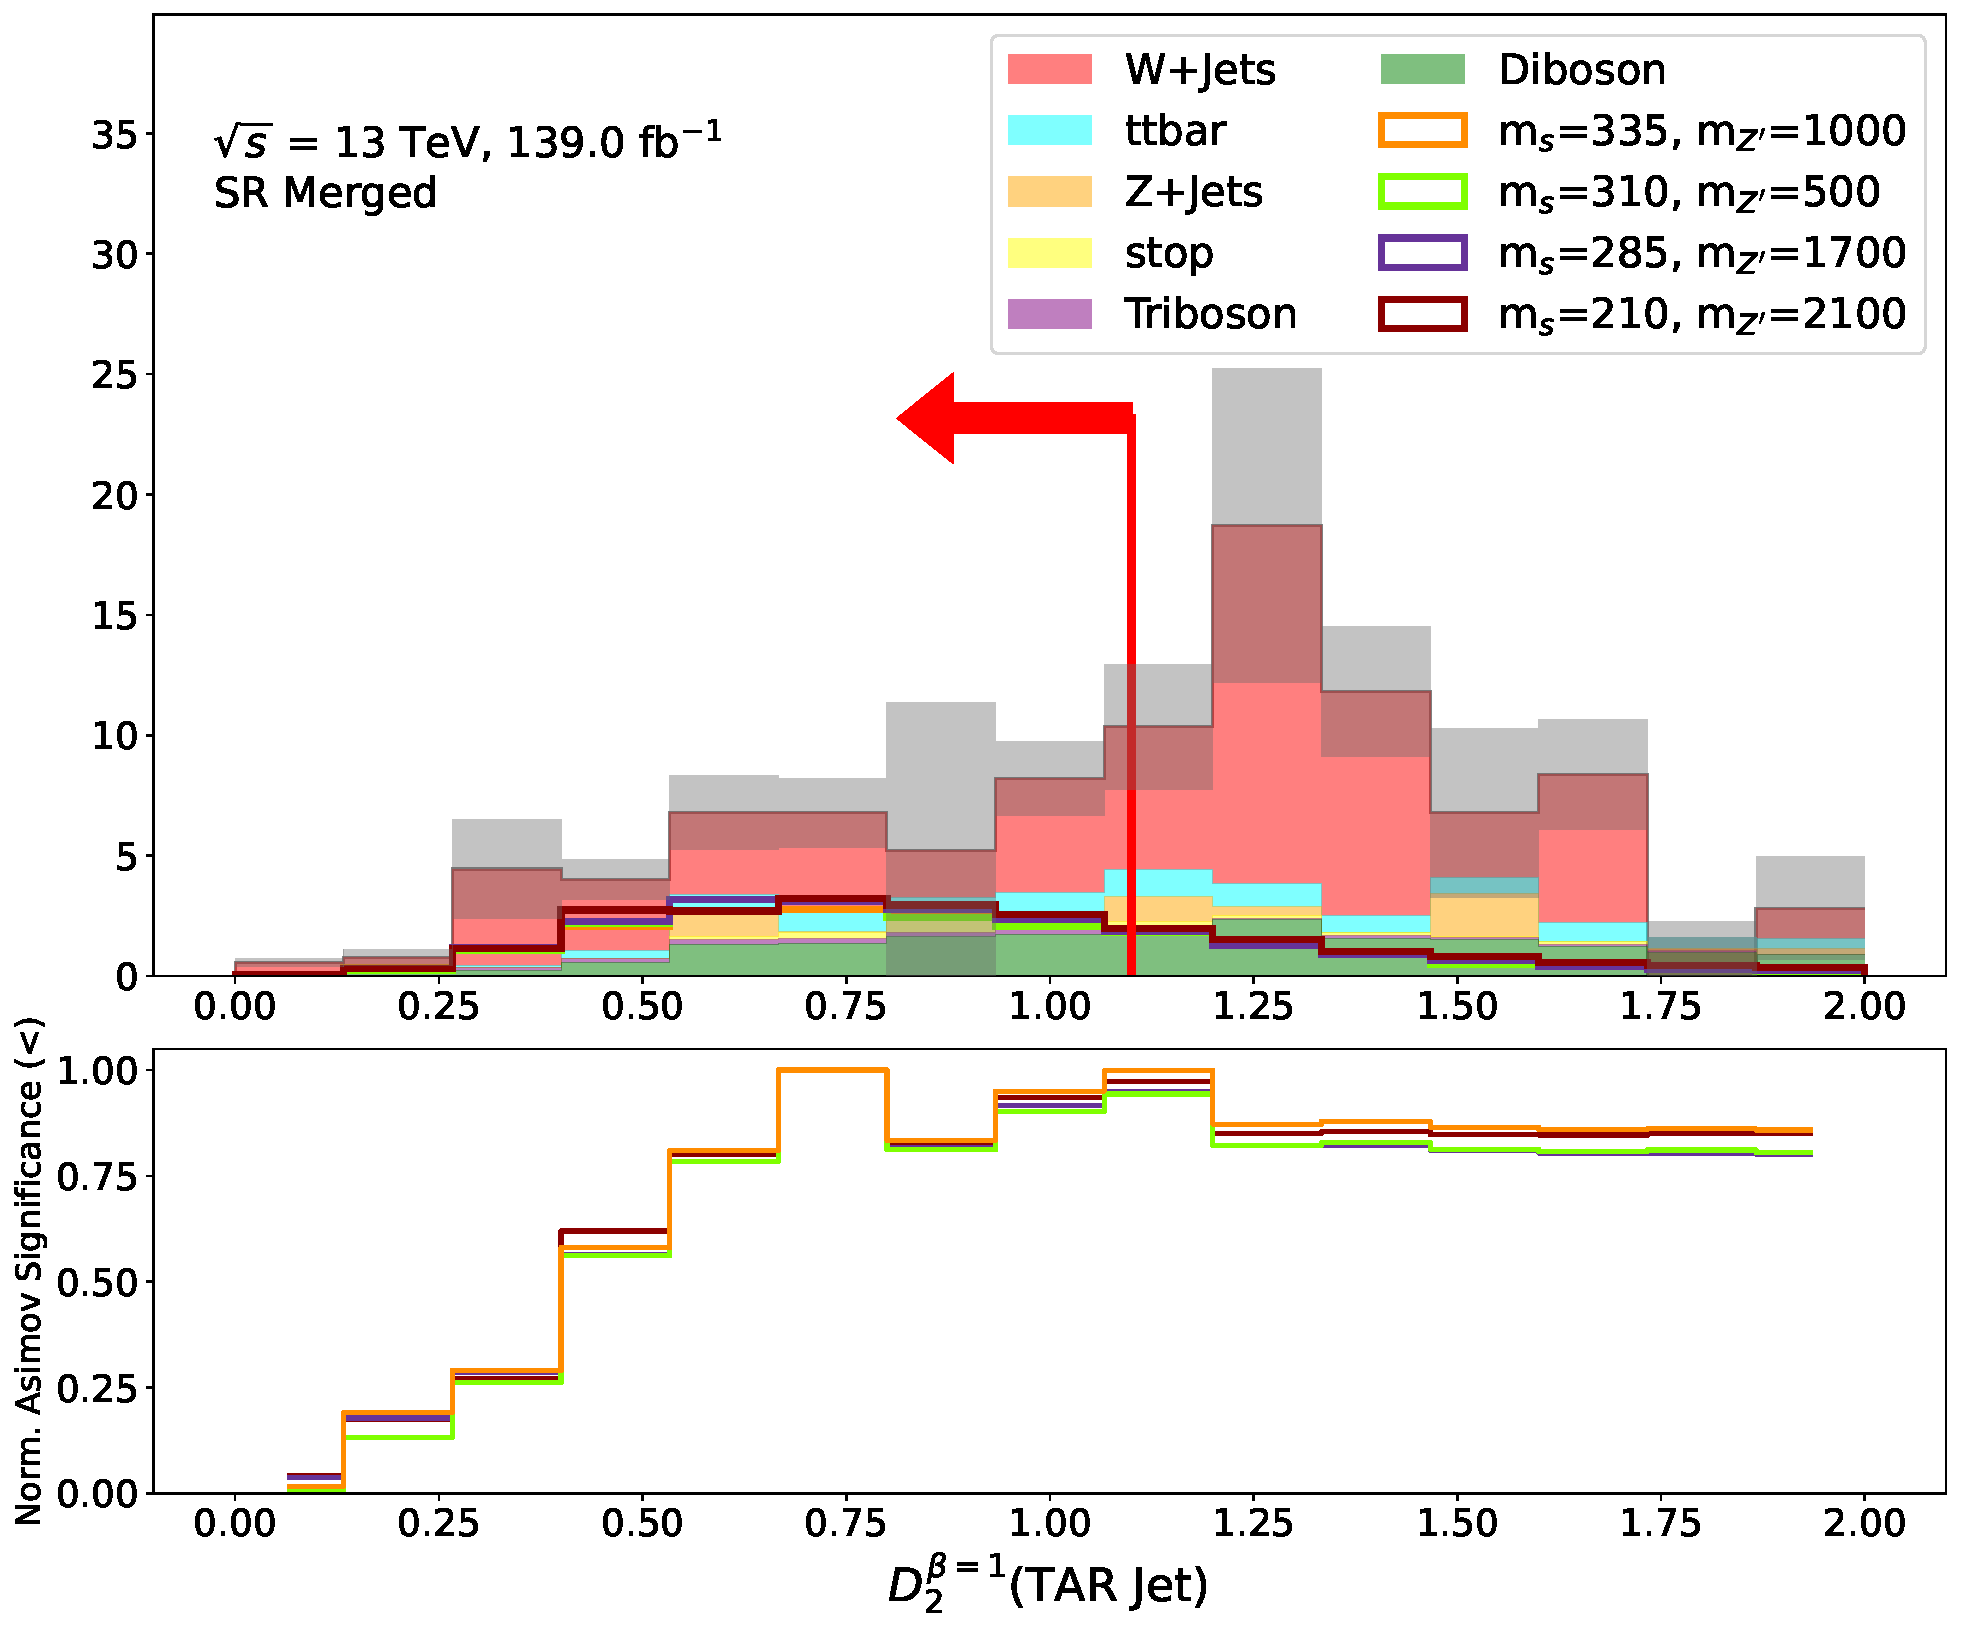
\includegraphics[width = 0.9\textwidth]{Figures/5/SR1L_Merged/TARJets10_TAR_D20_normSig_N_1.pdf}
%    \caption{\DtwoTAR}
%    \end{subfigure}
%    \caption{N-1 Distributions for selection requirements in the merged signal region (continued)}
%  \end{figure}
  
  \begin{figure}[htbp]
  \centering
%    \begin{subfigure}[t]{0.48\textwidth}
%    \centering
%     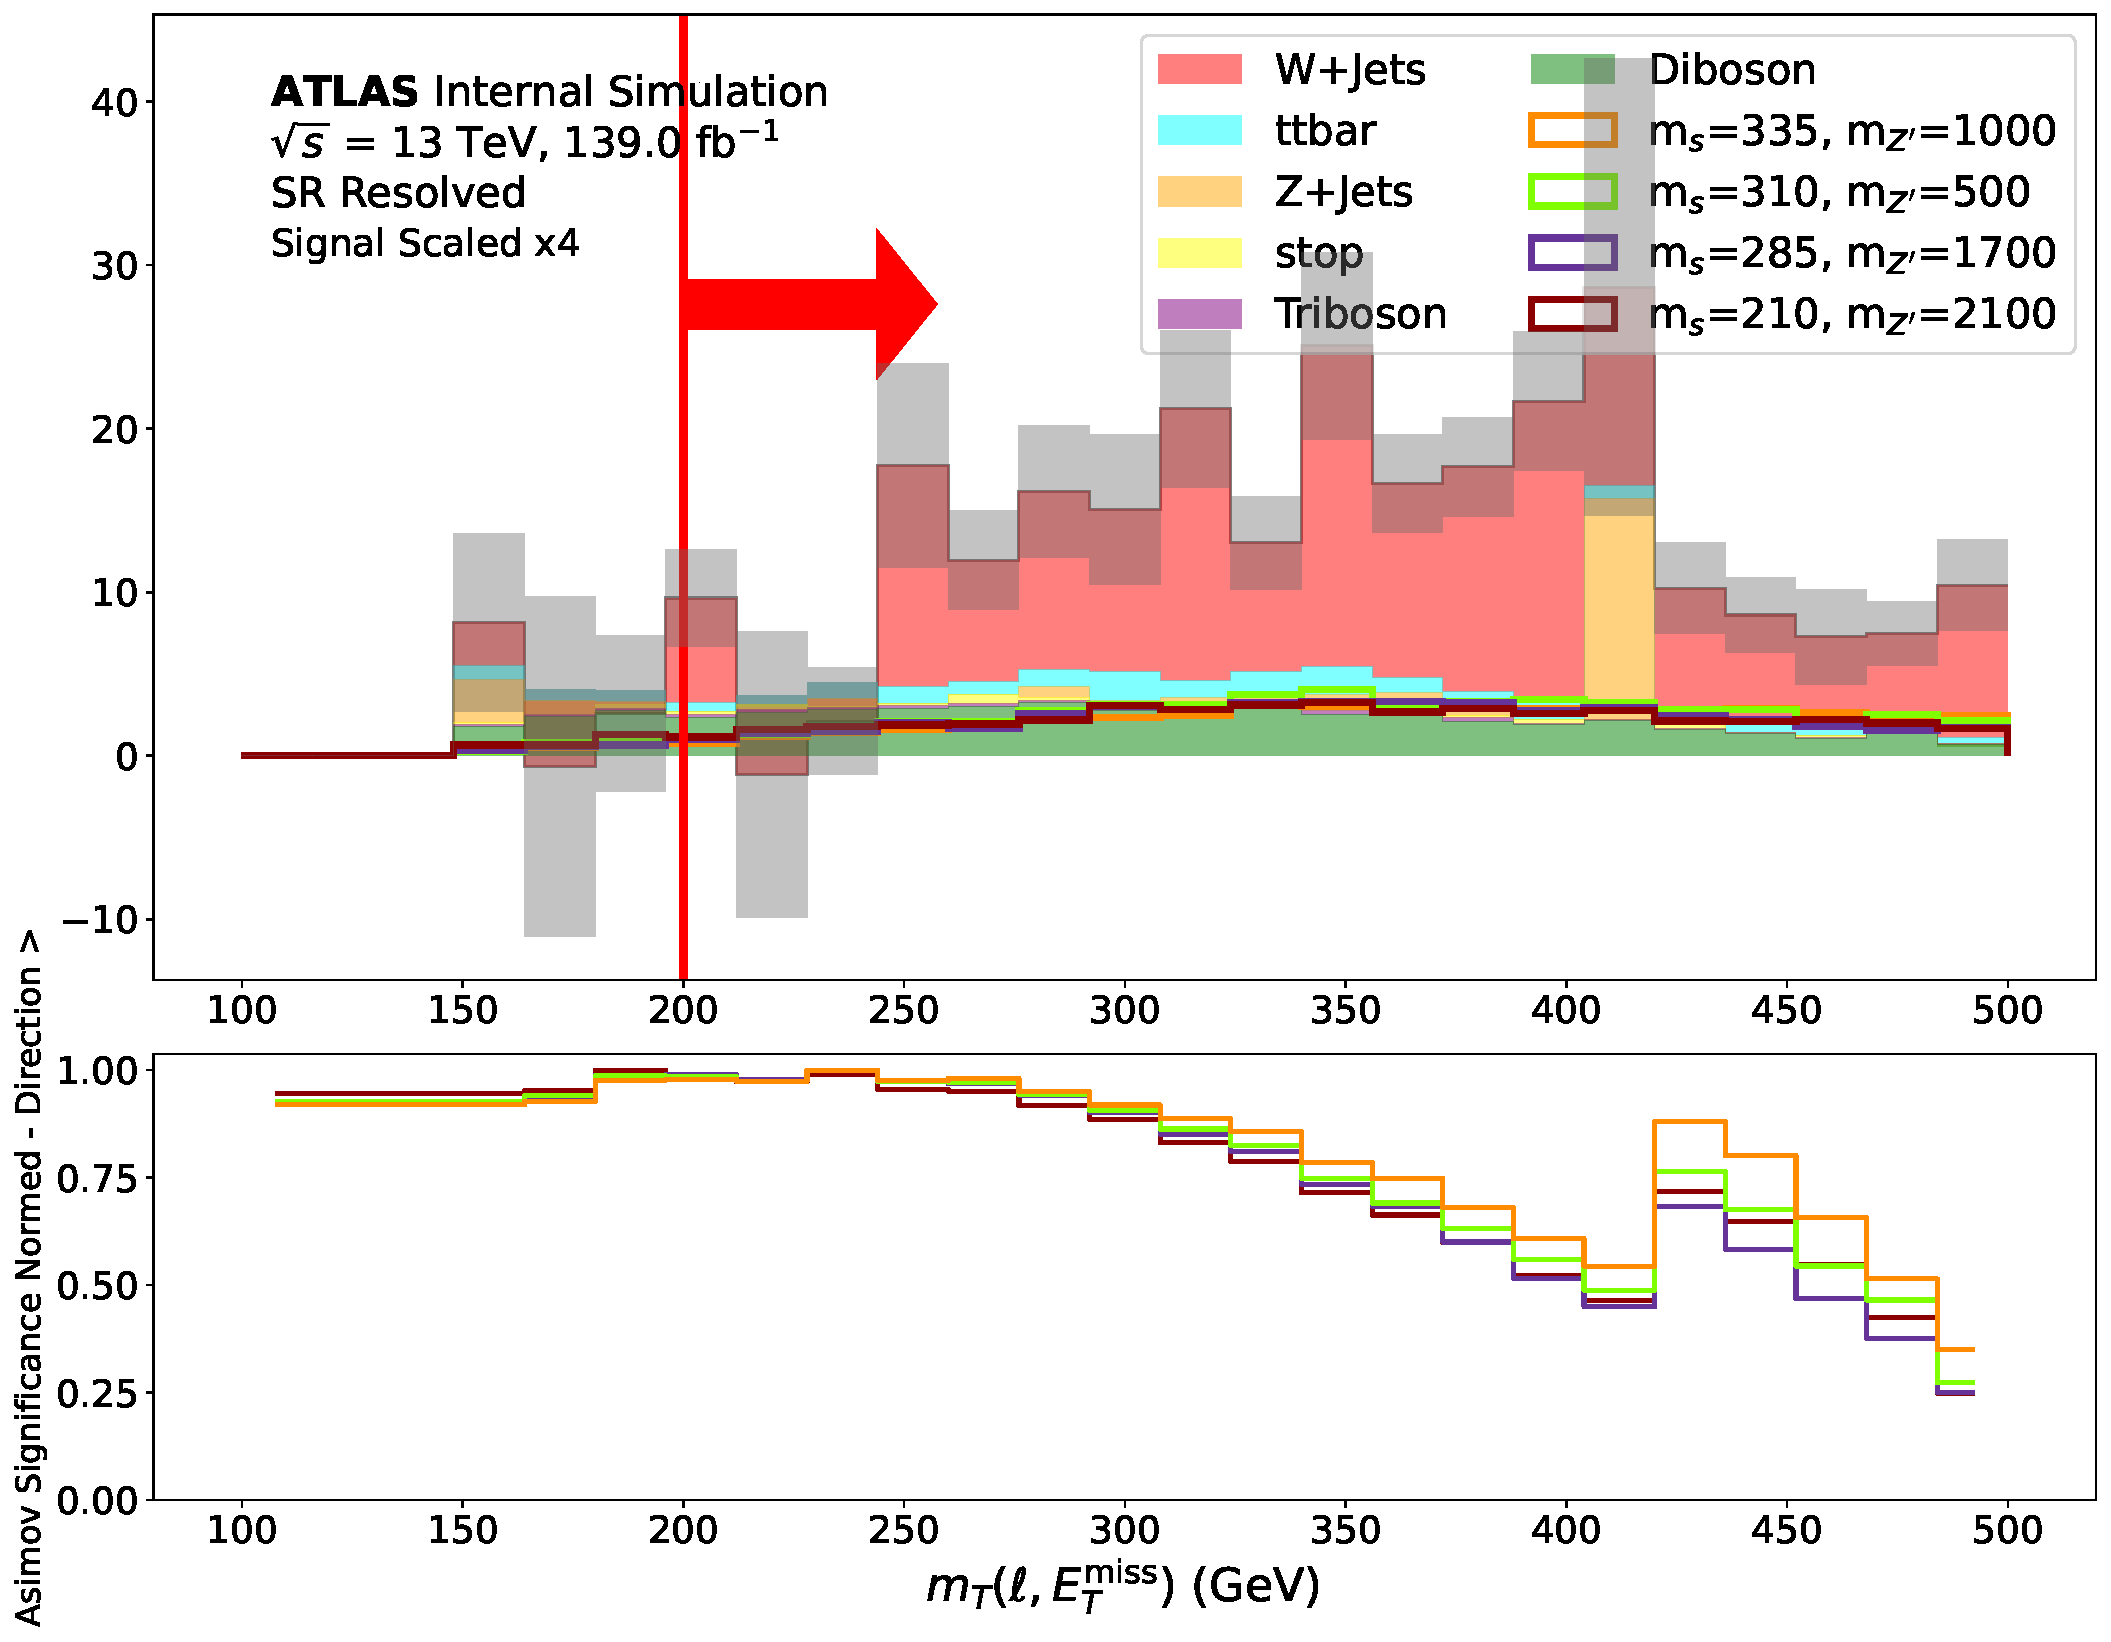
\includegraphics[width = 0.9\textwidth]{Figures/5/SR1L_Resolved/mT_lep_met_normSig_N_1.pdf}
%    \caption{\mtlepmet}
%    \end{subfigure}
    \begin{subfigure}[t]{0.48\textwidth}
    \centering
     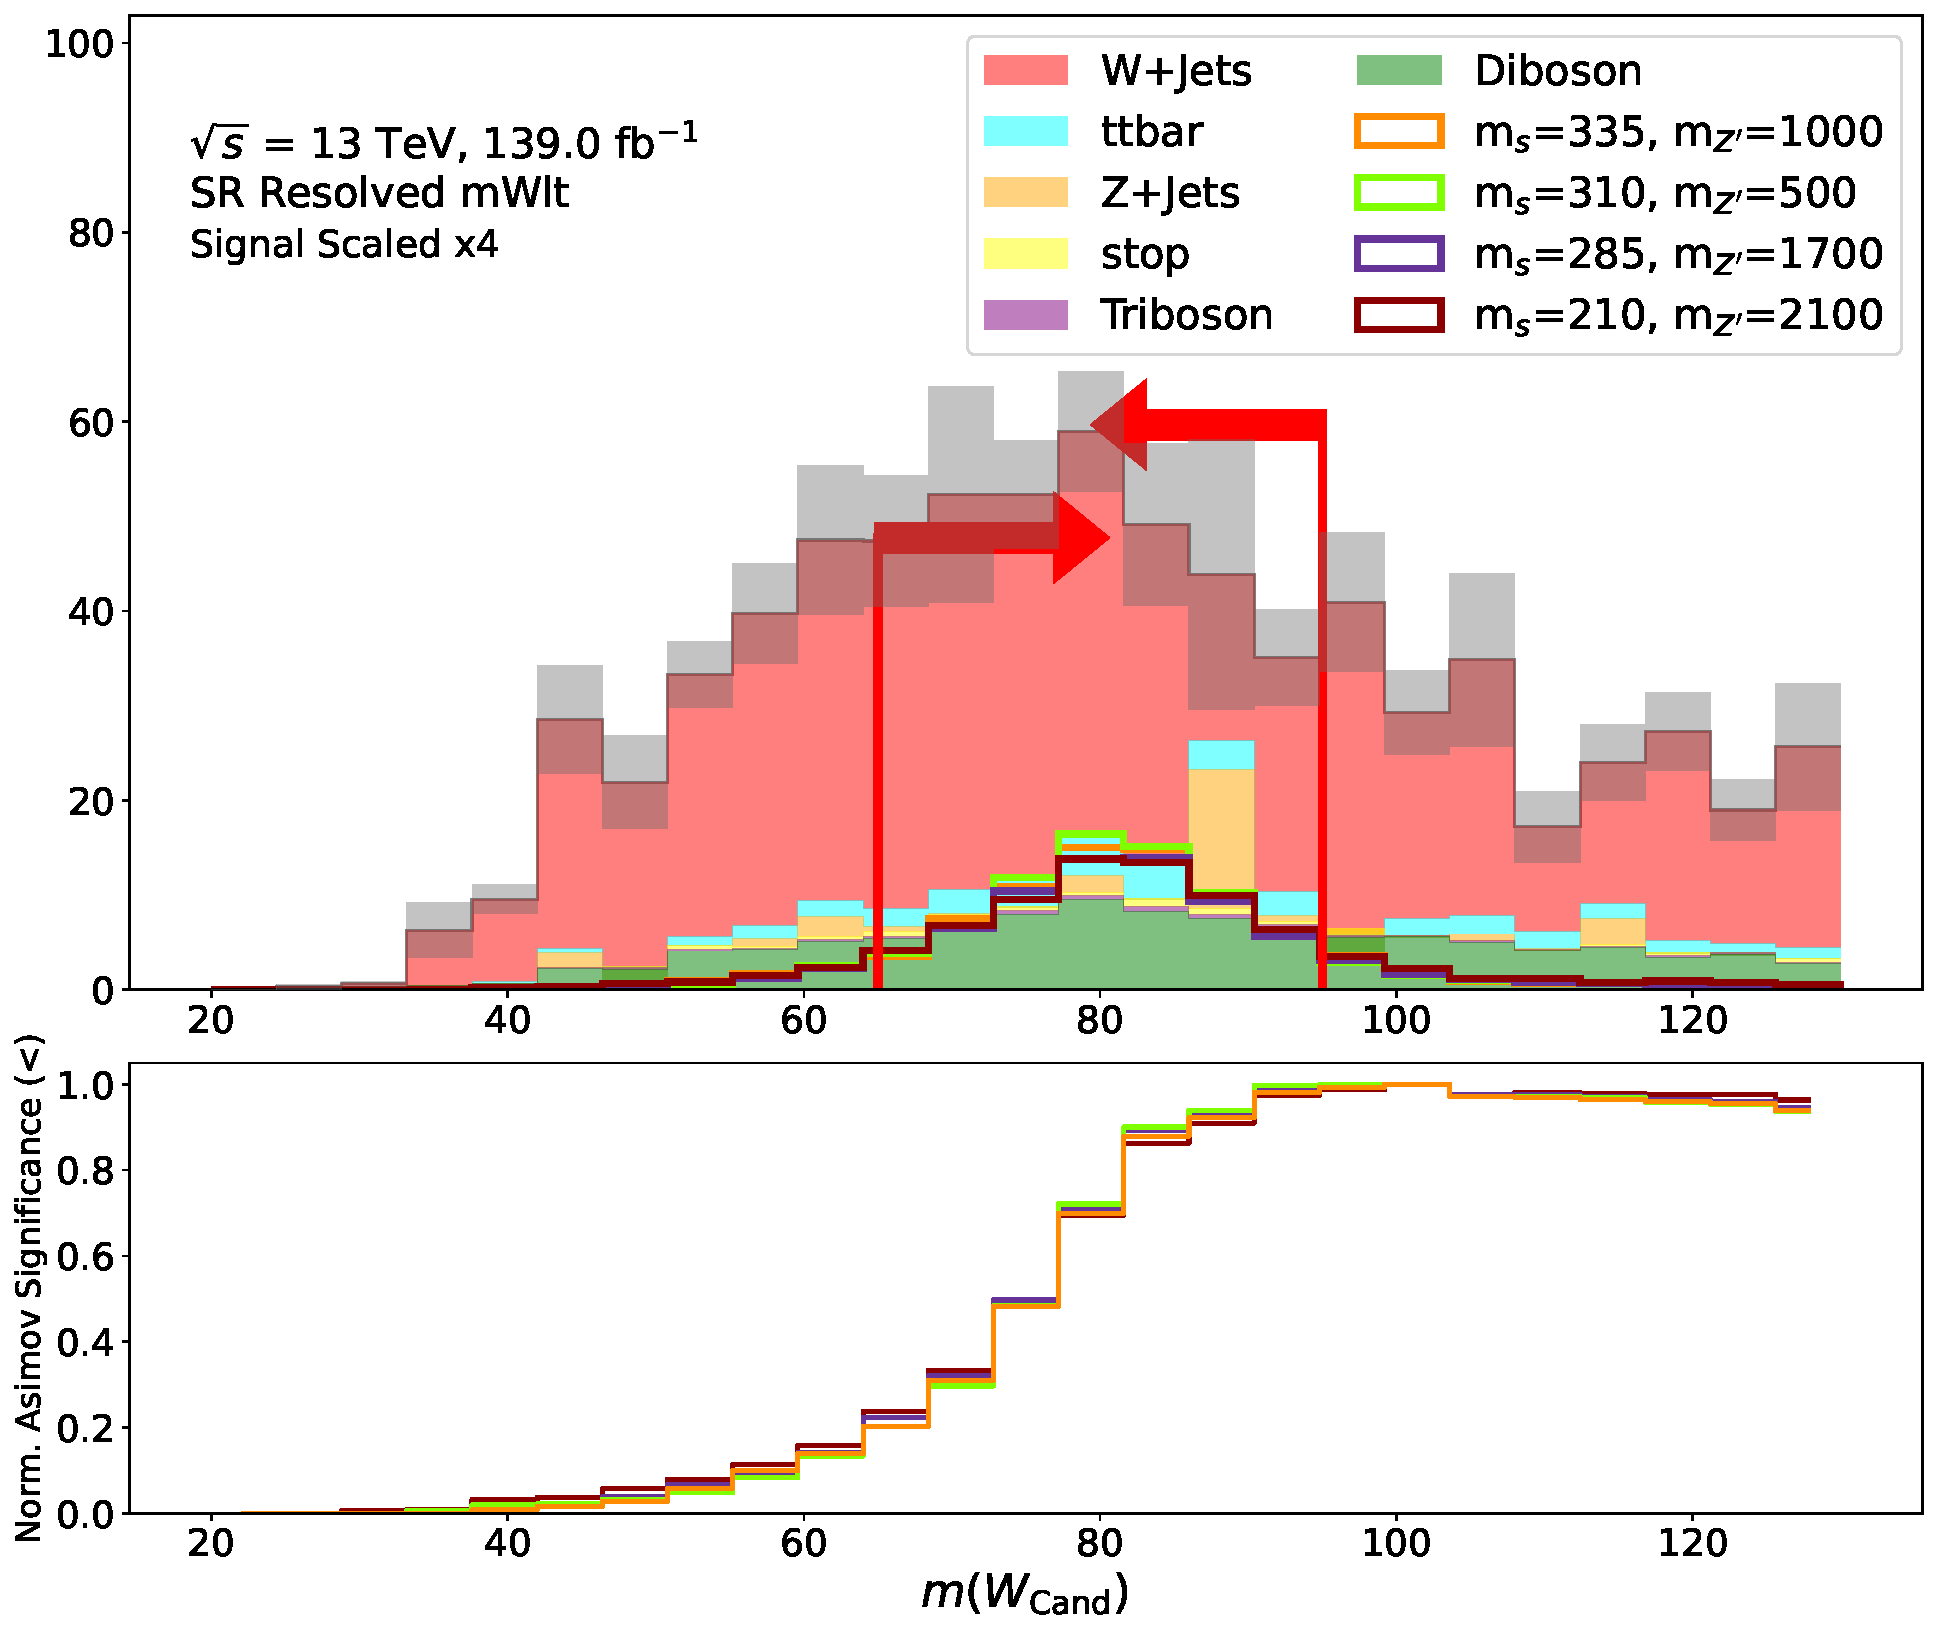
\includegraphics[width = 0.9\textwidth]{Figures/5/SR1L_Resolved_mWlt/WCand_m_normSig_N_1.pdf}
     \caption{\Wcandm Cut (\(Z\) evaluated for upper bound)}
    \end{subfigure}
    \begin{subfigure}[t]{0.48\textwidth}
    \centering
     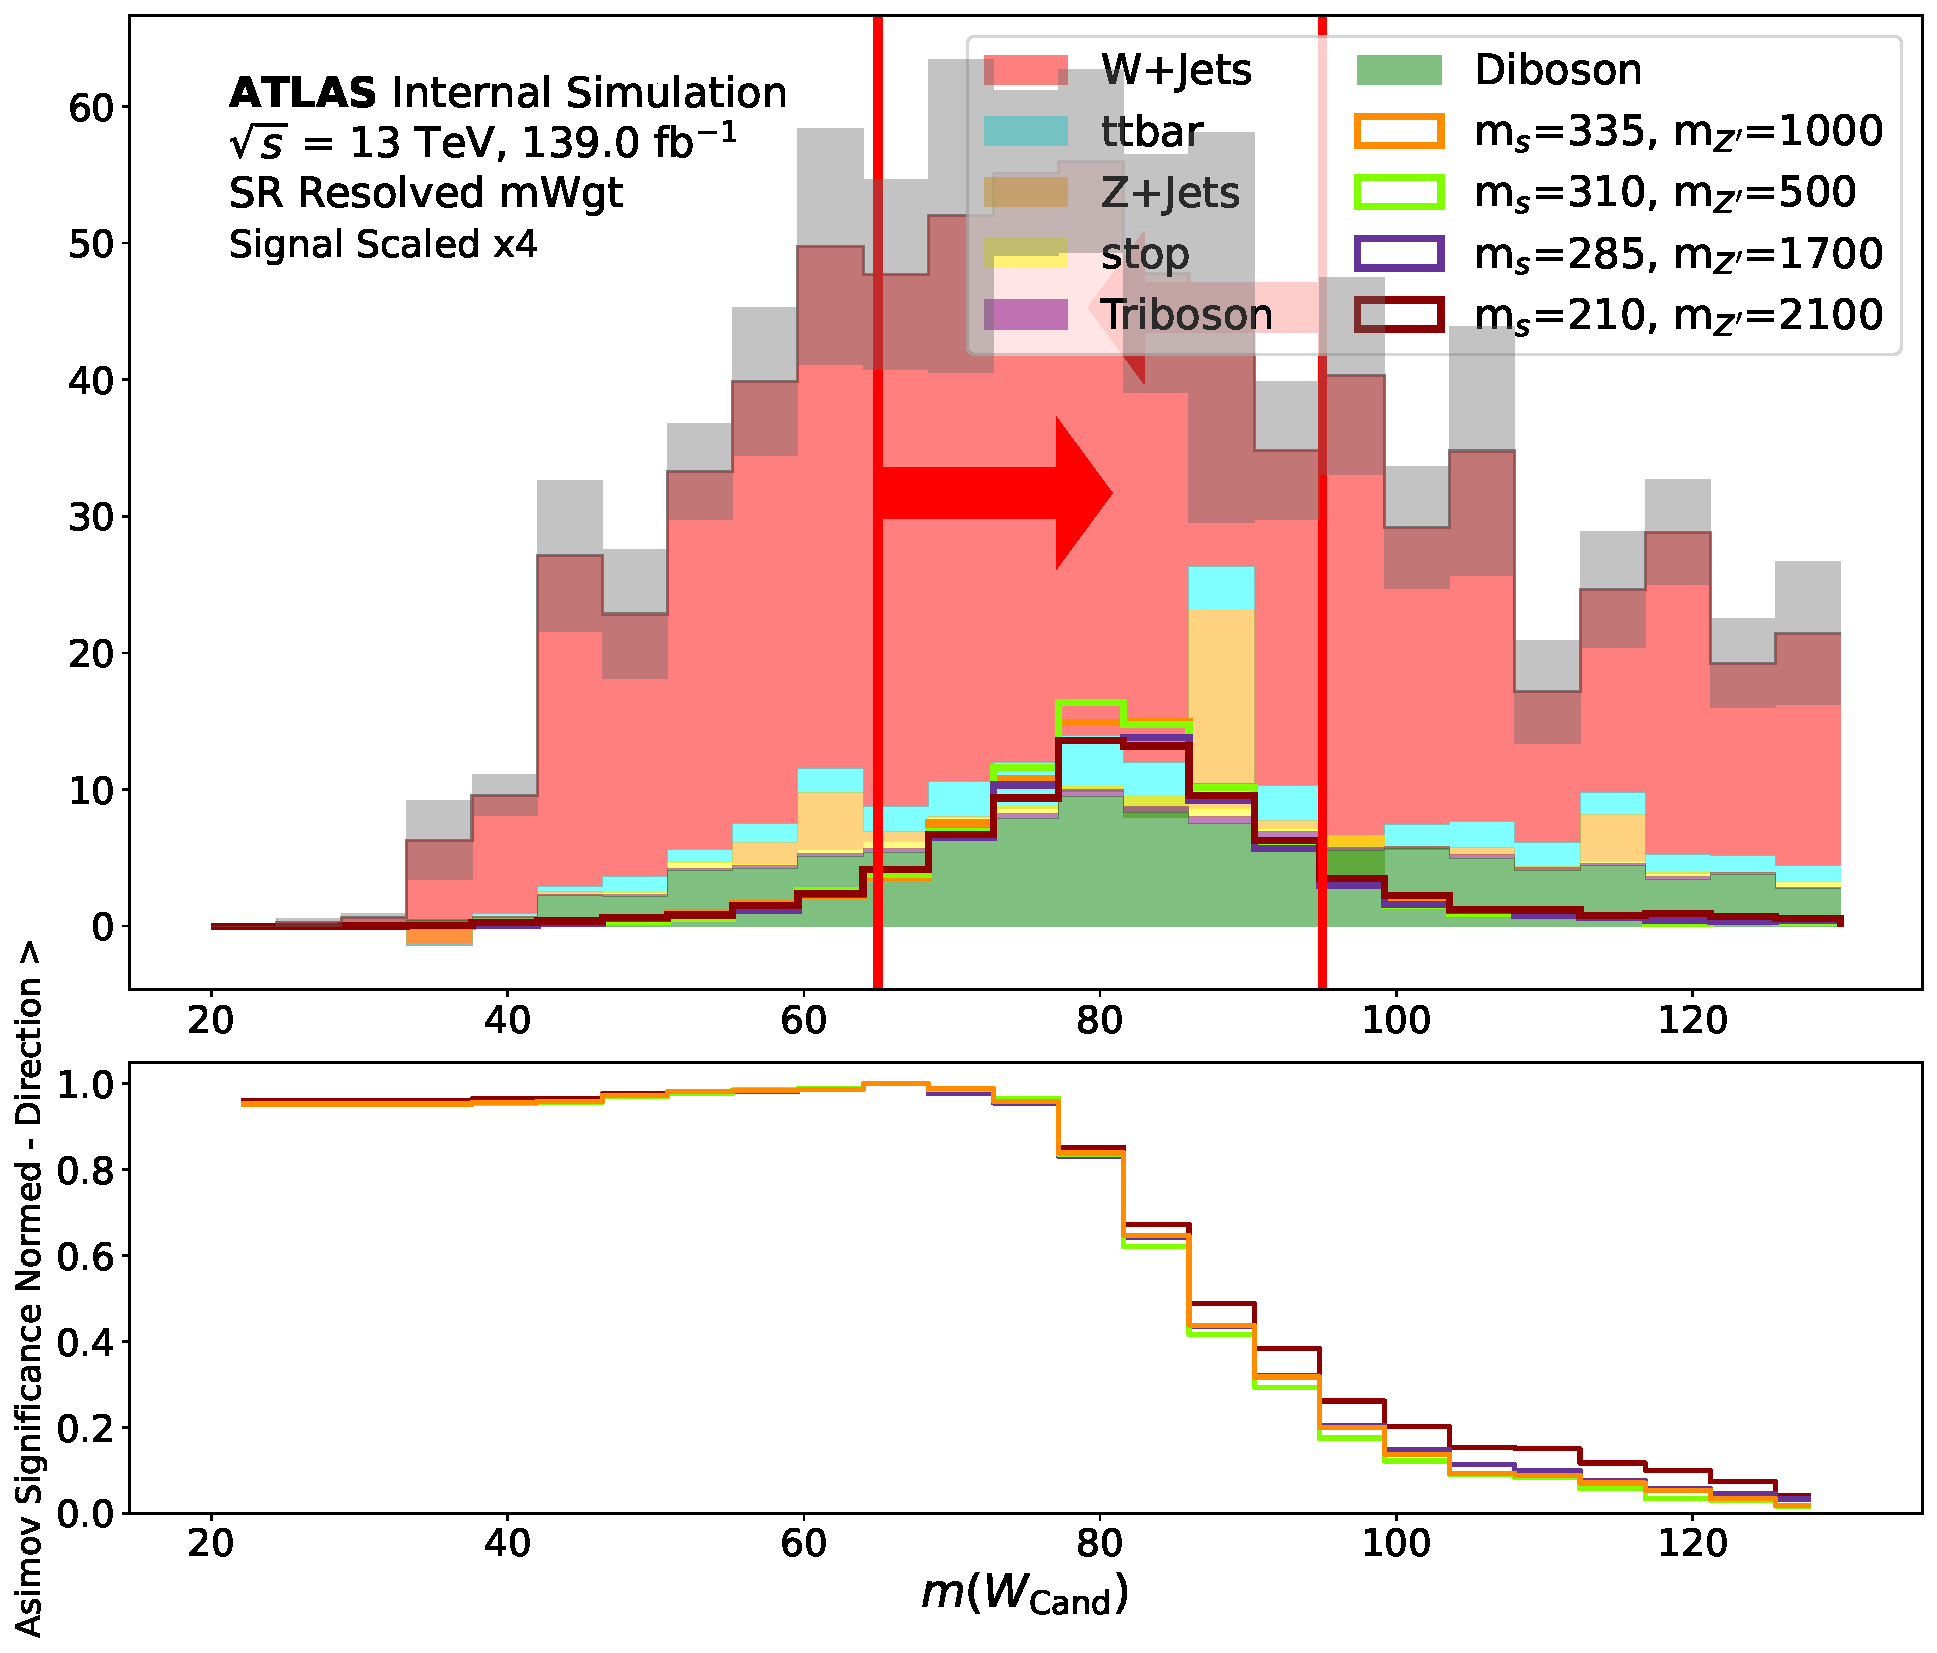
\includegraphics[width = 0.9\textwidth]{Figures/5/SR1L_Resolved_mWgt/WCand_m_normSig_N_1.pdf}
     \caption{\Wcandm Cut (\(Z\) evaluated for lower bound)}
    \end{subfigure}
    \begin{subfigure}[t]{0.48\textwidth}
    \centering
     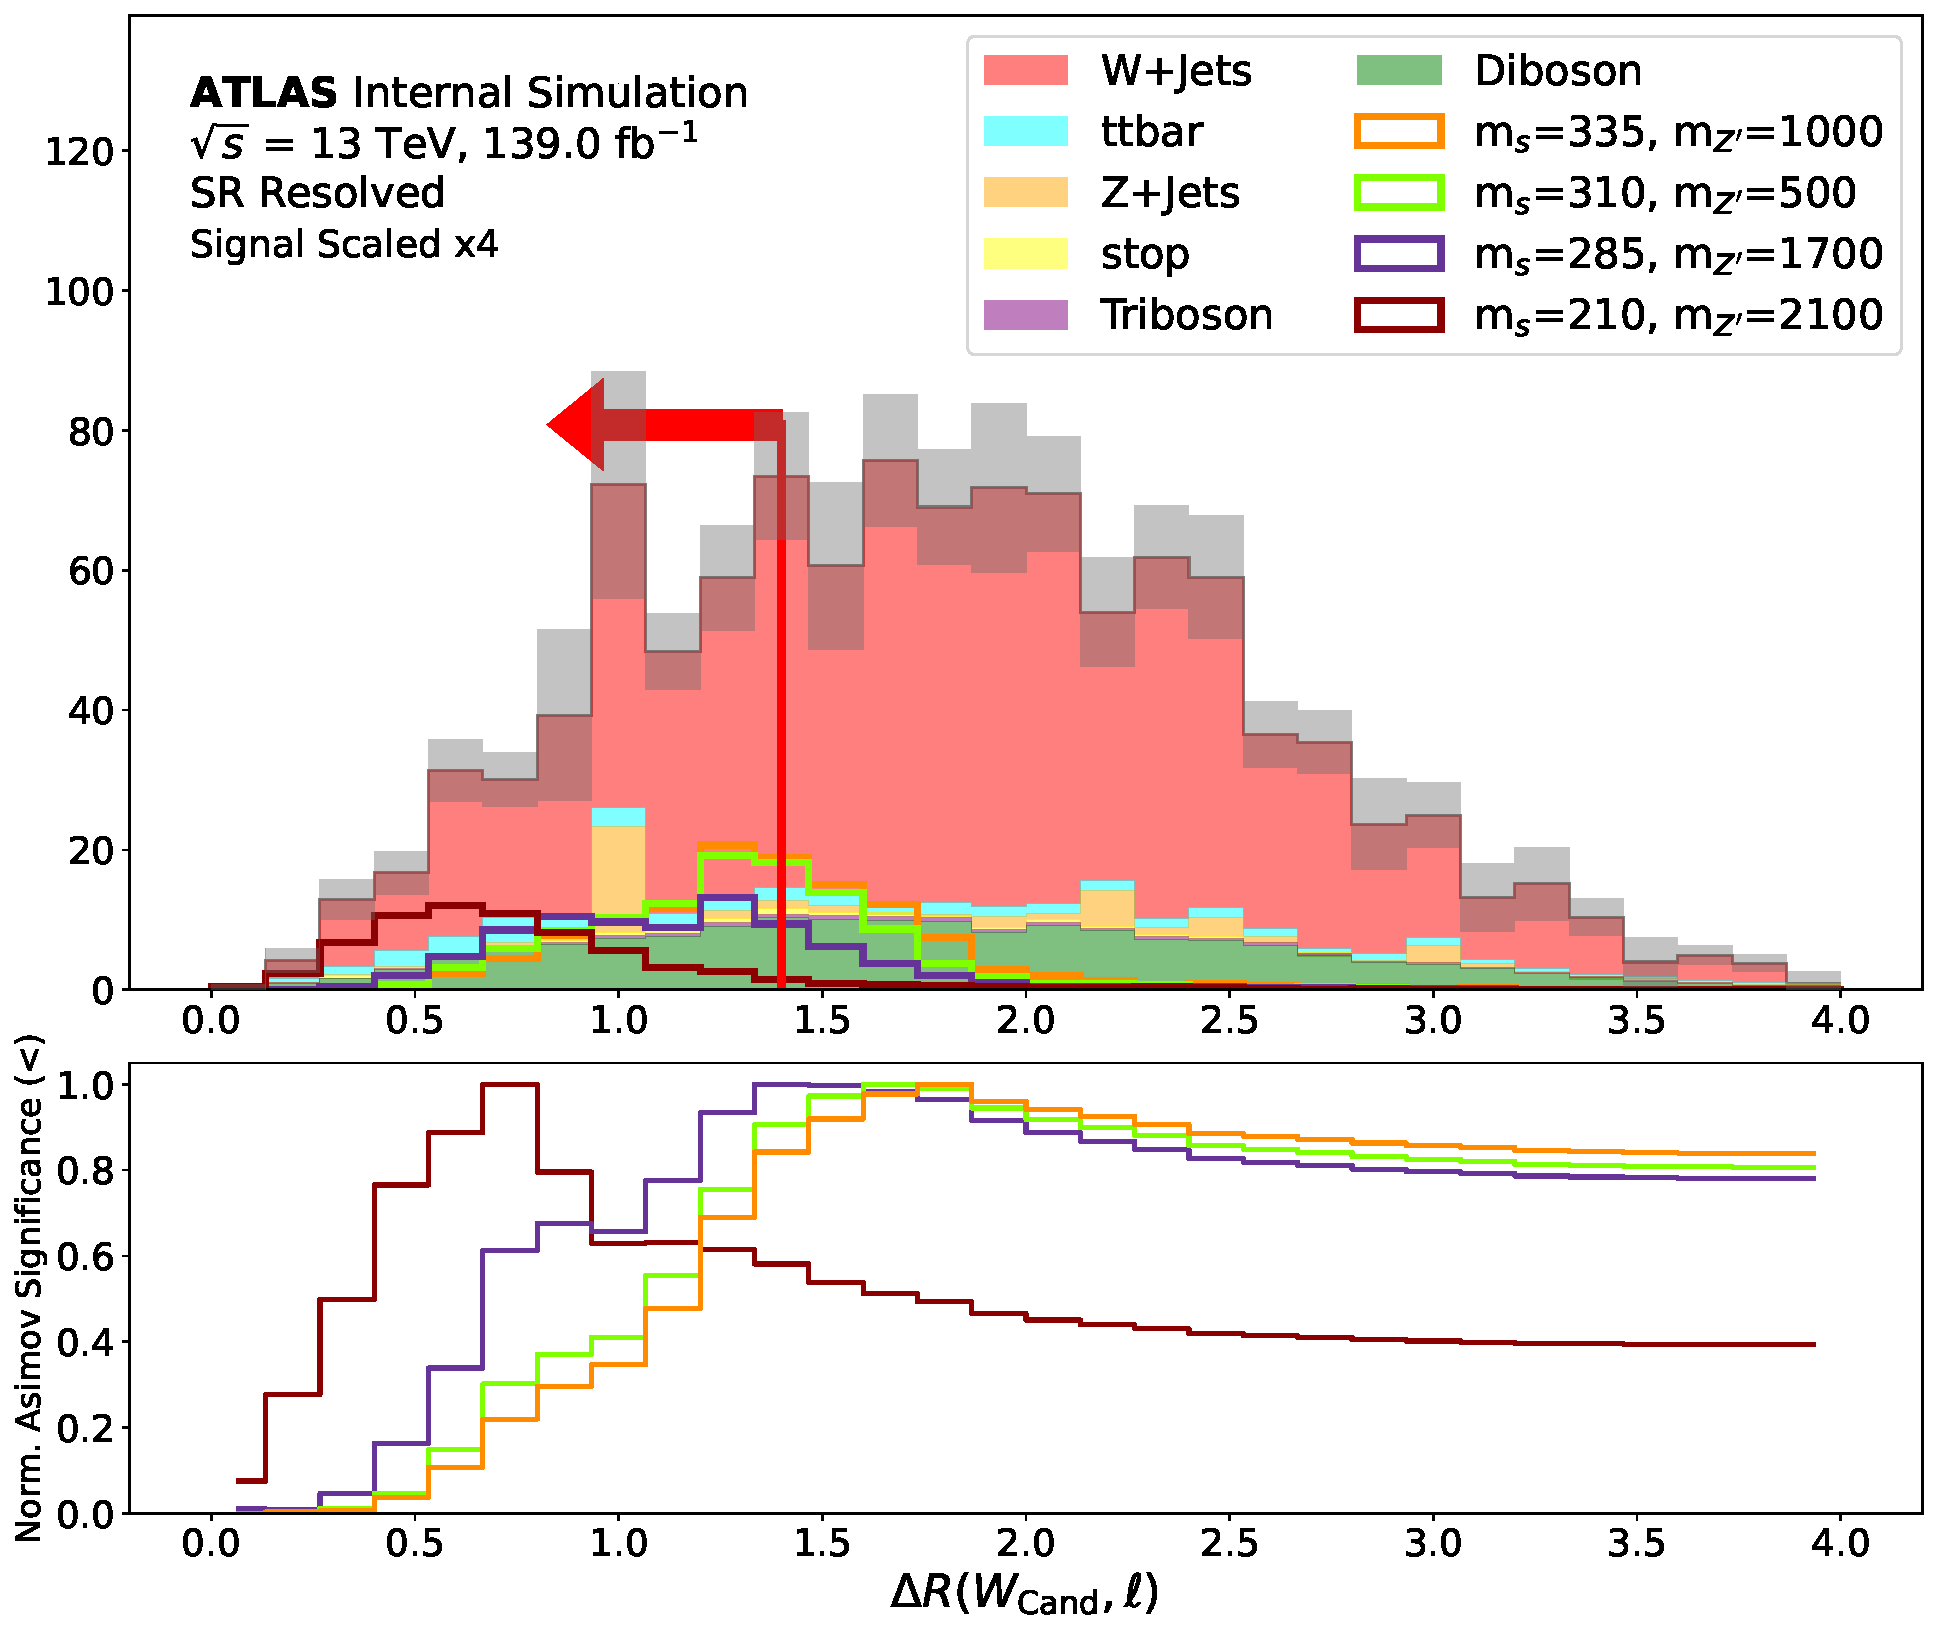
\includegraphics[width = 0.9\textwidth]{Figures/5/SR1L_Resolved/dRWl_normSig_N_1.pdf}
    \caption{\drWl}
    \end{subfigure}
%    \begin{subfigure}[t]{0.48\textwidth}
%    \centering
%     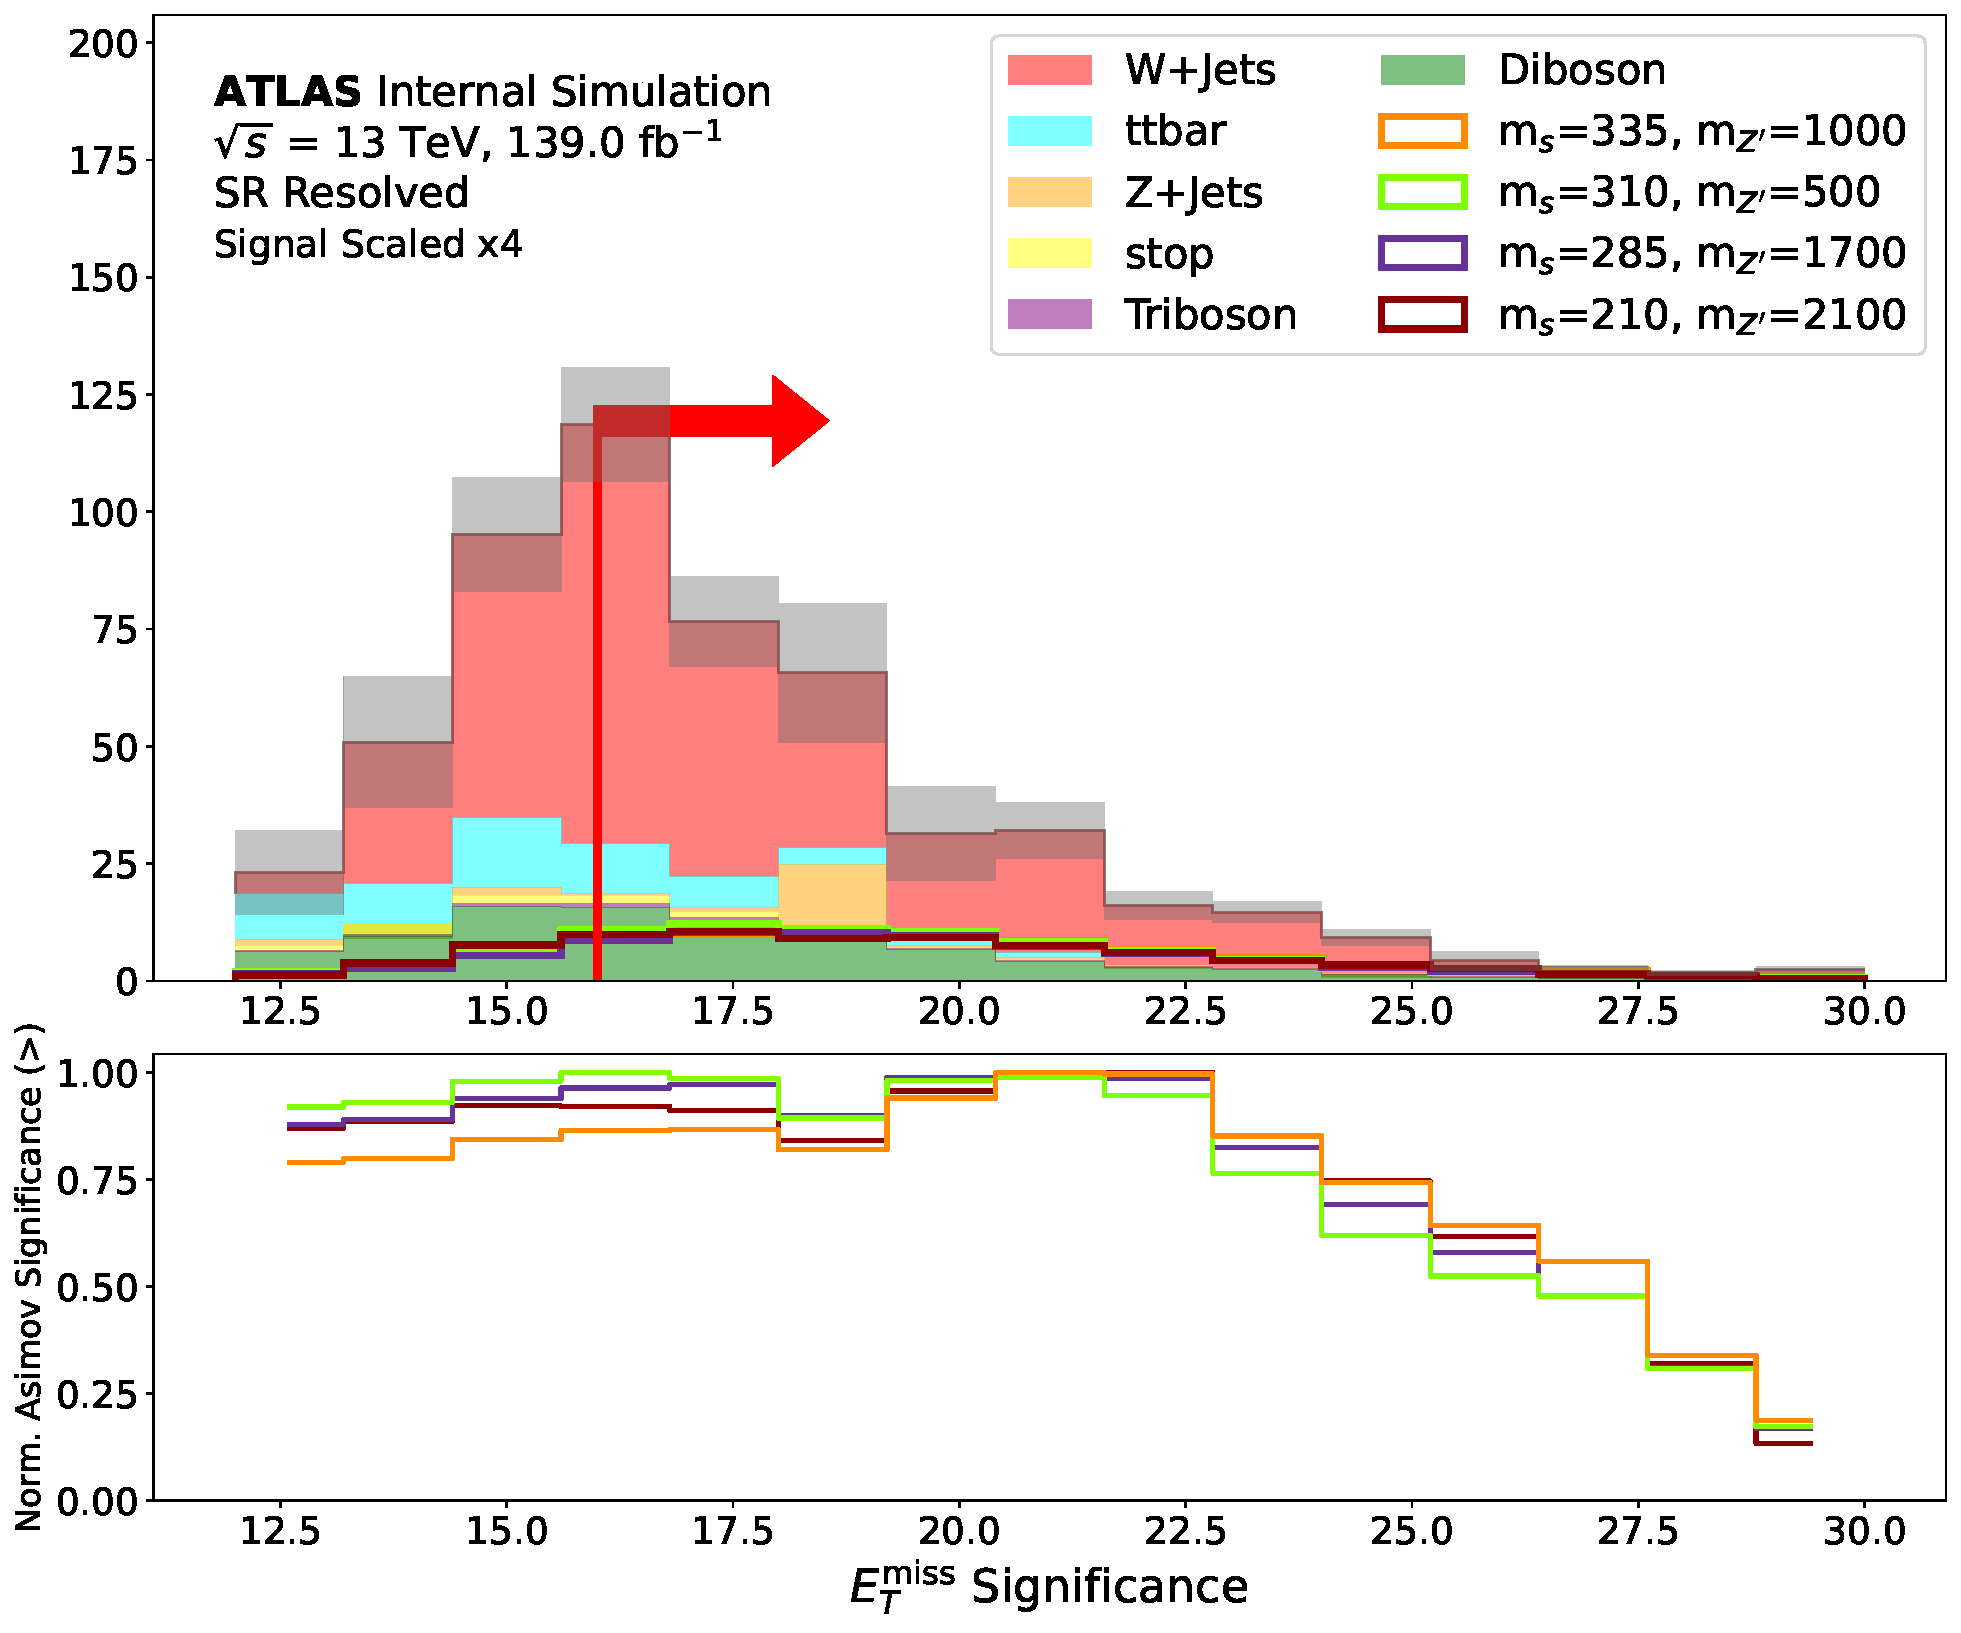
\includegraphics[width = 0.9\textwidth]{Figures/5/SR1L_Resolved/MetTST_Significance_normSig_N_1.pdf}
%    \caption{\metsig}
%    \end{subfigure}
%    \begin{subfigure}[t]{0.48\textwidth}
%    \centering
%     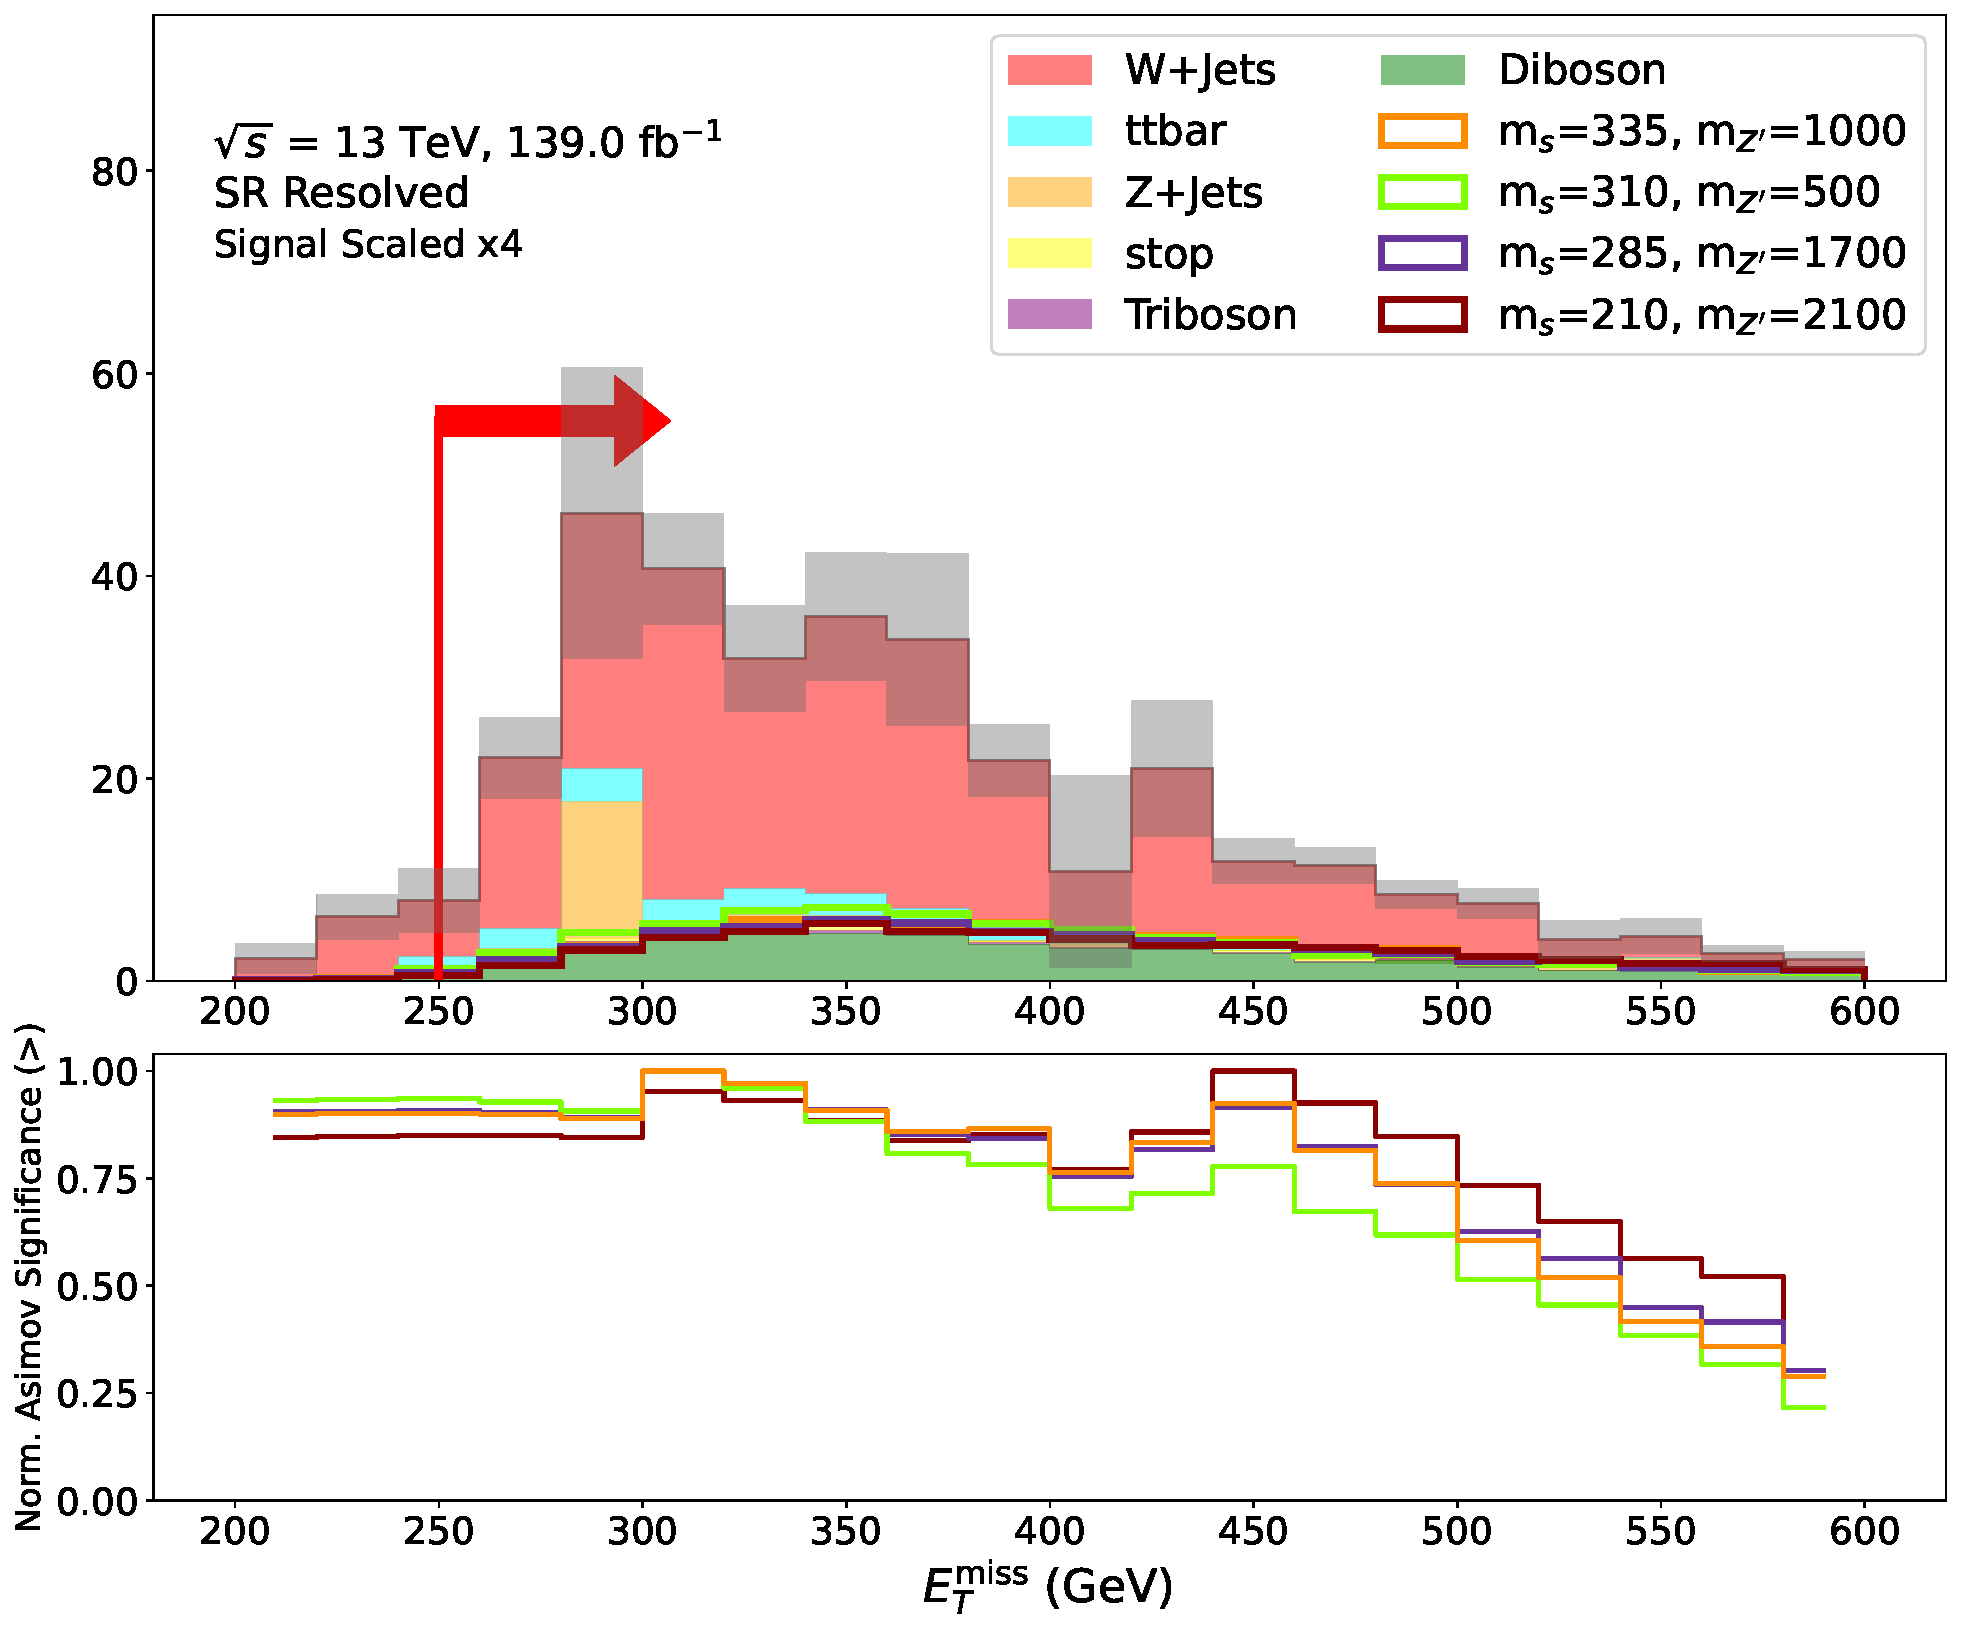
\includegraphics[width = 0.9\textwidth]{Figures/5/SR1L_Resolved/MetTST_met_normSig_N_1.pdf}
%    \caption{\met}
%    \end{subfigure}
     \caption[N-1 Distributions for the \Wcandm and \drWl variables used in the resolved signal region definition.]{N-1 Distributions for the \Wcandm and \drWl variables used in the resolved signal region definition. Grey bands show statistical uncertainty on the background estimate. The lower panel shows the cumulative Asimov significance normalized to unit peak, where the direction (\(>\) or \(<\)) specified in the y label indicates whether the significance is being summed from above (\(>\)) or from below (\(<\)). Red vertical line and arrow show placement and direction of selection on the given variable in this region.}
     \label{fig:Nminus1resolvedSR}
\end{figure}
%\begin{figure} \ContinuedFloat
%    \begin{subfigure}[t]{0.48\textwidth}
%    \centering
%     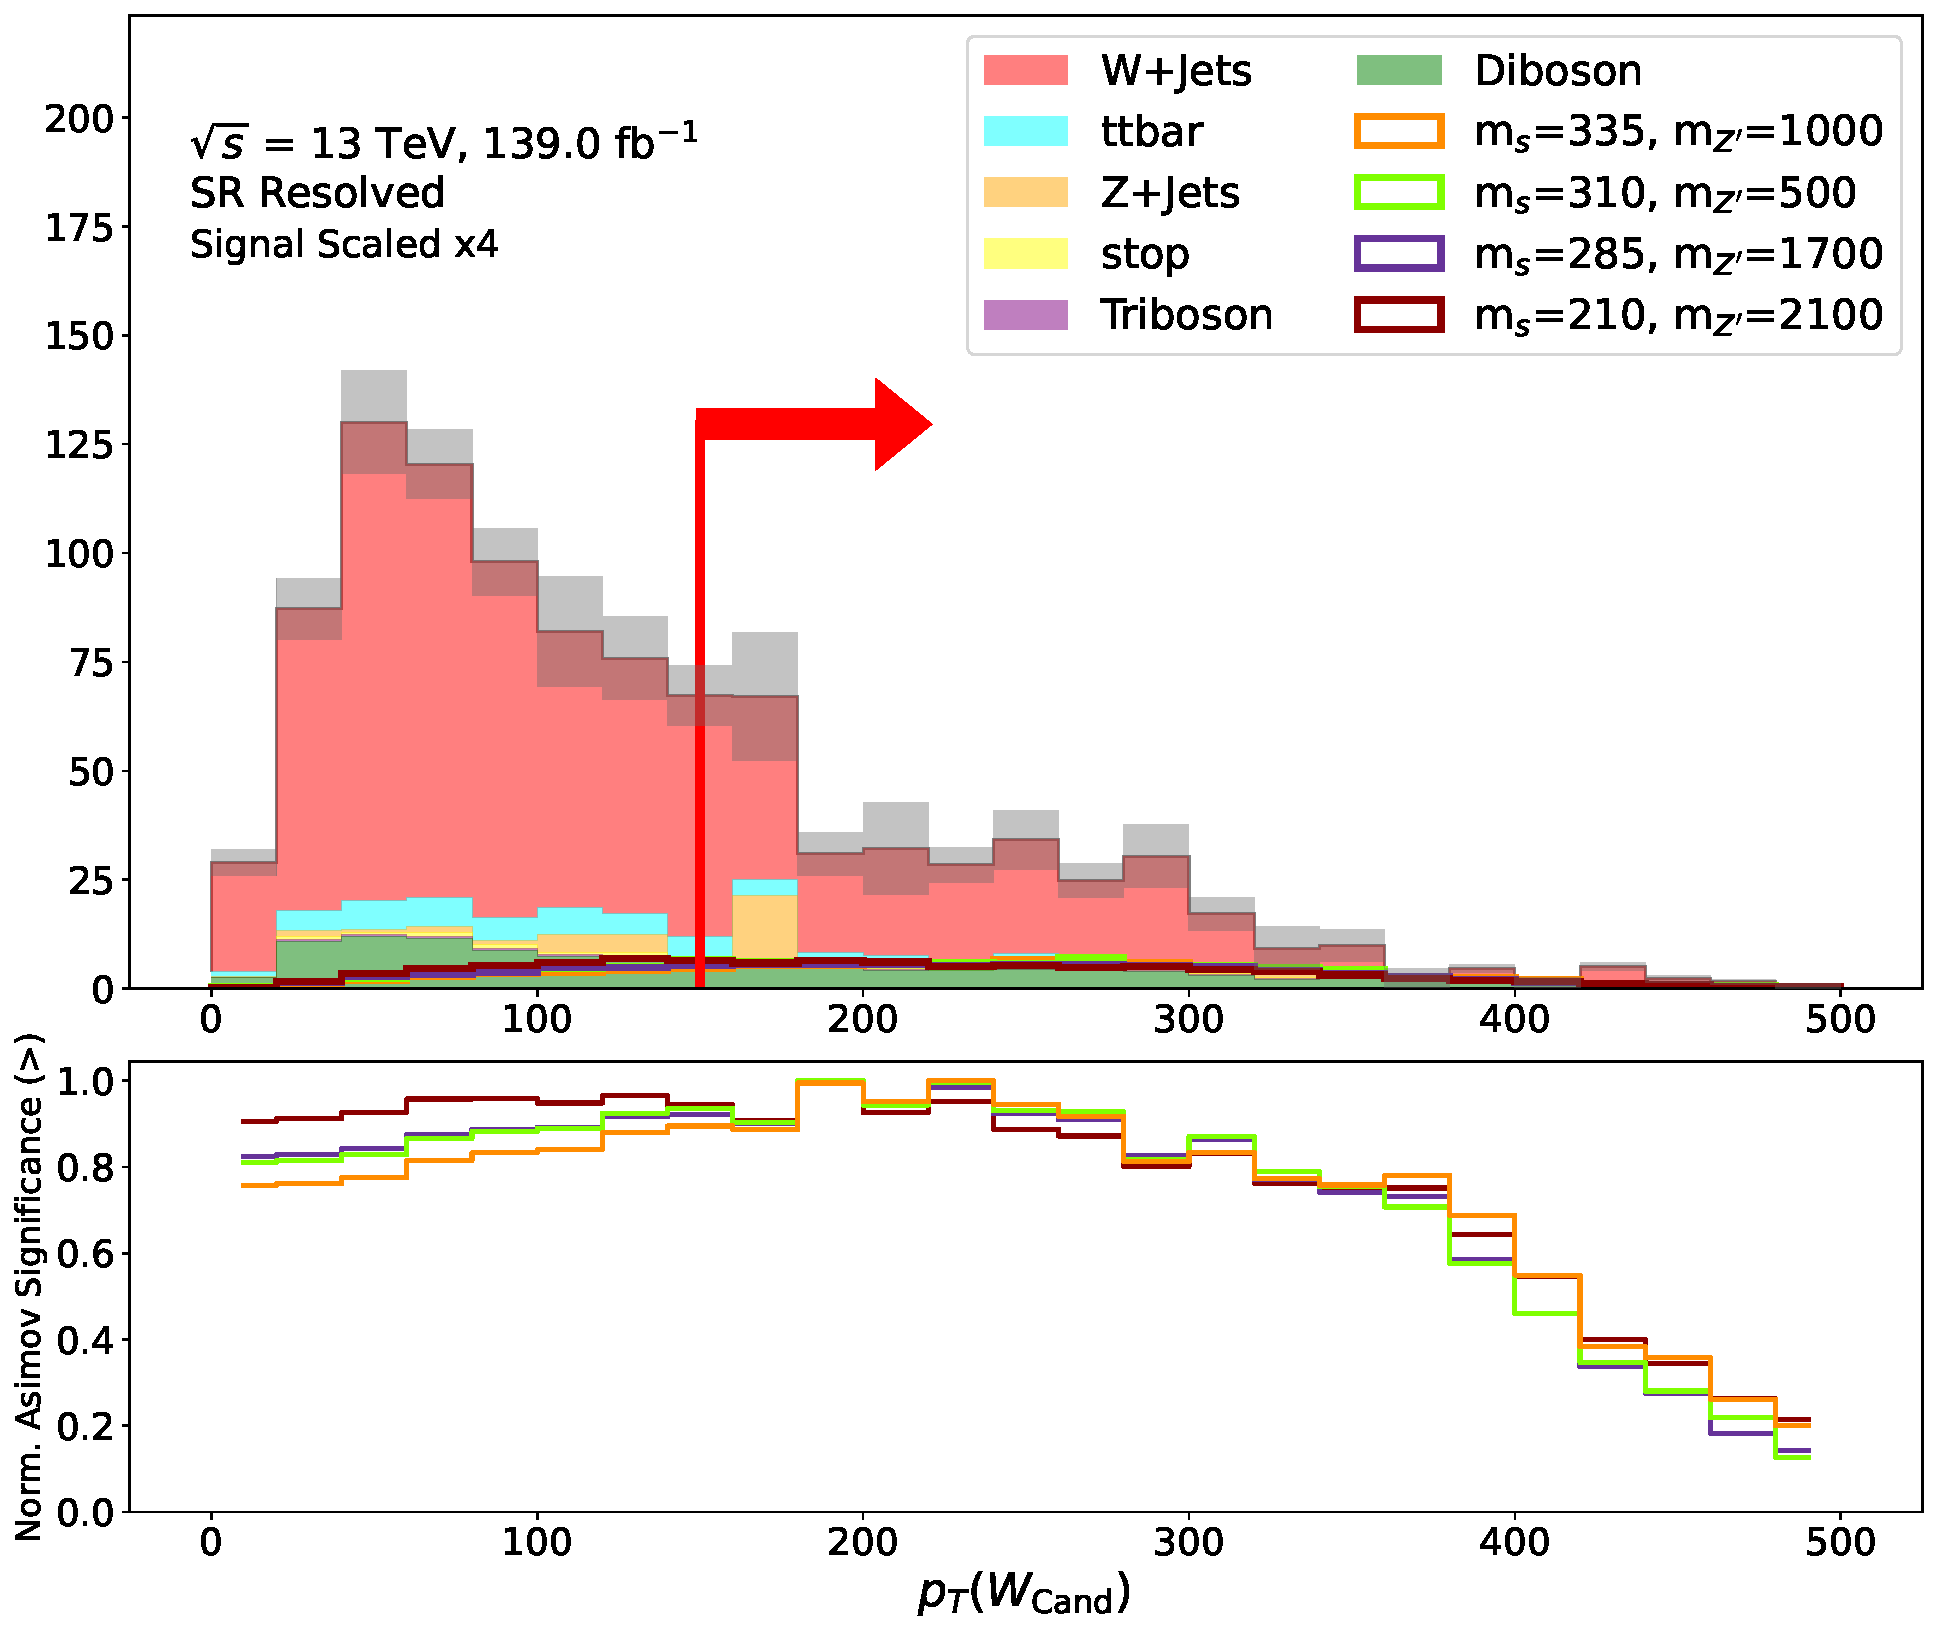
\includegraphics[width = 0.9\textwidth]{Figures/5/SR1L_Resolved/WCand_pt_normSig_N_1.pdf}
%    \caption{\Wcandpt}
%    \end{subfigure}
%     \caption{N-1 Distributions for selection requirements in the resolved signal region (continued)}
%  \end{figure}


\begin{table}[htbp]
  \centering
  \caption{Optimized selection criteria for the signal region in the merged and resolved categories.}
  \label{tab:SR_selection_opt}
  \begin{tabular}{l|l}
    \toprule
    \textbf{Merged Selection}  &  \textbf{Resolved Selection}  \\
    \midrule
    \midrule
    \multicolumn{2}{c}{Passes baseline selection} \\
     & Fails merged selection \\
    \(\NTAR>0\) & \(\Njets > 1\)  \\
    \(\mtlepmet>220~\GeV\) & \(\mtlepmet>200~\GeV\)\\
    \(\met>200~\GeV\) & \(\met>250~\GeV\)\\    
    \(\metsig>16\) & \(\metsig > 16\) \\
    \(68~\GeV < \mTAR < 89~\GeV\) & \(68~\GeV < \Wcandm < 89~\GeV\) \\
    \(\dRTARl<1.2\) &  \(\drWl  < 1.4\) \\
    \(\DtwoTAR<1.1\) &   \(\Wcandpt > 150~\GeV\) \\
    \bottomrule
  \end{tabular}
\end{table}

Tables \ref{tab:SR1L_Merged_bkg_cutflow} and  \ref{tab:SR1L_Resolved_bkg_cutflow} show the predicted yields of MC simulated events for the three dominant SM backgrounds after successive application of selections in the merged and resolved SRs respectively, beginning with the baseline selection. Tables \ref{tab:SR1L_Merged_bkg_cutflow} and  \ref{tab:SR1L_Resolved_bkg_cutflow} show the same information for the DH signal model at three sample mass points in \((\ms, \mZp)\).

\begin{table}[ht]
\caption[Cutflow yields after application of preselection cuts for the dominant SM backgrounds in the merged SR.]{\label{tab:SR1L_Merged_bkg_cutflow} Cutflow yields after application of preselection cuts for the dominant SM backgrounds in the merged SR. Percent passage is reported relative to the number of weighted events after application of the baseline selection.}
\begin{tabular}{l l l l }
\toprule
\textbf{Cut} & \textbf{W+jets} & \(\boldsymbol{t\bar{t}}\) & \textbf{Diboson}\tabularnewline
\midrule
\midrule
None & 11352445.72  & 101404110.82  & 1270378.37 \tabularnewline
\midrule
baseline selection & 93740.14 (100.00\%) & 51263.07 (100.00\%) & 8469.92 (100.00\%)\tabularnewline
\midrule
\(\NTAR \geq 1\) & 36957.80 (39.43\%) & 44993.63 (87.77\%) & 6887.00 (81.31\%)\tabularnewline
\midrule
\bjet veto & 34077.64 (36.35\%) & 5082.68 (9.91\%) & 6199.93 (73.20\%)\tabularnewline
\midrule
\(\mtlepmet > 220~\GeV\) & 21927.98 (23.39\%) & 2994.69 (5.84\%) & 3450.61 (40.74\%)\tabularnewline
\midrule
\(\mTAR \in (68, 89)~\GeV\)  & 942.31 (1.01\%) & 165.13 (0.32\%) & 206.63 (2.44\%)\tabularnewline
\midrule
\(\metsig > 16\)  & 437.27 (0.47\%) & 21.52 (0.04\%) & 85.00 (1.00\%)\tabularnewline
\midrule
\(\drTARl < 1.2\) & 65.79 (0.07\%) & 10.30 (0.02\%) & 21.46 (0.25\%)\tabularnewline
\midrule
\(\DtwoTAR < 1.1\) & 24.29 (0.03\%) & 4.29 (0.01\%) & 7.61 (0.09\%)\tabularnewline
\bottomrule
\end{tabular}
\end{table}

\begin{table}[ht]
\caption[Cutflow yields after application of preselection cuts for the dominant SM backgrounds in the resolved SR.]{\label{tab:SR1L_Resolved_bkg_cutflow} Cutflow yields after application of preselection cuts for the dominant SM backgrounds in the resolved SR. Percent passage is reported relative to the number of weighted events after application of the baseline selection.}
\begin{tabular}{l l l l }
\toprule
\textbf{Cut} & \textbf{W+jets} & \(\boldsymbol{t\bar{t}}\) & \textbf{Diboson}\tabularnewline
\midrule
\midrule
None & 11352445.72 & 101404110.82  & 1270378.37 \tabularnewline
\midrule
baseline selection & 93740.14 (100.00\%) & 51263.07 (100.00\%) & 8469.92 (100.00\%)\tabularnewline
\midrule
Fails merged selection & 93552.83 (99.80\%) & 51178.42 (99.83\%) & 8435.36 (99.59\%)\tabularnewline
\midrule
\(\Njets \geq 2\) & 41566.23 (44.34\%) & 49150.32 (95.88\%) & 6624.88 (78.22\%)\tabularnewline
\midrule
\bjet veto & 38106.85 (40.65\%) & 5696.57 (11.11\%) & 5888.39 (69.52\%)\tabularnewline
\midrule
\(\mtlepmet > 200~\GeV\) & 30794.06 (32.85\%) & 4053.26 (7.91\%) & 4045.52 (47.76\%)\tabularnewline
\midrule
\met \(>\) 250 ~\GeV & 14965.69 (15.97\%) & 1639.75 (3.20\%) & 2366.03 (27.93\%)\tabularnewline
\midrule
\(\Wcandm \in (65, 95)~\GeV\) & 5214.91 (5.56\%) & 816.93 (1.59\%) & 941.15 (11.11\%)\tabularnewline
\midrule
\(\metsig > 16\)  & 3041.82 (3.24\%) & 166.35 (0.32\%) & 429.93 (5.08\%)\tabularnewline
\midrule
\(\drWl < 1.4\) & 771.85 (0.82\%) & 58.37 (0.11\%) & 114.24 (1.35\%)\tabularnewline
\midrule
\(\Wcandpt > 150~\GeV\) & 242.64 (0.26\%) & 21.19 (0.04\%) & 51.12 (0.60\%)\tabularnewline
\bottomrule
\end{tabular}
\end{table}

\begin{table}[ht]
\caption[Cutflow yields for three sample signal points in the merged SR.]{\label{tab:SR1L_Merged_sig_cutflow} Cutflow yields after application of preselection cuts for three sample signal points in the merged SR. Signal points are labelled in column headers as (m\(_{Z'}\), m\(_s\)) (units of GeV). Percent passage is reported relative to the number of weighted events after application of the baseline selection.}
\begin{tabular}{l l l l }
\toprule
\textbf{Cut} & \textbf{(1000, 360)} & \textbf{(1700, 335)} & \textbf{(2100, 210)}\tabularnewline
\midrule
\midrule
None & 798.61 & 396.57 & 537.03   \tabularnewline
\midrule
baseline selection & 168.35 (100.00\%) & 111.66 (100.00\%) & 143.64 (100.00\%)\tabularnewline
\midrule
\(\NTAR \geq 1\) & 147.88 (87.84\%) & 98.12 (87.87\%) & 124.98 (87.01\%)\tabularnewline
\midrule
\bjet veto & 131.89 (78.34\%) & 87.51 (78.37\%) & 111.32 (77.50\%)\tabularnewline
\midrule
\(\mtlepmet > 220~\GeV\) & 102.83 (61.08\%) & 70.82 (63.42\%) & 92.86 (64.65\%)\tabularnewline
\midrule
\(\mTAR \in (68, 89)~\GeV\)  & 45.00 (26.73\%) & 30.85 (27.63\%) & 31.88 (22.19\%)\tabularnewline
\midrule
\(\metsig > 16\)  & 33.84 (20.10\%) & 23.97 (21.47\%) & 24.34 (16.95\%)\tabularnewline
\midrule
\(\drTARl < 1.2\) & 15.80 (9.39\%) & 13.33 (11.94\%) & 23.20 (16.15\%)\tabularnewline
\midrule
\(\DtwoTAR < 1.1\) & 11.10 (6.59\%) & 9.50 (8.51\%) & 16.19 (11.27\%)\tabularnewline
\bottomrule
\end{tabular}
\end{table}

\begin{table}[ht]
\caption[Cutflow yields for three sample signal points in the resolved SR.]{\label{tab:SR1L_Resolved_sig_cutflow} Cutflow yields after application of preselection cuts for three sample signal points in the resolved SR. Signal points are labelled in column headers as (m\(_{Z'}\), m\(_s\)) (units of GeV). Percent passage is reported relative to the number of weighted events after application of the baseline selection.}
\begin{tabular}{l l l l }
\toprule
\textbf{Cut} & \textbf{(1000, 360)} & \textbf{(1700, 335)} & \textbf{(2100, 210)}\tabularnewline
\midrule
\midrule
None & 798.61 & 396.57  & 537.03   \tabularnewline
\midrule
baseline selection & 168.35 (100.00\%) & 111.66 (100.00\%) & 143.64 (100.00\%)\tabularnewline
\midrule
Fails merged selection & 152.86 (90.80\%) & 100.58 (90.08\%) & 127.22 (88.57\%)\tabularnewline
\midrule
\(\Njets \geq 2\) & 138.08 (82.02\%) & 90.56 (81.10\%) & 110.52 (76.94\%)\tabularnewline
\midrule
\bjet veto & 121.13 (71.95\%) & 79.35 (71.06\%) & 96.14 (66.93\%)\tabularnewline
\midrule
\(\mtlepmet > 200~\GeV\) & 101.11 (60.06\%) & 68.49 (61.34\%) & 84.25 (58.65\%)\tabularnewline
\midrule
\met \(>\) 250 ~\GeV & 78.78 (46.80\%) & 55.43 (49.64\%) & 67.87 (47.25\%)\tabularnewline
\midrule
\(\Wcandm \in (65, 95)~\GeV\) & 55.87 (33.19\%) & 39.09 (35.01\%) & 42.40 (29.52\%)\tabularnewline
\midrule
\(\metsig > 16\)  & 40.37 (23.98\%) & 28.77 (25.77\%) & 29.22 (20.34\%)\tabularnewline
\midrule
\(\drWl < 1.4\) & 16.84 (10.00\%) & 14.51 (12.99\%) & 23.77 (16.55\%)\tabularnewline
\midrule
\(\Wcandpt > 150~\GeV\) & 13.35 (7.93\%) & 11.35 (10.16\%) & 15.87 (11.05\%)\tabularnewline
\bottomrule
\end{tabular}
\end{table}

\subsection{Control regions}
\label{sec:CRs}

There are in general numerous uncertain theoretical parameters involved in modelling signal and SM background processes produced by \(pp\) collisions at the LHC, and it is necessary to fix their values when generating the MC simulated events and weights used to predict the yields of these processes in the ATLAS collision data. These include, for example, parameters associated with the parton distribution function used to model the protons involved in the high-energy collisions. A recent review of progress in the determination of parton distribution functions can be found in Ref. \cite{PDF_determination_2013}, and recommendations for the evaluation of uncertainties associated with parton distribution function parameters in the context of studies performed with LHC data can be found in Ref. \cite{PDF4LHC_recos_2016}.

In some cases, the range of plausible choices for an uncertain parameter, or a set of related uncertain parameters, can produce an associated uncertain range of yield predictions that is non-negligible compared with the statistical yield uncertainties. The resulting uncertainties in predicted yields in the SR can be reduced by constraining the predicted yields using the ATLAS collision data in a kinematically similar region. 
%As presented in Chapter \ref{chapter:systematics}, so-called ``systematic uncertainties" are evaluated in these cases to quantify the systematic shifts in the predicted yields that would be induced by shifting specific parameters or sets of parameters within an acceptable range on the basis of existing theoretical or experimental constraints. 
%In addition, it is worth noting that since the SR selection is broadly optimized to maximize the yield of a BSM physics process relative to that of the known SM background processes, the SR by design occupies a relatively exclusive kinematic regime in which the parameter choices used for the MC event simulations have not necessarily have been validated extensively. In order to reduce the uncertainty of predicted yields in the SR arising from the particular choices of floating parameters in the MC simulations, it is desirable to constrain the predicted yields of major background processes in the SR as much as possible using the ATLAS collision data in a kinematically similar region. 

\wjets and \ttbar control regions (CRs), with enriched yields of these respective SM background processes, are defined in this search with the aim of providing data-driven constraints on the total yield of the \wjets and \ttbar backgrounds in the SRs within each of the merged and resolved kinematic categories. As discussed in detail in Section \ref{sec:fit_setup}, the data-driven constraints are obtained within each category by comparing the total yield of MC simulated SM background events to the observed yield of data in the CRs for the given category, and scaling the total predicted yield of the \wjets and \ttbar backgrounds in both the CRs and the SRs by multiplicative ``normalization factors", \(\mu_{\wjets, \text{category}}\) and \(\mu_{\ttbar, \text{category}}\), such that the total predicted yield of SM background processes within each control region is in close agreement with the observed yield of ATLAS collision data.

The selections for the \wjets and \ttbar CRs were designed with the following aims in order to provide effective and reliable constraints on the total yield of the respective SM background processes in the SR:

\begin{itemize}
\item To obtain a \textbf{high purity} of the background process of interest in the CR, as evaluated by its MC simulated yield in the CR relative to other MC simulated background processes. It is important that the predicted event yield in the CR be dominated by the background process of interest, to ensure that the ratio of total MC simulated yield from all SM background processes, \(\sum\limits_{\text{process }i} (N_\text{MC})_{i\text{, CR}}\) to the observed yield of ATLAS collision events \((N_\text{data})_\text{observed, CR}\) in the CR represents a reasonable approximation of the equivalent ratio for the background process \(p_\text{constraint}\) of interest:

\begin{equation}
\label{eq:cr_ratio}
\frac{\sum\limits_{\text{process }i} (N_\text{MC})_{i\text{, CR}}}{(N_\text{data})_\text{total observed, CR}} \approx \frac{(N_\text{MC})_{p_{\text{constraint}\text{, CR}}}}{(N_\text{data})_{p_\text{constaint}\text{, CR}}}
\end{equation}

\noindent where the index \(i\) runs over all simulated SM background processes.

\item The CR should contain a \textbf{relatively large number of MC simulated events} (and consequently a lower relative statistical uncertainty) for the background process of interest compared with the SR. This requirement is designed to ensure that the normalization factors \(\mu_{\wjets, \text{category}}\) and \(\mu_{\ttbar, \text{category}}\) will be constrained predominantly in the overall fit of MC simulated yields to the observed data (see Section \ref{sec:fit_setup} for details on the fitting strategy) by the comparison with data in the CRs, and also to minimize the statistical uncertainties of the fitted normalization factors associated with the limited number of MC simulated events in the CRs. 
\item To ensure \textbf{orthogonality with the SR}. In order for the CR to provide an unbiased data-driven constraint on the amplitude of a simulated SM background used in the signal region, it must be defined in such a way that no events are shared between these two regions.
\item To obtain a \textbf{negligibly small contamination of MC simulated signal events}. Negligible signal contamination is needed to ensure that the constraints on normalization factors are obtained purely from known physics processes in the data.
\item Events in the CR should occupy a \textbf{kinematic phase space that is as similar as possible to the SR}. This is important to ensure that the ratio of the MC simulated yield of SM background events to the observed yield of ATLAS collision data in the CR is representative of the equivalent ratio in the SR.
\end{itemize}

Table \ref{tab:CRs} summarizes the CRs used in the analysis and the cut changes relative to the SR that are used to define each CR. The CRs are discussed in more detail in Section \ref{sec:CRs}.

\begin{table}[htbp]
\centering
\caption{Summary of control regions.}
\label{tab:CRs}
\begin{tabular}{l l}
\toprule
\textbf{Control region}  & \textbf{Modified selections relative to the SR}  \\
\midrule
\midrule
\multirow{2}{*}{\textbf{Merged W+jets CR}} & \((\drTARl < 1.2) \rightarrow (\drTARl > 1.8)\) \\
						       & \((\metsig > 16) \rightarrow (\metsig > 12)\)  \\
\midrule
\textbf{Resolved W+jets CR}  &  \((\drWl < 1.4) \rightarrow (\drWl > 1.4)\) \\
\midrule
\multirow{2}{*}{\textbf{Merged }\(\boldsymbol{t\bar{t}}\)\textbf{ CR}} & \((\text{N(b-tagged jets)} < 1) \rightarrow \text{N(b-tagged jets)} \geq 2\)  \\
						       & \((\metsig > 16) \rightarrow (\metsig > 12)\)  \\
\midrule
\textbf{\textbf{Resolved }\(\boldsymbol{t\bar{t}}\)\textbf{ CR}} & \((\text{N(b-tagged jets)} < 1) \rightarrow \text{N(b-tagged jets)} \geq 2\)  \\
\bottomrule
\end{tabular}
\end{table}

\subsubsection{\wjets Control Region Definition}
\label{sec:wjets_CR_defn}

A \wjets CR (a.k.a. CRW) is defined to obtain a high purity and yield of the \wjets background process by reversing the cut on \DeltaR(W, \(\ell\)). Orthogonality with the SR is ensured by the reversal of the \DeltaR(W, \(\ell\)) cut. The lower bound on \met significance is also reduced to 12 in the merged category of the CR in order to reduce the relative statistical uncertainty by boosting the number of MC simulated events in the region. In addition, after some study the cut on \DeltaR(W, \(\ell\)) in the merged CRW was tightened from a simple reversal - \((\drTARl < 1.2) \rightarrow (\drTARl > 1.2)\) - to a slightly increased lower bound of (\(\drTARl > 1.8\)) in order to reduce the predicted yield of signal processes in the CR to an acceptable level.

The motivation for reversing the \DeltaR selection is that, as shown schematically in Figure \ref{fig:CRW_topology}, a \DeltaR reversal would largely reverse the directions of the lepton and neutrino in the \wjets process described in Section \ref{sec:wjets_description}, without modifying the kinematic details of the hadronic activity that fakes a hadronically-decaying \(W\) candidate for this process in the SR. As a result, the modelling of \wjets events in this \DeltaR-reversed region would be expected to be similar to \wjets events in the SR, with the exception of the reversed lepton and neutrino directions in the \(W\rightarrow\ell\nu\) decay.

\begin{figure}[htbp]
  \centering
  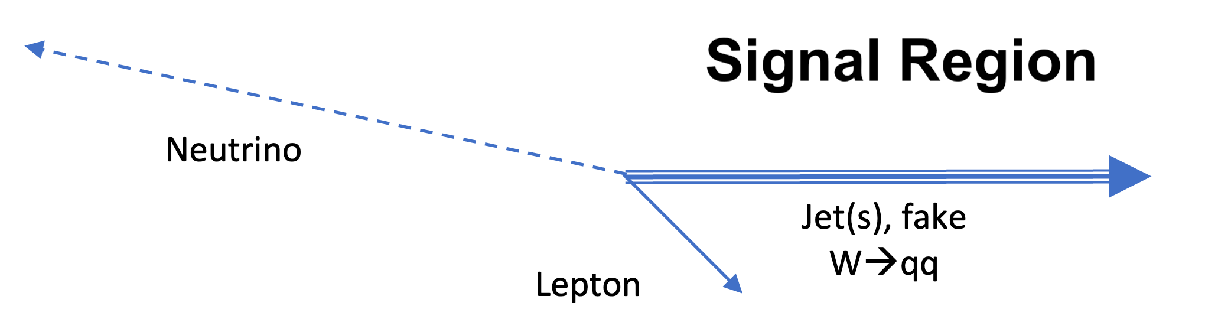
\includegraphics[width=0.49\textwidth]{Figures/5/SR_topology.pdf}
  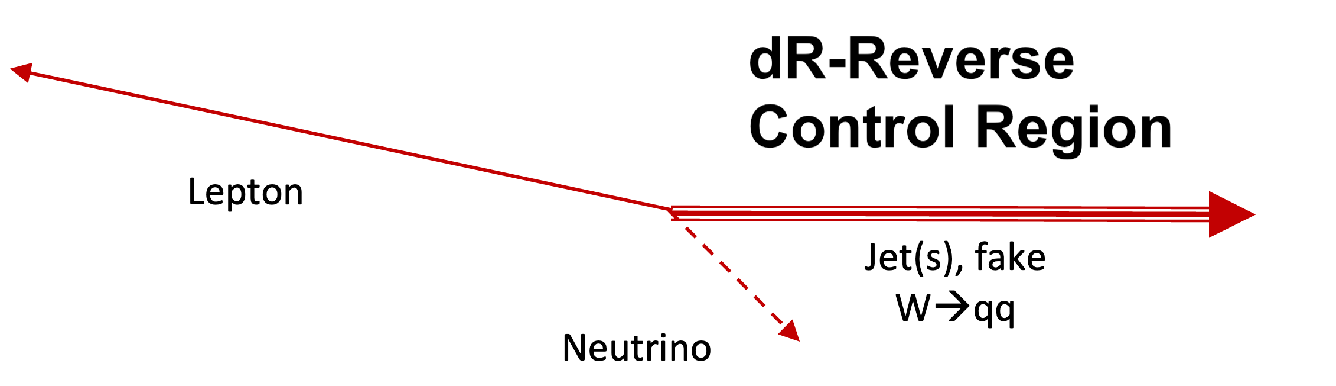
\includegraphics[width=0.49\textwidth]{Figures/5/CRW_topology.pdf}
  \caption[Comparison of typical event topologies between the signal region and the \wjets control region.]{Comparison of typical event topologies between the SR and the \wjets CR, showing that the typical directions of the lepton and neutrino relative to hadronic activity faking the hadronically-decaying \(W\) boson are simply reversed.}
  \label{fig:CRW_topology}
\end{figure}

Kinematic distributions of interest are compared between the \wjets CRs and the SRs in Figures \ref{fig:N_1_CRW_merged} and \ref{fig:N_1_CRW_resolved} in Appendix \ref{app:appendix_SR_CR_distributions_wjets}. 

A comparison of the \met distributions between the merged SR and CRW in Figures \ref{fig:N_1_SR_merged_met} and \ref{fig:N_1_CRW_merged_met} indicates some bias towards lower \met for events that pass the merged CRW selection. This difference is attributable to two factors. First, because the \metsig is in general expected to be positively correlated with \met, the loosened \metsig cut of \(\metsig>12\) in the merged CRW compared with \(\metsig>16\) in the SR would be expected to allow a larger proportion of low-\met events into the region. The impact of the loosened \metsig selection in the merged CRW is shown in Figure \ref{fig:N_1_SR_CRW_merged_metsig} by comparing the \met distribution between the merged SR and the merged CRW, either with or without the loosened \metsig selection in the merged CRW. Tightening the \metsig lower bound is seen to remove most of the low-\met bias in the merged CRW. The small remaining bias towards low \met in the merged CRW even after tightening the \metsig selection is attributed to the expected reversal of the neutrino direction in the \DeltaR-reversed topology of \wjets background in the CRW, such that it becomes approximately aligned with the high-pt TAR jet rather than recoiling against both the TAR jet and the lepton. The neutrino \pt required to conserve momentum in the \DeltaR-reversed topology will on average be somewhat smaller due to the approximately opposing momenta of the lepton and the TAR jet. Since the neutrino constitutes the only source of true \met in the \wjets background, this implies that the \met distribution would be expected to become somewhat biased to lower values in the CRW topology, as observed. 

 \begin{figure}[htbp]
    \begin{subfigure}[t]{0.48\textwidth}
    \centering
     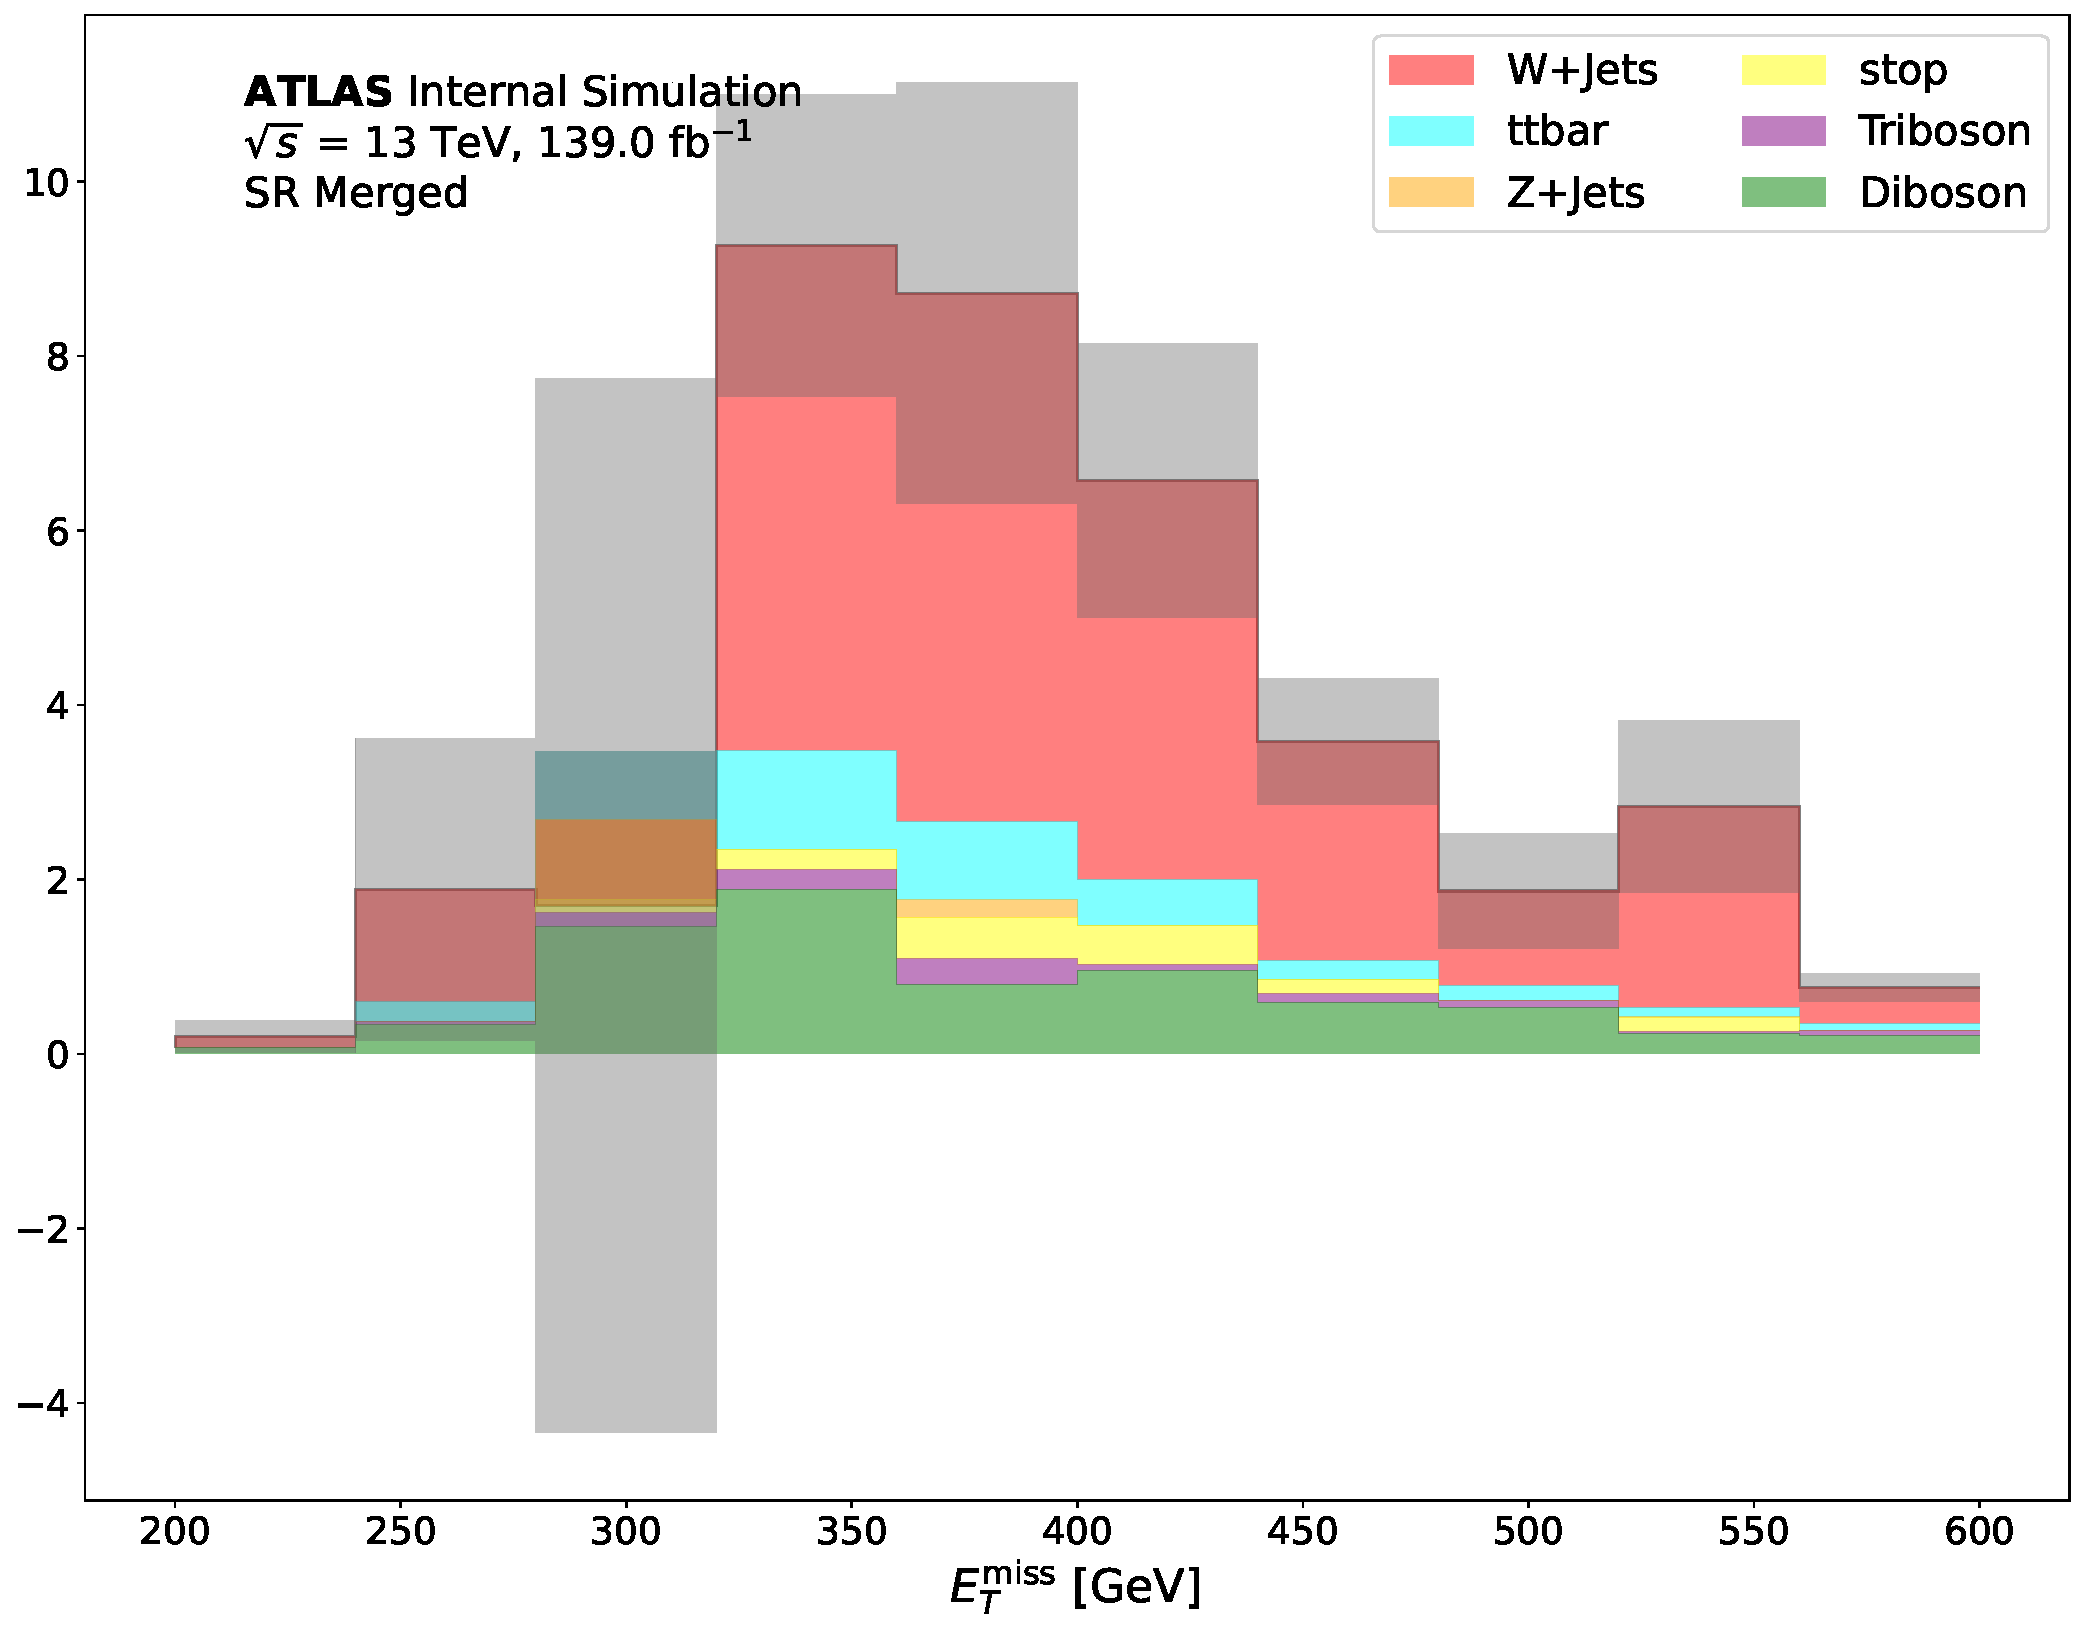
\includegraphics[width = 0.99\textwidth]{Figures/App_SR_CR_distributions/SR1L_Merged/MetTST_met_N_1.pdf}
    \caption{merged SR}
    \end{subfigure}
    \begin{subfigure}[t]{0.48\textwidth}
    \centering
     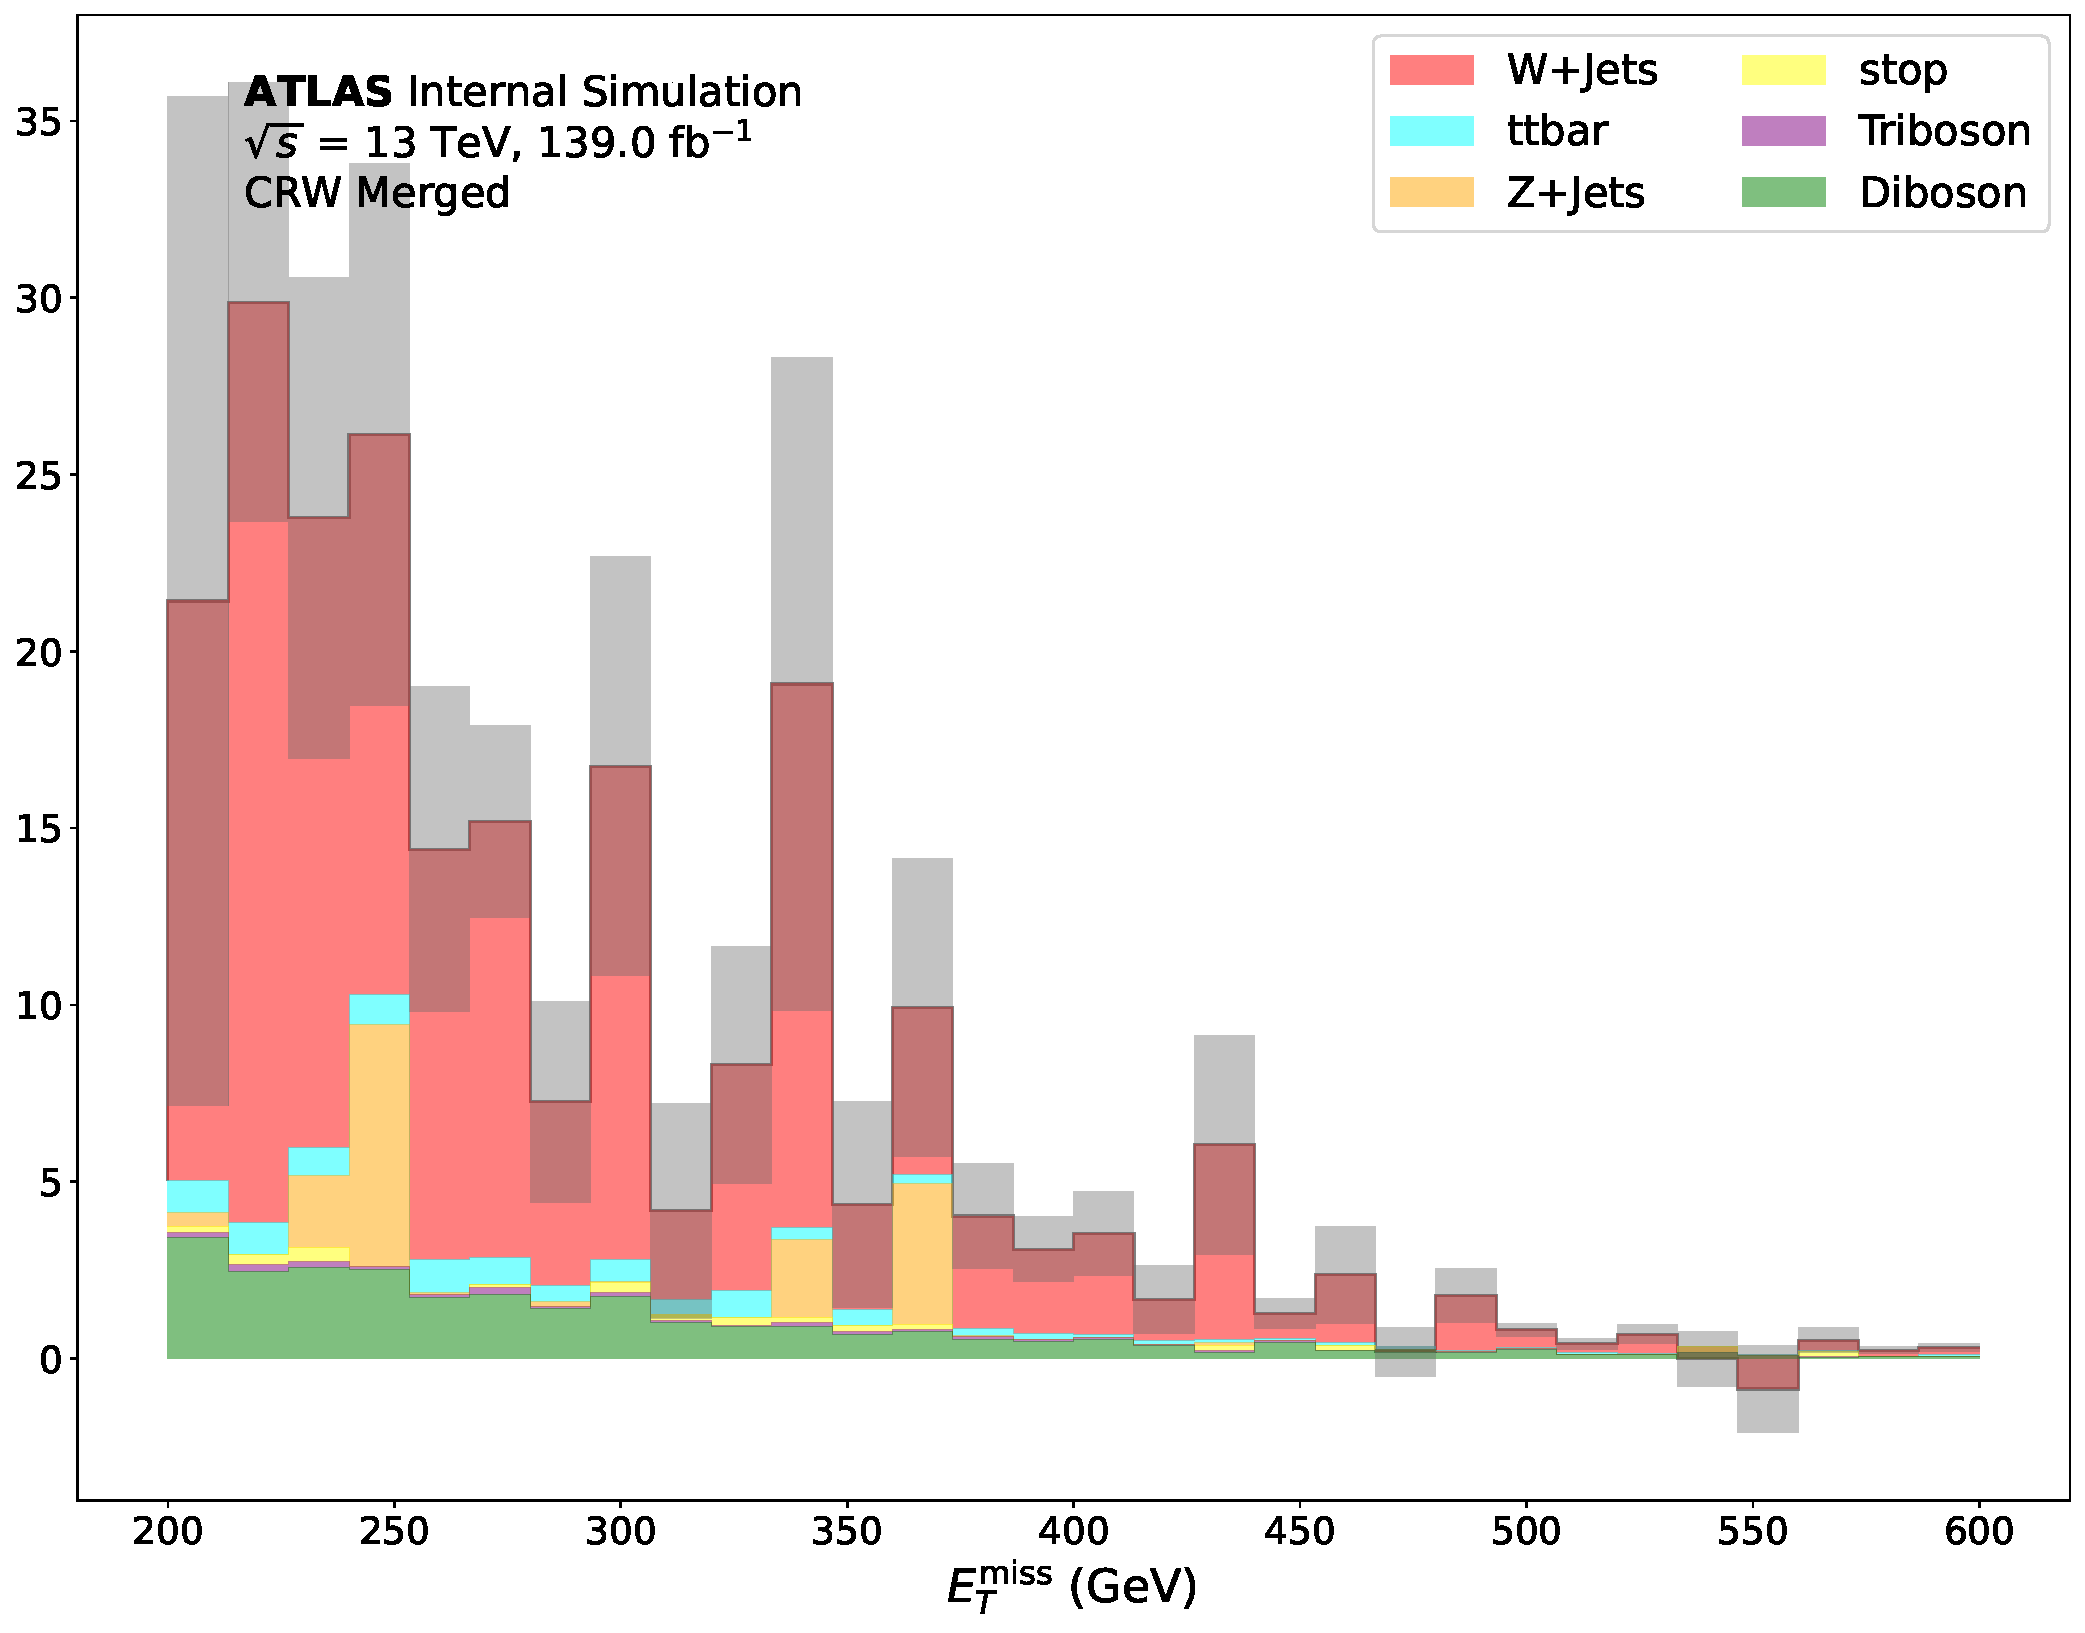
\includegraphics[width = 0.99\textwidth]{Figures/App_SR_CR_distributions/CRW_Merged/MetTST_met_N_1.pdf}
    \caption{merged CRW (\(\metsig>12\))}
    \end{subfigure}
    \begin{subfigure}[t]{\textwidth}
    \centering
     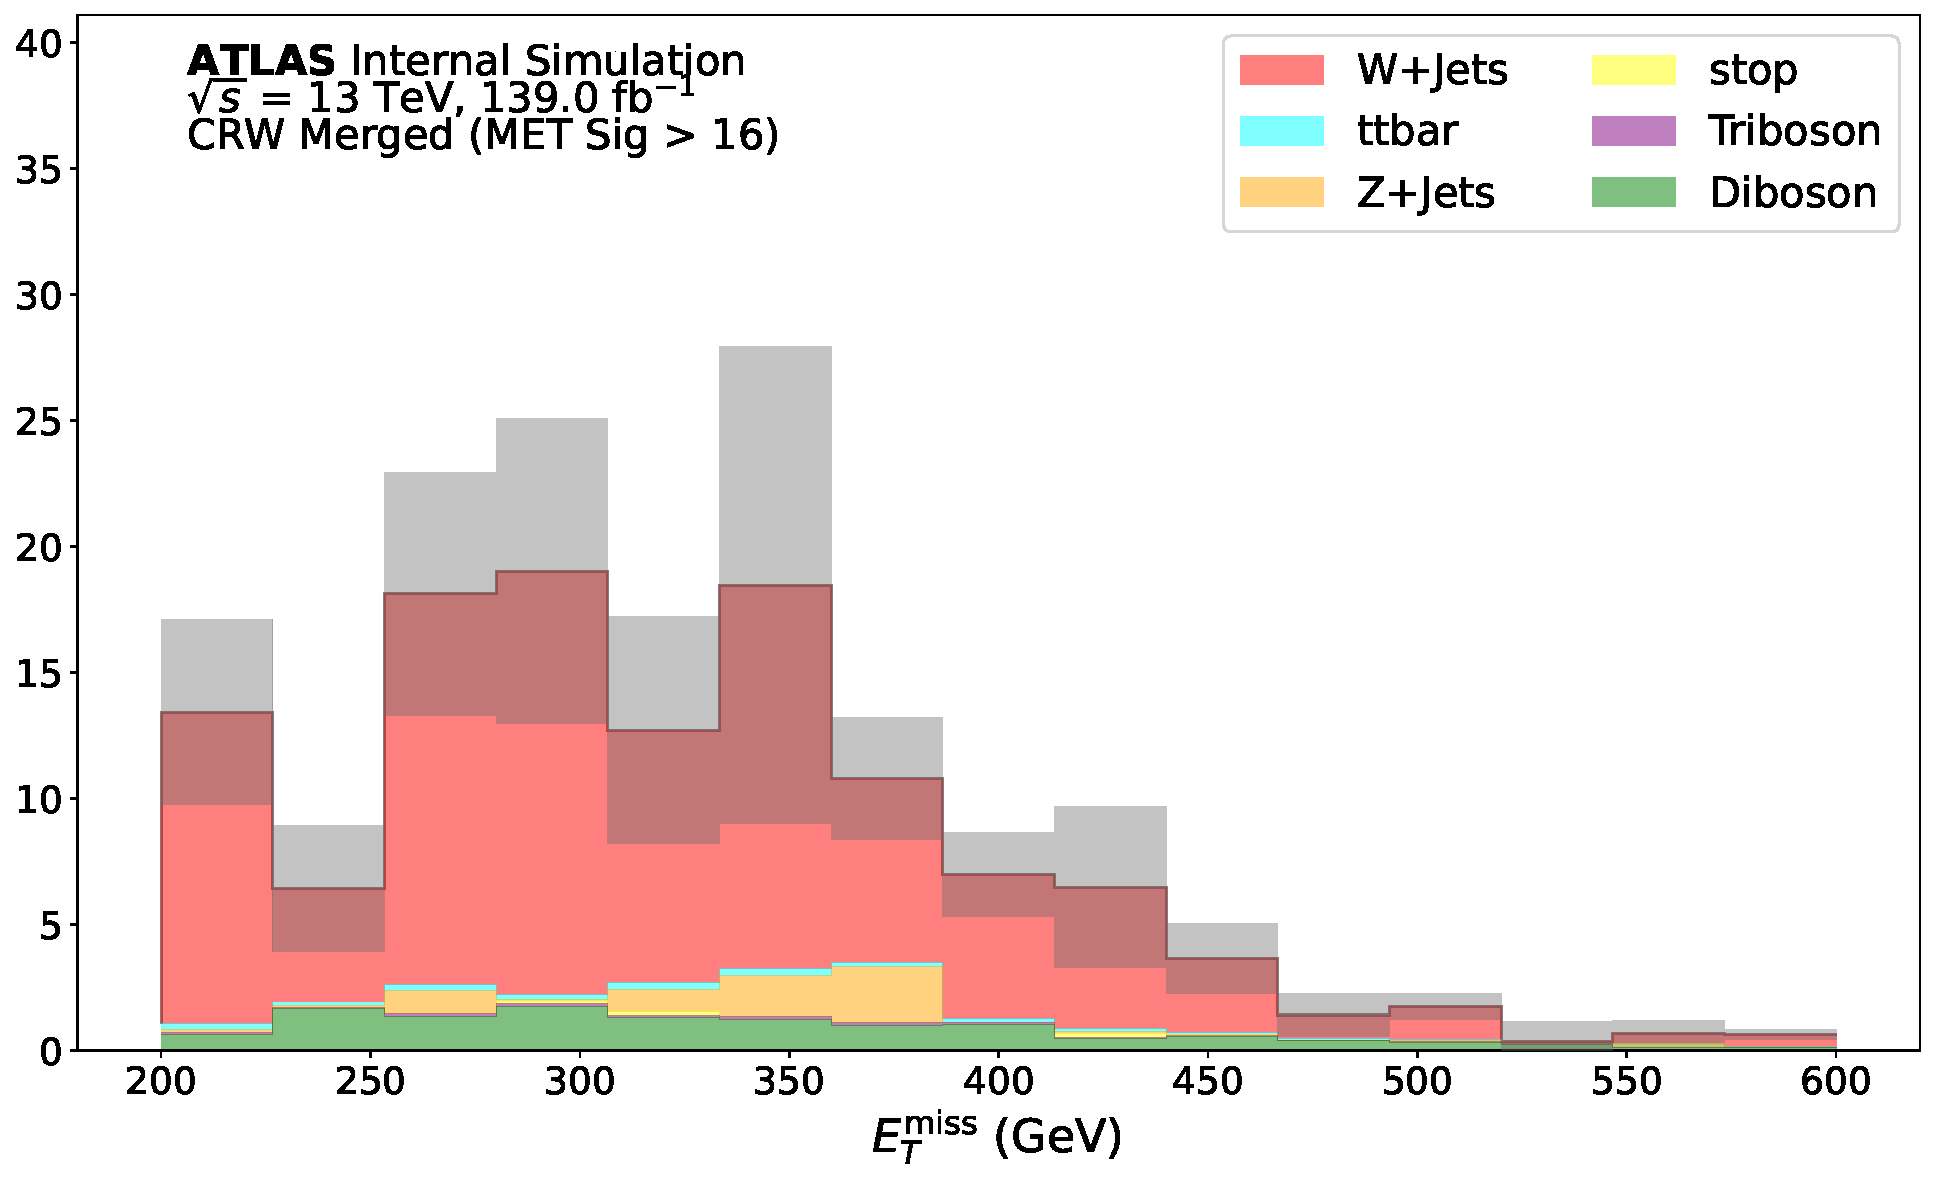
\includegraphics[width = 0.48\textwidth]{Figures/5/MetTST_met_N_1_CRW_metsig_gt_16.pdf}
    \caption{merged CRW (\(\metsig>16\))}
    \end{subfigure}
    \caption[Comparison of N-1 distributions between the merged signal region and the merged \wjets control region, for different lower bounds on \metsig in the merged signal region.]{Comparison of N-1 distributions between the merged SR (top left) and the merged CRW, with the lower bound on \metsig in the merged CRW either kept at its nominal value of 12 (upper right), or tightened (bottom) to match the \(\metsig>16\) cut applied in the merged SR. }
    \label{fig:N_1_SR_CRW_merged_metsig}
  \end{figure}

A comparison of Figures \ref{fig:N_1_SR_merged_met} and \ref{fig:N_1_CRW_merged_met} shows that, though present, this bias in the \met distribution is much more subtle in the resolved SR. This is attributed to the fact that the lower bound on \metsig is not loosened compared with the SR in the resolved category, in addition to the relatively low \pt of the hadronic activity that the neutrino is approximately aligned with in the CRW. 

Based on the comparable shapes of the other kinematic distributions in the merged and resolved categories, it is concluded that the kinematics of events in the \wjets CRs are sufficiently similar to those in the SR of the corresponding category that the constraints on normalization of the \wjets background evaluated in the \wjets CRs can be reasonably applied in the SR. 

%\begin{figure}[htbp]
%  \centering
%    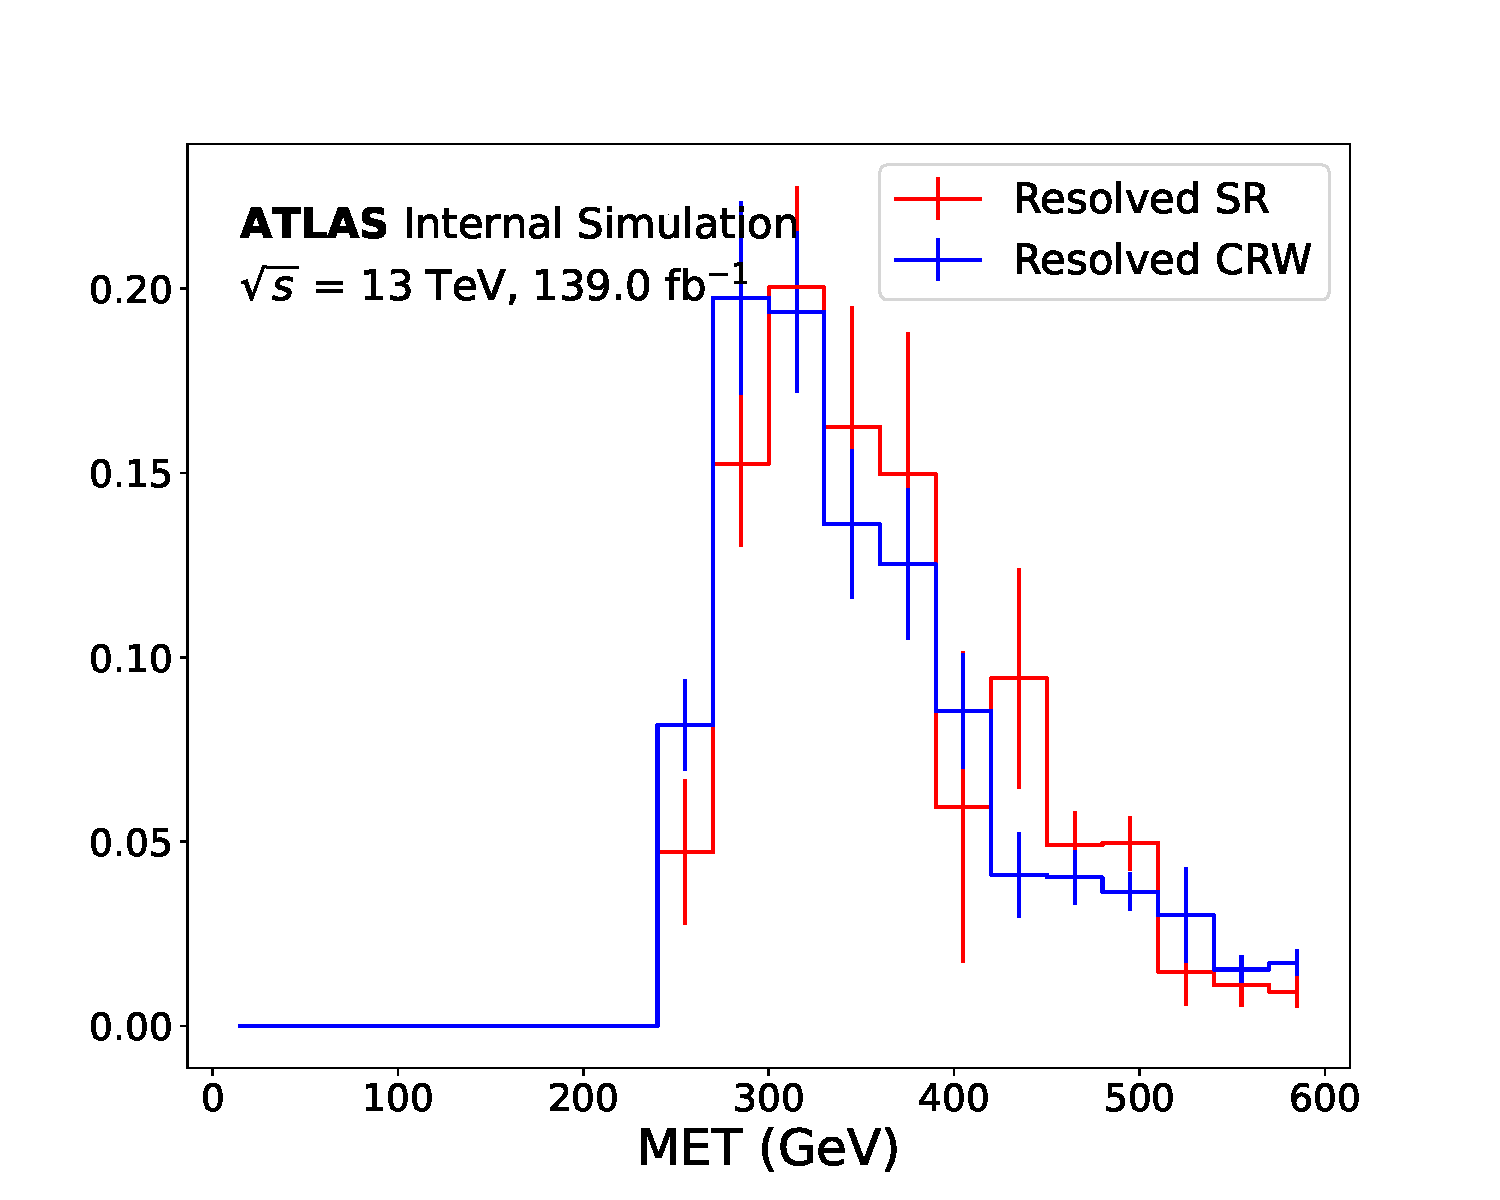
\includegraphics[width=0.5\textwidth]{Figures/5/Wjets_shapeComparison_SR_CRW.pdf}
%   \caption[\met in SR vs. CRW]{Shape comparison of \met distributions in the SR vs. the \wjets CR. Both distributions are normalized to unit area.}
%  \label{fig:MET_SR_CRW}
%\end{figure}

Table \ref{tab:Wjets_composition_CRW} compares the yield and relative composition of the \wjets background in the SRs with the \wjets CRs. Figures ~\ref{fig:signal_composition_CRW_merged} and ~\ref{fig:signal_composition_CRW_resolved} compare the signal yield and signal/background between the SR and the \wjets CR in the merged and resolved categories, respectively. The \wjets background constitutes over 75\% of the predicted yield of SM background processes in both CRs, making it the dominant SM background process, with signal contamination below \(2.5\%\) for all signal points. Thanks to the boost in the number of MC simulated events in the CRs afforded by the reversal of the \DeltaR cut, as well as the reduced lower bound on \metsig in the merged CR, the relative statistical uncertainties of the predicted \wjets yields are reduced by factors of 2 and 1.5 in the CRW compared with the SR in the merged and resolved categories, respectively. This ensures that the normalization of the \wjets background process can be predominantly established in the \wjets CR with a reasonably low statistical uncertainty. 

The benchmark used to evaluate the maximum acceptable level of signal contamination in a given CR is as follows: if the predicted yield of the signal process is negligibly small (i.e. less than \(\sim\)half as large) compared with the statistical uncertainty associated with the predicted yield of all SM background processes in the CR, then the level of signal contamination is considered acceptably small, since the presence or absence of the signal process would not be detectable given the statistical uncertainty of the total predicted yield. In the merged \wjets CR, the predicted signal yield is at most 5.1 (from Figure \ref{fig:signal_yield_CRW_merged_CR}, which is negligibly small compared with the total background yield uncertainty of 24.5 (from the third row in Table \ref{tab:Wjets_composition_CRW}). The signal yields in the resolved CRW are similarly small compared with the statistical uncertainty of the total background yield.

\begin{table}[ht]
 \centering
 \footnotesize{
\caption[Comparison of the \wjets background yield, total background yield, and the composition of the \wjets background relative to the total background.]{\label{tab:Wjets_composition_CRW} Comparison of the \wjets background yield, total background yield, and the composition of the \wjets background relative to the total background. Uncertainties on the relative composition are obtained from the sum of squared event weights.}
\begin{tabular}{l l l l}
\toprule
\textbf{Region} & \textbf{W+jets Yield} & \textbf{Total Background Yield} & \textbf{Relative W+jets Composition}\tabularnewline
\midrule
\midrule
\textbf{Merged SR} & 24.3\(\pm\)7.2 & 40.1\(\pm\)7.3 & (60.6\(\pm\)21.1)\%  \tabularnewline
\midrule
\textbf{Resolved SR} & 243.5\(\pm\)19.6 & 339.9\(\pm\)24.0 & (71.6\(\pm\)7.7)\% \tabularnewline
\midrule
\textbf{Merged CRW} & 164.0\(\pm\)23.6 & 220.6\(\pm\)24.5 & (74.3\(\pm\)13.5)\% \tabularnewline
\midrule
\textbf{Resolved CRW} & 598.1\(\pm\)30.4 & 749.5\(\pm\)31.0 & (79.8\(\pm\)5.2)\% \tabularnewline
\bottomrule
\end{tabular}}
\end{table}

\begin{figure}[htbp]
  \centering
  \begin{subfigure}{0.45\textwidth}
    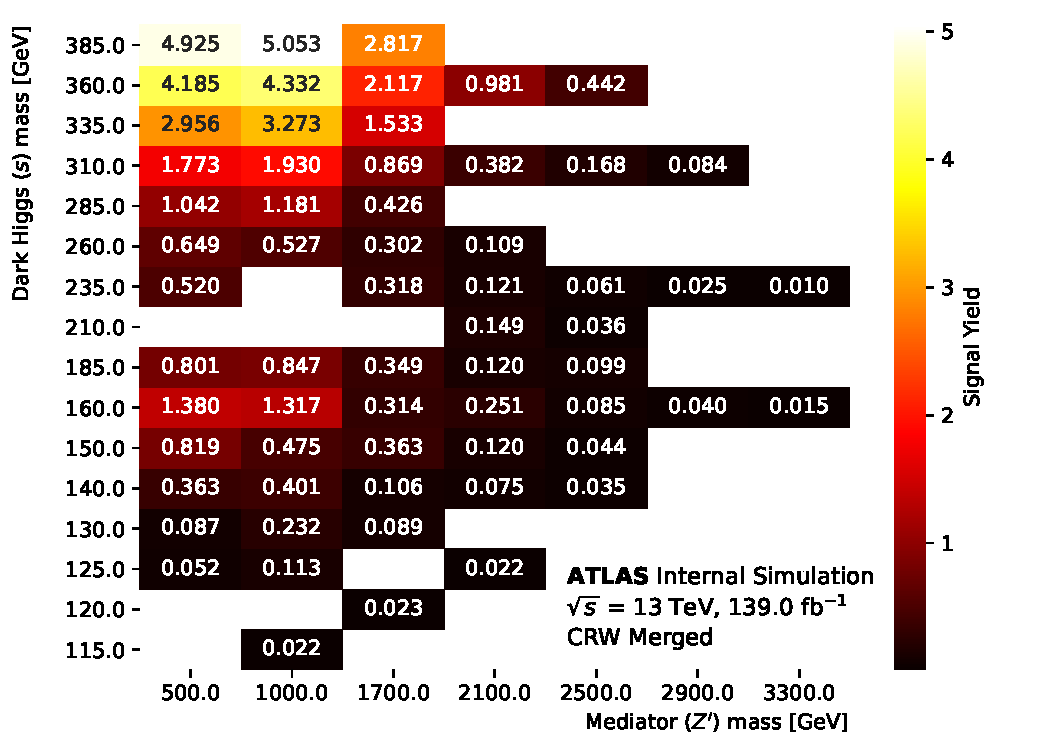
\includegraphics[width=\textwidth]{Figures/5/SignalYields_CRW_Merged.pdf}
    \caption{Signal yield in merged \wjets control region}
    \label{fig:signal_yield_CRW_merged_CR}
    \end{subfigure} \hspace{1em}
  \begin{subfigure}{0.45\textwidth}
    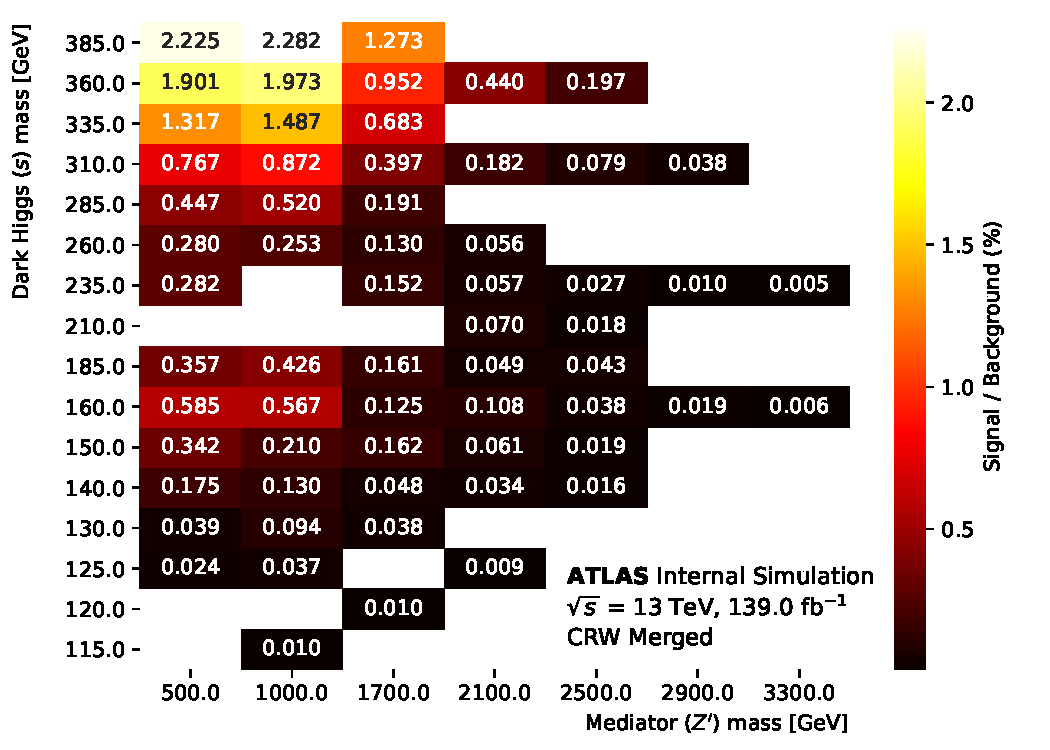
\includegraphics[width=\textwidth]{Figures/5/SignalContaminations_CRW_Merged.pdf}
    \caption{Signal / background in merged \wjets control region}
    \label{fig:signal_over_bkg_CRW_merged_CR}
    \end{subfigure}
  \caption[Predicted yields of MC simulated events for all signal points in the merged \wjets control region.]{Predicted yields of MC simulated events (left), and ratio of predicted signal / SM background yields (right) for all signal points in the merged \wjets control region.}
  \label{fig:signal_composition_CRW_merged}
\end{figure}

\begin{figure}[htbp]
  \centering
  \begin{subfigure}{0.45\textwidth}
    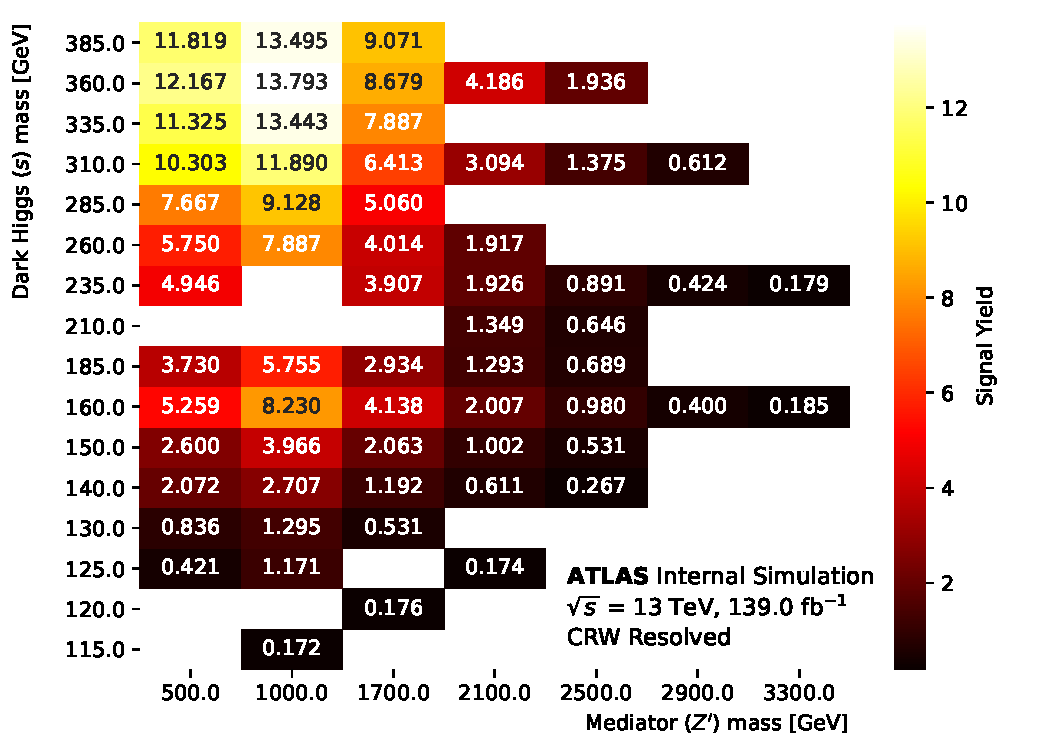
\includegraphics[width=\textwidth]{Figures/5/SignalYields_CRW_Resolved.pdf}
    \caption{Signal yield in resolved \wjets control region}\label{fig:signal_yield_CRW_resolved_CR}
    \end{subfigure} \hspace{1em}
  \begin{subfigure}{0.45\textwidth}
    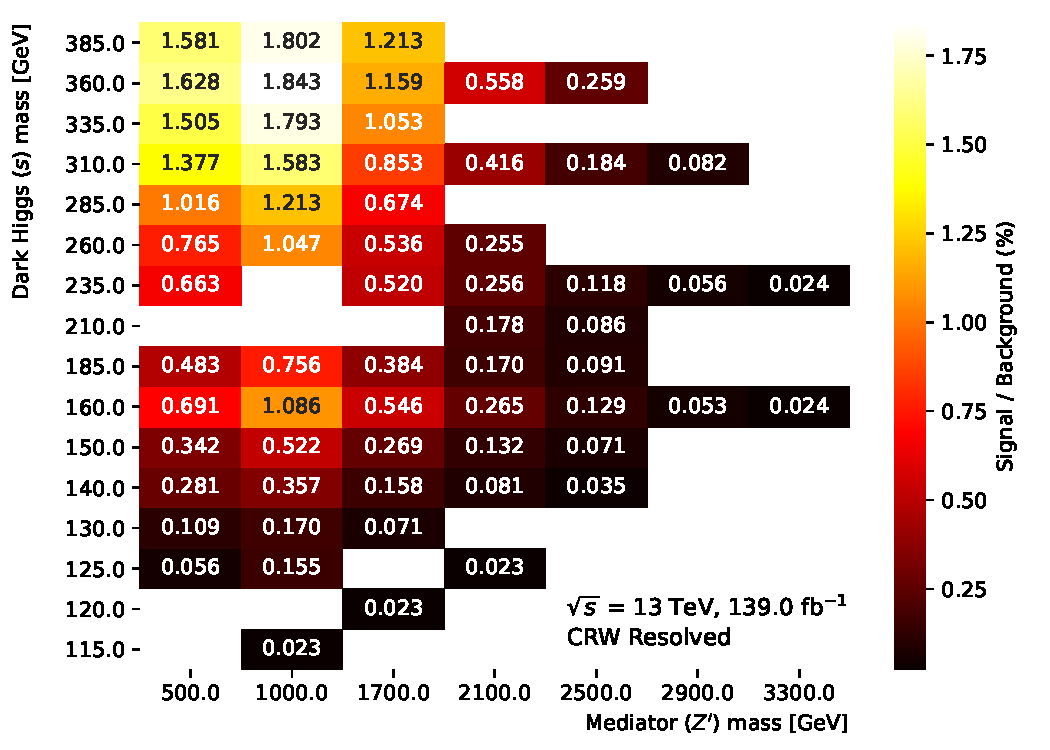
\includegraphics[width=\textwidth]{Figures/5/SignalContaminations_CRW_Resolved.pdf}
    \caption{Signal / background in resolved \wjets control region}\label{fig:signal_over_bkg_CRW_resolved_CR}
    \end{subfigure}
  \caption[Predicted yields of MC simulated events for all signal points in the resolved \wjets control region.]{Predicted yields of MC simulated events (left), and ratio of predicted signal / SM background yields (right) for all signal points in the resolved \wjets control region.}
  \label{fig:signal_composition_CRW_resolved}
\end{figure}


\subsubsection{\ttbar Control Region Definition}
\label{sec:ttbar_CR_defn}

Given that \btagged jets are vetoed in the SR to reduce the yield of events produced by the \ttbar process, a reversal of this veto presents a straightforward opportunity to define an orthogonal CR enriched with \ttbar events. Early studies found that while a simple reversal of the \bjet veto in the SR selection to instead require at least one \btagged jet was sufficient to obtain a \ttbar-enriched region with a substantially larger sample of simulated \ttbar events compared with the SR, the contamination of signal events in the region was found to be too high for a control region. 

Further tightening the \bjet veto reversal to require to at least two \btagged jets was found to reduce the signal contamination in this \ttbar CR to a reasonable level on the basis of the benchmark requirement of negligible signal yield compared with the statistical uncertainty of the total background yield discussed above in the context of the \wjets CR. However, due to the associated reduction in the number of MC simulated \ttbar events that pass this tightened requirement, it was deemed necessary to reduce the lower bound on \(\metsig\) in the merged \ttbar CR to \(\metsig>12\), as is done in the merged \wjets CR, in order to increase the number of simulated events admitted for the \ttbar process. 

 \Tab{\ref{tab:tt_CR}} summarizes the modifications made to the SR selections to define the \ttbar CR in both the merged and resolved categories. 
 
Table \ref{tab:ttbar_cr_yields} compares the yield and relative composition of the \ttbar background in the SRs with those in the \ttbar CRs. Figures ~\ref{fig:signal_composition_CRTT_merged} and ~\ref{fig:signal_composition_CRTT_resolved} compare the signal yield and signal/background between the SR and the \ttbar CR in the merged and resolved categories, respectively. As expected, the reversal of the \ttbar veto produces a region that is highly enriched in \ttbar events, which constitute \(~90\%\) of the predicted yield in the \ttbar CR. The merged and resolved \ttbar CRs admit comparable yields of \(\sim 65-70\) \ttbar events, which in both categories constitutes a several-fold increase the predicted yield compared with SR. Comparing the predicted signal yields in the merged and resolved CRTT, shown in Figures \ref{fig:signal_yield_CRTT_merged_CR} and \ref{fig:signal_yield_CRTT_resolved_CR} respectively, with the statistical uncertainties associated with the total yield of events in these CRTTs from Table \ref{tab:tt_CR}, the predicted signal yields are in all cases well below the statistical uncertainty of the background yield, and thus constitute a reasonably low level of signal contamination the CRTT.


\begin{table}[ht]
 \centering
\caption[Summary of differences in selections on \(N(\bjet)\) and \metsig between signal regions and \ttbar control regions.]{\label{tab:tt_CR} Summary of differences in selections on \(N(\bjet)\) and \metsig between signal regions and \ttbar control regions.}
\begin{tabular}{l l l}
\toprule
\textbf{Region} & \textbf{\btagged Jet Veto/Requirement} & \textbf{\metsig Cut} \tabularnewline
\midrule
\midrule
\textbf{Merged SR} & \(N(\bjet) = 0\) & \(\metsig > 16\)\tabularnewline
\midrule
\textbf{Resolved SR} & \(N(\bjet) = 0\) & \(\metsig > 16\)\tabularnewline
\midrule
\textbf{Merged CRTT} & \(N(\bjet) > 1\) & \(\metsig > 12\)\tabularnewline
\midrule
\textbf{Resolved CRTT} & \(N(\bjet) > 1\) & \(\metsig > 16\)\tabularnewline
\bottomrule
\end{tabular}
\end{table}

\begin{figure}[htbp]
  \centering
  \begin{subfigure}{0.45\textwidth}
    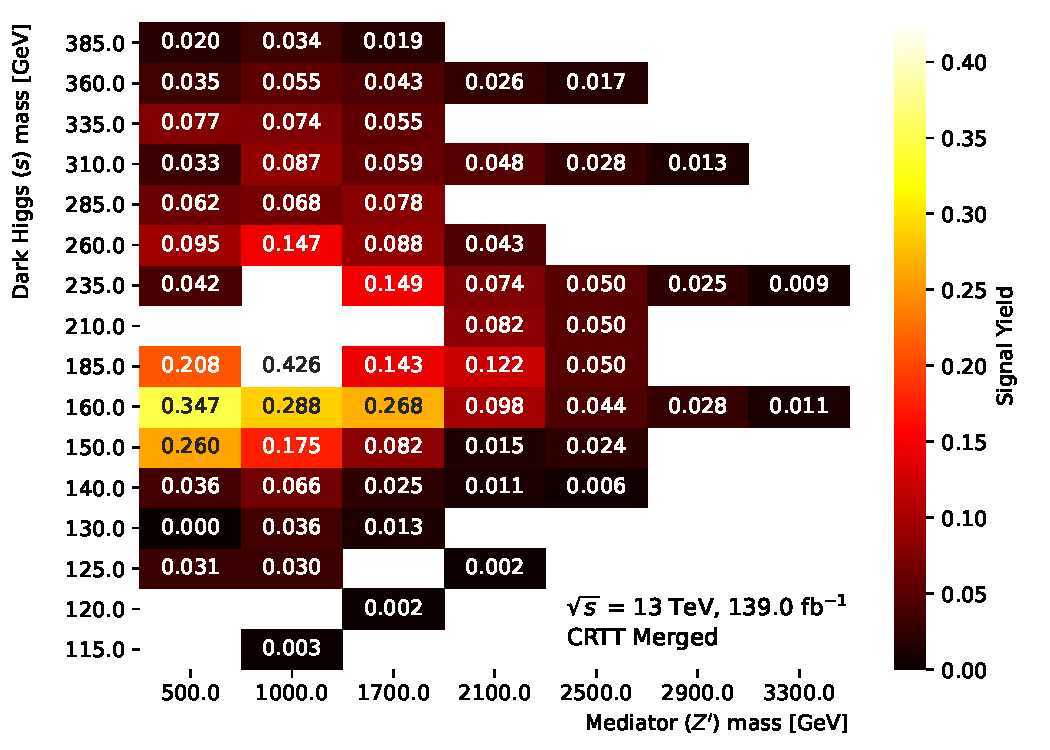
\includegraphics[width=\textwidth]{Figures/5/SignalYields_CRTT_Merged.pdf}
    \caption{Signal yield in merged \ttbar control region}
    \label{fig:signal_yield_CRTT_merged_CR}
    \end{subfigure} \hspace{1em}
  \begin{subfigure}{0.45\textwidth}
    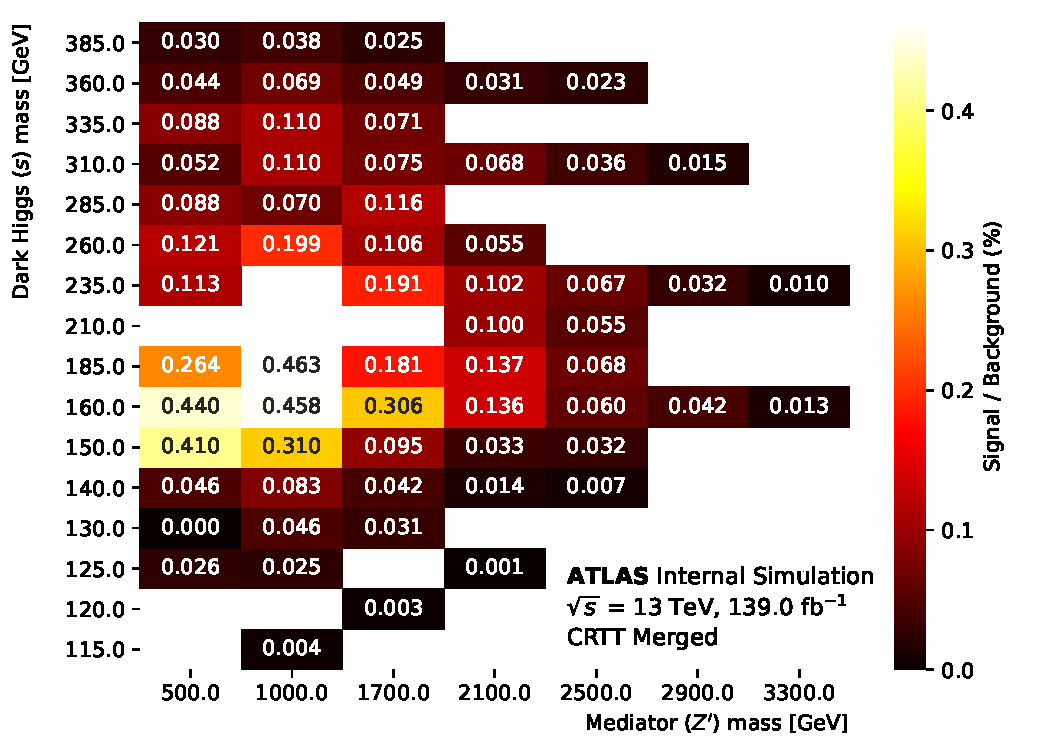
\includegraphics[width=\textwidth]{Figures/5/SignalContaminations_CRTT_Merged.pdf}
    \caption{Signal / background in merged \ttbar enriched control region}
    \label{fig:signal_over_bkg_CRTT_merged_CR}
    \end{subfigure}
  \caption[Predicted yields of MC simulated events for all signal points in the merged \ttbar control region.]{Predicted yields of MC simulated events (left), and ratio of predicted signal / SM background yields (right) for all signal points in the merged \ttbar control region.}
  \label{fig:signal_composition_CRTT_merged}
\end{figure}

\begin{figure}[htbp]
  \centering
  \begin{subfigure}{0.45\textwidth}
    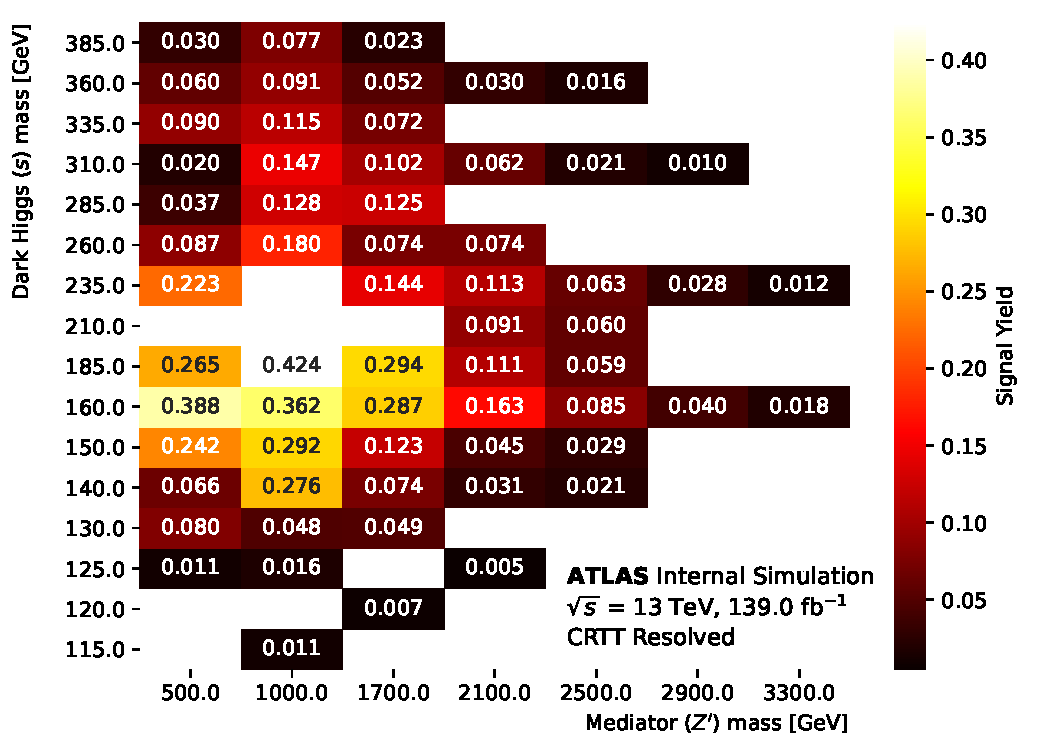
\includegraphics[width=\textwidth]{Figures/5/SignalYields_CRTT_Resolved.pdf}
    \caption{Signal yield in resolved \ttbar control region}
    \label{fig:signal_yield_CRTT_resolved_CR}
    \end{subfigure} \hspace{1em}
  \begin{subfigure}{0.45\textwidth}
    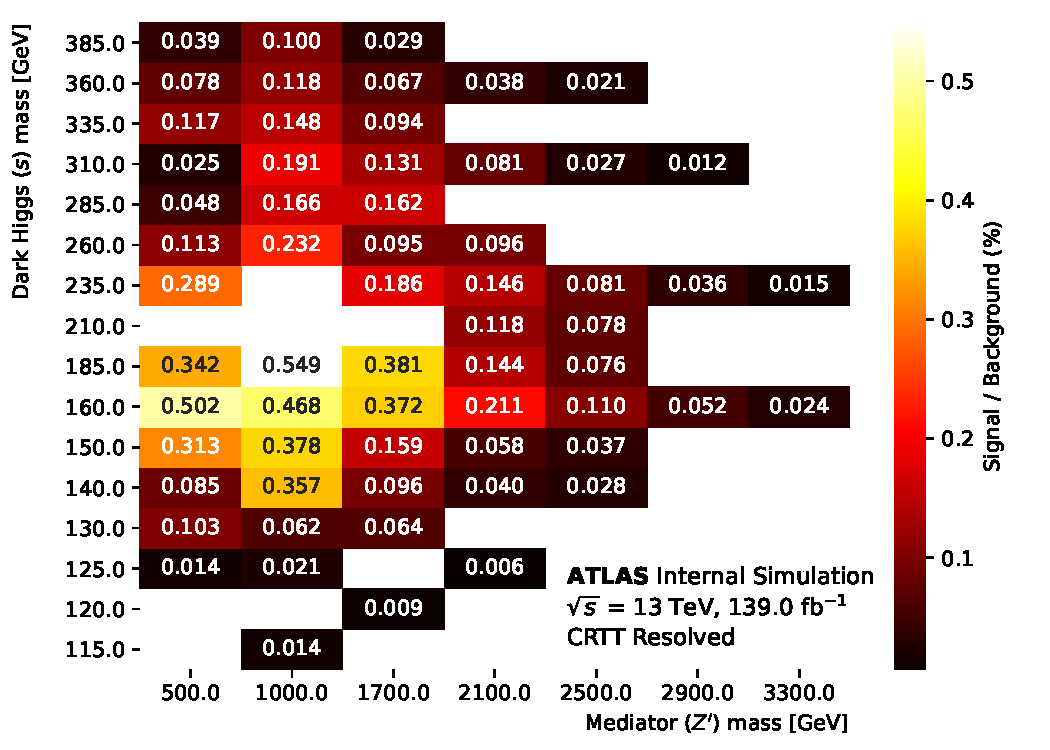
\includegraphics[width=\textwidth]{Figures/5/SignalContaminations_CRTT_Resolved.pdf}
    \caption{Signal / background in resolved \ttbar enriched control region}
    \label{fig:signal_over_bkg_CRTT_resolved_CR}
    \end{subfigure}
  \caption[Predicted yields of MC simulated events for all signal points in the resolved \ttbar control region.]{Predicted yields of MC simulated events (left), and ratio of predicted signal / SM background yields (right) for all signal points in the resolved \ttbar control region.}
  \label{fig:signal_composition_CRTT_resolved}
\end{figure}

\begin{table}[htbp]
    \centering
    \caption[Comparison of the \ttbar background yield, total background yield, and the composition of the \ttbar background relative to the total background.]{Comparison of the \ttbar background yield, total background yield, and the composition of the \ttbar background relative to the total background. Uncertainties on the relative composition are obtained from the sum of squared event weights.}
    \begin{tabular}{l l l l}
      \toprule
     \textbf{Region} & \(\boldsymbol{t\bar{t}}\)\textbf{ Yield} & \textbf{Total Background Yield} & \(\boldsymbol{t\bar{t}}\)\textbf{ Relative Composition} \\
      \midrule
      \midrule
      \textbf{Merged SR} & 4.3\(\pm\)0.3 & 40.1\(\pm\)7.3 & (10.7\(\pm\)2.1)\%  \tabularnewline
      \midrule
      \textbf{Resolved SR} & 21.2\(\pm\)0.7 & 339.9\(\pm\)24.0 & (6.2\(\pm\)0.5)\% \tabularnewline
      \midrule
      \textbf{Merged CRTT} & 70.5\(\pm\)1.7 & 74.8\(\pm\)5.0 & (94.2\(\pm\)6.7)\% \tabularnewline
      \midrule
      \textbf{Resolved CRTT} & 64.2\(\pm\)1.2 & 73.3\(\pm\)4.9 & (83.1\(\pm\)3.4)\% \tabularnewline
      \bottomrule
    \end{tabular}
    \label{tab:ttbar_cr_yields}
\end{table}

Kinematic distributions of interest are compared between the \ttbar CRs and the SRs in Figures \ref{fig:N_1_CRTT_merged} and \ref{fig:N_1_CRTT_resolved} in Appendix \ref{app:appendix_SR_CR_distributions_ttbar}. A similar bias towards lower \met that was discussed in the context of the merged \wjets CR is also seen in the merged CRTT, and is similarly attributable to the loosened lower bound on \(\metsig\) in this region. The level of shape agreement in the other distributions is considered to be close enough to conclude that events in the \ttbar CR occupy a sufficiently similar region of kinematic phase space as events in the SR to justify applying data-driven \ttbar normalization constraints obtained in this CR to the SR.

\subsection{Background Yields}
\label{ap:bkg_yields}

Tables \ref{tab:bkg_yield_merged} and \ref{tab:bkg_yield_resolved} show the overall background yields in the merged and resolved analysis regions, respectively, after application of all the analysis selections described in this section.

\begin{table}[ht]
\centering
\caption[Background yields after application of all analysis cuts in the merged analysis regions.]{\label{tab:bkg_yield_merged} Background yields after application of all analysis cuts in the merged analysis regions. Uncertainty on the yields is statistical.}
\begin{tabular}{l l l l}
\toprule
\textbf{Background} & \textbf{Merged SR} & \textbf{Merged CRW} & \textbf{Merged CRTT}\tabularnewline
\midrule
\midrule
\textbf{W+jets} & 24.2 \(\pm\) 7.2 & 164.0 \(\pm\) 23.6 & -1.3 \(\pm\) 4.6\tabularnewline
\midrule
\(\mathbf{\ttbar}\) & 4.3 \(\pm\) 0.3 & 9.9 \(\pm\) 0.6 & 70.4 \(\pm\) 1.6\tabularnewline
\midrule
\textbf{Diboson} & 7.6 \(\pm\) 0.3 & 26.8 \(\pm\) 1.5 & 0.2 \(\pm\) 0.0\tabularnewline
\midrule
\textbf{Triboson} & 1.2 \(\pm\) 0.1 & 1.9 \(\pm\) 0.1 & 0.0 \(\pm\) 0.0\tabularnewline
\midrule
\textbf{Z+jets} & 1.1 \(\pm\) 0.9 & 15.2 \(\pm\) 6.3 & 0.0 \(\pm\) 0.0\tabularnewline
\midrule
\textbf{single \(t\)} & 1.6 \(\pm\) 0.5 & 2.7 \(\pm\) 0.6 & 5.4 \(\pm\) 0.9\tabularnewline
\midrule
\textbf{Total} & 40.1 \(\pm\) 7.3 & 220.6 \(\pm\) 24.5 &74.8 \(\pm\) 5.0\tabularnewline
\bottomrule
\end{tabular}
\end{table}

\begin{table}[ht]
\centering
\caption[Background yields after application of all analysis cuts in the resolved analysis regions.]{\label{tab:bkg_yield_resolved} Background yields after application of all analysis cuts in the resolved analysis regions. Uncertainty on the yields is statistical.}
\begin{tabular}{l l l l}
\toprule
\textbf{Background} & \textbf{Resolved SR} & \textbf{Resolved CRW} & \textbf{Resolved CRTT}\tabularnewline
\midrule
\midrule
\textbf{W+jets} & 243.5 \(\pm\) 19.6 & 598.1 \(\pm\) 30.4 & 1.5 \(\pm\) 2.2\tabularnewline
\midrule
\(\mathbf{\ttbar}\) & 21.2 \(\pm\) 0.7 & 20.0 \(\pm\) 0.7 & 64.2 \(\pm\) 1.2\tabularnewline
\midrule
\textbf{Diboson} & 51.1 \(\pm\) 1.1 & 105.5 \(\pm\) 1.5 & 0.6 \(\pm\) 0.0\tabularnewline
\midrule
\textbf{Triboson} & 3.0 \(\pm\) 0.2 & 5.6 \(\pm\) 0.3 & 0.0 \(\pm\) 0.0\tabularnewline
\midrule
\textbf{Z+jets} & 17.4 \(\pm\) 13.7 & 17.1 \(\pm\) 6.0 & 0.0 \(\pm\) 0.0\tabularnewline
\midrule
\textbf{single \(t\)} & 3.7 \(\pm\) 0.8 & 3.2 \(\pm\) 0.7 & 11.0 \(\pm\) 1.2\tabularnewline
\midrule
\textbf{Total} & 339.9 \(\pm\) 24.0 &749.5 \(\pm\) 31.0 &77.3 \(\pm\) 2.8\tabularnewline
\bottomrule
\end{tabular}
\end{table}

\section{Triggers}
\label{sec:triggers_evt_selection}

As discussed in Section \ref{sec:trigger}, the ATLAS trigger system only saves collision events that pass both the hardware-based level-1 (L1) trigger and the software-based high-level trigger (HLT). The L1 trigger and the HLT are each comprised of numerous sets of selection criteria, which are also referred to as triggers. Any collision event that satisfies at least one of the triggers that comprise the L1 trigger is processed by the HLT. Likewise, if the event satisfies any of the triggers that comprise the HLT, it will be saved for later analysis.

The search presented in this thesis is interested in events that produce a single energetic lepton due to the \(s\rightarrow WW(q\bar{q}\ell\nu)\) decay, in addition to high \met due both to the undetected boosted DM in the final state, and to the undetected \(\nu\) from the \(W\rightarrow \ell\nu\) decay. It is important to determine the efficiency with which the ATLAS trigger system accepts events in the region of phase space defined by the event selections described in Section \ref{sec:evt_selections} above. This efficiency quantifies the probability that an event that the triggers are designed to accept successfully passes the trigger criteria and gets accepted. If the trigger efficiency is \(<100\%\) in any area of the phase space considered in the analysis, it is in general necessary to apply scale factors to any MC simulated events that fall into this phase space to account for the fact that some of these events would have been rejected by the trigger during actual data-taking. It is also then necessary to evaluate and propagate uncertainties associated with these scale factors.

To simplify the trigger efficiency analysis and determine whether any scale factors may be needed, it is helpful to identify a minimal list of triggers that all events considered in the analysis would be expected to pass. One of the event selection criteria for the analysis, presented in Section \ref{sec:evt_selections}, requires all events to have \(\met > 200~\GeV\). Since the ATLAS \met trigger, described in Refs. \cite{met_trigger_performance_2020} and \cite{met_performance_2019}, is designed to efficiently select events with \(\met>150~\GeV\), it is reasonable to expect events that pass the event selection criteria to have also passed the \met trigger with a high efficiency. The specific \met triggers in the ATLAS trigger menu that are considered in this study are chosen following ATLAS recommendations, and vary between different data collection periods defined by ATLAS. The full list of \met triggers used, along with the associated data collection period for each, is listed in Table \ref{tab:summary_triggers_used}.

\begin{table}[ht]
\caption[Summary of \met triggers from the ATLAS trigger menu used for the search.]{Summary of \met triggers from the ATLAS trigger menu used for the search, along with the associated data collection period for each trigger.}
\label{tab:summary_triggers_used}
\footnotesize{
	\begin{center}
	\begin{tabular}{l l }
		\toprule
			\textbf{Period} & \textbf{MET Trigger} \\
			\midrule
			\midrule
			2015 & \textsc{HLT\_xe70\_mht} \\
			\midrule
			2016 (A-D3) & \textsc{HLT\_xe90\_mht\_L1XE50} \\
			\midrule
			2016 (D4-F1) & \textsc{HLT\_xe100\_mht\_L1XE50} \\
			\midrule
			2016 (F2-) & \textsc{HLT\_xe110\_mht\_L1XE50} \\
			\midrule
			2017 (B-D5) & \textsc{HLT\_xe110\_pufit\_L1XE55} \\
			\midrule
			2017 (D6-K) & \textsc{HLT\_xe110\_pufit\_L1XE50} \\
			\midrule
			2018 (B-C5) & \textsc{HLT\_xe110\_pufit\_xe70\_L1XE50} \\
			\midrule
			2018 (C5-) & \textsc{HLT\_xe110\_pufit\_xe65\_L1XE50} \\
		\bottomrule
	\end{tabular}
	\end{center}
	}
\end{table}

The ATLAS trigger system also includes single-muon and single-electron triggers, which are designed to pass events in which a single muon (electron) is reconstructed in the final state and satisfies some minimum \pt requirement. Since all events considered in the search are required to have a single lepton in the final state, events which pass the event selection would also be expected to pass these charged lepton triggers with high efficiency. The specific single muon and electron triggers considered in this study, along with the ATLAS data-taking period(s) in which they were applied and the minimum lepton \pt requirement associated with each trigger, are listed in Tables \ref{tab:summary_muon_triggers_used} and \ref{tab:summary_electron_triggers_used}, respectively.

\begin{table}[ht]
\caption[Summary of single muon triggers from the ATLAS trigger menu used for the search.]{Summary of single muon triggers from the ATLAS trigger menu used for the search, along with the associated data collection period for each trigger. The minimum muon \pt threshold of each trigger is also listed.}
\label{tab:summary_muon_triggers_used}
\footnotesize{
	\begin{center}
	\begin{tabular}{l l l }
		\toprule
			\textbf{Periods} & \textbf{Single Muon Trigger} & \textbf{Muon \pt threshold} \\
			\midrule
			\midrule
			2015 & \textsc{HLT\_mu20\_iloose\_L1MU15} & 20 \GeV \\
			\midrule
			2016 (A, B-D3, D4-E, F-G2, G3-I3, I4-), & \multirow{3}{*}{\textsc{HLT\_mu50}} & \multirow{3}{*}{50 \GeV} \\
			2017 (B-), & & \\
			2018 & & \\
			\midrule
			2016 & \textsc{HLT\_mu24\_iloose} & 24 \GeV \\
			\midrule
			2015, & \multirow{2}{*}{\textsc{HLT\_mu40}} & \multirow{2}{*}{40 \GeV} \\
			2016 (A) & & \\
			\midrule
			2016 (B-D3, D4-E) & \textsc{HLT\_mu24\_ivarmedium} & 24 \GeV \\
			\midrule
			2016 (D4-E, F-G2, G3-I3, I4-),  & \multirow{3}{*}{\textsc{HLT\_mu26\_ivarmedium}} & \multirow{3}{*}{26 \GeV} \\
			2017 (B-), \\
			2018 \\
		\bottomrule
	\end{tabular}
	\end{center}
	}
\end{table}

\begin{table}[ht]
\caption[Summary of single electron triggers from the ATLAS trigger menu used for the study presented in Section \ref{sec:triggers_evt_selection}.]{Summary of single electron triggers from the ATLAS trigger menu used for the study presented in Section \ref{sec:triggers_evt_selection}, along with the associated data collection period for each trigger. The minimum electron \pt threshold of each trigger is also listed.}
\label{tab:summary_electron_triggers_used}
\footnotesize{
	\begin{center}
	\begin{tabular}{l l l }
		\toprule
			\textbf{Periods} & \textbf{Single Muon Trigger} & \textbf{Electron \pt threshold} \\
			\midrule
			\midrule
			2015 & \textsc{HLT\_e24\_lhmedium\_L1EM20VH} & 24 \GeV \\
			\midrule
			2015 & \textsc{HLT\_e60\_lhmedium} & 60 \GeV \\
			\midrule
			2015 & \textsc{HLT\_e120\_lhloose} & 120 \GeV \\
			\midrule
			2016 (A, B-D3) & \textsc{HLT\_e24\_lhtight\_nod0\_ivarloose} & 24 \GeV \\
			\midrule
			2016 (A, B-D3, D4-F, G-), & \multirow{3}{*}{\textsc{HLT\_e60\_lhmedium\_nod0}} & \multirow{3}{*}{60 \GeV} \\
			2017 (B-), & & \\
			2018 & & \\
			\midrule
			2016 (A, B-D3, D4-F, G-)  & \textsc{HLT\_e60\_medium} & 60 \GeV \\
			\midrule
			2016 (A, B-D3, D4-F, G-),  & \multirow{3}{*}{\textsc{HLT\_e300\_etcut}} & \multirow{3}{*}{300 \GeV} \\
			2017 (B-), & & \\
			2018 \\
			\midrule
			2016 (A, B-D3, D4-F, G-), & \multirow{3}{*}{\textsc{HLT\_e140\_lhloose\_nod0}} & \multirow{3}{*}{140 \GeV} \\
			2017 (B-), & & \\
			2018 & & \\
			\midrule
			2016 (D4-F, G-), & \multirow{3}{*}{\textsc{HLT\_e26\_lhtight\_nod0\_ivarloose}} & \multirow{3}{*}{26 \GeV} \\
			2017 (B-) & & \\
			2018 & & \\
		\bottomrule
	\end{tabular}
	\end{center}
	}
\end{table}

The lepton triggers are known to be \(<100\%\) efficient, but the resulting scale factors and associated systematic uncertainties are in general well calibrated by dedicated measurements performed within the ATLAS collaboration. As a result, the charged lepton triggers are useful as a means of independently quantifying the efficiency of the \met trigger, as will be shown in a moment. However, if the \met trigger can be shown to pass the events considered in this search with 100\% efficiency then there is no need to apply scaling factors or evaluate related uncertainties.
%it is desirable simply to explicitly require all selected events to have additionally passed the \met trigger in order to avoid any need to apply scaling factors and evaluate related uncertainties.

The efficiency of the \met trigger for a set of event selection criteria that define a given region ``X" is defined equivalently for ATLAS data (``data") and MC simulated events (``MC"). Events considered for the calculation of trigger efficiency are also required to have passed the single lepton trigger (defined as the logical OR of the single muon trigger and the single electron trigger), to independently ensure that all data events considered passed a trigger that is relevant to the final state of interest. The trigger efficiency is given by:

\begin{equation}
\label{eq:met_trig_eff}
\begin{footnotesize}
\text{eff}_\text{\met, region X} = \frac{\sum_i w_i\text{ passing (\met triggers)\&(single lepton triggers)\&(selection cuts for region X)}}{\sum_i w_i\text{ passing (single lepton triggers)\text{ AND }(selection cuts for region X)}}
\end{footnotesize}
\end{equation}

\noindent where $w_i$ is the total event weight for event \(i\) ($w_i=1$ in the case of data). See Section \ref{sec:evt_wts} for a detailed discussion of weights that are assigned to the MC simulated events. Correction scale factors, dependent on the \pt and \(\eta\) of the final-state lepton in each event, are included in the MC event weights in Eq. \ref{eq:met_trig_eff} to account for the \(<100\%\) trigger efficiency of the single lepton triggers. 

Figure \ref{fig:mettrig} compares the \met trigger efficiency defined in Eq. \ref{eq:met_trig_eff} for MC simulated events and ATLAS data for the region defined with the baseline selections, with the following modifications:

\begin{itemize}
\item A range of lower bounds on the \met are considered, from \(\sim100~\GeV\) to \(\sim500~\GeV\).
\item The single charged lepton is required to be an electron (a.k.a. the ``electron channel") in Figure \ref{fig:mettrig_e} and a muon (a.k.a. the ``muon channel") in Figure \ref{fig:mettrig_mu}.
\end{itemize}

\begin{figure}[htbp]
  \centering
     \begin{subfigure}{0.49\textwidth}
     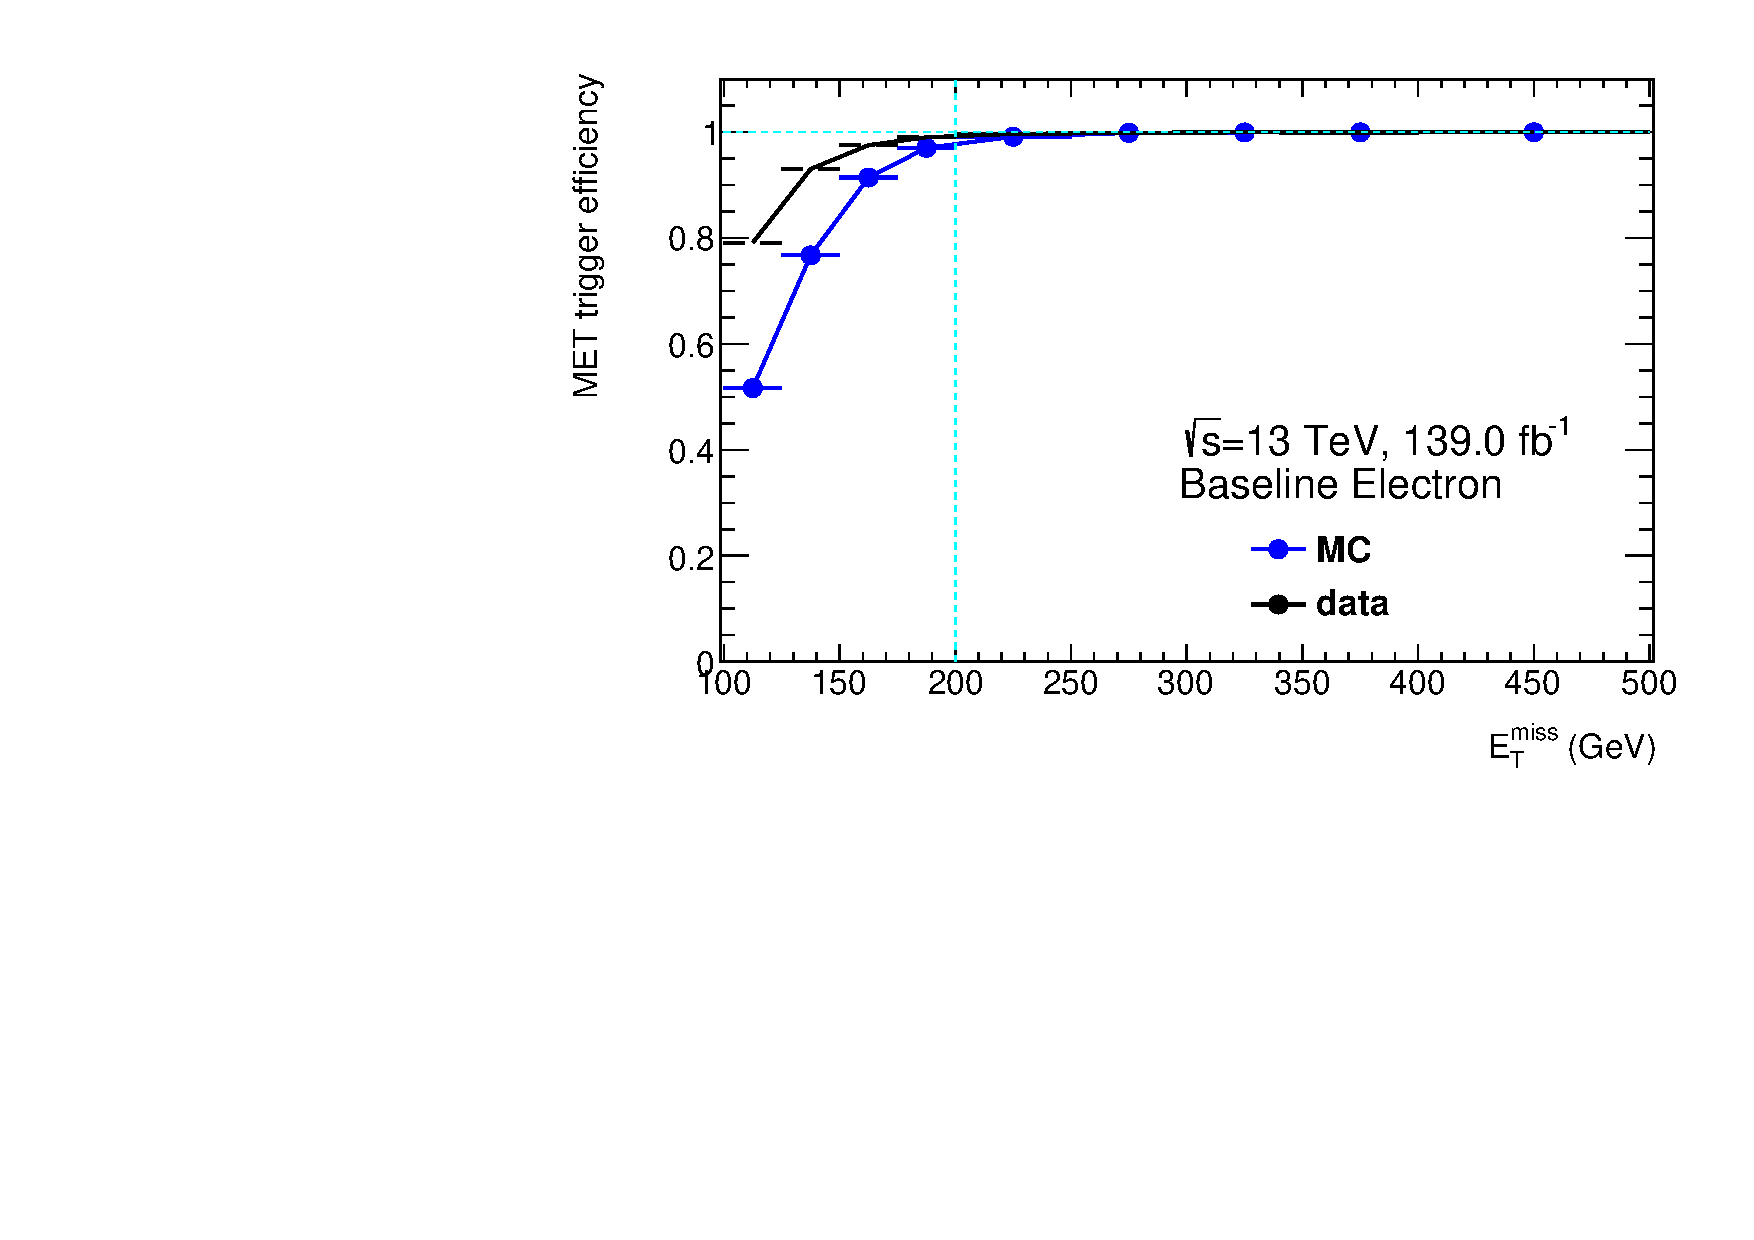
\includegraphics[width = 0.98\textwidth]{Figures/5/efficiency_baseline_electron.pdf}
    \caption{Electron Channel}
    \label{fig:mettrig_e}
     \end{subfigure}
    \begin{subfigure}{0.49\textwidth}
     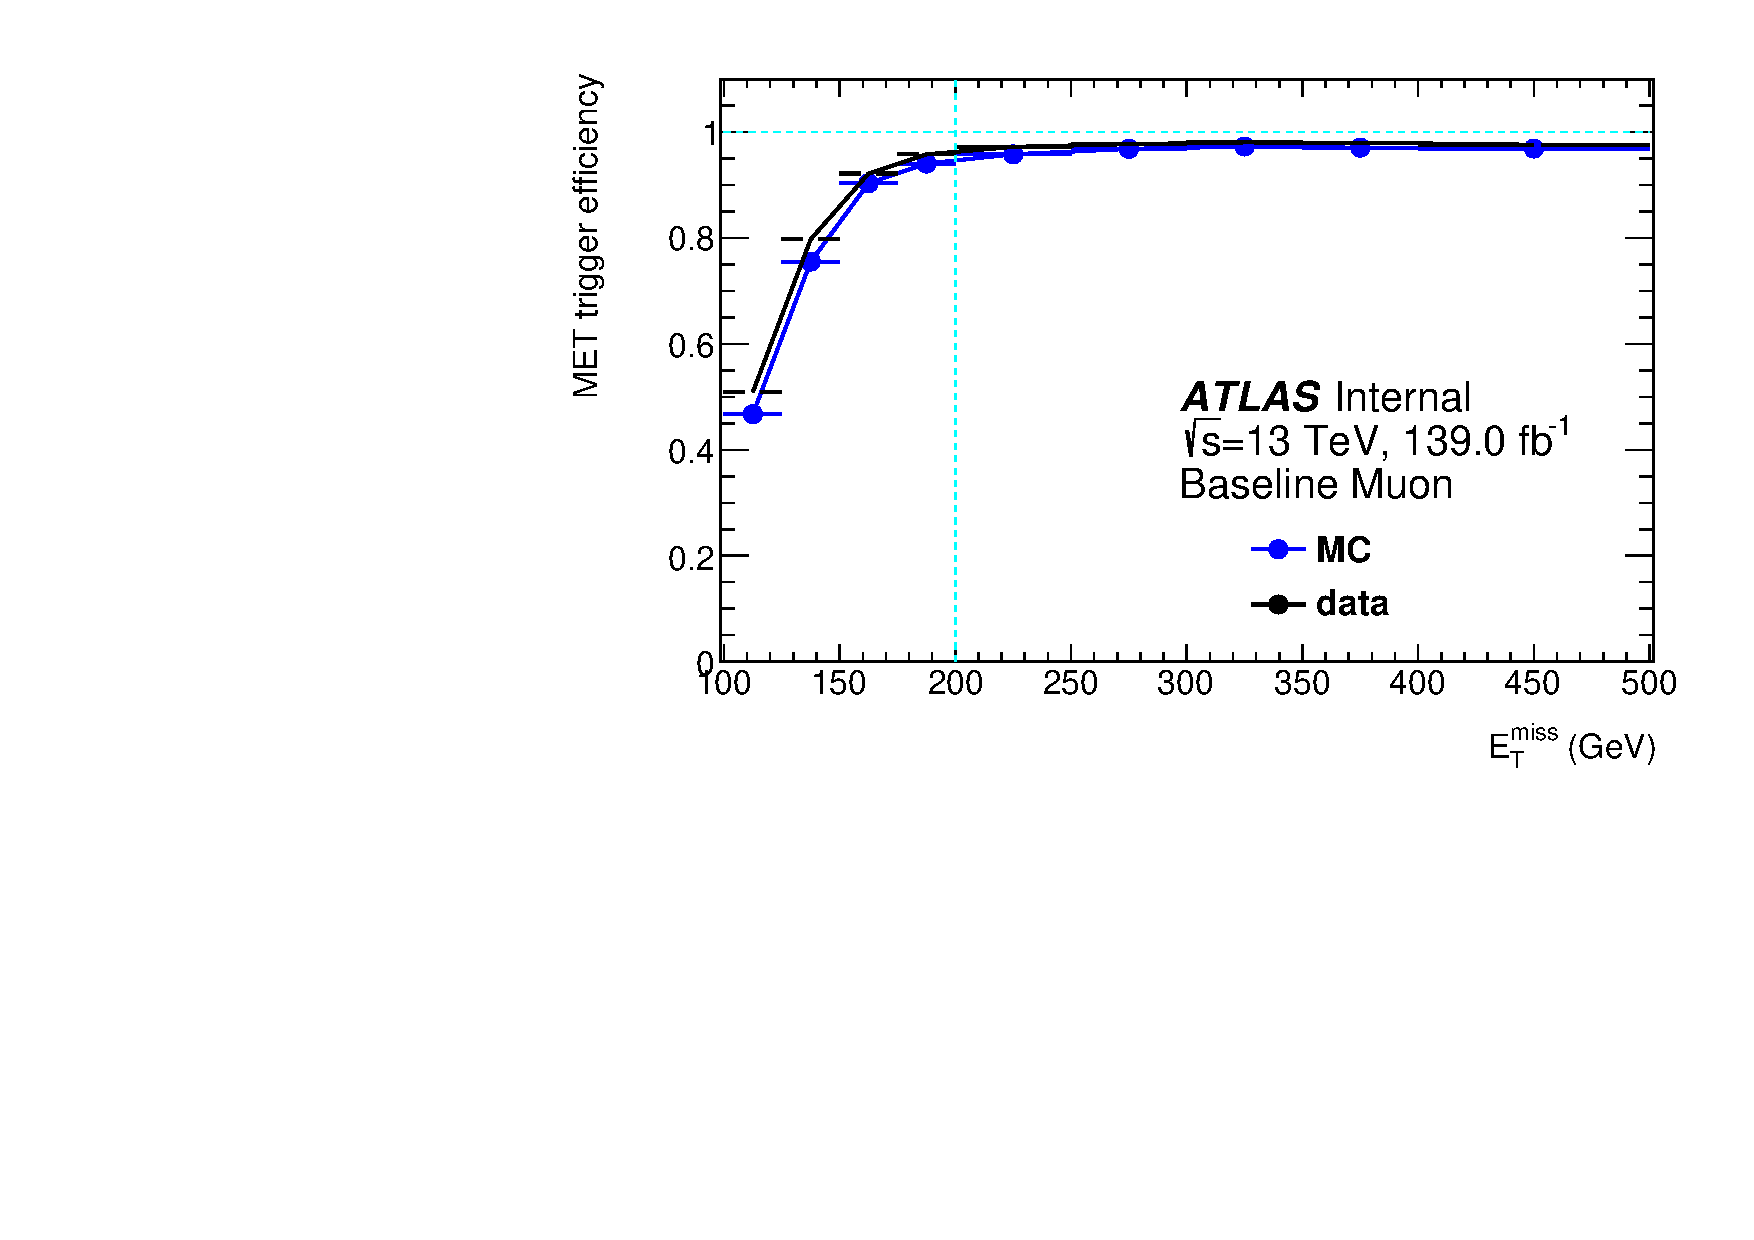
\includegraphics[width = 0.98\textwidth]{Figures/5/efficiency_baseline_muon.pdf}
     \caption{Muon Channel}
     \label{fig:mettrig_mu}
     \end{subfigure}
         \begin{subfigure}{0.49\textwidth}
     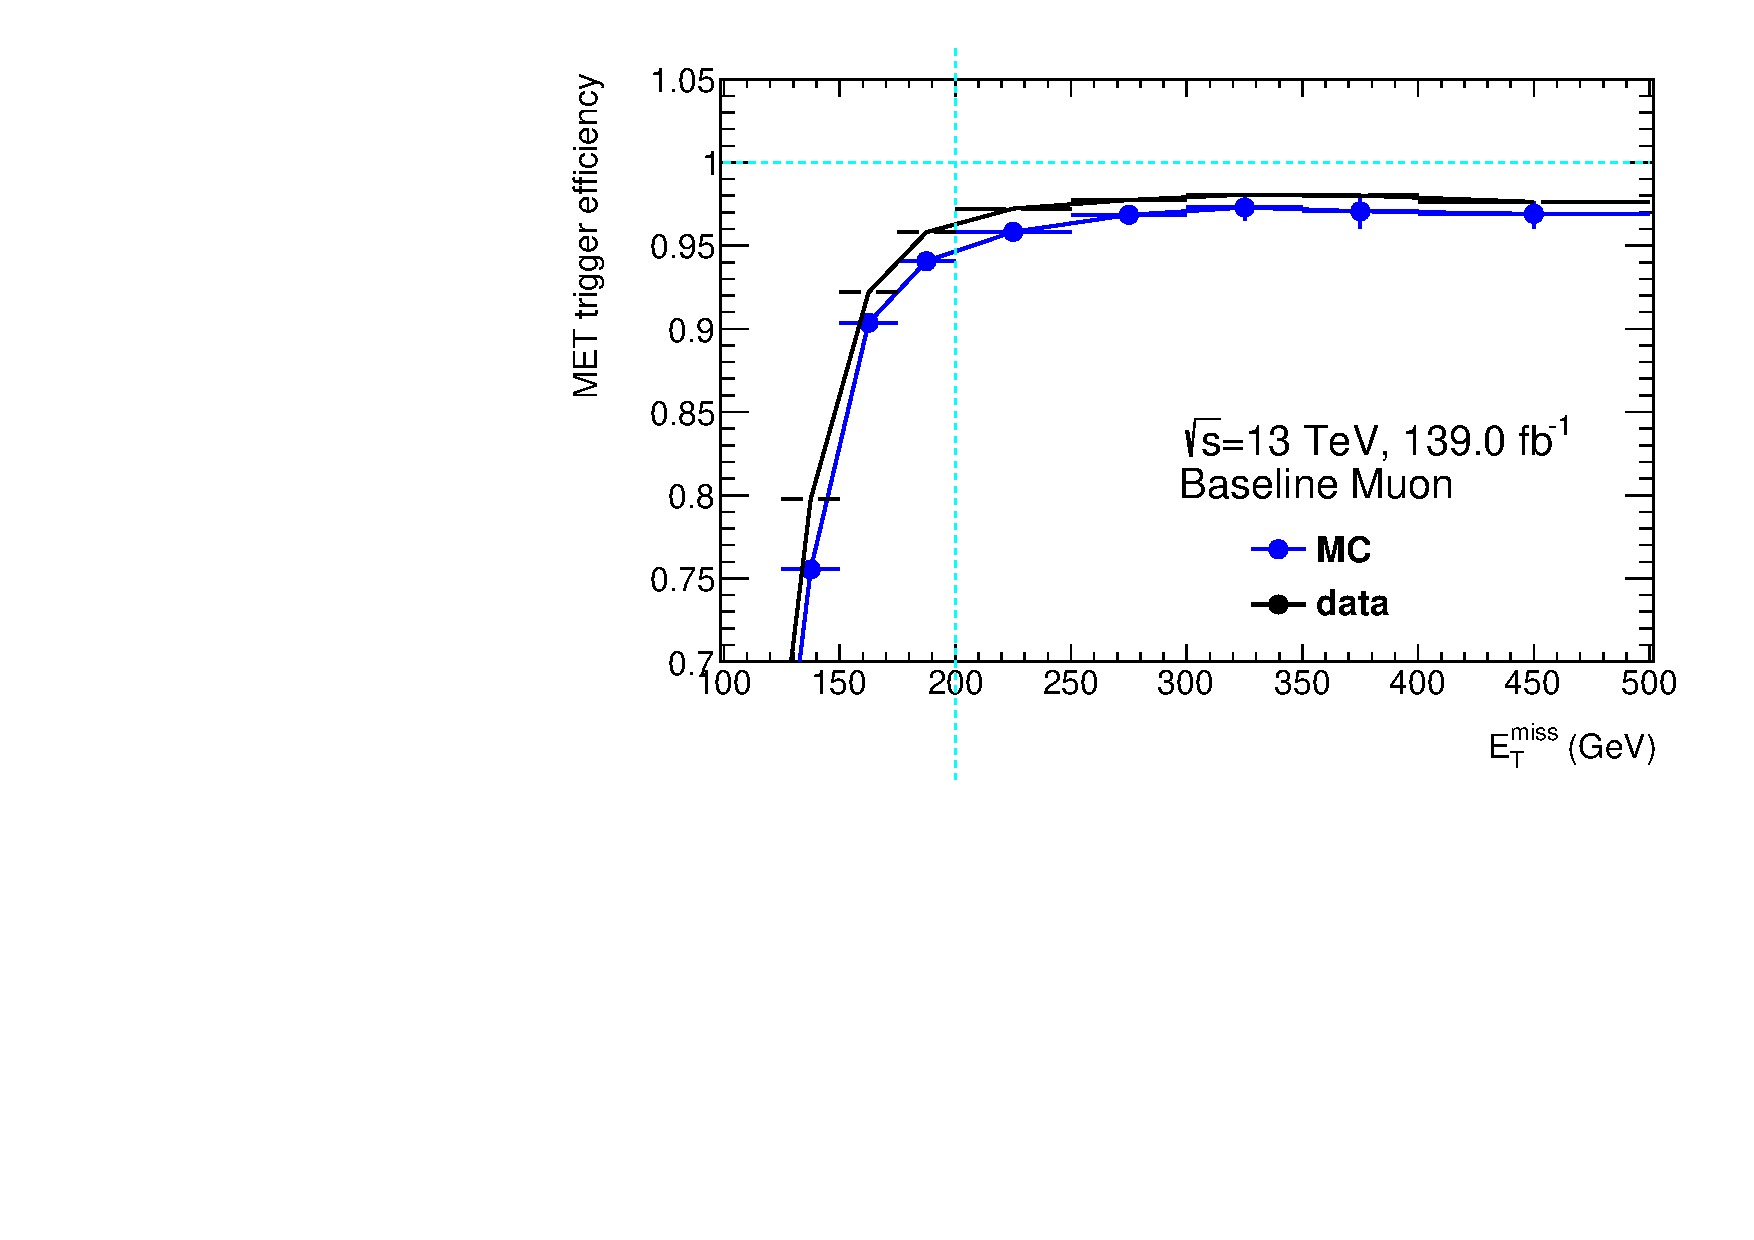
\includegraphics[width = 0.98\textwidth]{Figures/5/efficiency_baseline_muon_zoom.pdf}
     \caption{Muon Channel (y-axis range reduced)}
     \label{fig:mettrig_mu_zoom}
     \end{subfigure}
     \caption[Comparison of the \met trigger efficiency between MC simulated events and ATLAS data.]{Comparison of the \met trigger efficiency defined in Eq. \ref{eq:met_trig_eff}, as a function of the \met lower bound in the event selection, between MC simulated events and ATLAS data in a region defined by the baseline selection. The event selection is separated into electron (top left) and muon (top right and bottom center) channels.}
     \label{fig:mettrig}
  \end{figure}
  
Comparing the trigger efficiencies in the electron channel (Figure \ref{fig:mettrig_e}) and the muon channel (Figures \ref{fig:mettrig_mu} and \ref{fig:mettrig_mu_zoom}), the efficiency in the electron channel converges to 100\% for \(\met > 200~\GeV\), but in the muon channel it instead converges to \(\sim97\%\) for \(\met > 200~\GeV\). After some investigation, the inefficiency in the muon channel was found to be due to events with large \met arising from high-\pt muons. This is because high-\pt muons leave very little energy in the ATLAS calorimeter and are detected instead by the muon spectrometer. As a result, such high-\pt muon events can be missed by the \met triggers, which don't use information from the muon spectrometer (see Section 3 of Ref. \cite{met_performance_2019} for details of the construction of \met for the ATLAS \met trigger). This can be seen by plotting the \met trigger efficiency using a calculation of \met in the event selection that ignores the muon \pt (a.k.a. ``muon invisible") in Figure \ref{fig:metmuinvis}, and observing that in this case the efficiency converges to 100\% for \met (muon invisible) \(> 200~\GeV\). 

\begin{figure}[htbp]
    \centering
     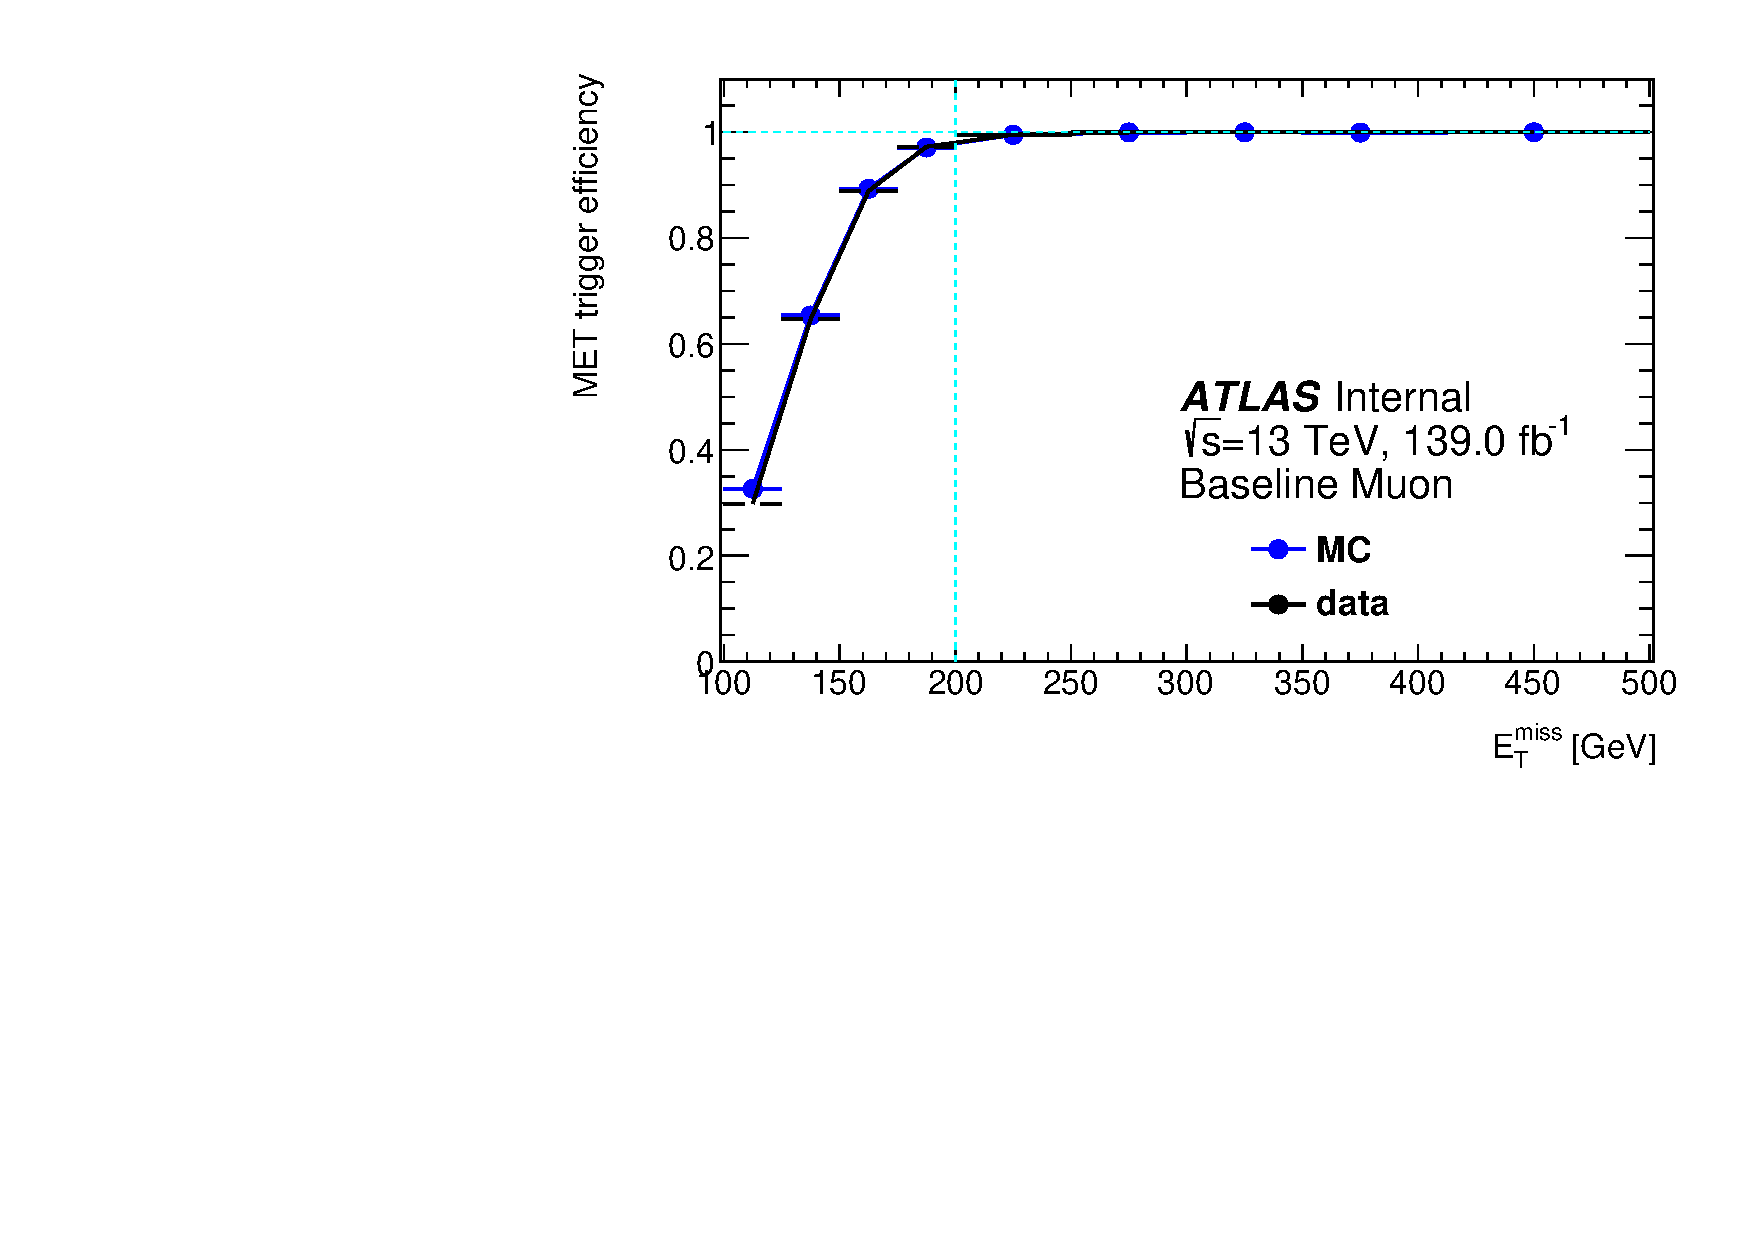
\includegraphics[width = 0.6\textwidth]{Figures/5/efficiency_baseline_muInvis.pdf}
     \caption[\met trigger efficiency in the muon channel, with muons treated as invisible in the calculation of \met.]{\met trigger efficiency, as a function of the \met lower bound with the baseline event selection applied in the muon channel, with muons treated as invisible in the calculation of \met.}
     \label{fig:metmuinvis}
  \end{figure}
 
It was found that high-\met events in the muon channel that fail the \met trigger do, however, pass the muon trigger with high efficiency. For this reason, the efficiency of a logical OR of the \met and single muon triggers is studied in the muon channel. The (\met OR single muon) trigger efficiency is calculated as follows for MC simulated events in a given region ``X":

\begin{equation}
\label{eq:met_or_single_muon_trig}
\begin{footnotesize}
\text{eff}_\text{\met OR single muon, MC, region X} = \frac{\sum_i w_i\text{ passing ($\met$ OR single muon triggers)\text{ AND }(in region X)}}{\sum_i w_i\text{ in region X}}
\end{footnotesize}
\end{equation}

\noindent where the event weight \(w_i\) in the numerator includes the scale factors to correct for the known \(<100\%\) trigger efficiency of the single muon trigger. Note that since Eq. \ref{eq:met_or_single_muon_trig} is evaluated only for MC simulated events, there is no need for an independent trigger in the numerator and denominator such as the single lepton trigger included in Eq. \ref{eq:met_trig_eff}. As shown in Figure \ref{fig:trigger_OR}, the \met OR single muon trigger is found to be effectively 100\% efficient, given the application of appropriate scale factors for the single muon trigger, in the muon channel with the baseline event selection for all lower bounds on the \met down to  \(\sim 100~\GeV\).

  \begin{figure}[htbp]
  \centering
     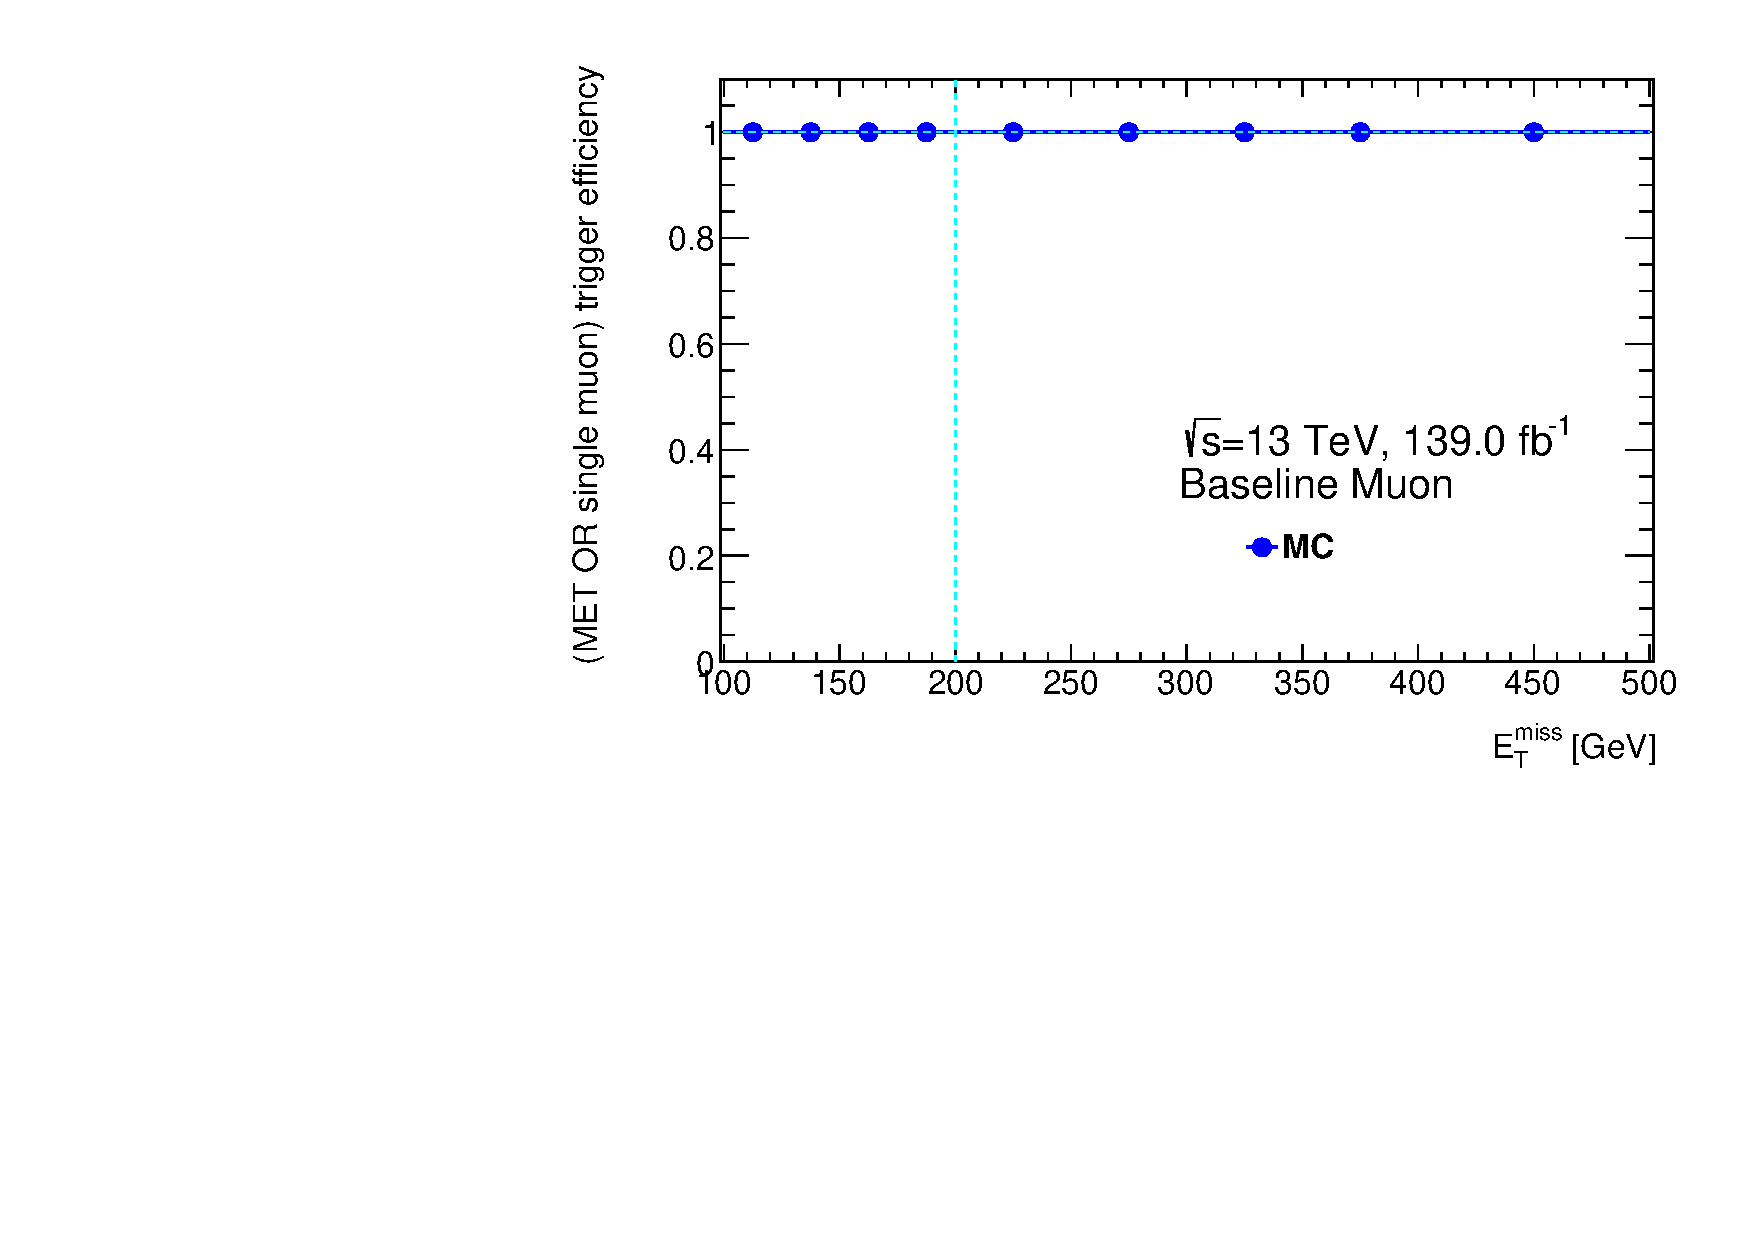
\includegraphics[width = 0.49\textwidth]{Figures/5/efficiency_baseline_muon_leptrig.pdf}
     \caption[Efficiency of the \met OR single muon trigger in the muon channel.]{Efficiency of the \met OR single muon trigger, as a function of the \met lower bound, for the baseline event selection in the muon channel.}
     \label{fig:trigger_OR}
  \end{figure}

Based on the analysis presented in this section, it is concluded that, if all events considered in the analysis are explicitly required to have passed the (\met OR single muon) trigger, the trigger efficiency is known to be 100\% for all events, except for the small subset of events with a high-\pt muon that pass the muon trigger but fail the \met trigger. For these events, scaling factors are included in the event weight to correct for the known \(<100\%\) efficiency of the single muon trigger. An additional ``trigger-matching" requirement is applied for events that fail the \met trigger but pass the single muon trigger. This requirement ensures that the final state muon object that activated the single muon trigger can be identified as the same muon object (i.e. as having originated from the same muon) that was used to reconstruct the signal muon used in the search. 
